\documentclass[12pt,a4paper,oneside,liststotoc]{report}
																															% This specifies what sort of document you intend to write.  																												 				% After that, you can include commands that influence the 																																	%	style of the whole document, or you can load packages that 																																%	add new features to the LaTeX system. To load such a package 																															 % you use the command
\usepackage[german,english]{babel}														% it provides the internationalization of LaTeX. It has to be 																															% loaded in any document, and you have to give as an option the 																													% main language you are going to use in the document
\usepackage{amsmath}																					% it contains the advanced math extensions for LaTeX. The 																																	% complete documentation should be in your LaTeX distribution; 																															 % the file is called amsdoc, and can be either dvi or pdf 																							
\usepackage{array}																						% it extends the possibility of LaTeX to handle tables, fixing 																															 % some bugs and adding new features. Using it, you can create  																												 			% very complicated and customized tables
\usepackage{color}																						% it adds support for colored text
\usepackage{geometry}																					% for easy management of document margins and the document  																												 				% size page
\geometry{a4paper,left=28mm,right=28mm,top=29mm,bottom=29mm}
\usepackage{graphicx}																					% to manage external pictures
\usepackage{psfrag}
\usepackage{eucal}																						% other mathematical symbols
\usepackage{latexsym}																					% other mathematical symbols
\usepackage{mathrsfs}																					% other mathematical symbols
\usepackage{rotating}																					% It lets you rotate any kind of object. Especially in 																																			% .tex files, generated by gnuplo, t might contain the command 
																															% "rotatebox" which is why rotating has to be activated!
\usepackage{subfigure}
\usepackage{subfig}
\usepackage{paralist}
\usepackage[nottoc]{tocbibind}
\usepackage{varwidth}
\usepackage{epstopdf}
\usepackage[numbers,square, super]{natbib}														% natbib is used to enable scientific shape of the   
																															% bibliography, numbers are activated to show the number of 
																															% each bib entry
\usepackage[latin1]{inputenc}
\usepackage{here}																							% enables the positioning of figures at "here"
\usepackage{rotating}
\usepackage{inputenc}
\usepackage{paralist}
\usepackage{pifont}																						
\usepackage{setspace}
\renewcommand{\baselinestretch}{1.3}													% set line spacing to individual value. it can be a useful 
																															% tuning value to push the pagecount of your these :)
\usepackage{import}
\usepackage{caption}
\captionsetup[figure]{skip=5pt}
\newenvironment{customitemize}{\begin{itemize}\itemsep -2pt}{\enditemize}
%
%%%%%%%%%%%%%%%%%%%%%%%%%%%%%%%%%%%%%%%%%%%%%%%%%%%%%%%%%%%%%%%%%%%%%%%%%%%%%%%%%%%%%%%%%%%%%%%%%%%%%%%%%%%%%%%%%%%%%%%%%%%%%SET AND CUSTOMIZE A PROPER NOMENCLATURE: %%%%%%%%%%%%%%%%%%%%%%%%%%%%%%%%%%%%%%%%%%%%%%%%%%%%%%%%%%%%%%%%%%%%%%%%%%%%%%%%%%%	%%%%%%%%%%%%%%%%%%%%%%%%%%%%%%%%%%%%%%%%%%%%%%%%%%%%%%%%%%%%%%%%%%%%%%%%%%%%%%%%%%%%%%%%%%%%%%%%%%%%%%%%%%%%%%%%%%%%%%%%%%%%
\usepackage{glossaries}
\usepackage{nomencl}
\makeglossary
\makenomenclature
\RequirePackage{ifthen}
%The NOMENCLATURE is subdevided in 2 parts: First we have the	"Notation" containing mathematical abbreviations and signs. Secondly we have Acronyms. Both are organized in NOMENCLATURE.
\renewcommand{\nomgroup}[1]{
\ifthenelse{\equal{#1}{A}}
{\item[\textbf{Notation}]}
{ \ifthenelse{\equal{#1}{G}}
{\item[\textbf{Acronyms}]}{}}
}
\setlength{\nomlabelwidth=40mm}																	% set LABELWIDTH between Labels and their Descriptions
\setlength{\nomitemsep=0mm}																			% set itemseparation in NOMENCLATURE
\makeatother

%%%%%%%%%%%%%%%%%%%%%%%%%%%%%%%%%%%%%%%%%%%%%%%%%%%%%%%%%%%%%%%%%%%%%%%%%%%%%%%%%%%%%%%%%%%%%%%%%%%%%%%%%%%%%%%%%%%%%%%%%%%%%
% GLOSSARY ENTRIES GO HERE %%%%%%%%%%%%%%%%%%%%%%%%%%%%%%%%%%%%%%%%%%%%%%%%%%%%%%%%%%%%%%%%%%%%%%%%%%%%%%%%%%%%%%%%%%%%%%%%% %%%%%%%%%%%%%%%%%%%%%%%%%%%%%%%%%%%%%%%%%%%%%%%%%%%%%%%%%%%%%%%%%%%%%%%%%%%%%%%%%%%%%%%%%%%%%%%%%%%%%%%%%%%%%%%%%%%%%%%%%%%%%
% Glossary entries have to be defined 2 times. The first definition "\newglossaryentry{shortform}{type=\acronymtype,name={shortform},first={longform (shortform)}}" enables the use of "\gls{shortform}". Each time you will use an acronym within your thesis, type "\gls{<acronym>}". At the first use of an acronym the acronym itself plus its signification will appear in the outline. Every further time you will employ the \gls command for this acronym, the acronym will appear in short form.
% The second is the \nomenclature definition that has to be set in order to make appear your acronyms in the nomenclature. 
% For further explanation see below:
\newglossaryentry{A/C}{type=\acronymtype,name={A/C},first={Aircraft (A/C)}}
\nomenclature[g]{A/C}{Aircraft}
%
\newglossaryentry{ILS}{type=\acronymtype,name={ILS},first={Instrument Landing System (ILS)}}
\nomenclature[g]{ILS}{Instrument Landing System}
%
\newglossaryentry{FIP}{type=\acronymtype,name={FIP},first={Flare Initial Point (FIP)}}
\nomenclature[g]{FIP}{Flare Initial Point}
%
\newglossaryentry{SC}{type=\acronymtype,name={A/C},first={Soft Computing (SC)}}
\nomenclature[g]{SC}{Soft Computing}
%
\newglossaryentry{HIS}{type=\acronymtype,name={HIS},first={Hybrid Intelligent System (HIS)}}
\nomenclature[g]{HIS}{Hybrid Intelligent System}
%
\newglossaryentry{ANFIS}{type=\acronymtype,name={ANFIS},first={Adaptive Neuro Fuzzy Inference System (ANFIS)}}
\nomenclature[g]{ANFIS}{Adaptive Neuro Inference System}
%
\newglossaryentry{ANN}{type=\acronymtype,name={ANN},first={Artificial Neural Network (ANN)}}
\nomenclature[g]{ANN}{Artificial Neural Network}
%
\newglossaryentry{AP}{type=\acronymtype,name={AP},first={Autopilot (AP)}}
\nomenclature[g]{AP}{Autopilot}
%
\newglossaryentry{LSE}{type=\acronymtype,name={LSE},first={Least Squares Estimation (LSE)}}
\nomenclature[g]{LSE}{Least Squares Estimation}
%
\newglossaryentry{OSMA}{type=\acronymtype,name={OSMA},first={Outil De Simulation Mouvement Avion (OSMA)}}
\nomenclature[g]{OSMA}{Outil De Simulation Mouvement Avion }
%
\newglossaryentry{GDE}{type=\acronymtype,name={LSE},first={Gradient Descent Method (GDE)}}
\nomenclature[g]{GDE}{Gradient Descent Method}
%
\newglossaryentry{RA}{type=\acronymtype,name={RA},first={Radio Altimeter (RA)}}
\nomenclature[g]{RA}{Radio Altimeter}
%
%%%%%%%%%%%%%%%%%%%%%%%%%%%%%%%%%%%%%%%%%%%%%%%%%%%%%%%%%%%%%%%%%%%%%%%%%%%%%%%%%%%%%%%%%%%%%%%%%%%%%%%%%%%%%%%%%%%%%%%%%%%%%
% NOTATIONS GO HERE: %%%%%%%%%%%%%%%%%%%%%%%%%%%%%%%%%%%%%%%%%%%%%%%%%%%%%%%%%%%%%%%%%%%%%%%%%%%%%%%%%%%%%%%%%%%%%%%%%%%%%%% %%%%%%%%%%%%%%%%%%%%%%%%%%%%%%%%%%%%%%%%%%%%%%%%%%%%%%%%%%%%%%%%%%%%%%%%%%%%%%%%%%%%%%%%%%%%%%%%%%%%%%%%%%%%%%%%%%%%%%%%%%%%%
\nomenclature[a]{$v_{z,IMP}$}{vertical velocity of an aircraft at touchdown [$\frac{ft}{sec}$]}
%
\nomenclature[a]{$v_{z,IMP,0}$}{estimated vertical touchdown velocity based on deterministic parameters [$\frac{ft}{sec}$]}
%
\nomenclature[a]{$v_{z,IMP,0,analytical}$}{$v_{z,IMP,0}$ estimated using an analytical formula [$\frac{ft}{sec}$]}
%
\nomenclature[a]{$v_{z,IMP,0,FIS}$}{$v_{z,IMP,0}$ estimated using a FIS [$\frac{ft}{sec}$]}
%
\nomenclature[a]{$\gamma_{FIP}$}{flight path angle at FIP [�]}
%
\nomenclature[a]{$\gamma_{rwy}$}{inclination of the runway [\%]}
%
\nomenclature[a]{m}{aircraft mass [kg]}
%
\nomenclature[a]{T}{thrust [N]}
%
\nomenclature[a]{$c_{g}$}{center of gravity in the longitudinal axis (x) [$\%$]}
%
\nomenclature[a]{$c_{L}$}{lift coefficient [-]}
%
\nomenclature[a]{$c_{D}$}{drag coefficient [-]}
%
\nomenclature[a]{$\Delta v_{z,crit}$}{buffer in the vertical touchdown velocity between an expectation superior to -10
[$\frac{ft}{sec}$] and -10 [$\frac{ft}{sec}$]}
\nomenclature[a]{$\sigma_{est}$}{estimated turbulence intesity [-]}
%
\nomenclature[a]{$v_{w}$}{vertical wind velocity [$\frac{m}{sec}$]}
%
\nomenclature[a]{$n_{z,tu}$}{turbulence load factor [-]}
%
\nomenclature[a]{$n_{z,fi}$}{fictitious load factor [-]}
%
\nomenclature[a]{$n_{z,tr}$}{true load factor [-]}
%
\nomenclature[a]{$n_{z,c}$}{commanded load factor [-]}
%
\nomenclature[a]{L}{lift [N]}
%
\nomenclature[a]{$t_{flare}$}{flare duration [sec]}
%%%%%%%%%%%%%%%%%%%%%%%%%%%%%%%%%%%%%%%%%%%%%%%%%%%%%%%%%%%%%%%%%%%%%%%%%%%%%%%%%%%%%%%%%%%%%%%%%%%%%%%%%%%%%%%%%%%%%%%%%%%%%%%%%%%%%%%%%%%%%%%%%%%%%%%%%%%%%%%%%%%%%%%%%%%%%%%%%%%%%%%%%%%%%%%%%%%%%%%%%%%%%%%%%%%%%%%%%%%%%%%%%%%%%%%%%%%%%%%%%%%%%%%%%%%%%%%%%%%%%%%%%%%%%%%%%%%%%%%%%%%%%%%%%%%%%%%%%%%%%%%%%%%%%%%%%%%%%%%%%%%%%%%%%%%%%%%%%%%%%%%%%%%%%%%%%%%%%%%%%%%%%%%%%%%%%%%%%
\begin{document}
%
\begin{titlepage}
\noindent
\parbox{0.47\textwidth}{\begin{flushleft} \input{iff_logo.pdf_tex}\\
Technical University of Braunschweig\\
Institute for Flight Guidance \end{flushleft}}
\hfill
\parbox{0.48\textwidth}{\input{airbuslogo.pdf_tex}\\
Airbus Operations SaS\\
EYCDR - Research Methods and Tools}

\vspace{2.5 cm}

%Title
{\centering \textsc First End Term Project}
\vspace{0.3 cm}
\hrule
\vspace{0.2cm}
{\huge \bfseries \noindent Vertical Touchdown Velocity \\Predictor for Passenger Aircraft in Semi Automatic Landing}
\vspace{0.2 cm}
\hrule
\vspace{1.5 cm}
{\itshape \noindent Author: cand. mach. Martin Stolle \\Matr. Nr: 2912350}\\
\vspace{8 cm}\\
%
\noindent
\flushleft{\rule{1.0\textwidth}{0.1cm}}
April 2012
\end{titlepage}
%
\section*{Acknowledgement}
The making of this thesis has not by any means been a solo effort. From my parents, both of my supervisors to my friends and my colleagues, it wouldn't have been possible to do this work without your help.\\
\\
\indent To my parents and my family, I would never have been able to make it through any step of my life without your wise, spiritual, and financial support. Thank you for having continued to support me in every way during this time at Airbus in Toulouse.\\
\\
\indent To Guilhem Puyou, my supervisor at Airbus Industries, thank you for trusting me and having the faith that I would accurately and completely accomplish this research. With your professional advice, based on your experience and your intuition, you inspired me numerous times. I appreciated the freedom you gave me during this project.\\
\\
\indent To Meiko Steen, my supervisor at the Technical University of Braunschweig, I really appreciate your support when I first made my plans to come to Airbus. I thank you for the countless advice you gave me through our phone conversations. It means a lot to me having such a cooperative and unconventional tutor.\\
\\
\indent To Matthieu Barba and Matthias Eberle, my colleagues, I thank you for having been selfless and for all of the time each of you offered me. Without your help, the implementation of my work would not have been possible.\\
\\
\indent To my friend Jan Bolting, thank you for the hours you spent patiently helping me think through my theories and providing valuable advice from an external point of view. I also thank you 
for the motivation you injected into our "Toulouse Project".\\
\\
\indent To my friend and housemate Danielle Davies, I really appreciated having you around me during the last six months. Thank you for the countless philosophizing sessions, and also for having helped progress my English skills. It really means a lot to me.\\
\\
\indent Above all, I thank God. It is He who brought me to this project and it is He who will continue to guide me throughout my life. I am looking forward to what You have lined up for me next.
%
\tableofcontents
%
\newpage
%
\listoffigures
%
\newpage
%
\printnomenclature{}
%
\chapter{Introduction}
This chapter addresses the motivation for research in pilot assistance systems. While this thesis is related to a problem in aviation, the assistance that sophisticated algorithms provide to humans can be found in numerous other fields. It has the benefit of presenting a situation in an organized fashion so that the operating human can concentrate on his outstanding skill of decision-making.   
%    
\section{Motivation}
Since the early days of passenger aircraft, there have been countless approaches and investigations to facilitate the pilot's task in passenger aviation. Civil aviation has thus become an important part of modern civilization through offering the possibility of fast, reliable and safe travel. Given the fact that air traffic volume has doubled in the past 20 years and is supposed to rise significantly in the next 20 years, maintaining the public's confidence demands a reduction in the relative number of accidents during flight operations. Examining statistics of \gls{A/C} accidents, one recognizes that even today a huge percentage occurs during the final flight phases i.e. approach and landing.\\
%
\indent To facilitate further considerations, one can separate accidents in aviation into two categories: those that are attributed to flight operations and human factors, and those which are caused by diverse technical malfunctions.\\
Recognizing that the air traffic volume augments, whereas the number of airports stagnates, the air traffic density and therefore the risk of incidents due to flight operational reasons rises dramatically at frequented airports. On the contrary, highly frequented airports are usually equipped with costly and sophisticated \gls{ILS}, enabling fully automatic landings, which citing literature and statistics, can be regarded as safer than manual landings. Nowadays the \gls{ILS} is the only commonly available and certified device, conforming the integrety and precision requirements for \gls{AP} reference signals in automatic landings. That is why automatic landings are not practiced without \gls{ILS}.\\
\indent Among the multiple approaches to cope with this bottleneck effect, the Airbus Research and Technology Department has proposed an alternative landing technique, enabling passenger aircraft to land on less frequented aerodromes, without \gls{ILS} devices at their disposal, in order to redistribute the air traffic while reducing the pilot's workload, traning costs and augmenting safety. With this technique, called semi automatic landing, the aircraft is guided manually until the \gls{FIP}, where the \gls{AP} is engaged and flares the aircraft to touchdown. When an \gls{A/C} leaves the glidepath to flare, the height of the \gls{RA} is used as vertical reference signal, which is why the \gls{ILS} is not necessary for an automatic flare and hence for a semi automatic landing. As consequence of the automatically flown flare, the risk of an aircraft incident due to the flight crew is reduced.
%
	\begin{figure}[H]
		\flushleft
		\setlength\fboxsep{3pt}
		\fbox{\input{semi_automatic_landing.pdf_tex}}
		\caption{Principle of the semi automatic landing}
	\end{figure}
%
It should be underlined that the automatic flare is conducted under use of the standard automatic flare law.\\
This concept is based on the statistical fact that in the long term, \gls{AP}s i.e. machines, cause less failed landings than human pilots. As a result, it is possible to reduce the number of failed landings due to pilot behavior without the need of an \gls{ILS} device which would be necessary to conduct a fully automatic landing.\\
\indent In that context, failed landings have to be subdivided in different cases. The highly improbable failed landing is the hazard or fatal landing, whereas the more common one is the hard landing, occurring when the \gls{A/C}'s vertical velocity at touchdown is less than -10 $[\frac{ft}{sec}]$.\\
\indent Because during fully automatic landings \gls{A/C} are accurately driven on glide beams by \gls{AP}s before the flare is initiated, the diversions of the \gls{A/C}'s attitude at FIP are within tiny margins. Consequently, during flare, the \gls{AP} has to cope with common conditions. On the contrary, in a semi automatic landing, the aircraft is flown manually down to the FIP. The \gls{A/C}'s attitude at FIP thus varies within broader margins, resulting in more challenging conditions for the autopilot. In certain cases, bad \gls{A/C} conditions at FIP accompanied by demanding environmental parameters, such as turbulence or positive runway slopes, can evoke hard landings.\\
In order to further reduce the risk of this incident, it is of interest to know the touchdown velocity of an \gls{A/C} in advance. By means of this information, it would be possible to advise the pilot so that a hard landing could be avoided.\\
\indent The aim of this thesis is to propose an onboard estimation algorithm, capable of predicting a hard landing in the moment the \gls{A/C} crosses the FIP.
%
\chapter{Theoretical Foundations}
This chapter discusses the theoretical background information, used to design the touchdown velocity prediction algorithm. In the first sections, flight mechanics during an automatic flare and parameters with impact on the touchdown velocity are outlined. The second part refers to different methods of mathematical model building.
%
\section{The Automatic Flare Maneuver}
The flare maneuver aims to smoothly reduce the vertical velocity of \gls{A/C} before touchdown. It thus builds the transition from the straight approach path to the horizontal ground roll.\\
\indent Automatic flare controllers are designed to reach touchdown rates around -2.5 $[\frac{ft}{sec}]$. The allowable vertical touchdown velocity of an airplane onto the runway is determined through several factors:\\
The passenger and crew comfort tolerates a maximum touchdown rate of -6 $[\frac{ft}{sec}]$ whereas the landing gear of most civil transport airplanes withstands a maximum touchdown rate of -10 $[\frac{ft}{sec}]$. When the touchdown rate exceeds the landing gear limitation, a hard landing occurs and the airplane has to be overhauled. Fig. 2.1 shows the flight path followed by the airplane during flare.
%
	\begin{figure}[H]
			\setlength\fboxsep{2pt}
			\fbox{\input{geom_flare_path.pdf_tex}}
			\caption{Geometry of the Flare Path during Automatic Flare}
	\end{figure}
%
Concerning the flare, it is assumed that the intended point of touchdown is 291m from the runway threshold ($x_{1}=291m$). The flare length $x_{2}$ is assumed to be 400 m. With a constant ground velocity during the flare ($V_{gnd}$), the duration of the flare ($t_{flare}$) is given by:\\
%
	\begin{equation}
		t_{flare}=\frac{\frac{h_flare}{tan\gamma_{FIP}}-291 m+400m}{V_{gnd}}
	\end{equation}
%
\indent In order to flare, the aircraft follows a curved flight path, the flare trajectory. In an automatic flare, this trajectory is predetermined right before the airplane crosses the Flare Initial Point. Airbus \gls{A/C} are controlled through load-factor commands $n_{zc}$. $n_{z}$ is the aerodynamic load factor:
%
	\begin{equation}
		g\cdot n_z=\frac{L_{0}+\delta L}{m}=1+\frac{\delta L}{m}
	\end{equation}
%
Where $L_{0}$ is the lift necessary for horizontal flight and $\delta L$ are small changes in the lift resulting in tiny flight path angles around horizontal flight.
Referring to \cite{Brockhaus2001} this value can be considered as equal in the different coordinate systems, when dealing with small flight path angles.\\
The commanded trajectory depicts a function $n_{zc}(t)$ - which is a $4^{th}$ order polynomial containing four parameters of freedom which depend on the approach velocity:
%
	\begin{equation}
		g\cdot n_{zc}(t)=a^4t+b^3t+c^2t+d
	\end{equation}
%
	\begin{equation}
		a,b,c,d=a,b,c,d(V_{gnd})
	\end{equation}
%
Fig. 2.2 depicts the automatic flare system in a Block Diagram.
%
	\begin{figure}[H]
		\setlength\fboxsep{2pt}
		\fbox{\input{bsb_automatic_flare.pdf_tex}}
		\caption{Block Diagram of the Automatic Flare Controller}
	\end{figure}
%
Assuming aircraft and \gls{AP} to be a system of first order with a time constant of $\tau$, following transfer function is given in the frequency domain:
%
	\begin{equation} 
		\frac{n_{z}}{n_{zc}}=\frac{1}{1+\tau s}\Leftrightarrow n_{z}s+\frac{n_{z}}{\tau}=\frac{n_{zc}}{\tau}
	\end{equation}
%
Transferred to the time domain it corresponds to a first order linear differential equation:
%
	\begin{equation} 
		\dot{n_{z}}+\frac{n_{z}}{\tau}=\frac{n_{zc}}{\tau}
	\end{equation}
%
Where the homogeneous equation is:
%
	\begin{equation} 
		\dot{n_{z}}+\frac{n_{z}}{\tau}=0
	\end{equation}
%
It's solution is given with:
%
	\begin{equation} 
		n_{z}(t)=K\cdot e^{\frac{-t}{\tau}}
	\end{equation}
%
The derivation of the homogeneous solution equation 2.7:
%
	\begin{equation} 
		\dot{n}_{z}=\dot{K}e^{\frac{t}{\tau}}-\frac{1}{\tau}Ke^{\frac{-t}{\tau}}
	\end{equation}
%
is inserted in equation 2.6, so that:
%
\begin{equation}
\dot{K}=\frac{n_{zc}}{\tau}e^{\frac{t}{\tau}}
\end{equation}
%
is obtained.
K is subsequently obtained using the \textit{Integration By Parts}. Including it into equation 2.5, the effective load of the airplane is:
%
	\begin{equation}
		\begin{aligned}[H]
	  g\cdot n_{z}(t)=	 \,&a\,( t^4 - 4 \tau t^3 + 12 \tau^2 t^2 - 24 \tau ^3 t + 24\tau ^4 - 24\tau ^4 e^\frac{-t}{\tau})\\
											+\,&b\,( t^3 - 3 \tau t^2 + 6  \tau^2 t   - 6  \tau ^3   + 6 \tau^3 e^\frac{-t}{\tau} )\\
											+\,&c\,( t^2 - 2 \tau t   + 2  \tau^2  e^\frac{-t}{\tau})\\
											+\,&d\,( 1   - e^ \frac{-t}{\tau})
		\end{aligned}															
	\end{equation}
%
\newpage
%
\section{Influencing Parameters}
Within this section, parameters with a significant impact on the vertical touchdown velocity are discussed through an analysis of flight mechanics during the flare maneuver.  
%
\subsection{Initial flight path angle and ground velocity}
As shown before, the commanded flare trajectory is a $4^{th}$ order polynomial $n_{zc}(t)$. The profile of the effective vertical velocity $v_{z}(t)$ during the flare is received by integration of the effective load factor $n_{z}(t)$:\\
%
	\begin{equation} 
		\begin{aligned}[H]
				v_{z}(t)=\, &a\,( \frac{1}{5}t^5 - \tau t^4 + 4\tau ^2 t^3 - 12\tau ^3 t^2 + 24\tau ^5 - 24\tau^5 e^\frac{-t}{\tau})\\
								+\, &b\,( \frac{1}{4}t^4 - \tau t^3 + 3\tau ^2 t^2 - 6 \tau ^3t    + 6 \tau^4  + 6 \tau^4  e^\frac{-t}{\tau} )\\
								+\, &c\,( \frac{1}{3}t^3 - \tau t^2 + 2\tau ^2t    - 2 \tau^3      +	 \tau^3 e^\frac{-t}{\tau})\\
								+\, &d\,(            t   - \tau     +  \tau e^ \frac{-t}{\tau})\\
								+\, &v_{z,FIP}\\
			\end{aligned}
	\end{equation}
%
The constant of integration $v_{z,FIP}$ is the sink rate of the \gls{A/C} at Flare Initial Point. It is defined as:
%
	\begin{equation} 
		v_{z \, FIP}=V_{gnd}\cdot tan(\gamma_{FIP})
	\end{equation}
%
As a consequence, the vertical touchdown velocity is impacted by the initial flight path angle $\gamma_{FIP}$ and the ground velocity $V_{gnd}$:
%
	\begin{equation}
		v_{z,IMP}=v_{z,IMP}(\gamma_{FIP},V_{gnd})	
	\end{equation}
%
Figs. 2.3 and 2.4 illustrate the individual influence of the two parameters on the vertical touchdown velocity while freezing the other value to default. for an Airbus \gls{A/C}. These results have been obtained through simulation.
%	
	\begin{figure}[H]
		% GNUPLOT: LaTeX picture with Postscript
\begingroup
  \makeatletter
  \providecommand\color[2][]{%
    \GenericError{(gnuplot) \space\space\space\@spaces}{%
      Package color not loaded in conjunction with
      terminal option `colourtext'%
    }{See the gnuplot documentation for explanation.%
    }{Either use 'blacktext' in gnuplot or load the package
      color.sty in LaTeX.}%
    \renewcommand\color[2][]{}%
  }%
  \providecommand\includegraphics[2][]{%
    \GenericError{(gnuplot) \space\space\space\@spaces}{%
      Package graphicx or graphics not loaded%
    }{See the gnuplot documentation for explanation.%
    }{The gnuplot epslatex terminal needs graphicx.sty or graphics.sty.}%
    \renewcommand\includegraphics[2][]{}%
  }%
  \providecommand\rotatebox[2]{#2}%
  \@ifundefined{ifGPcolor}{%
    \newif\ifGPcolor
    \GPcolorfalse
  }{}%
  \@ifundefined{ifGPblacktext}{%
    \newif\ifGPblacktext
    \GPblacktexttrue
  }{}%
  % define a \g@addto@macro without @ in the name:
  \let\gplgaddtomacro\g@addto@macro
  % define empty templates for all commands taking text:
  \gdef\gplbacktext{}%
  \gdef\gplfronttext{}%
  \makeatother
  \ifGPblacktext
    % no textcolor at all
    \def\colorrgb#1{}%
    \def\colorgray#1{}%
  \else
    % gray or color?
    \ifGPcolor
      \def\colorrgb#1{\color[rgb]{#1}}%
      \def\colorgray#1{\color[gray]{#1}}%
      \expandafter\def\csname LTw\endcsname{\color{white}}%
      \expandafter\def\csname LTb\endcsname{\color{black}}%
      \expandafter\def\csname LTa\endcsname{\color{black}}%
      \expandafter\def\csname LT0\endcsname{\color[rgb]{1,0,0}}%
      \expandafter\def\csname LT1\endcsname{\color[rgb]{0,1,0}}%
      \expandafter\def\csname LT2\endcsname{\color[rgb]{0,0,1}}%
      \expandafter\def\csname LT3\endcsname{\color[rgb]{1,0,1}}%
      \expandafter\def\csname LT4\endcsname{\color[rgb]{0,1,1}}%
      \expandafter\def\csname LT5\endcsname{\color[rgb]{1,1,0}}%
      \expandafter\def\csname LT6\endcsname{\color[rgb]{0,0,0}}%
      \expandafter\def\csname LT7\endcsname{\color[rgb]{1,0.3,0}}%
      \expandafter\def\csname LT8\endcsname{\color[rgb]{0.5,0.5,0.5}}%
    \else
      % gray
      \def\colorrgb#1{\color{black}}%
      \def\colorgray#1{\color[gray]{#1}}%
      \expandafter\def\csname LTw\endcsname{\color{white}}%
      \expandafter\def\csname LTb\endcsname{\color{black}}%
      \expandafter\def\csname LTa\endcsname{\color{black}}%
      \expandafter\def\csname LT0\endcsname{\color{black}}%
      \expandafter\def\csname LT1\endcsname{\color{black}}%
      \expandafter\def\csname LT2\endcsname{\color{black}}%
      \expandafter\def\csname LT3\endcsname{\color{black}}%
      \expandafter\def\csname LT4\endcsname{\color{black}}%
      \expandafter\def\csname LT5\endcsname{\color{black}}%
      \expandafter\def\csname LT6\endcsname{\color{black}}%
      \expandafter\def\csname LT7\endcsname{\color{black}}%
      \expandafter\def\csname LT8\endcsname{\color{black}}%
    \fi
  \fi
  \setlength{\unitlength}{0.0500bp}%
  \begin{picture}(9070.00,3400.00)%
    \gplgaddtomacro\gplbacktext{%
      \csname LTb\endcsname%
      \put(814,704){\makebox(0,0)[r]{\strut{}-25}}%
      \csname LTb\endcsname%
      \put(814,1243){\makebox(0,0)[r]{\strut{}-20}}%
      \csname LTb\endcsname%
      \put(814,1782){\makebox(0,0)[r]{\strut{}-15}}%
      \csname LTb\endcsname%
      \put(814,2321){\makebox(0,0)[r]{\strut{}-10}}%
      \csname LTb\endcsname%
      \put(814,2860){\makebox(0,0)[r]{\strut{}-5}}%
      \csname LTb\endcsname%
      \put(814,3399){\makebox(0,0)[r]{\strut{} 0}}%
      \csname LTb\endcsname%
      \put(946,484){\makebox(0,0){\strut{}-5.75}}%
      \csname LTb\endcsname%
      \put(1590,484){\makebox(0,0){\strut{}-5.5}}%
      \csname LTb\endcsname%
      \put(2234,484){\makebox(0,0){\strut{}-5.25}}%
      \csname LTb\endcsname%
      \put(2878,484){\makebox(0,0){\strut{}-5}}%
      \csname LTb\endcsname%
      \put(3522,484){\makebox(0,0){\strut{}-4.75}}%
      \csname LTb\endcsname%
      \put(4166,484){\makebox(0,0){\strut{}-4.5}}%
      \csname LTb\endcsname%
      \put(4809,484){\makebox(0,0){\strut{}-4.25}}%
      \csname LTb\endcsname%
      \put(5453,484){\makebox(0,0){\strut{}-4}}%
      \csname LTb\endcsname%
      \put(6097,484){\makebox(0,0){\strut{}-3.75}}%
      \csname LTb\endcsname%
      \put(6741,484){\makebox(0,0){\strut{}-3.5}}%
      \csname LTb\endcsname%
      \put(7385,484){\makebox(0,0){\strut{}-3.25}}%
      \csname LTb\endcsname%
      \put(8029,484){\makebox(0,0){\strut{}-3}}%
      \csname LTb\endcsname%
      \put(8673,484){\makebox(0,0){\strut{}-2.75}}%
      \put(176,2051){\rotatebox{-270}{\makebox(0,0){\strut{}$v_{z,IMP}\,[\frac{ft}{sec}]$}}}%
      \put(4809,154){\makebox(0,0){\strut{}$\gamma_{FIP}[^{\circ}]$}}%
    }%
    \gplgaddtomacro\gplfronttext{%
    }%
    \gplbacktext
    \put(0,0){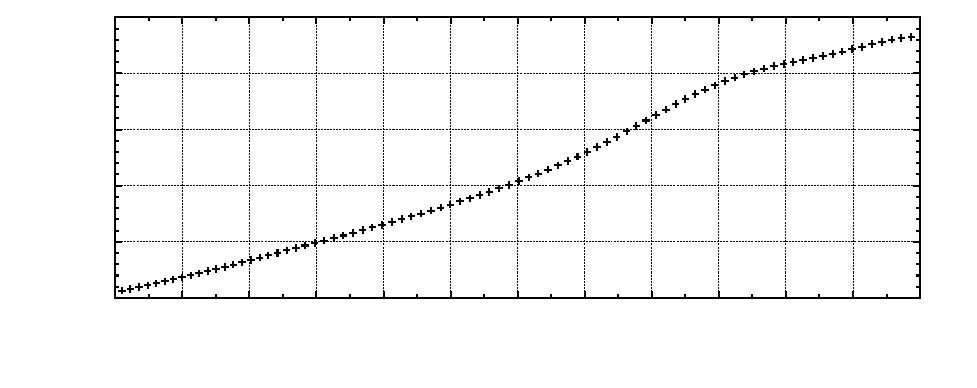
\includegraphics{GAMGL_impact}}%
    \gplfronttext
  \end{picture}%
\endgroup

		\caption{Influence of $\gamma_{FIP}$ on $v_{z,IMP}$}
	\end{figure}
%
	\begin{figure}[H]
		% GNUPLOT: LaTeX picture with Postscript
\begingroup
  \makeatletter
  \providecommand\color[2][]{%
    \GenericError{(gnuplot) \space\space\space\@spaces}{%
      Package color not loaded in conjunction with
      terminal option `colourtext'%
    }{See the gnuplot documentation for explanation.%
    }{Either use 'blacktext' in gnuplot or load the package
      color.sty in LaTeX.}%
    \renewcommand\color[2][]{}%
  }%
  \providecommand\includegraphics[2][]{%
    \GenericError{(gnuplot) \space\space\space\@spaces}{%
      Package graphicx or graphics not loaded%
    }{See the gnuplot documentation for explanation.%
    }{The gnuplot epslatex terminal needs graphicx.sty or graphics.sty.}%
    \renewcommand\includegraphics[2][]{}%
  }%
  \providecommand\rotatebox[2]{#2}%
  \@ifundefined{ifGPcolor}{%
    \newif\ifGPcolor
    \GPcolorfalse
  }{}%
  \@ifundefined{ifGPblacktext}{%
    \newif\ifGPblacktext
    \GPblacktexttrue
  }{}%
  % define a \g@addto@macro without @ in the name:
  \let\gplgaddtomacro\g@addto@macro
  % define empty templates for all commands taking text:
  \gdef\gplbacktext{}%
  \gdef\gplfronttext{}%
  \makeatother
  \ifGPblacktext
    % no textcolor at all
    \def\colorrgb#1{}%
    \def\colorgray#1{}%
  \else
    % gray or color?
    \ifGPcolor
      \def\colorrgb#1{\color[rgb]{#1}}%
      \def\colorgray#1{\color[gray]{#1}}%
      \expandafter\def\csname LTw\endcsname{\color{white}}%
      \expandafter\def\csname LTb\endcsname{\color{black}}%
      \expandafter\def\csname LTa\endcsname{\color{black}}%
      \expandafter\def\csname LT0\endcsname{\color[rgb]{1,0,0}}%
      \expandafter\def\csname LT1\endcsname{\color[rgb]{0,1,0}}%
      \expandafter\def\csname LT2\endcsname{\color[rgb]{0,0,1}}%
      \expandafter\def\csname LT3\endcsname{\color[rgb]{1,0,1}}%
      \expandafter\def\csname LT4\endcsname{\color[rgb]{0,1,1}}%
      \expandafter\def\csname LT5\endcsname{\color[rgb]{1,1,0}}%
      \expandafter\def\csname LT6\endcsname{\color[rgb]{0,0,0}}%
      \expandafter\def\csname LT7\endcsname{\color[rgb]{1,0.3,0}}%
      \expandafter\def\csname LT8\endcsname{\color[rgb]{0.5,0.5,0.5}}%
    \else
      % gray
      \def\colorrgb#1{\color{black}}%
      \def\colorgray#1{\color[gray]{#1}}%
      \expandafter\def\csname LTw\endcsname{\color{white}}%
      \expandafter\def\csname LTb\endcsname{\color{black}}%
      \expandafter\def\csname LTa\endcsname{\color{black}}%
      \expandafter\def\csname LT0\endcsname{\color{black}}%
      \expandafter\def\csname LT1\endcsname{\color{black}}%
      \expandafter\def\csname LT2\endcsname{\color{black}}%
      \expandafter\def\csname LT3\endcsname{\color{black}}%
      \expandafter\def\csname LT4\endcsname{\color{black}}%
      \expandafter\def\csname LT5\endcsname{\color{black}}%
      \expandafter\def\csname LT6\endcsname{\color{black}}%
      \expandafter\def\csname LT7\endcsname{\color{black}}%
      \expandafter\def\csname LT8\endcsname{\color{black}}%
    \fi
  \fi
  \setlength{\unitlength}{0.0500bp}%
  \begin{picture}(9070.00,3400.00)%
    \gplgaddtomacro\gplbacktext{%
      \csname LTb\endcsname%
      \put(682,1051){\makebox(0,0)[r]{\strut{}-3}}%
      \csname LTb\endcsname%
      \put(682,1746){\makebox(0,0)[r]{\strut{}-2}}%
      \csname LTb\endcsname%
      \put(682,2440){\makebox(0,0)[r]{\strut{}-1}}%
      \csname LTb\endcsname%
      \put(682,3135){\makebox(0,0)[r]{\strut{} 0}}%
      \csname LTb\endcsname%
      \put(1528,484){\makebox(0,0){\strut{} 120}}%
      \csname LTb\endcsname%
      \put(2957,484){\makebox(0,0){\strut{} 130}}%
      \csname LTb\endcsname%
      \put(4386,484){\makebox(0,0){\strut{} 140}}%
      \csname LTb\endcsname%
      \put(5815,484){\makebox(0,0){\strut{} 150}}%
      \csname LTb\endcsname%
      \put(7244,484){\makebox(0,0){\strut{} 160}}%
      \csname LTb\endcsname%
      \put(8673,484){\makebox(0,0){\strut{} 170}}%
      \put(176,1919){\rotatebox{-270}{\makebox(0,0){\strut{}$v_{z,IMP}\,[\frac{ft}{sec}]$}}}%
      \put(4743,154){\makebox(0,0){\strut{}$V_{gnd}$\,[kt]}}%
    }%
    \gplgaddtomacro\gplfronttext{%
    }%
    \gplbacktext
    \put(0,0){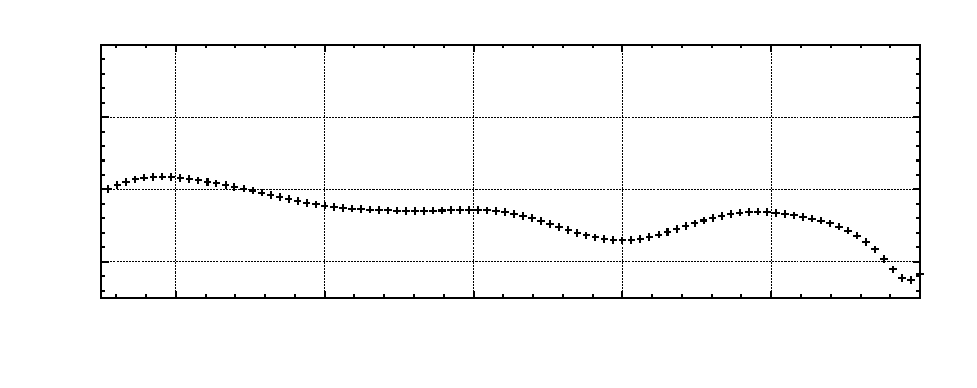
\includegraphics{V_GND_impact}}%
    \gplfronttext
  \end{picture}%
\endgroup

		\caption{Influence of $V_{gnd}$ on $v_{z,IMP}$}
	\end{figure}
%
\subsection{Runway Slope}
Equation 2.13 assumes a leveled runway. In reality, non-leveled runways occur frequently. This inclination, called runway slope, is indicated in $\%$. Depending on its sign, the inclination can raise or reduce the touchdown velocity as Fig. 2.5 illustrates. If the \gls{AP} does not consider the runway slope, the touchdown velocity is the sum of the aircraft's vertical velocity at touchdown ($v_{z}$) and the component due to the slope ($v_{z\,rwy}$).
%
	\begin{equation}
		v_{z,IMP}=v_{z}+v_{z,rwy}
	\end{equation}
%
Airbus flare controllers are able to compensate for a huge part of this effect. The \gls{RA}, which is activated during the flare, therefore differentiates the measured height in order to recognize unleveled runways. It is hence possible to adapt the flare controller to local environmental conditions. Nevertheless a small effect can remain on the vertical touchdown velocity, which is why equation 2.14 is extended:
% 
	\begin{equation}
		v_{z,IMP}=v_{z,IMP}(\gamma_{FIP},V_{gnd},\gamma_{rwy})	
	\end{equation}
% 
%
	\begin{figure}[here]
		\begin{center}
		\setlength\fboxsep{5pt}
				\subfigure[Negative Inclination]{\fbox{\input{rwy_slope_1.pdf_tex}}}
				\subfigure[Positive Inclination]{\fbox{\input{rwy_slope_2.pdf_tex}}}
				\caption{Runway Slope Influence}
		\end{center}
	\end{figure}
%
%
	\begin{figure}[H]
		% GNUPLOT: LaTeX picture with Postscript
\begingroup
  \makeatletter
  \providecommand\color[2][]{%
    \GenericError{(gnuplot) \space\space\space\@spaces}{%
      Package color not loaded in conjunction with
      terminal option `colourtext'%
    }{See the gnuplot documentation for explanation.%
    }{Either use 'blacktext' in gnuplot or load the package
      color.sty in LaTeX.}%
    \renewcommand\color[2][]{}%
  }%
  \providecommand\includegraphics[2][]{%
    \GenericError{(gnuplot) \space\space\space\@spaces}{%
      Package graphicx or graphics not loaded%
    }{See the gnuplot documentation for explanation.%
    }{The gnuplot epslatex terminal needs graphicx.sty or graphics.sty.}%
    \renewcommand\includegraphics[2][]{}%
  }%
  \providecommand\rotatebox[2]{#2}%
  \@ifundefined{ifGPcolor}{%
    \newif\ifGPcolor
    \GPcolorfalse
  }{}%
  \@ifundefined{ifGPblacktext}{%
    \newif\ifGPblacktext
    \GPblacktexttrue
  }{}%
  % define a \g@addto@macro without @ in the name:
  \let\gplgaddtomacro\g@addto@macro
  % define empty templates for all commands taking text:
  \gdef\gplbacktext{}%
  \gdef\gplfronttext{}%
  \makeatother
  \ifGPblacktext
    % no textcolor at all
    \def\colorrgb#1{}%
    \def\colorgray#1{}%
  \else
    % gray or color?
    \ifGPcolor
      \def\colorrgb#1{\color[rgb]{#1}}%
      \def\colorgray#1{\color[gray]{#1}}%
      \expandafter\def\csname LTw\endcsname{\color{white}}%
      \expandafter\def\csname LTb\endcsname{\color{black}}%
      \expandafter\def\csname LTa\endcsname{\color{black}}%
      \expandafter\def\csname LT0\endcsname{\color[rgb]{1,0,0}}%
      \expandafter\def\csname LT1\endcsname{\color[rgb]{0,1,0}}%
      \expandafter\def\csname LT2\endcsname{\color[rgb]{0,0,1}}%
      \expandafter\def\csname LT3\endcsname{\color[rgb]{1,0,1}}%
      \expandafter\def\csname LT4\endcsname{\color[rgb]{0,1,1}}%
      \expandafter\def\csname LT5\endcsname{\color[rgb]{1,1,0}}%
      \expandafter\def\csname LT6\endcsname{\color[rgb]{0,0,0}}%
      \expandafter\def\csname LT7\endcsname{\color[rgb]{1,0.3,0}}%
      \expandafter\def\csname LT8\endcsname{\color[rgb]{0.5,0.5,0.5}}%
    \else
      % gray
      \def\colorrgb#1{\color{black}}%
      \def\colorgray#1{\color[gray]{#1}}%
      \expandafter\def\csname LTw\endcsname{\color{white}}%
      \expandafter\def\csname LTb\endcsname{\color{black}}%
      \expandafter\def\csname LTa\endcsname{\color{black}}%
      \expandafter\def\csname LT0\endcsname{\color{black}}%
      \expandafter\def\csname LT1\endcsname{\color{black}}%
      \expandafter\def\csname LT2\endcsname{\color{black}}%
      \expandafter\def\csname LT3\endcsname{\color{black}}%
      \expandafter\def\csname LT4\endcsname{\color{black}}%
      \expandafter\def\csname LT5\endcsname{\color{black}}%
      \expandafter\def\csname LT6\endcsname{\color{black}}%
      \expandafter\def\csname LT7\endcsname{\color{black}}%
      \expandafter\def\csname LT8\endcsname{\color{black}}%
    \fi
  \fi
  \setlength{\unitlength}{0.0500bp}%
  \begin{picture}(9070.00,3400.00)%
    \gplgaddtomacro\gplbacktext{%
      \csname LTb\endcsname%
      \put(946,1109){\makebox(0,0)[r]{\strut{}-5}}%
      \csname LTb\endcsname%
      \put(946,2122){\makebox(0,0)[r]{\strut{}-2.5}}%
      \csname LTb\endcsname%
      \put(946,3135){\makebox(0,0)[r]{\strut{} 0}}%
      \csname LTb\endcsname%
      \put(1315,484){\makebox(0,0){\strut{}-0.75}}%
      \csname LTb\endcsname%
      \put(2502,484){\makebox(0,0){\strut{}-0.5}}%
      \csname LTb\endcsname%
      \put(3689,484){\makebox(0,0){\strut{}-0.25}}%
      \csname LTb\endcsname%
      \put(4876,484){\makebox(0,0){\strut{} 0}}%
      \csname LTb\endcsname%
      \put(6062,484){\makebox(0,0){\strut{} 0.25}}%
      \csname LTb\endcsname%
      \put(7249,484){\makebox(0,0){\strut{} 0.5}}%
      \csname LTb\endcsname%
      \put(8436,484){\makebox(0,0){\strut{} 0.75}}%
      \put(176,1919){\rotatebox{-270}{\makebox(0,0){\strut{}$v_{z,IMP}\,[\frac{ft}{sec}]$}}}%
      \put(4875,154){\makebox(0,0){\strut{}Runway Slope [$\%$]}}%
    }%
    \gplgaddtomacro\gplfronttext{%
    }%
    \gplbacktext
    \put(0,0){\includegraphics{gampist_impact}}%
    \gplfronttext
  \end{picture}%
\endgroup


		\caption{Influence of the Runway Slope}
	\end{figure}
%
\subsection{Pilot Induced Load}
As mentioned in the introduction, the approach of a semi automatic landing is done manually without lateral and vertical reference to an \gls{ILS} device.
Taking into account the human's factor, the trajectory of the aircraft varies within broader margins since the pilot has one important reference signal less at his disposal.
Equation 2.17 describes the load factor depending on the flight path angle and its derivative.
\begin{equation}
n_{z}=\frac{V}{g}\dot{\gamma}+cos(\gamma)
\end{equation}
\\
During an automatically flown approach the \gls{A/C} is stabilized on the glide slope which is why its load factor remains 1:
%
	\begin{equation}
		n_{z}=\frac{V}{g}\dot{\gamma}+cos(\gamma)\approx 1
	\end{equation}
%
The load factor at FIP is thus also 1.\\
In a manual approach without \gls{ILS} reference, the occurrence of slightly different load factors is highly probable. That is why the load factor at FIP can vary. Assuming the application of a flare controller that is not specifically adapted to the semi automatic landing, i.e. a flare controller designed for an initial operating point ${n_{z}=1}$, the initial load factor has an influence on the vertical touchdown velocity, when the initial condition of the command variable ($n_{z}$) varies. Equation 2.16 is thus extended to:
%
	\begin{equation}
		v_{z,IMP}=v_{z,IMP}(\gamma_{FIP},V_{gnd},\gamma_{rwy},n_{z})
	\end{equation}
%
%		
\subsection{Vertical Turbulences}
Besides the parameters discussed in the previous section, it is important to consider the dynamic atmosphere's influence on an aircraft. The vertical wind impacts the touchdown velocity since it has an influence on the vertical velocity of an aircraft:\\
on the one hand, in the moment the aircraft touchdowns (ttd). Depending on the orientation of the vertical wind velocity at the moment of touchdown, one turbulence level can, comparable to the runway slope, aggravate or neutralize the situation (Fig. 2.7).\\
%
	\begin{figure}[H]                                   
		% GNUPLOT: LaTeX picture with Postscript
\begingroup
  \makeatletter
  \providecommand\color[2][]{%
    \GenericError{(gnuplot) \space\space\space\@spaces}{%
      Package color not loaded in conjunction with
      terminal option `colourtext'%
    }{See the gnuplot documentation for explanation.%
    }{Either use 'blacktext' in gnuplot or load the package
      color.sty in LaTeX.}%
    \renewcommand\color[2][]{}%
  }%
  \providecommand\includegraphics[2][]{%
    \GenericError{(gnuplot) \space\space\space\@spaces}{%
      Package graphicx or graphics not loaded%
    }{See the gnuplot documentation for explanation.%
    }{The gnuplot epslatex terminal needs graphicx.sty or graphics.sty.}%
    \renewcommand\includegraphics[2][]{}%
  }%
  \providecommand\rotatebox[2]{#2}%
  \@ifundefined{ifGPcolor}{%
    \newif\ifGPcolor
    \GPcolorfalse
  }{}%
  \@ifundefined{ifGPblacktext}{%
    \newif\ifGPblacktext
    \GPblacktexttrue
  }{}%
  % define a \g@addto@macro without @ in the name:
  \let\gplgaddtomacro\g@addto@macro
  % define empty templates for all commands taking text:
  \gdef\gplbacktext{}%
  \gdef\gplfronttext{}%
  \makeatother
  \ifGPblacktext
    % no textcolor at all
    \def\colorrgb#1{}%
    \def\colorgray#1{}%
  \else
    % gray or color?
    \ifGPcolor
      \def\colorrgb#1{\color[rgb]{#1}}%
      \def\colorgray#1{\color[gray]{#1}}%
      \expandafter\def\csname LTw\endcsname{\color{white}}%
      \expandafter\def\csname LTb\endcsname{\color{black}}%
      \expandafter\def\csname LTa\endcsname{\color{black}}%
      \expandafter\def\csname LT0\endcsname{\color[rgb]{1,0,0}}%
      \expandafter\def\csname LT1\endcsname{\color[rgb]{0,1,0}}%
      \expandafter\def\csname LT2\endcsname{\color[rgb]{0,0,1}}%
      \expandafter\def\csname LT3\endcsname{\color[rgb]{1,0,1}}%
      \expandafter\def\csname LT4\endcsname{\color[rgb]{0,1,1}}%
      \expandafter\def\csname LT5\endcsname{\color[rgb]{1,1,0}}%
      \expandafter\def\csname LT6\endcsname{\color[rgb]{0,0,0}}%
      \expandafter\def\csname LT7\endcsname{\color[rgb]{1,0.3,0}}%
      \expandafter\def\csname LT8\endcsname{\color[rgb]{0.5,0.5,0.5}}%
    \else
      % gray
      \def\colorrgb#1{\color{black}}%
      \def\colorgray#1{\color[gray]{#1}}%
      \expandafter\def\csname LTw\endcsname{\color{white}}%
      \expandafter\def\csname LTb\endcsname{\color{black}}%
      \expandafter\def\csname LTa\endcsname{\color{black}}%
      \expandafter\def\csname LT0\endcsname{\color{black}}%
      \expandafter\def\csname LT1\endcsname{\color{black}}%
      \expandafter\def\csname LT2\endcsname{\color{black}}%
      \expandafter\def\csname LT3\endcsname{\color{black}}%
      \expandafter\def\csname LT4\endcsname{\color{black}}%
      \expandafter\def\csname LT5\endcsname{\color{black}}%
      \expandafter\def\csname LT6\endcsname{\color{black}}%
      \expandafter\def\csname LT7\endcsname{\color{black}}%
      \expandafter\def\csname LT8\endcsname{\color{black}}%
    \fi
  \fi
  \setlength{\unitlength}{0.0500bp}%
  \begin{picture}(9070.00,3118.00)%
    \gplgaddtomacro\gplbacktext{%
      \csname LTb\endcsname%
      \put(946,923){\makebox(0,0)[r]{\strut{}-10}}%
      \csname LTb\endcsname%
      \put(946,1472){\makebox(0,0)[r]{\strut{}-7.5}}%
      \csname LTb\endcsname%
      \put(946,2020){\makebox(0,0)[r]{\strut{}-5}}%
      \csname LTb\endcsname%
      \put(946,2569){\makebox(0,0)[r]{\strut{}-2.5}}%
      \csname LTb\endcsname%
      \put(946,3117){\makebox(0,0)[r]{\strut{} 0}}%
      \csname LTb\endcsname%
      \put(1078,484){\makebox(0,0){\strut{} 30}}%
      \csname LTb\endcsname%
      \put(2597,484){\makebox(0,0){\strut{} 31}}%
      \csname LTb\endcsname%
      \put(4116,484){\makebox(0,0){\strut{} 32}}%
      \csname LTb\endcsname%
      \put(5635,484){\makebox(0,0){\strut{} 33}}%
      \csname LTb\endcsname%
      \put(7154,484){\makebox(0,0){\strut{} 34}}%
      \csname LTb\endcsname%
      \put(8673,484){\makebox(0,0){\strut{} 35}}%
      \put(176,1910){\rotatebox{-270}{\makebox(0,0){\strut{}$v_{z,IMP}\,[\frac{ft}{sec}]$}}}%
      \put(4875,154){\makebox(0,0){\strut{}time [sec]}}%
    }%
    \gplgaddtomacro\gplfronttext{%
    }%
    \gplbacktext
    \put(0,0){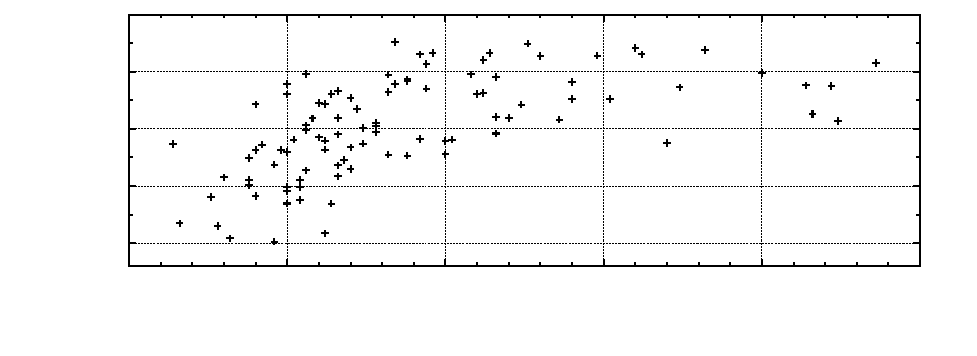
\includegraphics{turbulence_impact}}%
    \gplfronttext
  \end{picture}%
\endgroup

		\caption{Influence of Turbulences}
	\end{figure}
%
On the other hand, the vertical wind continuously impacts the landing maneuver, through disturbance of the aircraft control.
Since turbulences are a random change of the vertical wind velocity, it is complicated to describe the influence of turbulences analytically. In practice, this is due to the countless nonlinear effects, which makes describing turbulences this way unpromising and therefore uncommon.\\
In this thesis turbulences are considered as a Gaussian-distributed and random process, following a proposition by aviation authorities. According to \citet{Brockhaus2001} and \citet{Roskam1995} turbulences can be described stochastically, under use of following formula:\\
%
	\begin{equation}
		\sigma=\sqrt{\frac{1}{t_o}\int_{0}^{t_{o}} v_{w}^2(t)dt}
	\end{equation}
%
Where ($t_{0}$) is the time of observation, ($v_{w}$) the vertical wind velocity and most importantly ($\sigma$) the turbulence intensity.
%\newpage
\section{Mathematical System Modeling}
This section explains the basic functionalities of the mathematical methods that have been used to design the prediction algorithm.
%
\subsection{Fuzzy Logic}
Fuzzy Logic enables the possibility to deal with vague, imprecise and uncertain data or knowledge under use of the theory of fuzzy sets. Contrary to most methods of handling imprecision, Fuzzy Logic is concerned with the use of fuzzy values that capture the meanings of words, human thinking and decision making.\\
Fuzzy sets were invented in 1965 by Lafti Zadeh to extend classical crisp sets. In contrast to a crisp set i.e. a set of boolean values, the fuzzy set is multi-valued. In the classical boolean theory, an element x can only belong to set A or not. This is what defines the set as crisp. In consequence of the sharp boundary, each member of the set obtains the value of 1 and each element outside the boundary gets the value 0.
%
	\begin{equation}  		
		\mu_A(x)=1 \text  {    if x is totally in A;  }
	\end{equation}
%
	\begin{equation}
		\mu_A(x)=0 \text  {    if x is not in A;      }								 
	\end{equation}
%
Contrary to a boolean set, fuzzy sets exhibit fuzzy boundaries.
%
	\begin{equation}
		\mu_A(x):A\rightarrow[0,1]
	\end{equation}	
%
where:
%
	\begin{equation}
		0<	\mu_A(x)<1\text   {    if x is partly in A.   }
	\end{equation}
%
with $\mu_A(x)$ as the membership function.
\indent The term "Logic" stands for the art of expressing knowledge by transforming crisp inputs in membership degrees and treating them with application of simple rules.
%
\subsubsection{Fuzzy Inference Systems:}
FIS are expert systems based on the theory of fuzzy sets and Fuzzy Logic. An expert system basically tries to emulate the reasoning of a human expert. In FIS, this is done by storing the human knowledge expressed by simple rules.\\
The output in a FIS is computed in different steps:
%
	\begin{compactitem}[$\bullet$]
	  \setlength{\topsep}{0.8cm}
	  \setlength{\parsep}{0.8cm}
		\item Fuzzification
		\item Rule Evaluation
		\item Deduction of Output
	\end{compactitem}
%
\textbf{Fuzzification:}
Within the fuzzification, the crisp input-values of the (k) inputs ($x_{1},...,x_{k})$ are transformed into grades of membership, ranging from 0 to 1. For a domain X, a fuzzy set A over X is defined by a membership function $\mu_A(x)\Rightarrow[0,1]$ as mentioned above. The idea of this step is to allocate linguistic variables to each input value. For each input ($x_{1},...,x_{k}$) linguistic variables are proposed by an expert. The shape of the membership function is also defined by the expert. An expert is a person who is able to rate the importance of an input due to his knowledge. This way, each input value can address at least one attribute, depending on the crisp input value. Fig. 2.8 illustrates the procedure of fuzzification for a system with two inputs ($x_{1}$, $x_{2}$), four attributes ($A1,A2,A3,A4$) expressed through trapezoidal membership functions.
%
	\begin{figure}[H]                                   
		\begin{center}
			\setlength\fboxsep{2pt}
			\fbox{\begin{minipage}[t]{0.96\textwidth}
					\begingroup
						% GNUPLOT: LaTeX picture with Postscript
\begingroup
  \makeatletter
  \providecommand\color[2][]{%
    \GenericError{(gnuplot) \space\space\space\@spaces}{%
      Package color not loaded in conjunction with
      terminal option `colourtext'%
    }{See the gnuplot documentation for explanation.%
    }{Either use 'blacktext' in gnuplot or load the package
      color.sty in LaTeX.}%
    \renewcommand\color[2][]{}%
  }%
  \providecommand\includegraphics[2][]{%
    \GenericError{(gnuplot) \space\space\space\@spaces}{%
      Package graphicx or graphics not loaded%
    }{See the gnuplot documentation for explanation.%
    }{The gnuplot epslatex terminal needs graphicx.sty or graphics.sty.}%
    \renewcommand\includegraphics[2][]{}%
  }%
  \providecommand\rotatebox[2]{#2}%
  \@ifundefined{ifGPcolor}{%
    \newif\ifGPcolor
    \GPcolorfalse
  }{}%
  \@ifundefined{ifGPblacktext}{%
    \newif\ifGPblacktext
    \GPblacktexttrue
  }{}%
  % define a \g@addto@macro without @ in the name:
  \let\gplgaddtomacro\g@addto@macro
  % define empty templates for all commands taking text:
  \gdef\gplbacktext{}%
  \gdef\gplfronttext{}%
  \makeatother
  \ifGPblacktext
    % no textcolor at all
    \def\colorrgb#1{}%
    \def\colorgray#1{}%
  \else
    % gray or color?
    \ifGPcolor
      \def\colorrgb#1{\color[rgb]{#1}}%
      \def\colorgray#1{\color[gray]{#1}}%
      \expandafter\def\csname LTw\endcsname{\color{white}}%
      \expandafter\def\csname LTb\endcsname{\color{black}}%
      \expandafter\def\csname LTa\endcsname{\color{black}}%
      \expandafter\def\csname LT0\endcsname{\color[rgb]{1,0,0}}%
      \expandafter\def\csname LT1\endcsname{\color[rgb]{0,1,0}}%
      \expandafter\def\csname LT2\endcsname{\color[rgb]{0,0,1}}%
      \expandafter\def\csname LT3\endcsname{\color[rgb]{1,0,1}}%
      \expandafter\def\csname LT4\endcsname{\color[rgb]{0,1,1}}%
      \expandafter\def\csname LT5\endcsname{\color[rgb]{1,1,0}}%
      \expandafter\def\csname LT6\endcsname{\color[rgb]{0,0,0}}%
      \expandafter\def\csname LT7\endcsname{\color[rgb]{1,0.3,0}}%
      \expandafter\def\csname LT8\endcsname{\color[rgb]{0.5,0.5,0.5}}%
    \else
      % gray
      \def\colorrgb#1{\color{black}}%
      \def\colorgray#1{\color[gray]{#1}}%
      \expandafter\def\csname LTw\endcsname{\color{white}}%
      \expandafter\def\csname LTb\endcsname{\color{black}}%
      \expandafter\def\csname LTa\endcsname{\color{black}}%
      \expandafter\def\csname LT0\endcsname{\color{black}}%
      \expandafter\def\csname LT1\endcsname{\color{black}}%
      \expandafter\def\csname LT2\endcsname{\color{black}}%
      \expandafter\def\csname LT3\endcsname{\color{black}}%
      \expandafter\def\csname LT4\endcsname{\color{black}}%
      \expandafter\def\csname LT5\endcsname{\color{black}}%
      \expandafter\def\csname LT6\endcsname{\color{black}}%
      \expandafter\def\csname LT7\endcsname{\color{black}}%
      \expandafter\def\csname LT8\endcsname{\color{black}}%
    \fi
  \fi
  \setlength{\unitlength}{0.0500bp}%
  \begin{picture}(10148.00,2210.00)%
    \gplgaddtomacro\gplbacktext{%
      \csname LTb\endcsname%
      \put(1436,396){\makebox(0,0)[r]{\strut{} 0}}%
      \put(1436,1086){\makebox(0,0)[r]{\strut{} 0.5}}%
      \put(1436,1777){\makebox(0,0)[r]{\strut{} 1}}%
      \put(1568,176){\makebox(0,0){\strut{}}}%
      \put(1987,176){\makebox(0,0){\strut{}}}%
      \put(2406,176){\makebox(0,0){\strut{}}}%
      \put(2824,176){\makebox(0,0){\strut{}}}%
      \put(3243,176){\makebox(0,0){\strut{}}}%
      \put(3662,176){\makebox(0,0){\strut{}}}%
      \put(1725,1086){\makebox(0,0)[l]{\strut{}$A^{1}_{1}$}}%
      \put(2992,1086){\makebox(0,0)[l]{\strut{}$A^{2}_{1}$}}%
      \put(450,569){\makebox(0,0)[l]{\strut{}$\mu_{A^{2}_{1}}(x_{1})$ $\rightarrow$}}%
      \put(450,921){\makebox(0,0)[l]{\strut{}$\mu_{A^{1}_{1}}(x_{1})$ $\rightarrow$}}%
      \put(2513,258){\makebox(0,0){\strut{}$\stackrel{\uparrow}{x_{1}}$}}%
    }%
    \gplgaddtomacro\gplfronttext{%
    }%
    \gplgaddtomacro\gplbacktext{%
      \csname LTb\endcsname%
      \put(1436,396){\makebox(0,0)[r]{\strut{} 0}}%
      \put(1436,1086){\makebox(0,0)[r]{\strut{} 0.5}}%
      \put(1436,1777){\makebox(0,0)[r]{\strut{} 1}}%
      \put(1568,176){\makebox(0,0){\strut{}}}%
      \put(1987,176){\makebox(0,0){\strut{}}}%
      \put(2406,176){\makebox(0,0){\strut{}}}%
      \put(2824,176){\makebox(0,0){\strut{}}}%
      \put(3243,176){\makebox(0,0){\strut{}}}%
      \put(3662,176){\makebox(0,0){\strut{}}}%
      \put(1725,1086){\makebox(0,0)[l]{\strut{}$A^{1}_{1}$}}%
      \put(2992,1086){\makebox(0,0)[l]{\strut{}$A^{2}_{1}$}}%
      \put(450,569){\makebox(0,0)[l]{\strut{}$\mu_{A^{2}_{1}}(x_{1})$ $\rightarrow$}}%
      \put(450,921){\makebox(0,0)[l]{\strut{}$\mu_{A^{1}_{1}}(x_{1})$ $\rightarrow$}}%
      \put(2513,258){\makebox(0,0){\strut{}$\stackrel{\uparrow}{x_{1}}$}}%
    }%
    \gplgaddtomacro\gplfronttext{%
    }%
    \gplgaddtomacro\gplbacktext{%
      \csname LTb\endcsname%
      \put(1436,396){\makebox(0,0)[r]{\strut{} 0}}%
      \put(1436,1086){\makebox(0,0)[r]{\strut{} 0.5}}%
      \put(1436,1777){\makebox(0,0)[r]{\strut{} 1}}%
      \put(1568,176){\makebox(0,0){\strut{}}}%
      \put(1987,176){\makebox(0,0){\strut{}}}%
      \put(2406,176){\makebox(0,0){\strut{}}}%
      \put(2824,176){\makebox(0,0){\strut{}}}%
      \put(3243,176){\makebox(0,0){\strut{}}}%
      \put(3662,176){\makebox(0,0){\strut{}}}%
      \put(1725,1086){\makebox(0,0)[l]{\strut{}$A^{1}_{1}$}}%
      \put(2992,1086){\makebox(0,0)[l]{\strut{}$A^{2}_{1}$}}%
      \put(450,569){\makebox(0,0)[l]{\strut{}$\mu_{A^{2}_{1}}(x_{1})$ $\rightarrow$}}%
      \put(450,921){\makebox(0,0)[l]{\strut{}$\mu_{A^{1}_{1}}(x_{1})$ $\rightarrow$}}%
      \put(2513,258){\makebox(0,0){\strut{}$\stackrel{\uparrow}{x_{1}}$}}%
    }%
    \gplgaddtomacro\gplfronttext{%
    }%
    \gplgaddtomacro\gplbacktext{%
      \csname LTb\endcsname%
      \put(1436,396){\makebox(0,0)[r]{\strut{} 0}}%
      \put(1436,1086){\makebox(0,0)[r]{\strut{} 0.5}}%
      \put(1436,1777){\makebox(0,0)[r]{\strut{} 1}}%
      \put(1568,176){\makebox(0,0){\strut{}}}%
      \put(1987,176){\makebox(0,0){\strut{}}}%
      \put(2406,176){\makebox(0,0){\strut{}}}%
      \put(2824,176){\makebox(0,0){\strut{}}}%
      \put(3243,176){\makebox(0,0){\strut{}}}%
      \put(3662,176){\makebox(0,0){\strut{}}}%
      \put(1725,1086){\makebox(0,0)[l]{\strut{}$A^{1}_{1}$}}%
      \put(2992,1086){\makebox(0,0)[l]{\strut{}$A^{2}_{1}$}}%
      \put(450,569){\makebox(0,0)[l]{\strut{}$\mu_{A^{2}_{1}}(x_{1})$ $\rightarrow$}}%
      \put(450,921){\makebox(0,0)[l]{\strut{}$\mu_{A^{1}_{1}}(x_{1})$ $\rightarrow$}}%
      \put(2513,258){\makebox(0,0){\strut{}$\stackrel{\uparrow}{x_{1}}$}}%
    }%
    \gplgaddtomacro\gplfronttext{%
    }%
    \gplgaddtomacro\gplbacktext{%
      \csname LTb\endcsname%
      \put(1436,396){\makebox(0,0)[r]{\strut{} 0}}%
      \put(1436,1086){\makebox(0,0)[r]{\strut{} 0.5}}%
      \put(1436,1777){\makebox(0,0)[r]{\strut{} 1}}%
      \put(1568,176){\makebox(0,0){\strut{}}}%
      \put(1987,176){\makebox(0,0){\strut{}}}%
      \put(2406,176){\makebox(0,0){\strut{}}}%
      \put(2824,176){\makebox(0,0){\strut{}}}%
      \put(3243,176){\makebox(0,0){\strut{}}}%
      \put(3662,176){\makebox(0,0){\strut{}}}%
      \put(1725,1086){\makebox(0,0)[l]{\strut{}$A^{1}_{1}$}}%
      \put(2992,1086){\makebox(0,0)[l]{\strut{}$A^{2}_{1}$}}%
      \put(450,569){\makebox(0,0)[l]{\strut{}$\mu_{A^{2}_{1}}(x_{1})$ $\rightarrow$}}%
      \put(450,921){\makebox(0,0)[l]{\strut{}$\mu_{A^{1}_{1}}(x_{1})$ $\rightarrow$}}%
      \put(2513,258){\makebox(0,0){\strut{}$\stackrel{\uparrow}{x_{1}}$}}%
    }%
    \gplgaddtomacro\gplfronttext{%
    }%
    \gplgaddtomacro\gplbacktext{%
      \csname LTb\endcsname%
      \put(5191,396){\makebox(0,0)[r]{\strut{} 0}}%
      \put(5191,1086){\makebox(0,0)[r]{\strut{} 0.5}}%
      \put(5191,1777){\makebox(0,0)[r]{\strut{} 1}}%
      \put(5323,176){\makebox(0,0){\strut{}}}%
      \put(5742,176){\makebox(0,0){\strut{}}}%
      \put(6161,176){\makebox(0,0){\strut{}}}%
      \put(6579,176){\makebox(0,0){\strut{}}}%
      \put(6998,176){\makebox(0,0){\strut{}}}%
      \put(7417,176){\makebox(0,0){\strut{}}}%
      \put(5672,1086){\makebox(0,0)[l]{\strut{}$A^{3}_{2}$}}%
      \put(6719,1086){\makebox(0,0)[l]{\strut{}$A^{4}_{2}$}}%
      \put(4248,672){\makebox(0,0)[l]{\strut{}$\mu_{A^{3}_{2}}(x_2)$ $\rightarrow$}}%
      \put(4248,1501){\makebox(0,0)[l]{\strut{}$\mu_{A^{4}_{2}}(x_2)$ $\rightarrow$}}%
      \put(6579,258){\makebox(0,0){\strut{}$\stackrel{\uparrow}{x_{2}}$}}%
    }%
    \gplgaddtomacro\gplfronttext{%
    }%
    \gplgaddtomacro\gplbacktext{%
      \csname LTb\endcsname%
      \put(5191,396){\makebox(0,0)[r]{\strut{} 0}}%
      \put(5191,1086){\makebox(0,0)[r]{\strut{} 0.5}}%
      \put(5191,1777){\makebox(0,0)[r]{\strut{} 1}}%
      \put(5323,176){\makebox(0,0){\strut{}}}%
      \put(5742,176){\makebox(0,0){\strut{}}}%
      \put(6161,176){\makebox(0,0){\strut{}}}%
      \put(6579,176){\makebox(0,0){\strut{}}}%
      \put(6998,176){\makebox(0,0){\strut{}}}%
      \put(7417,176){\makebox(0,0){\strut{}}}%
      \put(5672,1086){\makebox(0,0)[l]{\strut{}$A^{3}_{2}$}}%
      \put(6719,1086){\makebox(0,0)[l]{\strut{}$A^{4}_{2}$}}%
      \put(4248,672){\makebox(0,0)[l]{\strut{}$\mu_{A^{3}_{2}}(x_2)$ $\rightarrow$}}%
      \put(4248,1501){\makebox(0,0)[l]{\strut{}$\mu_{A^{4}_{2}}(x_2)$ $\rightarrow$}}%
      \put(6579,258){\makebox(0,0){\strut{}$\stackrel{\uparrow}{x_{2}}$}}%
    }%
    \gplgaddtomacro\gplfronttext{%
    }%
    \gplgaddtomacro\gplbacktext{%
      \csname LTb\endcsname%
      \put(5191,396){\makebox(0,0)[r]{\strut{} 0}}%
      \put(5191,1086){\makebox(0,0)[r]{\strut{} 0.5}}%
      \put(5191,1777){\makebox(0,0)[r]{\strut{} 1}}%
      \put(5323,176){\makebox(0,0){\strut{}}}%
      \put(5742,176){\makebox(0,0){\strut{}}}%
      \put(6161,176){\makebox(0,0){\strut{}}}%
      \put(6579,176){\makebox(0,0){\strut{}}}%
      \put(6998,176){\makebox(0,0){\strut{}}}%
      \put(7417,176){\makebox(0,0){\strut{}}}%
      \put(5672,1086){\makebox(0,0)[l]{\strut{}$A^{3}_{2}$}}%
      \put(6719,1086){\makebox(0,0)[l]{\strut{}$A^{4}_{2}$}}%
      \put(4248,672){\makebox(0,0)[l]{\strut{}$\mu_{A^{3}_{2}}(x_2)$ $\rightarrow$}}%
      \put(4248,1501){\makebox(0,0)[l]{\strut{}$\mu_{A^{4}_{2}}(x_2)$ $\rightarrow$}}%
      \put(6579,258){\makebox(0,0){\strut{}$\stackrel{\uparrow}{x_{2}}$}}%
    }%
    \gplgaddtomacro\gplfronttext{%
    }%
    \gplgaddtomacro\gplbacktext{%
      \csname LTb\endcsname%
      \put(5191,396){\makebox(0,0)[r]{\strut{} 0}}%
      \put(5191,1086){\makebox(0,0)[r]{\strut{} 0.5}}%
      \put(5191,1777){\makebox(0,0)[r]{\strut{} 1}}%
      \put(5323,176){\makebox(0,0){\strut{}}}%
      \put(5742,176){\makebox(0,0){\strut{}}}%
      \put(6161,176){\makebox(0,0){\strut{}}}%
      \put(6579,176){\makebox(0,0){\strut{}}}%
      \put(6998,176){\makebox(0,0){\strut{}}}%
      \put(7417,176){\makebox(0,0){\strut{}}}%
      \put(5672,1086){\makebox(0,0)[l]{\strut{}$A^{3}_{2}$}}%
      \put(6719,1086){\makebox(0,0)[l]{\strut{}$A^{4}_{2}$}}%
      \put(4248,672){\makebox(0,0)[l]{\strut{}$\mu_{A^{3}_{2}}(x_2)$ $\rightarrow$}}%
      \put(4248,1501){\makebox(0,0)[l]{\strut{}$\mu_{A^{4}_{2}}(x_2)$ $\rightarrow$}}%
      \put(6579,258){\makebox(0,0){\strut{}$\stackrel{\uparrow}{x_{2}}$}}%
    }%
    \gplgaddtomacro\gplfronttext{%
    }%
    \gplgaddtomacro\gplbacktext{%
      \csname LTb\endcsname%
      \put(5191,396){\makebox(0,0)[r]{\strut{} 0}}%
      \put(5191,1086){\makebox(0,0)[r]{\strut{} 0.5}}%
      \put(5191,1777){\makebox(0,0)[r]{\strut{} 1}}%
      \put(5323,176){\makebox(0,0){\strut{}}}%
      \put(5742,176){\makebox(0,0){\strut{}}}%
      \put(6161,176){\makebox(0,0){\strut{}}}%
      \put(6579,176){\makebox(0,0){\strut{}}}%
      \put(6998,176){\makebox(0,0){\strut{}}}%
      \put(7417,176){\makebox(0,0){\strut{}}}%
      \put(5672,1086){\makebox(0,0)[l]{\strut{}$A^{3}_{2}$}}%
      \put(6719,1086){\makebox(0,0)[l]{\strut{}$A^{4}_{2}$}}%
      \put(4248,672){\makebox(0,0)[l]{\strut{}$\mu_{A^{3}_{2}}(x_2)$ $\rightarrow$}}%
      \put(4248,1501){\makebox(0,0)[l]{\strut{}$\mu_{A^{4}_{2}}(x_2)$ $\rightarrow$}}%
      \put(6579,258){\makebox(0,0){\strut{}$\stackrel{\uparrow}{x_{2}}$}}%
    }%
    \gplgaddtomacro\gplfronttext{%
    }%
    \gplbacktext
    \put(0,0){
\includegraphics{fuzzification}}%
    \gplfronttext
  \end{picture}%
\endgroup

					\par\endgroup
			\end{minipage}}
		\end{center}
		\caption{Principle of Fuzzyfication}
	\end{figure}
%
\textbf{Rule evaluation and deduction of system's output:}
In the next computational step, the crisp inputs of a system are applied to each rule they belong to. The ($n$) rules consist of two parts: the premise, representing a condition, which demands each of the the (k) inputs to fulfill one specific attribute:
%
\begin{equation} 
		\text{If: $x_{1}$ is $A^{i}_1$ and ... and $x_{k}$ is $A^{i}_{k}$} \Leftrightarrow f^i=(\mu_{A^{i}_{1}}(x_{1})\wedge ...\wedge \mu_{A^{i}_{k}}(x_{k}))		 
\end{equation} 
%
($A^{i}_1$) is the  condition the first input has to fulfill in the $i^{th}$ rule. By means of this step, the firing strengths (f) of all rules are computed. The firing strength ($f^{i}$) weights the contribution of the rule (i) towards the final output. It can also be considered as a truth-value. Only if all membership degrees in the premise of one rule are significant, the contribution of this rule gains in importance to the final output of the system. The fuzzy and operator  ($\wedge$) appearing in the conditions stands for min operation.\\
The rule's consequence, which is carried out under the condition of a true premise is the next step. It is a linear function depending on the crisp input values $(x_1,...,x_{k})$:
%
	\begin{equation}
		\text {Then: $y^i=g^i(x_1,....,x_k)=p_0^i+p_1^ix_1+...+p^i_{k}x_k$}
	\end{equation}
%
Subsequently, for each rule one ($y^i$) is obtained which results in a set of (n) $y^{i}$. The system's output ($y$) is inferred from the ($n$) concequences as the average from all weighted ($y^i$):
%
	\begin{equation}
		y=\frac{\sum\limits_{i=1}^{n} \vert f^i*y^i \vert }{\sum_{i=1}^{n} \vert f^i\vert }.
	\end{equation}
%
Fig. 2.9 explains the deduction of the output for the system presented in Fig. 2.6 with 4 rules.
%
	\begin{figure}[H]
		\begin{center}
			\setlength\fboxsep{5pt}
			\fbox{\begin{minipage}[t]{0.96\textwidth}
					\begingroup
						% GNUPLOT: LaTeX picture with Postscript
\begingroup
  \makeatletter
  \providecommand\color[2][]{%
    \GenericError{(gnuplot) \space\space\space\@spaces}{%
      Package color not loaded in conjunction with
      terminal option `colourtext'%
    }{See the gnuplot documentation for explanation.%
    }{Either use 'blacktext' in gnuplot or load the package
      color.sty in LaTeX.}%
    \renewcommand\color[2][]{}%
  }%
  \providecommand\includegraphics[2][]{%
    \GenericError{(gnuplot) \space\space\space\@spaces}{%
      Package graphicx or graphics not loaded%
    }{See the gnuplot documentation for explanation.%
    }{The gnuplot epslatex terminal needs graphicx.sty or graphics.sty.}%
    \renewcommand\includegraphics[2][]{}%
  }%
  \providecommand\rotatebox[2]{#2}%
  \@ifundefined{ifGPcolor}{%
    \newif\ifGPcolor
    \GPcolorfalse
  }{}%
  \@ifundefined{ifGPblacktext}{%
    \newif\ifGPblacktext
    \GPblacktexttrue
  }{}%
  % define a \g@addto@macro without @ in the name:
  \let\gplgaddtomacro\g@addto@macro
  % define empty templates for all commands taking text:
  \gdef\gplbacktext{}%
  \gdef\gplfronttext{}%
  \makeatother
  \ifGPblacktext
    % no textcolor at all
    \def\colorrgb#1{}%
    \def\colorgray#1{}%
  \else
    % gray or color?
    \ifGPcolor
      \def\colorrgb#1{\color[rgb]{#1}}%
      \def\colorgray#1{\color[gray]{#1}}%
      \expandafter\def\csname LTw\endcsname{\color{white}}%
      \expandafter\def\csname LTb\endcsname{\color{black}}%
      \expandafter\def\csname LTa\endcsname{\color{black}}%
      \expandafter\def\csname LT0\endcsname{\color[rgb]{1,0,0}}%
      \expandafter\def\csname LT1\endcsname{\color[rgb]{0,1,0}}%
      \expandafter\def\csname LT2\endcsname{\color[rgb]{0,0,1}}%
      \expandafter\def\csname LT3\endcsname{\color[rgb]{1,0,1}}%
      \expandafter\def\csname LT4\endcsname{\color[rgb]{0,1,1}}%
      \expandafter\def\csname LT5\endcsname{\color[rgb]{1,1,0}}%
      \expandafter\def\csname LT6\endcsname{\color[rgb]{0,0,0}}%
      \expandafter\def\csname LT7\endcsname{\color[rgb]{1,0.3,0}}%
      \expandafter\def\csname LT8\endcsname{\color[rgb]{0.5,0.5,0.5}}%
    \else
      % gray
      \def\colorrgb#1{\color{black}}%
      \def\colorgray#1{\color[gray]{#1}}%
      \expandafter\def\csname LTw\endcsname{\color{white}}%
      \expandafter\def\csname LTb\endcsname{\color{black}}%
      \expandafter\def\csname LTa\endcsname{\color{black}}%
      \expandafter\def\csname LT0\endcsname{\color{black}}%
      \expandafter\def\csname LT1\endcsname{\color{black}}%
      \expandafter\def\csname LT2\endcsname{\color{black}}%
      \expandafter\def\csname LT3\endcsname{\color{black}}%
      \expandafter\def\csname LT4\endcsname{\color{black}}%
      \expandafter\def\csname LT5\endcsname{\color{black}}%
      \expandafter\def\csname LT6\endcsname{\color{black}}%
      \expandafter\def\csname LT7\endcsname{\color{black}}%
      \expandafter\def\csname LT8\endcsname{\color{black}}%
    \fi
  \fi
  \setlength{\unitlength}{0.0500bp}%
  \begin{picture}(9920.00,8332.00)%
    \gplgaddtomacro\gplbacktext{%
      \csname LTb\endcsname%
      \put(726,220){\makebox(0,0)[r]{\strut{} 0}}%
      \put(726,760){\makebox(0,0)[r]{\strut{} 0.5}}%
      \put(726,1299){\makebox(0,0)[r]{\strut{} 1}}%
      \put(858,0){\makebox(0,0){\strut{}}}%
      \put(1917,0){\makebox(0,0){\strut{}}}%
      \put(2976,0){\makebox(0,0){\strut{}}}%
      \put(858,1785){\makebox(0,0)[l]{\strut{}RULE 4: If $x_{1}$ is "$A^{4}_{1}$" AND $x_{2}$ is "$A^{4}_{2}$", then: $y^{(4)}=$linear equation 4}}%
      \put(974,760){\makebox(0,0)[l]{\strut{}$A^{4}_{1}$}}%
    }%
    \gplgaddtomacro\gplfronttext{%
    }%
    \gplgaddtomacro\gplbacktext{%
      \csname LTb\endcsname%
      \put(726,220){\makebox(0,0)[r]{\strut{} 0}}%
      \put(726,760){\makebox(0,0)[r]{\strut{} 0.5}}%
      \put(726,1299){\makebox(0,0)[r]{\strut{} 1}}%
      \put(858,0){\makebox(0,0){\strut{}}}%
      \put(1917,0){\makebox(0,0){\strut{}}}%
      \put(2976,0){\makebox(0,0){\strut{}}}%
      \put(858,1785){\makebox(0,0)[l]{\strut{}RULE 4: If $x_{1}$ is "$A^{4}_{1}$" AND $x_{2}$ is "$A^{4}_{2}$", then: $y^{(4)}=$linear equation 4}}%
      \put(974,760){\makebox(0,0)[l]{\strut{}$A^{4}_{1}$}}%
    }%
    \gplgaddtomacro\gplfronttext{%
    }%
    \gplgaddtomacro\gplbacktext{%
      \csname LTb\endcsname%
      \put(726,220){\makebox(0,0)[r]{\strut{} 0}}%
      \put(726,760){\makebox(0,0)[r]{\strut{} 0.5}}%
      \put(726,1299){\makebox(0,0)[r]{\strut{} 1}}%
      \put(858,0){\makebox(0,0){\strut{}}}%
      \put(1917,0){\makebox(0,0){\strut{}}}%
      \put(2976,0){\makebox(0,0){\strut{}}}%
      \put(858,1785){\makebox(0,0)[l]{\strut{}RULE 4: If $x_{1}$ is "$A^{4}_{1}$" AND $x_{2}$ is "$A^{4}_{2}$", then: $y^{(4)}=$linear equation 4}}%
      \put(974,760){\makebox(0,0)[l]{\strut{}$A^{4}_{1}$}}%
    }%
    \gplgaddtomacro\gplfronttext{%
    }%
    \gplgaddtomacro\gplbacktext{%
      \csname LTb\endcsname%
      \put(4197,220){\makebox(0,0)[r]{\strut{} 0}}%
      \put(4197,760){\makebox(0,0)[r]{\strut{} 0.5}}%
      \put(4197,1299){\makebox(0,0)[r]{\strut{} 1}}%
      \put(4329,0){\makebox(0,0){\strut{}}}%
      \put(5035,0){\makebox(0,0){\strut{}}}%
      \put(5742,0){\makebox(0,0){\strut{}}}%
      \put(6448,0){\makebox(0,0){\strut{}}}%
      \put(6519,1029){\makebox(0,0)[l]{\strut{}$\Rightarrow f_4=0.200$}}%
      \put(4499,760){\makebox(0,0)[l]{\strut{}$A^{4}_{2}$}}%
    }%
    \gplgaddtomacro\gplfronttext{%
    }%
    \gplgaddtomacro\gplbacktext{%
      \csname LTb\endcsname%
      \put(4197,220){\makebox(0,0)[r]{\strut{} 0}}%
      \put(4197,760){\makebox(0,0)[r]{\strut{} 0.5}}%
      \put(4197,1299){\makebox(0,0)[r]{\strut{} 1}}%
      \put(4329,0){\makebox(0,0){\strut{}}}%
      \put(5035,0){\makebox(0,0){\strut{}}}%
      \put(5742,0){\makebox(0,0){\strut{}}}%
      \put(6448,0){\makebox(0,0){\strut{}}}%
      \put(6519,1029){\makebox(0,0)[l]{\strut{}$\Rightarrow f_4=0.200$}}%
      \put(4499,760){\makebox(0,0)[l]{\strut{}$A^{4}_{2}$}}%
    }%
    \gplgaddtomacro\gplfronttext{%
    }%
    \gplgaddtomacro\gplbacktext{%
      \csname LTb\endcsname%
      \put(4197,220){\makebox(0,0)[r]{\strut{} 0}}%
      \put(4197,760){\makebox(0,0)[r]{\strut{} 0.5}}%
      \put(4197,1299){\makebox(0,0)[r]{\strut{} 1}}%
      \put(4329,0){\makebox(0,0){\strut{}}}%
      \put(5035,0){\makebox(0,0){\strut{}}}%
      \put(5742,0){\makebox(0,0){\strut{}}}%
      \put(6448,0){\makebox(0,0){\strut{}}}%
      \put(6519,1029){\makebox(0,0)[l]{\strut{}$\Rightarrow f_4=0.200$}}%
      \put(4499,760){\makebox(0,0)[l]{\strut{}$A^{4}_{2}$}}%
    }%
    \gplgaddtomacro\gplfronttext{%
    }%
    \gplgaddtomacro\gplbacktext{%
      \csname LTb\endcsname%
      \put(726,2469){\makebox(0,0)[r]{\strut{} 0}}%
      \put(726,3009){\makebox(0,0)[r]{\strut{} 0.5}}%
      \put(726,3548){\makebox(0,0)[r]{\strut{} 1}}%
      \put(858,2249){\makebox(0,0){\strut{}}}%
      \put(1917,2249){\makebox(0,0){\strut{}}}%
      \put(2976,2249){\makebox(0,0){\strut{}}}%
      \put(858,4034){\makebox(0,0)[l]{\strut{}RULE 3: If $x_{1}$ is "$A^{3}_{1}$" AND $x_{2}$ is "$A^{3}_{2}$", then: $y^{(3)}=$linear equation $(x_1,x_2)$}}%
      \put(974,3009){\makebox(0,0)[l]{\strut{}$A^{3}_{1}$}}%
    }%
    \gplgaddtomacro\gplfronttext{%
    }%
    \gplgaddtomacro\gplbacktext{%
      \csname LTb\endcsname%
      \put(726,2469){\makebox(0,0)[r]{\strut{} 0}}%
      \put(726,3009){\makebox(0,0)[r]{\strut{} 0.5}}%
      \put(726,3548){\makebox(0,0)[r]{\strut{} 1}}%
      \put(858,2249){\makebox(0,0){\strut{}}}%
      \put(1917,2249){\makebox(0,0){\strut{}}}%
      \put(2976,2249){\makebox(0,0){\strut{}}}%
      \put(858,4034){\makebox(0,0)[l]{\strut{}RULE 3: If $x_{1}$ is "$A^{3}_{1}$" AND $x_{2}$ is "$A^{3}_{2}$", then: $y^{(3)}=$linear equation $(x_1,x_2)$}}%
      \put(974,3009){\makebox(0,0)[l]{\strut{}$A^{3}_{1}$}}%
    }%
    \gplgaddtomacro\gplfronttext{%
    }%
    \gplgaddtomacro\gplbacktext{%
      \csname LTb\endcsname%
      \put(726,2469){\makebox(0,0)[r]{\strut{} 0}}%
      \put(726,3009){\makebox(0,0)[r]{\strut{} 0.5}}%
      \put(726,3548){\makebox(0,0)[r]{\strut{} 1}}%
      \put(858,2249){\makebox(0,0){\strut{}}}%
      \put(1917,2249){\makebox(0,0){\strut{}}}%
      \put(2976,2249){\makebox(0,0){\strut{}}}%
      \put(858,4034){\makebox(0,0)[l]{\strut{}RULE 3: If $x_{1}$ is "$A^{3}_{1}$" AND $x_{2}$ is "$A^{3}_{2}$", then: $y^{(3)}=$linear equation $(x_1,x_2)$}}%
      \put(974,3009){\makebox(0,0)[l]{\strut{}$A^{3}_{1}$}}%
    }%
    \gplgaddtomacro\gplfronttext{%
    }%
    \gplgaddtomacro\gplbacktext{%
      \csname LTb\endcsname%
      \put(4197,2469){\makebox(0,0)[r]{\strut{} 0}}%
      \put(4197,3009){\makebox(0,0)[r]{\strut{} 0.5}}%
      \put(4197,3548){\makebox(0,0)[r]{\strut{} 1}}%
      \put(4329,2249){\makebox(0,0){\strut{}}}%
      \put(5035,2249){\makebox(0,0){\strut{}}}%
      \put(5742,2249){\makebox(0,0){\strut{}}}%
      \put(6448,2249){\makebox(0,0){\strut{}}}%
      \put(6519,3278){\makebox(0,0)[l]{\strut{}$\Rightarrow f_3=0.375$}}%
      \put(5629,3009){\makebox(0,0)[l]{\strut{}$A^{3}_{2}$}}%
    }%
    \gplgaddtomacro\gplfronttext{%
    }%
    \gplgaddtomacro\gplbacktext{%
      \csname LTb\endcsname%
      \put(4197,2469){\makebox(0,0)[r]{\strut{} 0}}%
      \put(4197,3009){\makebox(0,0)[r]{\strut{} 0.5}}%
      \put(4197,3548){\makebox(0,0)[r]{\strut{} 1}}%
      \put(4329,2249){\makebox(0,0){\strut{}}}%
      \put(5035,2249){\makebox(0,0){\strut{}}}%
      \put(5742,2249){\makebox(0,0){\strut{}}}%
      \put(6448,2249){\makebox(0,0){\strut{}}}%
      \put(6519,3278){\makebox(0,0)[l]{\strut{}$\Rightarrow f_3=0.375$}}%
      \put(5629,3009){\makebox(0,0)[l]{\strut{}$A^{3}_{2}$}}%
    }%
    \gplgaddtomacro\gplfronttext{%
    }%
    \gplgaddtomacro\gplbacktext{%
      \csname LTb\endcsname%
      \put(4197,2469){\makebox(0,0)[r]{\strut{} 0}}%
      \put(4197,3009){\makebox(0,0)[r]{\strut{} 0.5}}%
      \put(4197,3548){\makebox(0,0)[r]{\strut{} 1}}%
      \put(4329,2249){\makebox(0,0){\strut{}}}%
      \put(5035,2249){\makebox(0,0){\strut{}}}%
      \put(5742,2249){\makebox(0,0){\strut{}}}%
      \put(6448,2249){\makebox(0,0){\strut{}}}%
      \put(6519,3278){\makebox(0,0)[l]{\strut{}$\Rightarrow f_3=0.375$}}%
      \put(5629,3009){\makebox(0,0)[l]{\strut{}$A^{3}_{2}$}}%
    }%
    \gplgaddtomacro\gplfronttext{%
    }%
    \gplgaddtomacro\gplbacktext{%
      \csname LTb\endcsname%
      \put(726,4552){\makebox(0,0)[r]{\strut{} 0}}%
      \put(726,5092){\makebox(0,0)[r]{\strut{} 0.5}}%
      \put(726,5631){\makebox(0,0)[r]{\strut{} 1}}%
      \put(858,4332){\makebox(0,0){\strut{}}}%
      \put(1917,4332){\makebox(0,0){\strut{}}}%
      \put(2976,4332){\makebox(0,0){\strut{}}}%
      \put(858,6117){\makebox(0,0)[l]{\strut{}RULE 2: If $x_{1}$ is "$A^{2}_{1}$" AND $x_{2}$ is "$A^{2}_{2}$", then: $y^{(2)}=$linear equation $(x_1,x_2)$}}%
      \put(2288,5092){\makebox(0,0)[l]{\strut{}$A^{2}_{1}$}}%
    }%
    \gplgaddtomacro\gplfronttext{%
    }%
    \gplgaddtomacro\gplbacktext{%
      \csname LTb\endcsname%
      \put(726,4552){\makebox(0,0)[r]{\strut{} 0}}%
      \put(726,5092){\makebox(0,0)[r]{\strut{} 0.5}}%
      \put(726,5631){\makebox(0,0)[r]{\strut{} 1}}%
      \put(858,4332){\makebox(0,0){\strut{}}}%
      \put(1917,4332){\makebox(0,0){\strut{}}}%
      \put(2976,4332){\makebox(0,0){\strut{}}}%
      \put(858,6117){\makebox(0,0)[l]{\strut{}RULE 2: If $x_{1}$ is "$A^{2}_{1}$" AND $x_{2}$ is "$A^{2}_{2}$", then: $y^{(2)}=$linear equation $(x_1,x_2)$}}%
      \put(2288,5092){\makebox(0,0)[l]{\strut{}$A^{2}_{1}$}}%
    }%
    \gplgaddtomacro\gplfronttext{%
    }%
    \gplgaddtomacro\gplbacktext{%
      \csname LTb\endcsname%
      \put(726,4552){\makebox(0,0)[r]{\strut{} 0}}%
      \put(726,5092){\makebox(0,0)[r]{\strut{} 0.5}}%
      \put(726,5631){\makebox(0,0)[r]{\strut{} 1}}%
      \put(858,4332){\makebox(0,0){\strut{}}}%
      \put(1917,4332){\makebox(0,0){\strut{}}}%
      \put(2976,4332){\makebox(0,0){\strut{}}}%
      \put(858,6117){\makebox(0,0)[l]{\strut{}RULE 2: If $x_{1}$ is "$A^{2}_{1}$" AND $x_{2}$ is "$A^{2}_{2}$", then: $y^{(2)}=$linear equation $(x_1,x_2)$}}%
      \put(2288,5092){\makebox(0,0)[l]{\strut{}$A^{2}_{1}$}}%
    }%
    \gplgaddtomacro\gplfronttext{%
    }%
    \gplgaddtomacro\gplbacktext{%
      \csname LTb\endcsname%
      \put(4197,4552){\makebox(0,0)[r]{\strut{} 0}}%
      \put(4197,5092){\makebox(0,0)[r]{\strut{} 0.5}}%
      \put(4197,5631){\makebox(0,0)[r]{\strut{} 1}}%
      \put(4329,4332){\makebox(0,0){\strut{}}}%
      \put(5035,4332){\makebox(0,0){\strut{}}}%
      \put(5742,4332){\makebox(0,0){\strut{}}}%
      \put(6448,4332){\makebox(0,0){\strut{}}}%
      \put(6519,5361){\makebox(0,0)[l]{\strut{}$\Rightarrow f_2=0.125$}}%
      \put(4499,5092){\makebox(0,0)[l]{\strut{}$A^{2}_{2}$}}%
    }%
    \gplgaddtomacro\gplfronttext{%
    }%
    \gplgaddtomacro\gplbacktext{%
      \csname LTb\endcsname%
      \put(4197,4552){\makebox(0,0)[r]{\strut{} 0}}%
      \put(4197,5092){\makebox(0,0)[r]{\strut{} 0.5}}%
      \put(4197,5631){\makebox(0,0)[r]{\strut{} 1}}%
      \put(4329,4332){\makebox(0,0){\strut{}}}%
      \put(5035,4332){\makebox(0,0){\strut{}}}%
      \put(5742,4332){\makebox(0,0){\strut{}}}%
      \put(6448,4332){\makebox(0,0){\strut{}}}%
      \put(6519,5361){\makebox(0,0)[l]{\strut{}$\Rightarrow f_2=0.125$}}%
      \put(4499,5092){\makebox(0,0)[l]{\strut{}$A^{2}_{2}$}}%
    }%
    \gplgaddtomacro\gplfronttext{%
    }%
    \gplgaddtomacro\gplbacktext{%
      \csname LTb\endcsname%
      \put(4197,4552){\makebox(0,0)[r]{\strut{} 0}}%
      \put(4197,5092){\makebox(0,0)[r]{\strut{} 0.5}}%
      \put(4197,5631){\makebox(0,0)[r]{\strut{} 1}}%
      \put(4329,4332){\makebox(0,0){\strut{}}}%
      \put(5035,4332){\makebox(0,0){\strut{}}}%
      \put(5742,4332){\makebox(0,0){\strut{}}}%
      \put(6448,4332){\makebox(0,0){\strut{}}}%
      \put(6519,5361){\makebox(0,0)[l]{\strut{}$\Rightarrow f_2=0.125$}}%
      \put(4499,5092){\makebox(0,0)[l]{\strut{}$A^{2}_{2}$}}%
    }%
    \gplgaddtomacro\gplfronttext{%
    }%
    \gplgaddtomacro\gplbacktext{%
      \csname LTb\endcsname%
      \put(726,6635){\makebox(0,0)[r]{\strut{} 0}}%
      \put(726,7175){\makebox(0,0)[r]{\strut{} 0.5}}%
      \put(726,7714){\makebox(0,0)[r]{\strut{} 1}}%
      \put(858,6415){\makebox(0,0){\strut{}}}%
      \put(1917,6415){\makebox(0,0){\strut{}}}%
      \put(2976,6415){\makebox(0,0){\strut{}}}%
      \put(858,8200){\makebox(0,0)[l]{\strut{}RULE 1: If $x_{1}$ is "$A^{1}_{1}$" AND $x_{2}$ is "$A^{1}_{2}$",  then: $y^{(1)}=ax_1+bx_2$}}%
      \put(2288,7175){\makebox(0,0)[l]{\strut{}$A^{1}_{1}$}}%
    }%
    \gplgaddtomacro\gplfronttext{%
    }%
    \gplgaddtomacro\gplbacktext{%
      \csname LTb\endcsname%
      \put(726,6635){\makebox(0,0)[r]{\strut{} 0}}%
      \put(726,7175){\makebox(0,0)[r]{\strut{} 0.5}}%
      \put(726,7714){\makebox(0,0)[r]{\strut{} 1}}%
      \put(858,6415){\makebox(0,0){\strut{}}}%
      \put(1917,6415){\makebox(0,0){\strut{}}}%
      \put(2976,6415){\makebox(0,0){\strut{}}}%
      \put(858,8200){\makebox(0,0)[l]{\strut{}RULE 1: If $x_{1}$ is "$A^{1}_{1}$" AND $x_{2}$ is "$A^{1}_{2}$",  then: $y^{(1)}=ax_1+bx_2$}}%
      \put(2288,7175){\makebox(0,0)[l]{\strut{}$A^{1}_{1}$}}%
    }%
    \gplgaddtomacro\gplfronttext{%
    }%
    \gplgaddtomacro\gplbacktext{%
      \csname LTb\endcsname%
      \put(726,6635){\makebox(0,0)[r]{\strut{} 0}}%
      \put(726,7175){\makebox(0,0)[r]{\strut{} 0.5}}%
      \put(726,7714){\makebox(0,0)[r]{\strut{} 1}}%
      \put(858,6415){\makebox(0,0){\strut{}}}%
      \put(1917,6415){\makebox(0,0){\strut{}}}%
      \put(2976,6415){\makebox(0,0){\strut{}}}%
      \put(858,8200){\makebox(0,0)[l]{\strut{}RULE 1: If $x_{1}$ is "$A^{1}_{1}$" AND $x_{2}$ is "$A^{1}_{2}$",  then: $y^{(1)}=ax_1+bx_2$}}%
      \put(2288,7175){\makebox(0,0)[l]{\strut{}$A^{1}_{1}$}}%
    }%
    \gplgaddtomacro\gplfronttext{%
    }%
    \gplgaddtomacro\gplbacktext{%
      \csname LTb\endcsname%
      \put(4197,6635){\makebox(0,0)[r]{\strut{} 0}}%
      \put(4197,7175){\makebox(0,0)[r]{\strut{} 0.5}}%
      \put(4197,7714){\makebox(0,0)[r]{\strut{} 1}}%
      \put(4329,6415){\makebox(0,0){\strut{}}}%
      \put(5035,6415){\makebox(0,0){\strut{}}}%
      \put(5742,6415){\makebox(0,0){\strut{}}}%
      \put(6448,6415){\makebox(0,0){\strut{}}}%
      \put(6519,7444){\makebox(0,0)[l]{\strut{}$\Rightarrow f_1=0.125$}}%
      \put(5629,7175){\makebox(0,0)[l]{\strut{}$A^{1}_{2}$}}%
    }%
    \gplgaddtomacro\gplfronttext{%
    }%
    \gplgaddtomacro\gplbacktext{%
      \csname LTb\endcsname%
      \put(4197,6635){\makebox(0,0)[r]{\strut{} 0}}%
      \put(4197,7175){\makebox(0,0)[r]{\strut{} 0.5}}%
      \put(4197,7714){\makebox(0,0)[r]{\strut{} 1}}%
      \put(4329,6415){\makebox(0,0){\strut{}}}%
      \put(5035,6415){\makebox(0,0){\strut{}}}%
      \put(5742,6415){\makebox(0,0){\strut{}}}%
      \put(6448,6415){\makebox(0,0){\strut{}}}%
      \put(6519,7444){\makebox(0,0)[l]{\strut{}$\Rightarrow f_1=0.125$}}%
      \put(5629,7175){\makebox(0,0)[l]{\strut{}$A^{1}_{2}$}}%
    }%
    \gplgaddtomacro\gplfronttext{%
    }%
    \gplgaddtomacro\gplbacktext{%
      \csname LTb\endcsname%
      \put(4197,6635){\makebox(0,0)[r]{\strut{} 0}}%
      \put(4197,7175){\makebox(0,0)[r]{\strut{} 0.5}}%
      \put(4197,7714){\makebox(0,0)[r]{\strut{} 1}}%
      \put(4329,6415){\makebox(0,0){\strut{}}}%
      \put(5035,6415){\makebox(0,0){\strut{}}}%
      \put(5742,6415){\makebox(0,0){\strut{}}}%
      \put(6448,6415){\makebox(0,0){\strut{}}}%
      \put(6519,7444){\makebox(0,0)[l]{\strut{}$\Rightarrow f_1=0.125$}}%
      \put(5629,7175){\makebox(0,0)[l]{\strut{}$A^{1}_{2}$}}%
    }%
    \gplgaddtomacro\gplfronttext{%
    }%
    \gplbacktext
    \put(0,0){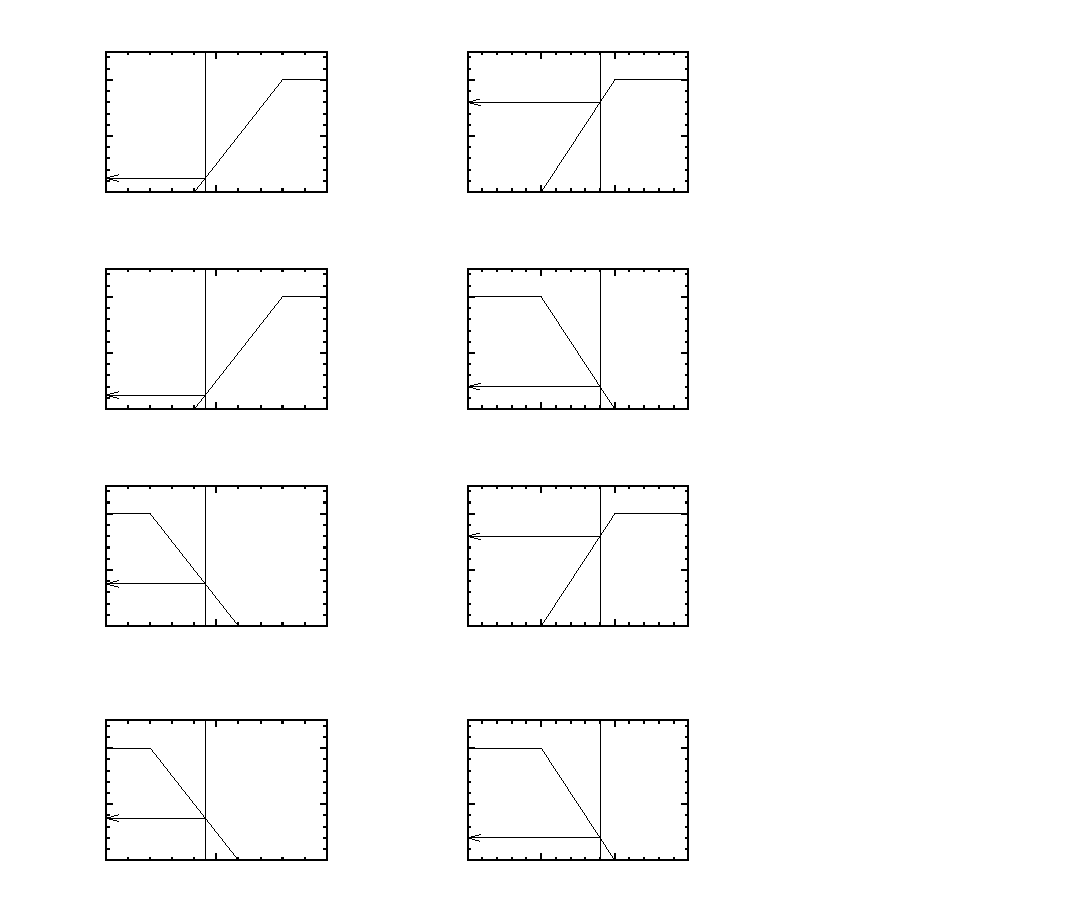
\includegraphics{deduction_of_system_output}}%
    \gplfronttext
  \end{picture}%
\endgroup

					\par\endgroup
			\end{minipage}}
		\end{center}
		\caption{Deduction of System Output}
	\end{figure}
%
	\begin{equation}
			y=	\frac{0.125\cdot(ax_{1}+bx_{2})+0.125\cdot(bx_{1}+cx_{2})+0.375\cdot(ex_{1}+fx_{2})+0.200\cdot(gx_{1}+hx_{2})}
					{(ax_{1}+bx_{2})+(bx_{1}+cx_{2})+(ex_{1}+fx_{2})+(gx_{1}+hx_{2})}
	\end{equation}
%	
\newpage
\subsection{Neural Networks}
One of the algorithms that are used in this thesis contains a derivative of an \gls{ANN}. That is why the basic foundations of \gls{ANN} are shortly described.\\
\indent Emulating the functionality of a human brain, \gls{ANN} are systems capable of learning. The multiple neurons that a network consists of exhibit the shape of nerve cells in a human brain. The basic functionality of one individual neuron, called perceptron, is illustrated in the figure below.
%
		\begin{figure}[H]
			\centering
				\setlength\fboxsep{5pt}
					\framebox{\input{perceptron.pdf_tex}}	
			\caption{Perceptron}
		\end{figure}
%
The perceptron's input ($x_{1}$,...,$x_{n}$), is rated with the weights ($w_{1}$,...,$w_{i}$). The sum of the rated inputs is afterwards computed and compared to a threshold ($\tau$). In case the summation exceeds the threshold value, the output function of the perceptron (f(z))is activated.
%
	\begin{equation}
			X=\sum\limits_{i=1}^{n}{x_{i}w_{i}};\,\,\,\,\,\,\, y=f(z)
	\end{equation}
%
The weight of the output is given by the output function (f).\\
A composition of multiple perceptrons (Fig. 2.10) leads to a neural network. It typically consists of one input layer to receive the inputs from the outside world and to redistribute them to all neurons of the hidden layer. Hidden layers detect the features of the input pattern and redirect them to the output layer that computes the system's output. In mathematical terms such a multi-layered feedforward network is a non-linear mapping from the input x on the output y.\\ 
During the training phase, the input pattern from a known data set is presented to the neural network. The resulting network's output is then compared to the training data output. The error between these two values is used to compute the changes in the weights in order to reduce the error.
%
\subsection{Adaptive Neuro Fuzzy Inference System}
In the previous sections, the basic principles of Fuzzy Logic and neural networks have been introduced. The combination of a FIS with a NN leads to so called \gls{HIS}. In general a \gls{HIS} combines at least two intelligent systems. 
The combination of Fuzzy Logic, neural networks and evolutionary algorithms forms the core of \gls{SC}. It is the emerging approach to build hybrid intelligent systems capable of reasoning and learning in uncertain and imprecise environments.\\
The \gls{ANFIS} is a \gls{HIS} which is part of the predictor that has been developed in this thesis. Its basic principles are therefore shortly described in the following section.
%
\subsubsection{Assembly of ANFIS}
The main idea of an \gls{ANFIS}, is to automatically derive a traceable model from implicit knowledge - hidden in a set of related input-output data - by means of a neural network.\\
The algorithm exhibits the shape of a six-layer feedforward neural network. In general, the algorithm can operate in two different modes. In the non-learning mode, it acts as a fuzzy inference system (section 2.3.1). In the learning mode it adapts its tuning parameters to a given data set. The learning operation results in extracting (n) fuzzy rules of the following shape:\\
%
	\begin{equation}
		\nonumber \text  {If $(x_1~is~A^{i}_{1},...,x_k~is~A^{i}_{k} )$}\text {~then 		}y=p^{i}_{0}+p^{i}_{1}x_{1}+...+p^{i}_{k}x_{k}
	\end{equation} 
%
from a given set of related input/output data, where (k) is the number of inputs.\\
The coefficients of the membership functions ($A^{1}_{1},...,A^{n}_{k}$) and the coefficients of the rule's consequences ($p^{1}_{0}$ to $p^{n}_{k}$) are tunable.\\
Fig. 2.11 illustrates the basic structure of an \gls{ANFIS} where two membership functions are related to each of the two inputs. (The number of inputs is set to two in order to reduce the complexity of the given example).
%
	\begin{figure}[H]
		\setlength\fboxsep{2pt}
		\fbox{%LaTeX with PSTricks extensions
%%Creator: 0.48.2
%%Please note this file requires PSTricks extensions
\psset{xunit=.5pt,yunit=.5pt,runit=.5pt}
\begin{pspicture}(744.09448242,1052.36218262)
{
\newrgbcolor{curcolor}{1 1 1}
\pscustom[linestyle=none,fillstyle=solid,fillcolor=curcolor]
{
\newpath
\moveto(135.6509552,1005.0186615)
\lineto(162.20447159,1005.0186615)
\lineto(162.20447159,979.90047073)
\lineto(135.6509552,979.90047073)
\closepath
}
}
{
\newrgbcolor{curcolor}{0 0 0}
\pscustom[linewidth=0.71044976,linecolor=curcolor]
{
\newpath
\moveto(135.6509552,1005.0186615)
\lineto(162.20447159,1005.0186615)
\lineto(162.20447159,979.90047073)
\lineto(135.6509552,979.90047073)
\closepath
}
}
{
\newrgbcolor{curcolor}{1 1 1}
\pscustom[linestyle=none,fillstyle=solid,fillcolor=curcolor]
{
\newpath
\moveto(257.80669223,992.4595704)
\curveto(257.80669223,985.22597819)(251.8152294,979.36199309)(244.42438544,979.36199309)
\curveto(237.03354149,979.36199309)(231.04207865,985.22597819)(231.04207865,992.4595704)
\curveto(231.04207865,999.69316261)(237.03354149,1005.55714772)(244.42438544,1005.55714772)
\curveto(251.8152294,1005.55714772)(257.80669223,999.69316261)(257.80669223,992.4595704)
\closepath
}
}
{
\newrgbcolor{curcolor}{0 0 0}
\pscustom[linewidth=0.56373651,linecolor=curcolor]
{
\newpath
\moveto(257.80669223,992.4595704)
\curveto(257.80669223,985.22597819)(251.8152294,979.36199309)(244.42438544,979.36199309)
\curveto(237.03354149,979.36199309)(231.04207865,985.22597819)(231.04207865,992.4595704)
\curveto(231.04207865,999.69316261)(237.03354149,1005.55714772)(244.42438544,1005.55714772)
\curveto(251.8152294,1005.55714772)(257.80669223,999.69316261)(257.80669223,992.4595704)
\closepath
}
}
{
\newrgbcolor{curcolor}{0 0 0}
\pscustom[linestyle=none,fillstyle=solid,fillcolor=curcolor]
{
\newpath
\moveto(141.6337738,989.42831421)
\lineto(145.48240662,999.44979858)
\lineto(146.91111755,999.44979858)
\lineto(151.01268005,989.42831421)
\lineto(149.50193787,989.42831421)
\lineto(148.33299255,992.46347046)
\lineto(144.14256287,992.46347046)
\lineto(143.04197693,989.42831421)
\closepath
\moveto(144.52537537,993.54354858)
\lineto(147.9228363,993.54354858)
\lineto(146.87693787,996.31893921)
\curveto(146.55792255,997.16203043)(146.32094362,997.85473807)(146.16600037,998.39706421)
\curveto(146.03839182,997.75447776)(145.85837897,997.11645756)(145.6259613,996.48300171)
\closepath
}
}
{
\newrgbcolor{curcolor}{0 0 0}
\pscustom[linestyle=none,fillstyle=solid,fillcolor=curcolor]
{
\newpath
\moveto(156.22166443,989.42831421)
\lineto(154.99119568,989.42831421)
\lineto(154.99119568,997.26913452)
\curveto(154.69496803,996.98657488)(154.30645931,996.70402308)(153.82566833,996.42147827)
\curveto(153.34487173,996.13891948)(152.91306877,995.92700563)(152.53025818,995.78573608)
\lineto(152.53025818,996.97518921)
\curveto(153.21840701,997.29874905)(153.81996891,997.69067574)(154.33494568,998.15097046)
\curveto(154.84991579,998.61124773)(155.21449876,999.05786187)(155.42869568,999.49081421)
\lineto(156.22166443,999.49081421)
\closepath
}
}
{
\newrgbcolor{curcolor}{1 1 1}
\pscustom[linestyle=none,fillstyle=solid,fillcolor=curcolor]
{
\newpath
\moveto(57.9213028,876.51403809)
\lineto(75.62035179,876.51403809)
\lineto(75.62035179,859.77169418)
\lineto(57.9213028,859.77169418)
\closepath
}
}
{
\newrgbcolor{curcolor}{0 0 0}
\pscustom[linewidth=0.47354499,linecolor=curcolor]
{
\newpath
\moveto(57.9213028,876.51403809)
\lineto(75.62035179,876.51403809)
\lineto(75.62035179,859.77169418)
\lineto(57.9213028,859.77169418)
\closepath
}
}
{
\newrgbcolor{curcolor}{1 1 1}
\pscustom[linestyle=none,fillstyle=solid,fillcolor=curcolor]
{
\newpath
\moveto(135.6509552,957.73036957)
\lineto(162.20447159,957.73036957)
\lineto(162.20447159,932.6121788)
\lineto(135.6509552,932.6121788)
\closepath
}
}
{
\newrgbcolor{curcolor}{0 0 0}
\pscustom[linewidth=0.71044976,linecolor=curcolor]
{
\newpath
\moveto(135.6509552,957.73036957)
\lineto(162.20447159,957.73036957)
\lineto(162.20447159,932.6121788)
\lineto(135.6509552,932.6121788)
\closepath
}
}
{
\newrgbcolor{curcolor}{1 1 1}
\pscustom[linestyle=none,fillstyle=solid,fillcolor=curcolor]
{
\newpath
\moveto(135.6509552,904.66069031)
\lineto(162.20447159,904.66069031)
\lineto(162.20447159,879.54249954)
\lineto(135.6509552,879.54249954)
\closepath
}
}
{
\newrgbcolor{curcolor}{0 0 0}
\pscustom[linewidth=0.71044976,linecolor=curcolor]
{
\newpath
\moveto(135.6509552,904.66069031)
\lineto(162.20447159,904.66069031)
\lineto(162.20447159,879.54249954)
\lineto(135.6509552,879.54249954)
\closepath
}
}
{
\newrgbcolor{curcolor}{1 1 1}
\pscustom[linestyle=none,fillstyle=solid,fillcolor=curcolor]
{
\newpath
\moveto(135.6509552,856.55909729)
\lineto(162.20447159,856.55909729)
\lineto(162.20447159,831.44090652)
\lineto(135.6509552,831.44090652)
\closepath
}
}
{
\newrgbcolor{curcolor}{0 0 0}
\pscustom[linewidth=0.71044976,linecolor=curcolor]
{
\newpath
\moveto(135.6509552,856.55909729)
\lineto(162.20447159,856.55909729)
\lineto(162.20447159,831.44090652)
\lineto(135.6509552,831.44090652)
\closepath
}
}
{
\newrgbcolor{curcolor}{1 1 1}
\pscustom[linestyle=none,fillstyle=solid,fillcolor=curcolor]
{
\newpath
\moveto(257.80669223,945.1712864)
\curveto(257.80669223,937.93769419)(251.8152294,932.07370909)(244.42438544,932.07370909)
\curveto(237.03354149,932.07370909)(231.04207865,937.93769419)(231.04207865,945.1712864)
\curveto(231.04207865,952.40487861)(237.03354149,958.26886372)(244.42438544,958.26886372)
\curveto(251.8152294,958.26886372)(257.80669223,952.40487861)(257.80669223,945.1712864)
\closepath
}
}
{
\newrgbcolor{curcolor}{0 0 0}
\pscustom[linewidth=0.56373651,linecolor=curcolor]
{
\newpath
\moveto(257.80669223,945.1712864)
\curveto(257.80669223,937.93769419)(251.8152294,932.07370909)(244.42438544,932.07370909)
\curveto(237.03354149,932.07370909)(231.04207865,937.93769419)(231.04207865,945.1712864)
\curveto(231.04207865,952.40487861)(237.03354149,958.26886372)(244.42438544,958.26886372)
\curveto(251.8152294,958.26886372)(257.80669223,952.40487861)(257.80669223,945.1712864)
\closepath
}
}
{
\newrgbcolor{curcolor}{1 1 1}
\pscustom[linestyle=none,fillstyle=solid,fillcolor=curcolor]
{
\newpath
\moveto(257.80669223,892.0678784)
\curveto(257.80669223,884.83428619)(251.8152294,878.97030109)(244.42438544,878.97030109)
\curveto(237.03354149,878.97030109)(231.04207865,884.83428619)(231.04207865,892.0678784)
\curveto(231.04207865,899.30147061)(237.03354149,905.16545572)(244.42438544,905.16545572)
\curveto(251.8152294,905.16545572)(257.80669223,899.30147061)(257.80669223,892.0678784)
\closepath
}
}
{
\newrgbcolor{curcolor}{0 0 0}
\pscustom[linewidth=0.56373651,linecolor=curcolor]
{
\newpath
\moveto(257.80669223,892.0678784)
\curveto(257.80669223,884.83428619)(251.8152294,878.97030109)(244.42438544,878.97030109)
\curveto(237.03354149,878.97030109)(231.04207865,884.83428619)(231.04207865,892.0678784)
\curveto(231.04207865,899.30147061)(237.03354149,905.16545572)(244.42438544,905.16545572)
\curveto(251.8152294,905.16545572)(257.80669223,899.30147061)(257.80669223,892.0678784)
\closepath
}
}
{
\newrgbcolor{curcolor}{1 1 1}
\pscustom[linestyle=none,fillstyle=solid,fillcolor=curcolor]
{
\newpath
\moveto(257.80669223,843.9999984)
\curveto(257.80669223,836.76640619)(251.8152294,830.90242109)(244.42438544,830.90242109)
\curveto(237.03354149,830.90242109)(231.04207865,836.76640619)(231.04207865,843.9999984)
\curveto(231.04207865,851.23359061)(237.03354149,857.09757572)(244.42438544,857.09757572)
\curveto(251.8152294,857.09757572)(257.80669223,851.23359061)(257.80669223,843.9999984)
\closepath
}
}
{
\newrgbcolor{curcolor}{0 0 0}
\pscustom[linewidth=0.56373651,linecolor=curcolor]
{
\newpath
\moveto(257.80669223,843.9999984)
\curveto(257.80669223,836.76640619)(251.8152294,830.90242109)(244.42438544,830.90242109)
\curveto(237.03354149,830.90242109)(231.04207865,836.76640619)(231.04207865,843.9999984)
\curveto(231.04207865,851.23359061)(237.03354149,857.09757572)(244.42438544,857.09757572)
\curveto(251.8152294,857.09757572)(257.80669223,851.23359061)(257.80669223,843.9999984)
\closepath
}
}
{
\newrgbcolor{curcolor}{1 1 1}
\pscustom[linestyle=none,fillstyle=solid,fillcolor=curcolor]
{
\newpath
\moveto(416.02516023,992.4595704)
\curveto(416.02516023,985.22597819)(410.0336974,979.36199309)(402.64285344,979.36199309)
\curveto(395.25200949,979.36199309)(389.26054665,985.22597819)(389.26054665,992.4595704)
\curveto(389.26054665,999.69316261)(395.25200949,1005.55714772)(402.64285344,1005.55714772)
\curveto(410.0336974,1005.55714772)(416.02516023,999.69316261)(416.02516023,992.4595704)
\closepath
}
}
{
\newrgbcolor{curcolor}{0 0 0}
\pscustom[linewidth=0.56373651,linecolor=curcolor]
{
\newpath
\moveto(416.02516023,992.4595704)
\curveto(416.02516023,985.22597819)(410.0336974,979.36199309)(402.64285344,979.36199309)
\curveto(395.25200949,979.36199309)(389.26054665,985.22597819)(389.26054665,992.4595704)
\curveto(389.26054665,999.69316261)(395.25200949,1005.55714772)(402.64285344,1005.55714772)
\curveto(410.0336974,1005.55714772)(416.02516023,999.69316261)(416.02516023,992.4595704)
\closepath
}
}
{
\newrgbcolor{curcolor}{1 1 1}
\pscustom[linestyle=none,fillstyle=solid,fillcolor=curcolor]
{
\newpath
\moveto(416.02516023,945.1712864)
\curveto(416.02516023,937.93769419)(410.0336974,932.07370909)(402.64285344,932.07370909)
\curveto(395.25200949,932.07370909)(389.26054665,937.93769419)(389.26054665,945.1712864)
\curveto(389.26054665,952.40487861)(395.25200949,958.26886372)(402.64285344,958.26886372)
\curveto(410.0336974,958.26886372)(416.02516023,952.40487861)(416.02516023,945.1712864)
\closepath
}
}
{
\newrgbcolor{curcolor}{0 0 0}
\pscustom[linewidth=0.56373651,linecolor=curcolor]
{
\newpath
\moveto(416.02516023,945.1712864)
\curveto(416.02516023,937.93769419)(410.0336974,932.07370909)(402.64285344,932.07370909)
\curveto(395.25200949,932.07370909)(389.26054665,937.93769419)(389.26054665,945.1712864)
\curveto(389.26054665,952.40487861)(395.25200949,958.26886372)(402.64285344,958.26886372)
\curveto(410.0336974,958.26886372)(416.02516023,952.40487861)(416.02516023,945.1712864)
\closepath
}
}
{
\newrgbcolor{curcolor}{1 1 1}
\pscustom[linestyle=none,fillstyle=solid,fillcolor=curcolor]
{
\newpath
\moveto(416.02516023,892.1015984)
\curveto(416.02516023,884.86800619)(410.0336974,879.00402109)(402.64285344,879.00402109)
\curveto(395.25200949,879.00402109)(389.26054665,884.86800619)(389.26054665,892.1015984)
\curveto(389.26054665,899.33519061)(395.25200949,905.19917572)(402.64285344,905.19917572)
\curveto(410.0336974,905.19917572)(416.02516023,899.33519061)(416.02516023,892.1015984)
\closepath
}
}
{
\newrgbcolor{curcolor}{0 0 0}
\pscustom[linewidth=0.56373651,linecolor=curcolor]
{
\newpath
\moveto(416.02516023,892.1015984)
\curveto(416.02516023,884.86800619)(410.0336974,879.00402109)(402.64285344,879.00402109)
\curveto(395.25200949,879.00402109)(389.26054665,884.86800619)(389.26054665,892.1015984)
\curveto(389.26054665,899.33519061)(395.25200949,905.19917572)(402.64285344,905.19917572)
\curveto(410.0336974,905.19917572)(416.02516023,899.33519061)(416.02516023,892.1015984)
\closepath
}
}
{
\newrgbcolor{curcolor}{1 1 1}
\pscustom[linestyle=none,fillstyle=solid,fillcolor=curcolor]
{
\newpath
\moveto(416.02516023,843.9999984)
\curveto(416.02516023,836.76640619)(410.0336974,830.90242109)(402.64285344,830.90242109)
\curveto(395.25200949,830.90242109)(389.26054665,836.76640619)(389.26054665,843.9999984)
\curveto(389.26054665,851.23359061)(395.25200949,857.09757572)(402.64285344,857.09757572)
\curveto(410.0336974,857.09757572)(416.02516023,851.23359061)(416.02516023,843.9999984)
\closepath
}
}
{
\newrgbcolor{curcolor}{0 0 0}
\pscustom[linewidth=0.56373651,linecolor=curcolor]
{
\newpath
\moveto(416.02516023,843.9999984)
\curveto(416.02516023,836.76640619)(410.0336974,830.90242109)(402.64285344,830.90242109)
\curveto(395.25200949,830.90242109)(389.26054665,836.76640619)(389.26054665,843.9999984)
\curveto(389.26054665,851.23359061)(395.25200949,857.09757572)(402.64285344,857.09757572)
\curveto(410.0336974,857.09757572)(416.02516023,851.23359061)(416.02516023,843.9999984)
\closepath
}
}
{
\newrgbcolor{curcolor}{1 1 1}
\pscustom[linestyle=none,fillstyle=solid,fillcolor=curcolor]
{
\newpath
\moveto(513.36608887,1005.0186615)
\lineto(539.91960526,1005.0186615)
\lineto(539.91960526,979.90047073)
\lineto(513.36608887,979.90047073)
\closepath
}
}
{
\newrgbcolor{curcolor}{0 0 0}
\pscustom[linewidth=0.71044976,linecolor=curcolor]
{
\newpath
\moveto(513.36608887,1005.0186615)
\lineto(539.91960526,1005.0186615)
\lineto(539.91960526,979.90047073)
\lineto(513.36608887,979.90047073)
\closepath
}
}
{
\newrgbcolor{curcolor}{1 1 1}
\pscustom[linestyle=none,fillstyle=solid,fillcolor=curcolor]
{
\newpath
\moveto(513.36608887,957.73036957)
\lineto(539.91960526,957.73036957)
\lineto(539.91960526,932.6121788)
\lineto(513.36608887,932.6121788)
\closepath
}
}
{
\newrgbcolor{curcolor}{0 0 0}
\pscustom[linewidth=0.71044976,linecolor=curcolor]
{
\newpath
\moveto(513.36608887,957.73036957)
\lineto(539.91960526,957.73036957)
\lineto(539.91960526,932.6121788)
\lineto(513.36608887,932.6121788)
\closepath
}
}
{
\newrgbcolor{curcolor}{1 1 1}
\pscustom[linestyle=none,fillstyle=solid,fillcolor=curcolor]
{
\newpath
\moveto(513.36608887,904.66069031)
\lineto(539.91960526,904.66069031)
\lineto(539.91960526,879.54249954)
\lineto(513.36608887,879.54249954)
\closepath
}
}
{
\newrgbcolor{curcolor}{0 0 0}
\pscustom[linewidth=0.71044976,linecolor=curcolor]
{
\newpath
\moveto(513.36608887,904.66069031)
\lineto(539.91960526,904.66069031)
\lineto(539.91960526,879.54249954)
\lineto(513.36608887,879.54249954)
\closepath
}
}
{
\newrgbcolor{curcolor}{1 1 1}
\pscustom[linestyle=none,fillstyle=solid,fillcolor=curcolor]
{
\newpath
\moveto(513.36608887,856.55909729)
\lineto(539.91960526,856.55909729)
\lineto(539.91960526,831.44090652)
\lineto(513.36608887,831.44090652)
\closepath
}
}
{
\newrgbcolor{curcolor}{0 0 0}
\pscustom[linewidth=0.71044976,linecolor=curcolor]
{
\newpath
\moveto(513.36608887,856.55909729)
\lineto(539.91960526,856.55909729)
\lineto(539.91960526,831.44090652)
\lineto(513.36608887,831.44090652)
\closepath
}
}
{
\newrgbcolor{curcolor}{0 0 0}
\pscustom[linestyle=none,fillstyle=solid,fillcolor=curcolor]
{
\newpath
\moveto(241.86383057,986.93612671)
\lineto(241.86383057,988.16659546)
\curveto(241.24859332,988.24406955)(240.74843106,988.38192749)(240.36334229,988.58016968)
\curveto(239.97824954,988.77841147)(239.64556758,989.09856088)(239.36529541,989.5406189)
\curveto(239.08502127,989.98267458)(238.92209825,990.52271311)(238.87652588,991.16073608)
\lineto(240.11383057,991.39315796)
\curveto(240.20953186,990.73234831)(240.37815148,990.24699724)(240.61968994,989.93710327)
\curveto(240.96604152,989.49960215)(241.38075465,989.25578729)(241.86383057,989.20565796)
\lineto(241.86383057,993.12265015)
\curveto(241.35796821,993.21834843)(240.84071612,993.41431178)(240.31207275,993.71054077)
\curveto(239.92014413,993.92928522)(239.61822386,994.23234481)(239.40631104,994.61972046)
\curveto(239.19439616,995.00708362)(239.08843923,995.44686183)(239.08843994,995.9390564)
\curveto(239.08843923,996.81404796)(239.39833475,997.52270611)(240.01812744,998.06503296)
\curveto(240.43283893,998.42960624)(241.04807269,998.65291331)(241.86383057,998.73495483)
\lineto(241.86383057,999.32284546)
\lineto(242.58843994,999.32284546)
\lineto(242.58843994,998.73495483)
\curveto(243.30392981,998.66658517)(243.87131205,998.45694996)(244.29058838,998.10604858)
\curveto(244.82834234,997.65942472)(245.15190973,997.0464696)(245.2612915,996.2671814)
\lineto(243.98980713,996.07577515)
\curveto(243.91688492,996.55883988)(243.76535513,996.92911946)(243.53521729,997.18661499)
\curveto(243.30506913,997.4440929)(242.989477,997.61385185)(242.58843994,997.69589233)
\lineto(242.58843994,994.14804077)
\curveto(243.20822678,993.99308724)(243.61838262,993.87231913)(243.81890869,993.78573608)
\curveto(244.20171537,993.61711105)(244.51388953,993.41203313)(244.75543213,993.17050171)
\curveto(244.99696197,992.9289607)(245.18267142,992.64185161)(245.31256104,992.30917358)
\curveto(245.44243678,991.97648769)(245.50737812,991.61646201)(245.50738525,991.22909546)
\curveto(245.50737812,990.37687992)(245.23621954,989.66594313)(244.69390869,989.09628296)
\curveto(244.15158521,988.52662135)(243.44976299,988.22128312)(242.58843994,988.18026733)
\lineto(242.58843994,986.93612671)
\closepath
\moveto(241.86383057,997.70956421)
\curveto(241.38531193,997.63663828)(241.00819643,997.44523223)(240.73248291,997.13534546)
\curveto(240.45676469,996.82544118)(240.31890675,996.45857957)(240.31890869,996.03475952)
\curveto(240.31890675,995.61548145)(240.43625689,995.26457034)(240.67095947,994.98202515)
\curveto(240.90565747,994.69946674)(241.30328077,994.47388103)(241.86383057,994.30526733)
\closepath
\moveto(242.58843994,989.20565796)
\curveto(243.06695088,989.26490186)(243.46229553,989.47225843)(243.7744751,989.82772827)
\curveto(244.08664387,990.18319522)(244.24273095,990.62297342)(244.24273682,991.14706421)
\curveto(244.24273095,991.59367558)(244.13221674,991.95256194)(243.91119385,992.22372437)
\curveto(243.69015989,992.4948791)(243.24924236,992.73755464)(242.58843994,992.95175171)
\closepath
}
}
{
\newrgbcolor{curcolor}{0 0 0}
\pscustom[linestyle=none,fillstyle=solid,fillcolor=curcolor]
{
\newpath
\moveto(249.07574463,988.20761108)
\lineto(246.17047119,998.57089233)
\lineto(247.16168213,998.57089233)
\lineto(250.06011963,988.20761108)
\closepath
}
}
{
\newrgbcolor{curcolor}{0 0 0}
\pscustom[linestyle=none,fillstyle=solid,fillcolor=curcolor]
{
\newpath
\moveto(250.97613525,985.59628296)
\lineto(250.97613525,995.63827515)
\lineto(252.097229,995.63827515)
\lineto(252.097229,994.69491577)
\curveto(252.36154961,995.06404971)(252.66005192,995.3409049)(252.99273682,995.52548218)
\curveto(253.32541584,995.71004516)(253.72873575,995.80233022)(254.20269775,995.80233765)
\curveto(254.82248465,995.80233022)(255.3693591,995.64282517)(255.84332275,995.32382202)
\curveto(256.31727482,995.00480498)(256.67502186,994.55477288)(256.91656494,993.97372437)
\curveto(257.15809429,993.39266466)(257.2788624,992.75578379)(257.27886963,992.06307983)
\curveto(257.2788624,991.32023835)(257.14556176,990.65145647)(256.87896729,990.05673218)
\curveto(256.61235916,989.46200453)(256.22498976,989.00627582)(255.71685791,988.68954468)
\curveto(255.20871473,988.37281291)(254.67437282,988.21444719)(254.11383057,988.21444702)
\curveto(253.70367067,988.21444719)(253.33566973,988.30103564)(253.00982666,988.47421265)
\curveto(252.68397768,988.64738946)(252.41623706,988.86613924)(252.206604,989.13046265)
\lineto(252.206604,985.59628296)
\closepath
\moveto(252.09039307,991.96737671)
\curveto(252.09039103,991.03312926)(252.27951844,990.34270027)(252.65777588,989.89608765)
\curveto(253.0360281,989.44947199)(253.49403546,989.22616492)(254.03179932,989.22616577)
\curveto(254.57866979,989.22616492)(255.04693104,989.45744724)(255.43658447,989.92001343)
\curveto(255.82622714,990.38257653)(256.02105116,991.09920993)(256.02105713,992.06991577)
\curveto(256.02105116,992.99504136)(255.83078442,993.687749)(255.45025635,994.14804077)
\curveto(255.06971748,994.608321)(254.61512809,994.838464)(254.08648682,994.83847046)
\curveto(253.56239477,994.838464)(253.0986908,994.59350982)(252.69537354,994.10360718)
\curveto(252.29205098,993.61369309)(252.09039103,992.90161698)(252.09039307,991.96737671)
\closepath
}
}
{
\newrgbcolor{curcolor}{0 0 0}
\pscustom[linestyle=none,fillstyle=solid,fillcolor=curcolor]
{
\newpath
\moveto(258.77593994,996.98495483)
\lineto(258.77593994,998.3999939)
\lineto(260.00640869,998.3999939)
\lineto(260.00640869,996.98495483)
\closepath
\moveto(258.77593994,988.37850952)
\lineto(258.77593994,995.63827515)
\lineto(260.00640869,995.63827515)
\lineto(260.00640869,988.37850952)
\closepath
}
}
{
\newrgbcolor{curcolor}{0 0 0}
\pscustom[linestyle=none,fillstyle=solid,fillcolor=curcolor]
{
\newpath
\moveto(264.44976807,986.93612671)
\lineto(264.44976807,988.16659546)
\curveto(263.83453082,988.24406955)(263.33436856,988.38192749)(262.94927979,988.58016968)
\curveto(262.56418704,988.77841147)(262.23150508,989.09856088)(261.95123291,989.5406189)
\curveto(261.67095877,989.98267458)(261.50803575,990.52271311)(261.46246338,991.16073608)
\lineto(262.69976807,991.39315796)
\curveto(262.79546936,990.73234831)(262.96408898,990.24699724)(263.20562744,989.93710327)
\curveto(263.55197902,989.49960215)(263.96669215,989.25578729)(264.44976807,989.20565796)
\lineto(264.44976807,993.12265015)
\curveto(263.94390571,993.21834843)(263.42665362,993.41431178)(262.89801025,993.71054077)
\curveto(262.50608163,993.92928522)(262.20416136,994.23234481)(261.99224854,994.61972046)
\curveto(261.78033366,995.00708362)(261.67437673,995.44686183)(261.67437744,995.9390564)
\curveto(261.67437673,996.81404796)(261.98427225,997.52270611)(262.60406494,998.06503296)
\curveto(263.01877643,998.42960624)(263.63401019,998.65291331)(264.44976807,998.73495483)
\lineto(264.44976807,999.32284546)
\lineto(265.17437744,999.32284546)
\lineto(265.17437744,998.73495483)
\curveto(265.88986731,998.66658517)(266.45724955,998.45694996)(266.87652588,998.10604858)
\curveto(267.41427984,997.65942472)(267.73784723,997.0464696)(267.847229,996.2671814)
\lineto(266.57574463,996.07577515)
\curveto(266.50282242,996.55883988)(266.35129263,996.92911946)(266.12115479,997.18661499)
\curveto(265.89100663,997.4440929)(265.5754145,997.61385185)(265.17437744,997.69589233)
\lineto(265.17437744,994.14804077)
\curveto(265.79416428,993.99308724)(266.20432012,993.87231913)(266.40484619,993.78573608)
\curveto(266.78765287,993.61711105)(267.09982703,993.41203313)(267.34136963,993.17050171)
\curveto(267.58289947,992.9289607)(267.76860892,992.64185161)(267.89849854,992.30917358)
\curveto(268.02837428,991.97648769)(268.09331562,991.61646201)(268.09332275,991.22909546)
\curveto(268.09331562,990.37687992)(267.82215704,989.66594313)(267.27984619,989.09628296)
\curveto(266.73752271,988.52662135)(266.03570049,988.22128312)(265.17437744,988.18026733)
\lineto(265.17437744,986.93612671)
\closepath
\moveto(264.44976807,997.70956421)
\curveto(263.97124943,997.63663828)(263.59413393,997.44523223)(263.31842041,997.13534546)
\curveto(263.04270219,996.82544118)(262.90484425,996.45857957)(262.90484619,996.03475952)
\curveto(262.90484425,995.61548145)(263.02219439,995.26457034)(263.25689697,994.98202515)
\curveto(263.49159497,994.69946674)(263.88921827,994.47388103)(264.44976807,994.30526733)
\closepath
\moveto(265.17437744,989.20565796)
\curveto(265.65288838,989.26490186)(266.04823303,989.47225843)(266.3604126,989.82772827)
\curveto(266.67258137,990.18319522)(266.82866845,990.62297342)(266.82867432,991.14706421)
\curveto(266.82866845,991.59367558)(266.71815424,991.95256194)(266.49713135,992.22372437)
\curveto(266.27609739,992.4948791)(265.83517986,992.73755464)(265.17437744,992.95175171)
\closepath
}
}
{
\newrgbcolor{curcolor}{0 0 0}
\pscustom[linestyle=none,fillstyle=solid,fillcolor=curcolor]
{
\newpath
\moveto(273.972229,988.37850952)
\lineto(272.74176025,988.37850952)
\lineto(272.74176025,996.21932983)
\curveto(272.44553261,995.93677019)(272.05702388,995.65421839)(271.57623291,995.37167358)
\curveto(271.0954363,995.08911479)(270.66363335,994.87720094)(270.28082275,994.7359314)
\lineto(270.28082275,995.92538452)
\curveto(270.96897158,996.24894436)(271.57053348,996.64087105)(272.08551025,997.10116577)
\curveto(272.60048037,997.56144305)(272.96506334,998.00805718)(273.17926025,998.44100952)
\lineto(273.972229,998.44100952)
\closepath
}
}
{
\newrgbcolor{curcolor}{0 0 0}
\pscustom[linestyle=none,fillstyle=solid,fillcolor=curcolor]
{
\newpath
\moveto(397.509552,987.42832184)
\lineto(397.509552,997.44980621)
\lineto(398.86990356,997.44980621)
\lineto(404.13357544,989.58164215)
\lineto(404.13357544,997.44980621)
\lineto(405.40505981,997.44980621)
\lineto(405.40505981,987.42832184)
\lineto(404.04470825,987.42832184)
\lineto(398.78103638,995.30332184)
\lineto(398.78103638,987.42832184)
\closepath
}
}
{
\newrgbcolor{curcolor}{0 0 0}
\pscustom[linestyle=none,fillstyle=solid,fillcolor=curcolor]
{
\newpath
\moveto(411.77615356,987.42832184)
\lineto(410.54568481,987.42832184)
\lineto(410.54568481,995.26914215)
\curveto(410.24945717,994.98658251)(409.86094844,994.70403071)(409.38015747,994.4214859)
\curveto(408.89936086,994.13892711)(408.46755791,993.92701326)(408.08474731,993.78574371)
\lineto(408.08474731,994.97519684)
\curveto(408.77289614,995.29875668)(409.37445804,995.69068337)(409.88943481,996.15097809)
\curveto(410.40440493,996.61125536)(410.7689879,997.0578695)(410.98318481,997.49082184)
\lineto(411.77615356,997.49082184)
\closepath
}
}
{
\newrgbcolor{curcolor}{0 0 0}
\pscustom[linestyle=none,fillstyle=solid,fillcolor=curcolor]
{
\newpath
\moveto(528.29858398,987.42831421)
\lineto(527.06811523,987.42831421)
\lineto(527.06811523,995.26913452)
\curveto(526.77188759,994.98657488)(526.38337886,994.70402308)(525.90258789,994.42147827)
\curveto(525.42179128,994.13891948)(524.98998833,993.92700563)(524.60717773,993.78573608)
\lineto(524.60717773,994.97518921)
\curveto(525.29532656,995.29874905)(525.89688846,995.69067574)(526.41186523,996.15097046)
\curveto(526.92683535,996.61124773)(527.29141832,997.05786187)(527.50561523,997.49081421)
\lineto(528.29858398,997.49081421)
\closepath
}
}
{
\newrgbcolor{curcolor}{0 0 0}
\pscustom[linestyle=none,fillstyle=solid,fillcolor=curcolor]
{
\newpath
\moveto(396.59353638,940.14002991)
\lineto(396.59353638,950.16151428)
\lineto(397.95388794,950.16151428)
\lineto(403.21755981,942.29335022)
\lineto(403.21755981,950.16151428)
\lineto(404.48904419,950.16151428)
\lineto(404.48904419,940.14002991)
\lineto(403.12869263,940.14002991)
\lineto(397.86502075,948.01502991)
\lineto(397.86502075,940.14002991)
\closepath
}
}
{
\newrgbcolor{curcolor}{0 0 0}
\pscustom[linestyle=none,fillstyle=solid,fillcolor=curcolor]
{
\newpath
\moveto(412.69216919,941.32264709)
\lineto(412.69216919,940.14002991)
\lineto(406.06814575,940.14002991)
\curveto(406.05903075,940.43625357)(406.10688227,940.72108401)(406.21170044,940.99452209)
\curveto(406.3803195,941.44569266)(406.65033876,941.89002816)(407.02175903,942.32752991)
\curveto(407.39317656,942.76502728)(407.92979711,943.27088615)(408.63162231,943.84510803)
\curveto(409.72081095,944.7383326)(410.45681281,945.44585142)(410.83963013,945.96766663)
\curveto(411.22243705,946.48947017)(411.41384311,946.9827965)(411.41384888,947.44764709)
\curveto(411.41384311,947.93526951)(411.23952688,948.34656467)(410.89089966,948.68153381)
\curveto(410.54226195,949.01648587)(410.08767256,949.18396618)(409.52713013,949.18397522)
\curveto(408.93467892,949.18396618)(408.46072106,949.00623198)(408.10525513,948.65077209)
\curveto(407.74978427,948.29529519)(407.56977143,947.80310818)(407.56521606,947.17420959)
\lineto(406.30056763,947.30409241)
\curveto(406.38715543,948.24744367)(406.71300145,948.96635572)(407.27810669,949.46083069)
\curveto(407.84320866,949.95528702)(408.60199696,950.20251984)(409.55447388,950.20252991)
\curveto(410.51605755,950.20251984)(411.27712449,949.93591855)(411.837677,949.40272522)
\curveto(412.39821712,948.86951337)(412.67849028,948.20870673)(412.67849731,947.42030334)
\curveto(412.67849028,947.0192548)(412.59645911,946.62504946)(412.43240356,946.23768616)
\curveto(412.26833444,945.85031066)(411.99603654,945.44243346)(411.61550903,945.01405334)
\curveto(411.23496959,944.58566348)(410.602646,943.99777345)(409.71853638,943.25038147)
\curveto(408.98025179,942.63058731)(408.50629393,942.21017758)(408.29666138,941.989151)
\curveto(408.08702352,941.76812073)(407.91384661,941.54595298)(407.77713013,941.32264709)
\closepath
}
}
{
\newrgbcolor{curcolor}{0 0 0}
\pscustom[linestyle=none,fillstyle=solid,fillcolor=curcolor]
{
\newpath
\moveto(396.54226685,887.15921021)
\lineto(396.54226685,897.18069458)
\lineto(397.90261841,897.18069458)
\lineto(403.16629028,889.31253052)
\lineto(403.16629028,897.18069458)
\lineto(404.43777466,897.18069458)
\lineto(404.43777466,887.15921021)
\lineto(403.0774231,887.15921021)
\lineto(397.81375122,895.03421021)
\lineto(397.81375122,887.15921021)
\closepath
}
}
{
\newrgbcolor{curcolor}{0 0 0}
\pscustom[linestyle=none,fillstyle=solid,fillcolor=curcolor]
{
\newpath
\moveto(406.18093872,889.80471802)
\lineto(407.41140747,889.96878052)
\curveto(407.55268155,889.27151278)(407.79307845,888.76907188)(408.13259888,888.4614563)
\curveto(408.47211423,888.15383812)(408.88568803,888.00002968)(409.37332153,888.00003052)
\curveto(409.95209322,888.00002968)(410.44086226,888.20055031)(410.83963013,888.60159302)
\curveto(411.2383875,889.00263284)(411.43776881,889.49937714)(411.43777466,890.09182739)
\curveto(411.43776881,890.65692806)(411.25319869,891.12291067)(410.88406372,891.48977661)
\curveto(410.51491817,891.85663389)(410.0455176,892.0400647)(409.4758606,892.04006958)
\curveto(409.24343507,892.0400647)(408.95404734,891.99449183)(408.60769653,891.90335083)
\lineto(408.74441528,892.98342896)
\curveto(408.8264433,892.97430856)(408.89252396,892.96975127)(408.94265747,892.96975708)
\curveto(409.46674214,892.96975127)(409.93842135,893.10646988)(410.35769653,893.37991333)
\curveto(410.77696218,893.65334434)(410.98659739,894.07489339)(410.98660278,894.64456177)
\curveto(410.98659739,895.09572571)(410.83392827,895.46942325)(410.52859497,895.76565552)
\curveto(410.2232518,896.06187057)(409.82904646,896.2099824)(409.34597778,896.20999146)
\curveto(408.86745888,896.2099824)(408.46869626,896.05959193)(408.14968872,895.75881958)
\curveto(407.83067607,895.45803003)(407.62559815,895.00685861)(407.53445435,894.40530396)
\lineto(406.3039856,894.62405396)
\curveto(406.45437536,895.44891546)(406.79617189,896.08807497)(407.32937622,896.54153442)
\curveto(407.86257708,896.99497511)(408.52566235,897.22170014)(409.31863403,897.22171021)
\curveto(409.86550476,897.22170014)(410.36908499,897.10435)(410.82937622,896.86965942)
\curveto(411.28965698,896.63494943)(411.64170741,896.31480001)(411.88552856,895.90921021)
\curveto(412.12933713,895.5036029)(412.25124456,895.07293927)(412.25125122,894.61721802)
\curveto(412.25124456,894.18426828)(412.13503374,893.79006295)(411.90261841,893.43460083)
\curveto(411.67019046,893.07912616)(411.32611528,892.79657436)(410.87039185,892.58694458)
\curveto(411.46283389,892.45022054)(411.92311989,892.16652942)(412.25125122,891.73587036)
\curveto(412.57936923,891.30520215)(412.74343157,890.76630295)(412.74343872,890.11917114)
\curveto(412.74343157,889.24416906)(412.42442147,888.50247058)(411.78640747,887.89407349)
\curveto(411.14838108,887.28567492)(410.34174126,886.98147601)(409.3664856,886.98147583)
\curveto(408.48692541,886.98147601)(407.75662015,887.24352002)(407.17556763,887.76760864)
\curveto(406.59451194,888.29169605)(406.2629693,888.97073183)(406.18093872,889.80471802)
\closepath
}
}
{
\newrgbcolor{curcolor}{0 0 0}
\pscustom[linestyle=none,fillstyle=solid,fillcolor=curcolor]
{
\newpath
\moveto(396.56277466,838.98925781)
\lineto(396.56277466,849.01074219)
\lineto(397.92312622,849.01074219)
\lineto(403.1867981,841.14257812)
\lineto(403.1867981,849.01074219)
\lineto(404.45828247,849.01074219)
\lineto(404.45828247,838.98925781)
\lineto(403.09793091,838.98925781)
\lineto(397.83425903,846.86425781)
\lineto(397.83425903,838.98925781)
\closepath
}
}
{
\newrgbcolor{curcolor}{0 0 0}
\pscustom[linestyle=none,fillstyle=solid,fillcolor=curcolor]
{
\newpath
\moveto(410.13894653,838.98925781)
\lineto(410.13894653,841.38867188)
\lineto(405.79129028,841.38867188)
\lineto(405.79129028,842.51660156)
\lineto(410.36453247,849.01074219)
\lineto(411.36941528,849.01074219)
\lineto(411.36941528,842.51660156)
\lineto(412.72293091,842.51660156)
\lineto(412.72293091,841.38867188)
\lineto(411.36941528,841.38867188)
\lineto(411.36941528,838.98925781)
\closepath
\moveto(410.13894653,842.51660156)
\lineto(410.13894653,847.03515625)
\lineto(407.00125122,842.51660156)
\closepath
}
}
{
\newrgbcolor{curcolor}{0 0 0}
\pscustom[linestyle=none,fillstyle=solid,fillcolor=curcolor]
{
\newpath
\moveto(242.94781494,939.64784241)
\lineto(242.94781494,940.87831116)
\curveto(242.3325777,940.95578525)(241.83241544,941.09364319)(241.44732666,941.29188538)
\curveto(241.06223391,941.49012716)(240.72955195,941.81027658)(240.44927979,942.25233459)
\curveto(240.16900564,942.69439028)(240.00608263,943.2344288)(239.96051025,943.87245178)
\lineto(241.19781494,944.10487366)
\curveto(241.29351623,943.44406401)(241.46213586,942.95871293)(241.70367432,942.64881897)
\curveto(242.05002589,942.21131785)(242.46473902,941.96750299)(242.94781494,941.91737366)
\lineto(242.94781494,945.83436584)
\curveto(242.44195259,945.93006413)(241.9247005,946.12602748)(241.39605713,946.42225647)
\curveto(241.0041285,946.64100092)(240.70220823,946.94406051)(240.49029541,947.33143616)
\curveto(240.27838053,947.71879932)(240.17242361,948.15857753)(240.17242432,948.65077209)
\curveto(240.17242361,949.52576366)(240.48231913,950.2344218)(241.10211182,950.77674866)
\curveto(241.5168233,951.14132194)(242.13205706,951.36462901)(242.94781494,951.44667053)
\lineto(242.94781494,952.03456116)
\lineto(243.67242432,952.03456116)
\lineto(243.67242432,951.44667053)
\curveto(244.38791418,951.37830087)(244.95529643,951.16866566)(245.37457275,950.81776428)
\curveto(245.91232672,950.37114042)(246.2358941,949.7581853)(246.34527588,948.97889709)
\lineto(245.0737915,948.78749084)
\curveto(245.0008693,949.27055558)(244.8493395,949.64083516)(244.61920166,949.89833069)
\curveto(244.3890535,950.1558086)(244.07346137,950.32556755)(243.67242432,950.40760803)
\lineto(243.67242432,946.85975647)
\curveto(244.29221115,946.70480294)(244.70236699,946.58403483)(244.90289307,946.49745178)
\curveto(245.28569974,946.32882675)(245.59787391,946.12374883)(245.8394165,945.88221741)
\curveto(246.08094634,945.6406764)(246.26665579,945.35356731)(246.39654541,945.02088928)
\curveto(246.52642116,944.68820339)(246.5913625,944.32817771)(246.59136963,943.94081116)
\curveto(246.5913625,943.08859562)(246.32020392,942.37765883)(245.77789307,941.80799866)
\curveto(245.23556958,941.23833705)(244.53374737,940.93299881)(243.67242432,940.89198303)
\lineto(243.67242432,939.64784241)
\closepath
\moveto(242.94781494,950.42127991)
\curveto(242.46929631,950.34835398)(242.0921808,950.15694792)(241.81646729,949.84706116)
\curveto(241.54074906,949.53715688)(241.40289112,949.17029526)(241.40289307,948.74647522)
\curveto(241.40289112,948.32719715)(241.52024127,947.97628604)(241.75494385,947.69374084)
\curveto(241.98964184,947.41118244)(242.38726514,947.18559673)(242.94781494,947.01698303)
\closepath
\moveto(243.67242432,941.91737366)
\curveto(244.15093525,941.97661756)(244.54627991,942.18397413)(244.85845947,942.53944397)
\curveto(245.17062824,942.89491092)(245.32671533,943.33468912)(245.32672119,943.85877991)
\curveto(245.32671533,944.30539128)(245.21620111,944.66427764)(244.99517822,944.93544006)
\curveto(244.77414426,945.2065948)(244.33322674,945.44927034)(243.67242432,945.66346741)
\closepath
}
}
{
\newrgbcolor{curcolor}{0 0 0}
\pscustom[linestyle=none,fillstyle=solid,fillcolor=curcolor]
{
\newpath
\moveto(250.159729,940.91932678)
\lineto(247.25445557,951.28260803)
\lineto(248.2456665,951.28260803)
\lineto(251.144104,940.91932678)
\closepath
}
}
{
\newrgbcolor{curcolor}{0 0 0}
\pscustom[linestyle=none,fillstyle=solid,fillcolor=curcolor]
{
\newpath
\moveto(252.06011963,938.30799866)
\lineto(252.06011963,948.34999084)
\lineto(253.18121338,948.34999084)
\lineto(253.18121338,947.40663147)
\curveto(253.44553399,947.77576541)(253.74403629,948.0526206)(254.07672119,948.23719788)
\curveto(254.40940021,948.42176086)(254.81272012,948.51404592)(255.28668213,948.51405334)
\curveto(255.90646903,948.51404592)(256.45334348,948.35454087)(256.92730713,948.03553772)
\curveto(257.4012592,947.71652068)(257.75900624,947.26648857)(258.00054932,946.68544006)
\curveto(258.24207867,946.10438036)(258.36284678,945.46749949)(258.362854,944.77479553)
\curveto(258.36284678,944.03195405)(258.22954613,943.36317217)(257.96295166,942.76844788)
\curveto(257.69634354,942.17372023)(257.30897413,941.71799152)(256.80084229,941.40126038)
\curveto(256.29269911,941.08452861)(255.7583572,940.92616288)(255.19781494,940.92616272)
\curveto(254.78765504,940.92616288)(254.41965411,941.01275134)(254.09381104,941.18592834)
\curveto(253.76796205,941.35910516)(253.50022143,941.57785494)(253.29058838,941.84217834)
\lineto(253.29058838,938.30799866)
\closepath
\moveto(253.17437744,944.67909241)
\curveto(253.1743754,943.74484496)(253.36350282,943.05441596)(253.74176025,942.60780334)
\curveto(254.12001248,942.16118769)(254.57801983,941.93788062)(255.11578369,941.93788147)
\curveto(255.66265417,941.93788062)(256.13091542,942.16916294)(256.52056885,942.63172913)
\curveto(256.91021151,943.09429223)(257.10503554,943.81092562)(257.1050415,944.78163147)
\curveto(257.10503554,945.70675706)(256.9147688,946.3994647)(256.53424072,946.85975647)
\curveto(256.15370185,947.3200367)(255.69911246,947.5501797)(255.17047119,947.55018616)
\curveto(254.64637914,947.5501797)(254.18267518,947.30522552)(253.77935791,946.81532288)
\curveto(253.37603536,946.32540879)(253.1743754,945.61333268)(253.17437744,944.67909241)
\closepath
}
}
{
\newrgbcolor{curcolor}{0 0 0}
\pscustom[linestyle=none,fillstyle=solid,fillcolor=curcolor]
{
\newpath
\moveto(259.85992432,949.69667053)
\lineto(259.85992432,951.11170959)
\lineto(261.09039307,951.11170959)
\lineto(261.09039307,949.69667053)
\closepath
\moveto(259.85992432,941.09022522)
\lineto(259.85992432,948.34999084)
\lineto(261.09039307,948.34999084)
\lineto(261.09039307,941.09022522)
\closepath
}
}
{
\newrgbcolor{curcolor}{0 0 0}
\pscustom[linestyle=none,fillstyle=solid,fillcolor=curcolor]
{
\newpath
\moveto(265.53375244,939.64784241)
\lineto(265.53375244,940.87831116)
\curveto(264.9185152,940.95578525)(264.41835294,941.09364319)(264.03326416,941.29188538)
\curveto(263.64817141,941.49012716)(263.31548945,941.81027658)(263.03521729,942.25233459)
\curveto(262.75494314,942.69439028)(262.59202013,943.2344288)(262.54644775,943.87245178)
\lineto(263.78375244,944.10487366)
\curveto(263.87945373,943.44406401)(264.04807336,942.95871293)(264.28961182,942.64881897)
\curveto(264.63596339,942.21131785)(265.05067652,941.96750299)(265.53375244,941.91737366)
\lineto(265.53375244,945.83436584)
\curveto(265.02789009,945.93006413)(264.510638,946.12602748)(263.98199463,946.42225647)
\curveto(263.590066,946.64100092)(263.28814573,946.94406051)(263.07623291,947.33143616)
\curveto(262.86431803,947.71879932)(262.75836111,948.15857753)(262.75836182,948.65077209)
\curveto(262.75836111,949.52576366)(263.06825663,950.2344218)(263.68804932,950.77674866)
\curveto(264.1027608,951.14132194)(264.71799456,951.36462901)(265.53375244,951.44667053)
\lineto(265.53375244,952.03456116)
\lineto(266.25836182,952.03456116)
\lineto(266.25836182,951.44667053)
\curveto(266.97385168,951.37830087)(267.54123393,951.16866566)(267.96051025,950.81776428)
\curveto(268.49826422,950.37114042)(268.8218316,949.7581853)(268.93121338,948.97889709)
\lineto(267.659729,948.78749084)
\curveto(267.5868068,949.27055558)(267.435277,949.64083516)(267.20513916,949.89833069)
\curveto(266.974991,950.1558086)(266.65939887,950.32556755)(266.25836182,950.40760803)
\lineto(266.25836182,946.85975647)
\curveto(266.87814865,946.70480294)(267.28830449,946.58403483)(267.48883057,946.49745178)
\curveto(267.87163724,946.32882675)(268.18381141,946.12374883)(268.425354,945.88221741)
\curveto(268.66688384,945.6406764)(268.85259329,945.35356731)(268.98248291,945.02088928)
\curveto(269.11235866,944.68820339)(269.1773,944.32817771)(269.17730713,943.94081116)
\curveto(269.1773,943.08859562)(268.90614142,942.37765883)(268.36383057,941.80799866)
\curveto(267.82150708,941.23833705)(267.11968487,940.93299881)(266.25836182,940.89198303)
\lineto(266.25836182,939.64784241)
\closepath
\moveto(265.53375244,950.42127991)
\curveto(265.05523381,950.34835398)(264.6781183,950.15694792)(264.40240479,949.84706116)
\curveto(264.12668656,949.53715688)(263.98882862,949.17029526)(263.98883057,948.74647522)
\curveto(263.98882862,948.32719715)(264.10617877,947.97628604)(264.34088135,947.69374084)
\curveto(264.57557934,947.41118244)(264.97320264,947.18559673)(265.53375244,947.01698303)
\closepath
\moveto(266.25836182,941.91737366)
\curveto(266.73687275,941.97661756)(267.13221741,942.18397413)(267.44439697,942.53944397)
\curveto(267.75656574,942.89491092)(267.91265283,943.33468912)(267.91265869,943.85877991)
\curveto(267.91265283,944.30539128)(267.80213861,944.66427764)(267.58111572,944.93544006)
\curveto(267.36008176,945.2065948)(266.91916424,945.44927034)(266.25836182,945.66346741)
\closepath
}
}
{
\newrgbcolor{curcolor}{0 0 0}
\pscustom[linestyle=none,fillstyle=solid,fillcolor=curcolor]
{
\newpath
\moveto(276.88824463,942.27284241)
\lineto(276.88824463,941.09022522)
\lineto(270.26422119,941.09022522)
\curveto(270.25510619,941.38644888)(270.30295771,941.67127933)(270.40777588,941.94471741)
\curveto(270.57639493,942.39588798)(270.8464142,942.84022347)(271.21783447,943.27772522)
\curveto(271.58925199,943.71522259)(272.12587255,944.22108146)(272.82769775,944.79530334)
\curveto(273.91688639,945.68852791)(274.65288825,946.39604674)(275.03570557,946.91786194)
\curveto(275.41851249,947.43966548)(275.60991855,947.93299181)(275.60992432,948.39784241)
\curveto(275.60991855,948.88546482)(275.43560231,949.29675998)(275.0869751,949.63172913)
\curveto(274.73833739,949.96668119)(274.283748,950.13416149)(273.72320557,950.13417053)
\curveto(273.13075436,950.13416149)(272.6567965,949.95642729)(272.30133057,949.60096741)
\curveto(271.94585971,949.2454905)(271.76584687,948.75330349)(271.7612915,948.12440491)
\lineto(270.49664307,948.25428772)
\curveto(270.58323087,949.19763899)(270.90907689,949.91655103)(271.47418213,950.411026)
\curveto(272.0392841,950.90548233)(272.7980724,951.15271516)(273.75054932,951.15272522)
\curveto(274.71213299,951.15271516)(275.47319993,950.88611386)(276.03375244,950.35292053)
\curveto(276.59429256,949.81970868)(276.87456572,949.15890205)(276.87457275,948.37049866)
\curveto(276.87456572,947.96945011)(276.79253455,947.57524478)(276.628479,947.18788147)
\curveto(276.46440988,946.80050597)(276.19211198,946.39262877)(275.81158447,945.96424866)
\curveto(275.43104503,945.53585879)(274.79872144,944.94796876)(273.91461182,944.20057678)
\curveto(273.17632723,943.58078262)(272.70236937,943.16037289)(272.49273682,942.93934631)
\curveto(272.28309896,942.71831604)(272.10992205,942.49614829)(271.97320557,942.27284241)
\closepath
}
}
{
\newrgbcolor{curcolor}{0 0 0}
\pscustom[linestyle=none,fillstyle=solid,fillcolor=curcolor]
{
\newpath
\moveto(242.89654541,886.54443359)
\lineto(242.89654541,887.77490234)
\curveto(242.28130816,887.85237644)(241.7811459,887.99023437)(241.39605713,888.18847656)
\curveto(241.01096438,888.38671835)(240.67828242,888.70686777)(240.39801025,889.14892578)
\curveto(240.11773611,889.59098147)(239.95481309,890.13101999)(239.90924072,890.76904297)
\lineto(241.14654541,891.00146484)
\curveto(241.2422467,890.3406552)(241.41086633,889.85530412)(241.65240479,889.54541016)
\curveto(241.99875636,889.10790904)(242.41346949,888.86409417)(242.89654541,888.81396484)
\lineto(242.89654541,892.73095703)
\curveto(242.39068305,892.82665532)(241.87343097,893.02261866)(241.3447876,893.31884766)
\curveto(240.95285897,893.53759211)(240.6509387,893.8406517)(240.43902588,894.22802734)
\curveto(240.227111,894.61539051)(240.12115407,895.05516871)(240.12115479,895.54736328)
\curveto(240.12115407,896.42235485)(240.4310496,897.13101299)(241.05084229,897.67333984)
\curveto(241.46555377,898.03791313)(242.08078753,898.26122019)(242.89654541,898.34326172)
\lineto(242.89654541,898.93115234)
\lineto(243.62115479,898.93115234)
\lineto(243.62115479,898.34326172)
\curveto(244.33664465,898.27489206)(244.9040269,898.06525685)(245.32330322,897.71435547)
\curveto(245.86105719,897.2677316)(246.18462457,896.65477649)(246.29400635,895.87548828)
\lineto(245.02252197,895.68408203)
\curveto(244.94959977,896.16714677)(244.79806997,896.53742635)(244.56793213,896.79492188)
\curveto(244.33778397,897.05239979)(244.02219184,897.22215873)(243.62115479,897.30419922)
\lineto(243.62115479,893.75634766)
\curveto(244.24094162,893.60139413)(244.65109746,893.48062602)(244.85162354,893.39404297)
\curveto(245.23443021,893.22541794)(245.54660438,893.02034002)(245.78814697,892.77880859)
\curveto(246.02967681,892.53726758)(246.21538626,892.2501585)(246.34527588,891.91748047)
\curveto(246.47515163,891.58479458)(246.54009297,891.2247689)(246.5401001,890.83740234)
\curveto(246.54009297,889.9851868)(246.26893438,889.27425001)(245.72662354,888.70458984)
\curveto(245.18430005,888.13492824)(244.48247784,887.82959)(243.62115479,887.78857422)
\lineto(243.62115479,886.54443359)
\closepath
\moveto(242.89654541,897.31787109)
\curveto(242.41802678,897.24494517)(242.04091127,897.05353911)(241.76519775,896.74365234)
\curveto(241.48947953,896.43374806)(241.35162159,896.06688645)(241.35162354,895.64306641)
\curveto(241.35162159,895.22378834)(241.46897174,894.87287723)(241.70367432,894.59033203)
\curveto(241.93837231,894.30777363)(242.33599561,894.08218792)(242.89654541,893.91357422)
\closepath
\moveto(243.62115479,888.81396484)
\curveto(244.09966572,888.87320875)(244.49501038,889.08056531)(244.80718994,889.43603516)
\curveto(245.11935871,889.7915021)(245.27544579,890.23128031)(245.27545166,890.75537109)
\curveto(245.27544579,891.20198246)(245.16493158,891.56086882)(244.94390869,891.83203125)
\curveto(244.72287473,892.10318599)(244.28195721,892.34586153)(243.62115479,892.56005859)
\closepath
}
}
{
\newrgbcolor{curcolor}{0 0 0}
\pscustom[linestyle=none,fillstyle=solid,fillcolor=curcolor]
{
\newpath
\moveto(250.10845947,887.81591797)
\lineto(247.20318604,898.17919922)
\lineto(248.19439697,898.17919922)
\lineto(251.09283447,887.81591797)
\closepath
}
}
{
\newrgbcolor{curcolor}{0 0 0}
\pscustom[linestyle=none,fillstyle=solid,fillcolor=curcolor]
{
\newpath
\moveto(252.0088501,885.20458984)
\lineto(252.0088501,895.24658203)
\lineto(253.12994385,895.24658203)
\lineto(253.12994385,894.30322266)
\curveto(253.39426446,894.6723566)(253.69276676,894.94921179)(254.02545166,895.13378906)
\curveto(254.35813068,895.31835204)(254.76145059,895.41063711)(255.2354126,895.41064453)
\curveto(255.8551995,895.41063711)(256.40207395,895.25113206)(256.8760376,894.93212891)
\curveto(257.34998967,894.61311186)(257.70773671,894.16307976)(257.94927979,893.58203125)
\curveto(258.19080914,893.00097155)(258.31157725,892.36409067)(258.31158447,891.67138672)
\curveto(258.31157725,890.92854524)(258.1782766,890.25976335)(257.91168213,889.66503906)
\curveto(257.64507401,889.07031142)(257.2577046,888.61458271)(256.74957275,888.29785156)
\curveto(256.24142958,887.9811198)(255.70708766,887.82275407)(255.14654541,887.82275391)
\curveto(254.73638551,887.82275407)(254.36838458,887.90934253)(254.0425415,888.08251953)
\curveto(253.71669252,888.25569635)(253.4489519,888.47444613)(253.23931885,888.73876953)
\lineto(253.23931885,885.20458984)
\closepath
\moveto(253.12310791,891.57568359)
\curveto(253.12310587,890.64143615)(253.31223329,889.95100715)(253.69049072,889.50439453)
\curveto(254.06874295,889.05777888)(254.5267503,888.83447181)(255.06451416,888.83447266)
\curveto(255.61138463,888.83447181)(256.07964589,889.06575413)(256.46929932,889.52832031)
\curveto(256.85894198,889.99088341)(257.053766,890.70751681)(257.05377197,891.67822266)
\curveto(257.053766,892.60334825)(256.86349927,893.29605589)(256.48297119,893.75634766)
\curveto(256.10243232,894.21662788)(255.64784293,894.44677088)(255.11920166,894.44677734)
\curveto(254.59510961,894.44677088)(254.13140565,894.2018167)(253.72808838,893.71191406)
\curveto(253.32476583,893.22199997)(253.12310587,892.50992386)(253.12310791,891.57568359)
\closepath
}
}
{
\newrgbcolor{curcolor}{0 0 0}
\pscustom[linestyle=none,fillstyle=solid,fillcolor=curcolor]
{
\newpath
\moveto(259.80865479,896.59326172)
\lineto(259.80865479,898.00830078)
\lineto(261.03912354,898.00830078)
\lineto(261.03912354,896.59326172)
\closepath
\moveto(259.80865479,887.98681641)
\lineto(259.80865479,895.24658203)
\lineto(261.03912354,895.24658203)
\lineto(261.03912354,887.98681641)
\closepath
}
}
{
\newrgbcolor{curcolor}{0 0 0}
\pscustom[linestyle=none,fillstyle=solid,fillcolor=curcolor]
{
\newpath
\moveto(265.48248291,886.54443359)
\lineto(265.48248291,887.77490234)
\curveto(264.86724566,887.85237644)(264.3670834,887.99023437)(263.98199463,888.18847656)
\curveto(263.59690188,888.38671835)(263.26421992,888.70686777)(262.98394775,889.14892578)
\curveto(262.70367361,889.59098147)(262.54075059,890.13101999)(262.49517822,890.76904297)
\lineto(263.73248291,891.00146484)
\curveto(263.8281842,890.3406552)(263.99680383,889.85530412)(264.23834229,889.54541016)
\curveto(264.58469386,889.10790904)(264.99940699,888.86409417)(265.48248291,888.81396484)
\lineto(265.48248291,892.73095703)
\curveto(264.97662055,892.82665532)(264.45936847,893.02261866)(263.9307251,893.31884766)
\curveto(263.53879647,893.53759211)(263.2368762,893.8406517)(263.02496338,894.22802734)
\curveto(262.8130485,894.61539051)(262.70709157,895.05516871)(262.70709229,895.54736328)
\curveto(262.70709157,896.42235485)(263.0169871,897.13101299)(263.63677979,897.67333984)
\curveto(264.05149127,898.03791313)(264.66672503,898.26122019)(265.48248291,898.34326172)
\lineto(265.48248291,898.93115234)
\lineto(266.20709229,898.93115234)
\lineto(266.20709229,898.34326172)
\curveto(266.92258215,898.27489206)(267.4899644,898.06525685)(267.90924072,897.71435547)
\curveto(268.44699469,897.2677316)(268.77056207,896.65477649)(268.87994385,895.87548828)
\lineto(267.60845947,895.68408203)
\curveto(267.53553727,896.16714677)(267.38400747,896.53742635)(267.15386963,896.79492188)
\curveto(266.92372147,897.05239979)(266.60812934,897.22215873)(266.20709229,897.30419922)
\lineto(266.20709229,893.75634766)
\curveto(266.82687912,893.60139413)(267.23703496,893.48062602)(267.43756104,893.39404297)
\curveto(267.82036771,893.22541794)(268.13254188,893.02034002)(268.37408447,892.77880859)
\curveto(268.61561431,892.53726758)(268.80132376,892.2501585)(268.93121338,891.91748047)
\curveto(269.06108913,891.58479458)(269.12603047,891.2247689)(269.1260376,890.83740234)
\curveto(269.12603047,889.9851868)(268.85487188,889.27425001)(268.31256104,888.70458984)
\curveto(267.77023755,888.13492824)(267.06841534,887.82959)(266.20709229,887.78857422)
\lineto(266.20709229,886.54443359)
\closepath
\moveto(265.48248291,897.31787109)
\curveto(265.00396428,897.24494517)(264.62684877,897.05353911)(264.35113525,896.74365234)
\curveto(264.07541703,896.43374806)(263.93755909,896.06688645)(263.93756104,895.64306641)
\curveto(263.93755909,895.22378834)(264.05490924,894.87287723)(264.28961182,894.59033203)
\curveto(264.52430981,894.30777363)(264.92193311,894.08218792)(265.48248291,893.91357422)
\closepath
\moveto(266.20709229,888.81396484)
\curveto(266.68560322,888.87320875)(267.08094788,889.08056531)(267.39312744,889.43603516)
\curveto(267.70529621,889.7915021)(267.86138329,890.23128031)(267.86138916,890.75537109)
\curveto(267.86138329,891.20198246)(267.75086908,891.56086882)(267.52984619,891.83203125)
\curveto(267.30881223,892.10318599)(266.86789471,892.34586153)(266.20709229,892.56005859)
\closepath
}
}
{
\newrgbcolor{curcolor}{0 0 0}
\pscustom[linestyle=none,fillstyle=solid,fillcolor=curcolor]
{
\newpath
\moveto(270.37701416,890.63232422)
\lineto(271.60748291,890.79638672)
\curveto(271.74875699,890.09911898)(271.98915389,889.59667808)(272.32867432,889.2890625)
\curveto(272.66818967,888.98144432)(273.08176347,888.82763588)(273.56939697,888.82763672)
\curveto(274.14816866,888.82763588)(274.6369377,889.02815651)(275.03570557,889.42919922)
\curveto(275.43446294,889.83023904)(275.63384425,890.32698334)(275.6338501,890.91943359)
\curveto(275.63384425,891.48453426)(275.44927412,891.95051687)(275.08013916,892.31738281)
\curveto(274.71099361,892.68424009)(274.24159304,892.8676709)(273.67193604,892.86767578)
\curveto(273.43951051,892.8676709)(273.15012278,892.82209803)(272.80377197,892.73095703)
\lineto(272.94049072,893.81103516)
\curveto(273.02251874,893.80191476)(273.0885994,893.79735747)(273.13873291,893.79736328)
\curveto(273.66281758,893.79735747)(274.13449679,893.93407608)(274.55377197,894.20751953)
\curveto(274.97303762,894.48095054)(275.18267283,894.90249959)(275.18267822,895.47216797)
\curveto(275.18267283,895.92333191)(275.03000371,896.29702945)(274.72467041,896.59326172)
\curveto(274.41932724,896.88947677)(274.0251219,897.03758861)(273.54205322,897.03759766)
\curveto(273.06353432,897.03758861)(272.6647717,896.88719813)(272.34576416,896.58642578)
\curveto(272.02675151,896.28563623)(271.82167359,895.83446481)(271.73052979,895.23291016)
\lineto(270.50006104,895.45166016)
\curveto(270.6504508,896.27652166)(270.99224733,896.91568118)(271.52545166,897.36914062)
\curveto(272.05865252,897.82258131)(272.72173779,898.04930634)(273.51470947,898.04931641)
\curveto(274.0615802,898.04930634)(274.56516043,897.9319562)(275.02545166,897.69726562)
\curveto(275.48573242,897.46255563)(275.83778285,897.14240621)(276.081604,896.73681641)
\curveto(276.32541257,896.3312091)(276.44732,895.90054547)(276.44732666,895.44482422)
\curveto(276.44732,895.01187449)(276.33110918,894.61766915)(276.09869385,894.26220703)
\curveto(275.8662659,893.90673236)(275.52219072,893.62418056)(275.06646729,893.41455078)
\curveto(275.65890933,893.27782674)(276.11919533,892.99413562)(276.44732666,892.56347656)
\curveto(276.77544467,892.13280835)(276.93950701,891.59390915)(276.93951416,890.94677734)
\curveto(276.93950701,890.07177526)(276.62049691,889.33007678)(275.98248291,888.72167969)
\curveto(275.34445652,888.11328112)(274.5378167,887.80908221)(273.56256104,887.80908203)
\curveto(272.68300085,887.80908221)(271.95269559,888.07112622)(271.37164307,888.59521484)
\curveto(270.79058738,889.11930225)(270.45904474,889.79833803)(270.37701416,890.63232422)
\closepath
}
}
{
\newrgbcolor{curcolor}{0 0 0}
\pscustom[linestyle=none,fillstyle=solid,fillcolor=curcolor]
{
\newpath
\moveto(242.91705322,838.4765625)
\lineto(242.91705322,839.70703125)
\curveto(242.30181598,839.78450534)(241.80165372,839.92236328)(241.41656494,840.12060547)
\curveto(241.03147219,840.31884726)(240.69879024,840.63899668)(240.41851807,841.08105469)
\curveto(240.13824392,841.52311037)(239.97532091,842.0631489)(239.92974854,842.70117188)
\lineto(241.16705322,842.93359375)
\curveto(241.26275452,842.2727841)(241.43137414,841.78743303)(241.6729126,841.47753906)
\curveto(242.01926418,841.04003794)(242.4339773,840.79622308)(242.91705322,840.74609375)
\lineto(242.91705322,844.66308594)
\curveto(242.41119087,844.75878422)(241.89393878,844.95474757)(241.36529541,845.25097656)
\curveto(240.97336678,845.46972101)(240.67144651,845.7727806)(240.45953369,846.16015625)
\curveto(240.24761881,846.54751941)(240.14166189,846.98729762)(240.1416626,847.47949219)
\curveto(240.14166189,848.35448375)(240.45155741,849.0631419)(241.0713501,849.60546875)
\curveto(241.48606158,849.97004203)(242.10129534,850.1933491)(242.91705322,850.27539062)
\lineto(242.91705322,850.86328125)
\lineto(243.6416626,850.86328125)
\lineto(243.6416626,850.27539062)
\curveto(244.35715246,850.20702096)(244.92453471,849.99738575)(245.34381104,849.64648438)
\curveto(245.881565,849.19986051)(246.20513239,848.58690539)(246.31451416,847.80761719)
\lineto(245.04302979,847.61621094)
\curveto(244.97010758,848.09927567)(244.81857778,848.46955525)(244.58843994,848.72705078)
\curveto(244.35829178,848.98452869)(244.04269965,849.15428764)(243.6416626,849.23632812)
\lineto(243.6416626,845.68847656)
\curveto(244.26144943,845.53352303)(244.67160527,845.41275492)(244.87213135,845.32617188)
\curveto(245.25493802,845.15754684)(245.56711219,844.95246892)(245.80865479,844.7109375)
\curveto(246.05018462,844.46939649)(246.23589407,844.1822874)(246.36578369,843.84960938)
\curveto(246.49565944,843.51692349)(246.56060078,843.1568978)(246.56060791,842.76953125)
\curveto(246.56060078,841.91731571)(246.2894422,841.20637892)(245.74713135,840.63671875)
\curveto(245.20480787,840.06705714)(244.50298565,839.76171891)(243.6416626,839.72070312)
\lineto(243.6416626,838.4765625)
\closepath
\moveto(242.91705322,849.25)
\curveto(242.43853459,849.17707408)(242.06141908,848.98566802)(241.78570557,848.67578125)
\curveto(241.50998734,848.36587697)(241.37212941,847.99901536)(241.37213135,847.57519531)
\curveto(241.37212941,847.15591724)(241.48947955,846.80500613)(241.72418213,846.52246094)
\curveto(241.95888012,846.23990253)(242.35650342,846.01431682)(242.91705322,845.84570312)
\closepath
\moveto(243.6416626,840.74609375)
\curveto(244.12017353,840.80533766)(244.51551819,841.01269422)(244.82769775,841.36816406)
\curveto(245.13986652,841.72363101)(245.29595361,842.16340921)(245.29595947,842.6875)
\curveto(245.29595361,843.13411137)(245.1854394,843.49299773)(244.9644165,843.76416016)
\curveto(244.74338255,844.03531489)(244.30246502,844.27799043)(243.6416626,844.4921875)
\closepath
}
}
{
\newrgbcolor{curcolor}{0 0 0}
\pscustom[linestyle=none,fillstyle=solid,fillcolor=curcolor]
{
\newpath
\moveto(250.12896729,839.74804688)
\lineto(247.22369385,850.11132812)
\lineto(248.21490479,850.11132812)
\lineto(251.11334229,839.74804688)
\closepath
}
}
{
\newrgbcolor{curcolor}{0 0 0}
\pscustom[linestyle=none,fillstyle=solid,fillcolor=curcolor]
{
\newpath
\moveto(252.02935791,837.13671875)
\lineto(252.02935791,847.17871094)
\lineto(253.15045166,847.17871094)
\lineto(253.15045166,846.23535156)
\curveto(253.41477227,846.6044855)(253.71327457,846.88134069)(254.04595947,847.06591797)
\curveto(254.37863849,847.25048095)(254.7819584,847.34276601)(255.25592041,847.34277344)
\curveto(255.87570731,847.34276601)(256.42258176,847.18326096)(256.89654541,846.86425781)
\curveto(257.37049748,846.54524077)(257.72824452,846.09520867)(257.9697876,845.51416016)
\curveto(258.21131695,844.93310045)(258.33208506,844.29621958)(258.33209229,843.60351562)
\curveto(258.33208506,842.86067414)(258.19878441,842.19189226)(257.93218994,841.59716797)
\curveto(257.66558182,841.00244032)(257.27821242,840.54671161)(256.77008057,840.22998047)
\curveto(256.26193739,839.9132487)(255.72759548,839.75488298)(255.16705322,839.75488281)
\curveto(254.75689332,839.75488298)(254.38889239,839.84147143)(254.06304932,840.01464844)
\curveto(253.73720033,840.18782525)(253.46945971,840.40657503)(253.25982666,840.67089844)
\lineto(253.25982666,837.13671875)
\closepath
\moveto(253.14361572,843.5078125)
\curveto(253.14361369,842.57356505)(253.3327411,841.88313606)(253.71099854,841.43652344)
\curveto(254.08925076,840.98990778)(254.54725812,840.76660071)(255.08502197,840.76660156)
\curveto(255.63189245,840.76660071)(256.1001537,840.99788304)(256.48980713,841.46044922)
\curveto(256.87944979,841.92301232)(257.07427382,842.63964572)(257.07427979,843.61035156)
\curveto(257.07427382,844.53547715)(256.88400708,845.22818479)(256.503479,845.68847656)
\curveto(256.12294013,846.14875679)(255.66835074,846.37889979)(255.13970947,846.37890625)
\curveto(254.61561742,846.37889979)(254.15191346,846.13394561)(253.74859619,845.64404297)
\curveto(253.34527364,845.15412888)(253.14361369,844.44205277)(253.14361572,843.5078125)
\closepath
}
}
{
\newrgbcolor{curcolor}{0 0 0}
\pscustom[linestyle=none,fillstyle=solid,fillcolor=curcolor]
{
\newpath
\moveto(259.8291626,848.52539062)
\lineto(259.8291626,849.94042969)
\lineto(261.05963135,849.94042969)
\lineto(261.05963135,848.52539062)
\closepath
\moveto(259.8291626,839.91894531)
\lineto(259.8291626,847.17871094)
\lineto(261.05963135,847.17871094)
\lineto(261.05963135,839.91894531)
\closepath
}
}
{
\newrgbcolor{curcolor}{0 0 0}
\pscustom[linestyle=none,fillstyle=solid,fillcolor=curcolor]
{
\newpath
\moveto(265.50299072,838.4765625)
\lineto(265.50299072,839.70703125)
\curveto(264.88775348,839.78450534)(264.38759122,839.92236328)(264.00250244,840.12060547)
\curveto(263.61740969,840.31884726)(263.28472774,840.63899668)(263.00445557,841.08105469)
\curveto(262.72418142,841.52311037)(262.56125841,842.0631489)(262.51568604,842.70117188)
\lineto(263.75299072,842.93359375)
\curveto(263.84869202,842.2727841)(264.01731164,841.78743303)(264.2588501,841.47753906)
\curveto(264.60520168,841.04003794)(265.0199148,840.79622308)(265.50299072,840.74609375)
\lineto(265.50299072,844.66308594)
\curveto(264.99712837,844.75878422)(264.47987628,844.95474757)(263.95123291,845.25097656)
\curveto(263.55930428,845.46972101)(263.25738401,845.7727806)(263.04547119,846.16015625)
\curveto(262.83355631,846.54751941)(262.72759939,846.98729762)(262.7276001,847.47949219)
\curveto(262.72759939,848.35448375)(263.03749491,849.0631419)(263.6572876,849.60546875)
\curveto(264.07199908,849.97004203)(264.68723284,850.1933491)(265.50299072,850.27539062)
\lineto(265.50299072,850.86328125)
\lineto(266.2276001,850.86328125)
\lineto(266.2276001,850.27539062)
\curveto(266.94308996,850.20702096)(267.51047221,849.99738575)(267.92974854,849.64648438)
\curveto(268.4675025,849.19986051)(268.79106989,848.58690539)(268.90045166,847.80761719)
\lineto(267.62896729,847.61621094)
\curveto(267.55604508,848.09927567)(267.40451528,848.46955525)(267.17437744,848.72705078)
\curveto(266.94422928,848.98452869)(266.62863715,849.15428764)(266.2276001,849.23632812)
\lineto(266.2276001,845.68847656)
\curveto(266.84738693,845.53352303)(267.25754277,845.41275492)(267.45806885,845.32617188)
\curveto(267.84087552,845.15754684)(268.15304969,844.95246892)(268.39459229,844.7109375)
\curveto(268.63612212,844.46939649)(268.82183157,844.1822874)(268.95172119,843.84960938)
\curveto(269.08159694,843.51692349)(269.14653828,843.1568978)(269.14654541,842.76953125)
\curveto(269.14653828,841.91731571)(268.8753797,841.20637892)(268.33306885,840.63671875)
\curveto(267.79074537,840.06705714)(267.08892315,839.76171891)(266.2276001,839.72070312)
\lineto(266.2276001,838.4765625)
\closepath
\moveto(265.50299072,849.25)
\curveto(265.02447209,849.17707408)(264.64735658,848.98566802)(264.37164307,848.67578125)
\curveto(264.09592484,848.36587697)(263.95806691,847.99901536)(263.95806885,847.57519531)
\curveto(263.95806691,847.15591724)(264.07541705,846.80500613)(264.31011963,846.52246094)
\curveto(264.54481762,846.23990253)(264.94244092,846.01431682)(265.50299072,845.84570312)
\closepath
\moveto(266.2276001,840.74609375)
\curveto(266.70611103,840.80533766)(267.10145569,841.01269422)(267.41363525,841.36816406)
\curveto(267.72580402,841.72363101)(267.88189111,842.16340921)(267.88189697,842.6875)
\curveto(267.88189111,843.13411137)(267.7713769,843.49299773)(267.550354,843.76416016)
\curveto(267.32932005,844.03531489)(266.88840252,844.27799043)(266.2276001,844.4921875)
\closepath
}
}
{
\newrgbcolor{curcolor}{0 0 0}
\pscustom[linestyle=none,fillstyle=solid,fillcolor=curcolor]
{
\newpath
\moveto(274.33502197,839.91894531)
\lineto(274.33502197,842.31835938)
\lineto(269.98736572,842.31835938)
\lineto(269.98736572,843.44628906)
\lineto(274.56060791,849.94042969)
\lineto(275.56549072,849.94042969)
\lineto(275.56549072,843.44628906)
\lineto(276.91900635,843.44628906)
\lineto(276.91900635,842.31835938)
\lineto(275.56549072,842.31835938)
\lineto(275.56549072,839.91894531)
\closepath
\moveto(274.33502197,843.44628906)
\lineto(274.33502197,847.96484375)
\lineto(271.19732666,843.44628906)
\closepath
}
}
{
\newrgbcolor{curcolor}{0 0 0}
\pscustom[linestyle=none,fillstyle=solid,fillcolor=curcolor]
{
\newpath
\moveto(140.71775818,942.14002991)
\lineto(144.56639099,952.16151428)
\lineto(145.99510193,952.16151428)
\lineto(150.09666443,942.14002991)
\lineto(148.58592224,942.14002991)
\lineto(147.41697693,945.17518616)
\lineto(143.22654724,945.17518616)
\lineto(142.1259613,942.14002991)
\closepath
\moveto(143.60935974,946.25526428)
\lineto(147.00682068,946.25526428)
\lineto(145.96092224,949.03065491)
\curveto(145.64190692,949.87374613)(145.40492799,950.56645377)(145.24998474,951.10877991)
\curveto(145.12237619,950.46619346)(144.94236335,949.82817326)(144.70994568,949.19471741)
\closepath
}
}
{
\newrgbcolor{curcolor}{0 0 0}
\pscustom[linestyle=none,fillstyle=solid,fillcolor=curcolor]
{
\newpath
\moveto(157.13768005,943.32264709)
\lineto(157.13768005,942.14002991)
\lineto(150.51365662,942.14002991)
\curveto(150.50454162,942.43625357)(150.55239313,942.72108401)(150.6572113,942.99452209)
\curveto(150.82583036,943.44569266)(151.09584962,943.89002816)(151.4672699,944.32752991)
\curveto(151.83868742,944.76502728)(152.37530798,945.27088615)(153.07713318,945.84510803)
\curveto(154.16632181,946.7383326)(154.90232368,947.44585142)(155.28514099,947.96766663)
\curveto(155.66794791,948.48947017)(155.85935397,948.9827965)(155.85935974,949.44764709)
\curveto(155.85935397,949.93526951)(155.68503774,950.34656467)(155.33641052,950.68153381)
\curveto(154.98777281,951.01648587)(154.53318342,951.18396618)(153.97264099,951.18397522)
\curveto(153.38018978,951.18396618)(152.90623192,951.00623198)(152.55076599,950.65077209)
\curveto(152.19529514,950.29529519)(152.01528229,949.80310818)(152.01072693,949.17420959)
\lineto(150.74607849,949.30409241)
\curveto(150.83266629,950.24744367)(151.15851232,950.96635572)(151.72361755,951.46083069)
\curveto(152.28871952,951.95528702)(153.04750783,952.20251984)(153.99998474,952.20252991)
\curveto(154.96156841,952.20251984)(155.72263536,951.93591855)(156.28318787,951.40272522)
\curveto(156.84372799,950.86951337)(157.12400114,950.20870673)(157.12400818,949.42030334)
\curveto(157.12400114,949.0192548)(157.04196998,948.62504946)(156.87791443,948.23768616)
\curveto(156.7138453,947.85031066)(156.4415474,947.44243346)(156.0610199,947.01405334)
\curveto(155.68048045,946.58566348)(155.04815687,945.99777345)(154.16404724,945.25038147)
\curveto(153.42576266,944.63058731)(152.9518048,944.21017758)(152.74217224,943.989151)
\curveto(152.53253438,943.76812073)(152.35935747,943.54595298)(152.22264099,943.32264709)
\closepath
}
}
{
\newrgbcolor{curcolor}{0 0 0}
\pscustom[linestyle=none,fillstyle=solid,fillcolor=curcolor]
{
\newpath
\moveto(140.66648865,887.15921021)
\lineto(144.51512146,897.18069458)
\lineto(145.9438324,897.18069458)
\lineto(150.0453949,887.15921021)
\lineto(148.53465271,887.15921021)
\lineto(147.3657074,890.19436646)
\lineto(143.17527771,890.19436646)
\lineto(142.07469177,887.15921021)
\closepath
\moveto(143.55809021,891.27444458)
\lineto(146.95555115,891.27444458)
\lineto(145.90965271,894.04983521)
\curveto(145.59063739,894.89292643)(145.35365846,895.58563407)(145.19871521,896.12796021)
\curveto(145.07110666,895.48537375)(144.89109382,894.84735356)(144.65867615,894.21389771)
\closepath
}
}
{
\newrgbcolor{curcolor}{0 0 0}
\pscustom[linestyle=none,fillstyle=solid,fillcolor=curcolor]
{
\newpath
\moveto(150.62644958,889.80471802)
\lineto(151.85691833,889.96878052)
\curveto(151.99819242,889.27151278)(152.23858931,888.76907188)(152.57810974,888.4614563)
\curveto(152.91762509,888.15383812)(153.3311989,888.00002968)(153.8188324,888.00003052)
\curveto(154.39760408,888.00002968)(154.88637312,888.20055031)(155.28514099,888.60159302)
\curveto(155.68389837,889.00263284)(155.88327968,889.49937714)(155.88328552,890.09182739)
\curveto(155.88327968,890.65692806)(155.69870955,891.12291067)(155.32957458,891.48977661)
\curveto(154.96042904,891.85663389)(154.49102847,892.0400647)(153.92137146,892.04006958)
\curveto(153.68894593,892.0400647)(153.3995582,891.99449183)(153.0532074,891.90335083)
\lineto(153.18992615,892.98342896)
\curveto(153.27195416,892.97430856)(153.33803483,892.96975127)(153.38816833,892.96975708)
\curveto(153.912253,892.96975127)(154.38393222,893.10646988)(154.8032074,893.37991333)
\curveto(155.22247305,893.65334434)(155.43210825,894.07489339)(155.43211365,894.64456177)
\curveto(155.43210825,895.09572571)(155.27943914,895.46942325)(154.97410583,895.76565552)
\curveto(154.66876266,896.06187057)(154.27455733,896.2099824)(153.79148865,896.20999146)
\curveto(153.31296975,896.2099824)(152.91420713,896.05959193)(152.59519958,895.75881958)
\curveto(152.27618693,895.45803003)(152.07110901,895.00685861)(151.97996521,894.40530396)
\lineto(150.74949646,894.62405396)
\curveto(150.89988622,895.44891546)(151.24168276,896.08807497)(151.77488708,896.54153442)
\curveto(152.30808794,896.99497511)(152.97117321,897.22170014)(153.7641449,897.22171021)
\curveto(154.31101563,897.22170014)(154.81459585,897.10435)(155.27488708,896.86965942)
\curveto(155.73516785,896.63494943)(156.08721828,896.31480001)(156.33103943,895.90921021)
\curveto(156.574848,895.5036029)(156.69675543,895.07293927)(156.69676208,894.61721802)
\curveto(156.69675543,894.18426828)(156.58054461,893.79006295)(156.34812927,893.43460083)
\curveto(156.11570132,893.07912616)(155.77162614,892.79657436)(155.31590271,892.58694458)
\curveto(155.90834476,892.45022054)(156.36863075,892.16652942)(156.69676208,891.73587036)
\curveto(157.0248801,891.30520215)(157.18894243,890.76630295)(157.18894958,890.11917114)
\curveto(157.18894243,889.24416906)(156.86993234,888.50247058)(156.23191833,887.89407349)
\curveto(155.59389195,887.28567492)(154.78725213,886.98147601)(153.81199646,886.98147583)
\curveto(152.93243627,886.98147601)(152.20213102,887.24352002)(151.62107849,887.76760864)
\curveto(151.0400228,888.29169605)(150.70848017,888.97073183)(150.62644958,889.80471802)
\closepath
}
}
{
\newrgbcolor{curcolor}{0 0 0}
\pscustom[linestyle=none,fillstyle=solid,fillcolor=curcolor]
{
\newpath
\moveto(140.68699646,838.98925781)
\lineto(144.53562927,849.01074219)
\lineto(145.96434021,849.01074219)
\lineto(150.06590271,838.98925781)
\lineto(148.55516052,838.98925781)
\lineto(147.38621521,842.02441406)
\lineto(143.19578552,842.02441406)
\lineto(142.09519958,838.98925781)
\closepath
\moveto(143.57859802,843.10449219)
\lineto(146.97605896,843.10449219)
\lineto(145.93016052,845.87988281)
\curveto(145.6111452,846.72297404)(145.37416627,847.41568168)(145.21922302,847.95800781)
\curveto(145.09161447,847.31542136)(144.91160163,846.67740117)(144.67918396,846.04394531)
\closepath
}
}
{
\newrgbcolor{curcolor}{0 0 0}
\pscustom[linestyle=none,fillstyle=solid,fillcolor=curcolor]
{
\newpath
\moveto(154.5844574,838.98925781)
\lineto(154.5844574,841.38867188)
\lineto(150.23680115,841.38867188)
\lineto(150.23680115,842.51660156)
\lineto(154.81004333,849.01074219)
\lineto(155.81492615,849.01074219)
\lineto(155.81492615,842.51660156)
\lineto(157.16844177,842.51660156)
\lineto(157.16844177,841.38867188)
\lineto(155.81492615,841.38867188)
\lineto(155.81492615,838.98925781)
\closepath
\moveto(154.5844574,842.51660156)
\lineto(154.5844574,847.03515625)
\lineto(151.44676208,842.51660156)
\closepath
}
}
{
\newrgbcolor{curcolor}{0 0 0}
\pscustom[linestyle=none,fillstyle=solid,fillcolor=curcolor]
{
\newpath
\moveto(529.77172852,941.32264709)
\lineto(529.77172852,940.14002991)
\lineto(523.14770508,940.14002991)
\curveto(523.13859008,940.43625357)(523.18644159,940.72108401)(523.29125977,940.99452209)
\curveto(523.45987882,941.44569266)(523.72989808,941.89002816)(524.10131836,942.32752991)
\curveto(524.47273588,942.76502728)(525.00935644,943.27088615)(525.71118164,943.84510803)
\curveto(526.80037027,944.7383326)(527.53637214,945.44585142)(527.91918945,945.96766663)
\curveto(528.30199638,946.48947017)(528.49340243,946.9827965)(528.4934082,947.44764709)
\curveto(528.49340243,947.93526951)(528.3190862,948.34656467)(527.97045898,948.68153381)
\curveto(527.62182127,949.01648587)(527.16723188,949.18396618)(526.60668945,949.18397522)
\curveto(526.01423825,949.18396618)(525.54028039,949.00623198)(525.18481445,948.65077209)
\curveto(524.8293436,948.29529519)(524.64933076,947.80310818)(524.64477539,947.17420959)
\lineto(523.38012695,947.30409241)
\curveto(523.46671475,948.24744367)(523.79256078,948.96635572)(524.35766602,949.46083069)
\curveto(524.92276798,949.95528702)(525.68155629,950.20251984)(526.6340332,950.20252991)
\curveto(527.59561687,950.20251984)(528.35668382,949.93591855)(528.91723633,949.40272522)
\curveto(529.47777645,948.86951337)(529.75804961,948.20870673)(529.75805664,947.42030334)
\curveto(529.75804961,947.0192548)(529.67601844,946.62504946)(529.51196289,946.23768616)
\curveto(529.34789377,945.85031066)(529.07559586,945.44243346)(528.69506836,945.01405334)
\curveto(528.31452891,944.58566348)(527.68220533,943.99777345)(526.7980957,943.25038147)
\curveto(526.05981112,942.63058731)(525.58585326,942.21017758)(525.3762207,941.989151)
\curveto(525.16658284,941.76812073)(524.99340593,941.54595298)(524.85668945,941.32264709)
\closepath
}
}
{
\newrgbcolor{curcolor}{0 0 0}
\pscustom[linestyle=none,fillstyle=solid,fillcolor=curcolor]
{
\newpath
\moveto(523.17163086,889.80471802)
\lineto(524.40209961,889.96878052)
\curveto(524.54337369,889.27151278)(524.78377059,888.76907188)(525.12329102,888.4614563)
\curveto(525.46280637,888.15383812)(525.87638017,888.00002968)(526.36401367,888.00003052)
\curveto(526.94278535,888.00002968)(527.4315544,888.20055031)(527.83032227,888.60159302)
\curveto(528.22907964,889.00263284)(528.42846095,889.49937714)(528.4284668,890.09182739)
\curveto(528.42846095,890.65692806)(528.24389082,891.12291067)(527.87475586,891.48977661)
\curveto(527.50561031,891.85663389)(527.03620974,892.0400647)(526.46655273,892.04006958)
\curveto(526.23412721,892.0400647)(525.94473948,891.99449183)(525.59838867,891.90335083)
\lineto(525.73510742,892.98342896)
\curveto(525.81713544,892.97430856)(525.8832161,892.96975127)(525.93334961,892.96975708)
\curveto(526.45743428,892.96975127)(526.92911349,893.10646988)(527.34838867,893.37991333)
\curveto(527.76765432,893.65334434)(527.97728953,894.07489339)(527.97729492,894.64456177)
\curveto(527.97728953,895.09572571)(527.82462041,895.46942325)(527.51928711,895.76565552)
\curveto(527.21394394,896.06187057)(526.8197386,896.2099824)(526.33666992,896.20999146)
\curveto(525.85815102,896.2099824)(525.4593884,896.05959193)(525.14038086,895.75881958)
\curveto(524.82136821,895.45803003)(524.61629029,895.00685861)(524.52514648,894.40530396)
\lineto(523.29467773,894.62405396)
\curveto(523.4450675,895.44891546)(523.78686403,896.08807497)(524.32006836,896.54153442)
\curveto(524.85326921,896.99497511)(525.51635449,897.22170014)(526.30932617,897.22171021)
\curveto(526.8561969,897.22170014)(527.35977713,897.10435)(527.82006836,896.86965942)
\curveto(528.28034912,896.63494943)(528.63239955,896.31480001)(528.8762207,895.90921021)
\curveto(529.12002927,895.5036029)(529.2419367,895.07293927)(529.24194336,894.61721802)
\curveto(529.2419367,894.18426828)(529.12572588,893.79006295)(528.89331055,893.43460083)
\curveto(528.66088259,893.07912616)(528.31680742,892.79657436)(527.86108398,892.58694458)
\curveto(528.45352603,892.45022054)(528.91381203,892.16652942)(529.24194336,891.73587036)
\curveto(529.57006137,891.30520215)(529.73412371,890.76630295)(529.73413086,890.11917114)
\curveto(529.73412371,889.24416906)(529.41511361,888.50247058)(528.77709961,887.89407349)
\curveto(528.13907322,887.28567492)(527.3324334,886.98147601)(526.35717773,886.98147583)
\curveto(525.47761755,886.98147601)(524.74731229,887.24352002)(524.16625977,887.76760864)
\curveto(523.58520408,888.29169605)(523.25366144,888.97073183)(523.17163086,889.80471802)
\closepath
}
}
{
\newrgbcolor{curcolor}{0 0 0}
\pscustom[linestyle=none,fillstyle=solid,fillcolor=curcolor]
{
\newpath
\moveto(527.3347168,838.98925781)
\lineto(527.3347168,841.38867188)
\lineto(522.98706055,841.38867188)
\lineto(522.98706055,842.51660156)
\lineto(527.56030273,849.01074219)
\lineto(528.56518555,849.01074219)
\lineto(528.56518555,842.51660156)
\lineto(529.91870117,842.51660156)
\lineto(529.91870117,841.38867188)
\lineto(528.56518555,841.38867188)
\lineto(528.56518555,838.98925781)
\closepath
\moveto(527.3347168,842.51660156)
\lineto(527.3347168,847.03515625)
\lineto(524.19702148,842.51660156)
\closepath
}
}
{
\newrgbcolor{curcolor}{1 1 1}
\pscustom[linestyle=none,fillstyle=solid,fillcolor=curcolor]
{
\newpath
\moveto(57.9213028,977.18691254)
\lineto(75.62035179,977.18691254)
\lineto(75.62035179,960.44456863)
\lineto(57.9213028,960.44456863)
\closepath
}
}
{
\newrgbcolor{curcolor}{0 0 0}
\pscustom[linewidth=0.47354499,linecolor=curcolor]
{
\newpath
\moveto(57.9213028,977.18691254)
\lineto(75.62035179,977.18691254)
\lineto(75.62035179,960.44456863)
\lineto(57.9213028,960.44456863)
\closepath
}
}
{
\newrgbcolor{curcolor}{0 0 0}
\pscustom[linestyle=none,fillstyle=solid,fillcolor=curcolor]
{
\newpath
\moveto(60.71417999,965.78449249)
\lineto(63.36652374,969.55792999)
\lineto(60.91242218,973.04425812)
\lineto(62.45050812,973.04425812)
\lineto(63.56476593,971.34210968)
\curveto(63.77439818,971.01853674)(63.94301781,970.74737815)(64.07062531,970.52863312)
\curveto(64.27114248,970.82940932)(64.45571261,971.09601062)(64.62433624,971.32843781)
\lineto(65.84796906,973.04425812)
\lineto(67.31769562,973.04425812)
\lineto(64.80890656,969.62628937)
\lineto(67.50910187,965.78449249)
\lineto(65.99835968,965.78449249)
\lineto(64.50812531,968.04035187)
\lineto(64.11164093,968.64875031)
\lineto(62.20441437,965.78449249)
\closepath
}
}
{
\newrgbcolor{curcolor}{0 0 0}
\pscustom[linestyle=none,fillstyle=solid,fillcolor=curcolor]
{
\newpath
\moveto(72.82746124,965.78449249)
\lineto(71.59699249,965.78449249)
\lineto(71.59699249,973.62531281)
\curveto(71.30076485,973.34275316)(70.91225612,973.06020136)(70.43146515,972.77765656)
\curveto(69.95066854,972.49509776)(69.51886559,972.28318391)(69.13605499,972.14191437)
\lineto(69.13605499,973.33136749)
\curveto(69.82420382,973.65492733)(70.42576572,974.04685402)(70.94074249,974.50714874)
\curveto(71.45571261,974.96742602)(71.82029558,975.41404015)(72.03449249,975.84699249)
\lineto(72.82746124,975.84699249)
\closepath
}
}
{
\newrgbcolor{curcolor}{0 0 0}
\pscustom[linestyle=none,fillstyle=solid,fillcolor=curcolor]
{
\newpath
\moveto(59.798172,865.11161804)
\lineto(62.45051575,868.88505554)
\lineto(59.99641418,872.37138367)
\lineto(61.53450012,872.37138367)
\lineto(62.64875793,870.66923523)
\curveto(62.85839019,870.34566229)(63.02700981,870.0745037)(63.15461731,869.85575867)
\curveto(63.35513448,870.15653487)(63.53970461,870.42313617)(63.70832825,870.65556335)
\lineto(64.93196106,872.37138367)
\lineto(66.40168762,872.37138367)
\lineto(63.89289856,868.95341492)
\lineto(66.59309387,865.11161804)
\lineto(65.08235168,865.11161804)
\lineto(63.59211731,867.36747742)
\lineto(63.19563293,867.97587585)
\lineto(61.28840637,865.11161804)
\closepath
}
}
{
\newrgbcolor{curcolor}{0 0 0}
\pscustom[linestyle=none,fillstyle=solid,fillcolor=curcolor]
{
\newpath
\moveto(73.7434845,866.29423523)
\lineto(73.7434845,865.11161804)
\lineto(67.11946106,865.11161804)
\curveto(67.11034606,865.4078417)(67.15819758,865.69267215)(67.26301575,865.96611023)
\curveto(67.4316348,866.4172808)(67.70165406,866.86161629)(68.07307434,867.29911804)
\curveto(68.44449186,867.73661542)(68.98111242,868.24247429)(69.68293762,868.81669617)
\curveto(70.77212625,869.70992074)(71.50812812,870.41743956)(71.89094543,870.93925476)
\curveto(72.27375236,871.46105831)(72.46515842,871.95438464)(72.46516418,872.41923523)
\curveto(72.46515842,872.90685764)(72.29084218,873.3181528)(71.94221497,873.65312195)
\curveto(71.59357726,873.98807401)(71.13898787,874.15555431)(70.57844543,874.15556335)
\curveto(69.98599423,874.15555431)(69.51203637,873.97782011)(69.15657043,873.62236023)
\curveto(68.80109958,873.26688332)(68.62108674,872.77469632)(68.61653137,872.14579773)
\lineto(67.35188293,872.27568054)
\curveto(67.43847073,873.21903181)(67.76431676,873.93794385)(68.329422,874.43241882)
\curveto(68.89452396,874.92687515)(69.65331227,875.17410798)(70.60578918,875.17411804)
\curveto(71.56737285,875.17410798)(72.3284398,874.90750668)(72.88899231,874.37431335)
\curveto(73.44953243,873.8411015)(73.72980559,873.18029487)(73.72981262,872.39189148)
\curveto(73.72980559,871.99084293)(73.64777442,871.5966376)(73.48371887,871.20927429)
\curveto(73.31964975,870.82189879)(73.04735184,870.41402159)(72.66682434,869.98564148)
\curveto(72.2862849,869.55725162)(71.65396131,868.96936158)(70.76985168,868.2219696)
\curveto(70.0315671,867.60217545)(69.55760924,867.18176571)(69.34797668,866.96073914)
\curveto(69.13833883,866.73970886)(68.96516192,866.51754112)(68.82844543,866.29423523)
\closepath
}
}
{
\newrgbcolor{curcolor}{0 0 0}
\pscustom[linewidth=1,linecolor=curcolor]
{
\newpath
\moveto(162.20447159,945.17127588)
\lineto(231.04207865,945.17128469)
}
}
{
\newrgbcolor{curcolor}{0 0 0}
\pscustom[linestyle=none,fillstyle=solid,fillcolor=curcolor]
{
\newpath
\moveto(229.84207865,945.17128454)
\lineto(228.84207878,944.17128441)
\lineto(232.34207865,945.17128486)
\lineto(228.84207853,946.17128441)
\lineto(229.84207865,945.17128454)
\closepath
}
}
{
\newrgbcolor{curcolor}{0 0 0}
\pscustom[linewidth=0.25,linecolor=curcolor]
{
\newpath
\moveto(229.84207865,945.17128454)
\lineto(228.84207878,944.17128441)
\lineto(232.34207865,945.17128486)
\lineto(228.84207853,946.17128441)
\lineto(229.84207865,945.17128454)
\closepath
}
}
{
\newrgbcolor{curcolor}{0 0 0}
\pscustom[linewidth=1,linecolor=curcolor]
{
\newpath
\moveto(162.20447159,892.09690737)
\lineto(231.04207951,892.07260323)
}
}
{
\newrgbcolor{curcolor}{0 0 0}
\pscustom[linestyle=none,fillstyle=solid,fillcolor=curcolor]
{
\newpath
\moveto(229.84207958,892.0730269)
\lineto(228.84172658,891.07338003)
\lineto(232.34207942,892.07214424)
\lineto(228.84243271,893.07337991)
\lineto(229.84207958,892.0730269)
\closepath
}
}
{
\newrgbcolor{curcolor}{0 0 0}
\pscustom[linewidth=0.25,linecolor=curcolor]
{
\newpath
\moveto(229.84207958,892.0730269)
\lineto(228.84172658,891.07338003)
\lineto(232.34207942,892.07214424)
\lineto(228.84243271,893.07337991)
\lineto(229.84207958,892.0730269)
\closepath
}
}
{
\newrgbcolor{curcolor}{0 0 0}
\pscustom[linewidth=1,linecolor=curcolor]
{
\newpath
\moveto(257.80669223,992.4595704)
\lineto(389.26054665,992.4595704)
}
}
{
\newrgbcolor{curcolor}{0 0 0}
\pscustom[linestyle=none,fillstyle=solid,fillcolor=curcolor]
{
\newpath
\moveto(388.06054665,992.4595704)
\lineto(387.06054665,991.4595704)
\lineto(390.56054665,992.4595704)
\lineto(387.06054665,993.4595704)
\lineto(388.06054665,992.4595704)
\closepath
}
}
{
\newrgbcolor{curcolor}{0 0 0}
\pscustom[linewidth=0.25,linecolor=curcolor]
{
\newpath
\moveto(388.06054665,992.4595704)
\lineto(387.06054665,991.4595704)
\lineto(390.56054665,992.4595704)
\lineto(387.06054665,993.4595704)
\lineto(388.06054665,992.4595704)
\closepath
}
}
{
\newrgbcolor{curcolor}{0 0 0}
\pscustom[linewidth=1,linecolor=curcolor]
{
\newpath
\moveto(257.80669223,945.1712864)
\lineto(389.26054665,945.1712864)
}
}
{
\newrgbcolor{curcolor}{0 0 0}
\pscustom[linestyle=none,fillstyle=solid,fillcolor=curcolor]
{
\newpath
\moveto(388.06054665,945.1712864)
\lineto(387.06054665,944.1712864)
\lineto(390.56054665,945.1712864)
\lineto(387.06054665,946.1712864)
\lineto(388.06054665,945.1712864)
\closepath
}
}
{
\newrgbcolor{curcolor}{0 0 0}
\pscustom[linewidth=0.25,linecolor=curcolor]
{
\newpath
\moveto(388.06054665,945.1712864)
\lineto(387.06054665,944.1712864)
\lineto(390.56054665,945.1712864)
\lineto(387.06054665,946.1712864)
\lineto(388.06054665,945.1712864)
\closepath
}
}
{
\newrgbcolor{curcolor}{0 0 0}
\pscustom[linewidth=1,linecolor=curcolor]
{
\newpath
\moveto(257.80669192,892.07073048)
\lineto(389.26054696,892.09874633)
}
}
{
\newrgbcolor{curcolor}{0 0 0}
\pscustom[linestyle=none,fillstyle=solid,fillcolor=curcolor]
{
\newpath
\moveto(388.06054699,892.09849058)
\lineto(387.06076014,891.09827748)
\lineto(390.56054693,892.09902339)
\lineto(387.06033389,893.09827743)
\lineto(388.06054699,892.09849058)
\closepath
}
}
{
\newrgbcolor{curcolor}{0 0 0}
\pscustom[linewidth=0.25,linecolor=curcolor]
{
\newpath
\moveto(388.06054699,892.09849058)
\lineto(387.06076014,891.09827748)
\lineto(390.56054693,892.09902339)
\lineto(387.06033389,893.09827743)
\lineto(388.06054699,892.09849058)
\closepath
}
}
{
\newrgbcolor{curcolor}{0 0 0}
\pscustom[linewidth=1,linecolor=curcolor]
{
\newpath
\moveto(416.02516023,992.45956994)
\lineto(513.36608887,992.45956658)
}
}
{
\newrgbcolor{curcolor}{0 0 0}
\pscustom[linestyle=none,fillstyle=solid,fillcolor=curcolor]
{
\newpath
\moveto(512.16608887,992.45956662)
\lineto(511.16608883,991.45956665)
\lineto(514.66608887,992.45956653)
\lineto(511.1660889,993.45956665)
\lineto(512.16608887,992.45956662)
\closepath
}
}
{
\newrgbcolor{curcolor}{0 0 0}
\pscustom[linewidth=0.25,linecolor=curcolor]
{
\newpath
\moveto(512.16608887,992.45956662)
\lineto(511.16608883,991.45956665)
\lineto(514.66608887,992.45956653)
\lineto(511.1660889,993.45956665)
\lineto(512.16608887,992.45956662)
\closepath
}
}
{
\newrgbcolor{curcolor}{0 0 0}
\pscustom[linewidth=1,linecolor=curcolor]
{
\newpath
\moveto(416.02516023,945.17128508)
\lineto(513.36608887,945.17127549)
}
}
{
\newrgbcolor{curcolor}{0 0 0}
\pscustom[linestyle=none,fillstyle=solid,fillcolor=curcolor]
{
\newpath
\moveto(512.16608887,945.17127561)
\lineto(511.16608877,944.17127571)
\lineto(514.66608887,945.17127537)
\lineto(511.16608897,946.17127571)
\lineto(512.16608887,945.17127561)
\closepath
}
}
{
\newrgbcolor{curcolor}{0 0 0}
\pscustom[linewidth=0.25,linecolor=curcolor]
{
\newpath
\moveto(512.16608887,945.17127561)
\lineto(511.16608877,944.17127571)
\lineto(514.66608887,945.17127537)
\lineto(511.16608897,946.17127571)
\lineto(512.16608887,945.17127561)
\closepath
}
}
{
\newrgbcolor{curcolor}{0 0 0}
\pscustom[linewidth=1,linecolor=curcolor]
{
\newpath
\moveto(416.02516023,892.10159803)
\lineto(513.36608887,892.1015953)
}
}
{
\newrgbcolor{curcolor}{0 0 0}
\pscustom[linestyle=none,fillstyle=solid,fillcolor=curcolor]
{
\newpath
\moveto(512.16608887,892.10159533)
\lineto(511.16608884,891.10159536)
\lineto(514.66608887,892.10159526)
\lineto(511.1660889,893.10159536)
\lineto(512.16608887,892.10159533)
\closepath
}
}
{
\newrgbcolor{curcolor}{0 0 0}
\pscustom[linewidth=0.25,linecolor=curcolor]
{
\newpath
\moveto(512.16608887,892.10159533)
\lineto(511.16608884,891.10159536)
\lineto(514.66608887,892.10159526)
\lineto(511.1660889,893.10159536)
\lineto(512.16608887,892.10159533)
\closepath
}
}
{
\newrgbcolor{curcolor}{0 0 0}
\pscustom[linewidth=1,linecolor=curcolor]
{
\newpath
\moveto(164.43155861,992.45956612)
\lineto(231.04207865,992.45956969)
}
}
{
\newrgbcolor{curcolor}{0 0 0}
\pscustom[linestyle=none,fillstyle=solid,fillcolor=curcolor]
{
\newpath
\moveto(229.84207865,992.45956962)
\lineto(228.84207871,991.45956957)
\lineto(232.34207865,992.45956976)
\lineto(228.8420786,993.45956957)
\lineto(229.84207865,992.45956962)
\closepath
}
}
{
\newrgbcolor{curcolor}{0 0 0}
\pscustom[linewidth=0.25,linecolor=curcolor]
{
\newpath
\moveto(229.84207865,992.45956962)
\lineto(228.84207871,991.45956957)
\lineto(232.34207865,992.45956976)
\lineto(228.8420786,993.45956957)
\lineto(229.84207865,992.45956962)
\closepath
}
}
{
\newrgbcolor{curcolor}{0 0 0}
\pscustom[linewidth=1,linecolor=curcolor]
{
\newpath
\moveto(232.7869517,898.53917459)
\lineto(162.20447159,937.78838921)
}
}
{
\newrgbcolor{curcolor}{0 0 0}
\pscustom[linestyle=none,fillstyle=solid,fillcolor=curcolor]
{
\newpath
\moveto(231.73819471,899.12236305)
\lineto(230.37824017,898.73438928)
\lineto(233.9231051,897.90738709)
\lineto(231.35022094,900.4823176)
\lineto(231.73819471,899.12236305)
\closepath
}
}
{
\newrgbcolor{curcolor}{0 0 0}
\pscustom[linewidth=0.25,linecolor=curcolor]
{
\newpath
\moveto(231.73819471,899.12236305)
\lineto(230.37824017,898.73438928)
\lineto(233.9231051,897.90738709)
\lineto(231.35022094,900.4823176)
\lineto(231.73819471,899.12236305)
\closepath
}
}
{
\newrgbcolor{curcolor}{0 0 0}
\pscustom[linewidth=1,linecolor=curcolor]
{
\newpath
\moveto(236.59055031,981.83948119)
\lineto(161.19639919,904.66069031)
}
}
{
\newrgbcolor{curcolor}{0 0 0}
\pscustom[linestyle=none,fillstyle=solid,fillcolor=curcolor]
{
\newpath
\moveto(235.75200474,980.98108657)
\lineto(235.76854561,979.56696975)
\lineto(237.49897468,982.76940869)
\lineto(234.33788791,980.9645457)
\lineto(235.75200474,980.98108657)
\closepath
}
}
{
\newrgbcolor{curcolor}{0 0 0}
\pscustom[linewidth=0.25,linecolor=curcolor]
{
\newpath
\moveto(235.75200474,980.98108657)
\lineto(235.76854561,979.56696975)
\lineto(237.49897468,982.76940869)
\lineto(234.33788791,980.9645457)
\lineto(235.75200474,980.98108657)
\closepath
}
}
{
\newrgbcolor{curcolor}{0 0 0}
\pscustom[linewidth=1,linecolor=curcolor]
{
\newpath
\moveto(160.78237966,856.55909729)
\lineto(235.34340514,935.55069522)
}
}
{
\newrgbcolor{curcolor}{0 0 0}
\pscustom[linestyle=none,fillstyle=solid,fillcolor=curcolor]
{
\newpath
\moveto(234.51970305,934.67804702)
\lineto(234.56049147,933.26442179)
\lineto(236.23574907,936.49606409)
\lineto(233.10607782,934.6372586)
\lineto(234.51970305,934.67804702)
\closepath
}
}
{
\newrgbcolor{curcolor}{0 0 0}
\pscustom[linewidth=0.25,linecolor=curcolor]
{
\newpath
\moveto(234.51970305,934.67804702)
\lineto(234.56049147,933.26442179)
\lineto(236.23574907,936.49606409)
\lineto(233.10607782,934.6372586)
\lineto(234.51970305,934.67804702)
\closepath
}
}
{
\newrgbcolor{curcolor}{0 0 0}
\pscustom[linewidth=1,linecolor=curcolor]
{
\newpath
\moveto(162.20447159,844.00000142)
\lineto(231.04207865,843.99999889)
}
}
{
\newrgbcolor{curcolor}{0 0 0}
\pscustom[linestyle=none,fillstyle=solid,fillcolor=curcolor]
{
\newpath
\moveto(229.84207865,843.99999894)
\lineto(228.84207862,842.99999897)
\lineto(232.34207865,843.99999885)
\lineto(228.84207869,844.99999897)
\lineto(229.84207865,843.99999894)
\closepath
}
}
{
\newrgbcolor{curcolor}{0 0 0}
\pscustom[linewidth=0.25,linecolor=curcolor]
{
\newpath
\moveto(229.84207865,843.99999894)
\lineto(228.84207862,842.99999897)
\lineto(232.34207865,843.99999885)
\lineto(228.84207869,844.99999897)
\lineto(229.84207865,843.99999894)
\closepath
}
}
{
\newrgbcolor{curcolor}{0 0 0}
\pscustom[linewidth=1,linecolor=curcolor]
{
\newpath
\moveto(257.80669223,843.9999984)
\lineto(389.26054665,843.9999984)
}
}
{
\newrgbcolor{curcolor}{0 0 0}
\pscustom[linestyle=none,fillstyle=solid,fillcolor=curcolor]
{
\newpath
\moveto(388.06054665,843.9999984)
\lineto(387.06054665,842.9999984)
\lineto(390.56054665,843.9999984)
\lineto(387.06054665,844.9999984)
\lineto(388.06054665,843.9999984)
\closepath
}
}
{
\newrgbcolor{curcolor}{0 0 0}
\pscustom[linewidth=0.25,linecolor=curcolor]
{
\newpath
\moveto(388.06054665,843.9999984)
\lineto(387.06054665,842.9999984)
\lineto(390.56054665,843.9999984)
\lineto(387.06054665,844.9999984)
\lineto(388.06054665,843.9999984)
\closepath
}
}
{
\newrgbcolor{curcolor}{0 0 0}
\pscustom[linewidth=1,linecolor=curcolor]
{
\newpath
\moveto(416.02516023,843.99999878)
\lineto(513.36608887,844.00000153)
}
}
{
\newrgbcolor{curcolor}{0 0 0}
\pscustom[linestyle=none,fillstyle=solid,fillcolor=curcolor]
{
\newpath
\moveto(512.16608887,844.0000015)
\lineto(511.1660889,843.00000147)
\lineto(514.66608887,844.00000157)
\lineto(511.16608884,845.00000147)
\lineto(512.16608887,844.0000015)
\closepath
}
}
{
\newrgbcolor{curcolor}{0 0 0}
\pscustom[linewidth=0.25,linecolor=curcolor]
{
\newpath
\moveto(512.16608887,844.0000015)
\lineto(511.1660889,843.00000147)
\lineto(514.66608887,844.00000157)
\lineto(511.16608884,845.00000147)
\lineto(512.16608887,844.0000015)
\closepath
}
}
{
\newrgbcolor{curcolor}{0 0 0}
\pscustom[linewidth=1,linecolor=curcolor]
{
\newpath
\moveto(164.43155861,992.45956612)
\lineto(238.18074056,855.58764765)
}
}
{
\newrgbcolor{curcolor}{0 0 0}
\pscustom[linestyle=none,fillstyle=solid,fillcolor=curcolor]
{
\newpath
\moveto(237.6115281,856.64405532)
\lineto(236.25684466,857.05005133)
\lineto(238.7973874,854.443206)
\lineto(238.01752411,857.99873877)
\lineto(237.6115281,856.64405532)
\closepath
}
}
{
\newrgbcolor{curcolor}{0 0 0}
\pscustom[linewidth=0.25,linecolor=curcolor]
{
\newpath
\moveto(237.6115281,856.64405532)
\lineto(236.25684466,857.05005133)
\lineto(238.7973874,854.443206)
\lineto(238.01752411,857.99873877)
\lineto(237.6115281,856.64405532)
\closepath
}
}
{
\newrgbcolor{curcolor}{0 0 0}
\pscustom[linewidth=1,linecolor=curcolor]
{
\newpath
\moveto(257.41128226,989.28645477)
\lineto(389.85854329,949.05461556)
}
}
{
\newrgbcolor{curcolor}{0 0 0}
\pscustom[linestyle=none,fillstyle=solid,fillcolor=curcolor]
{
\newpath
\moveto(388.71034597,949.40338902)
\lineto(387.46287033,948.73720248)
\lineto(391.10242371,948.67677764)
\lineto(388.04415943,950.65086467)
\lineto(388.71034597,949.40338902)
\closepath
}
}
{
\newrgbcolor{curcolor}{0 0 0}
\pscustom[linewidth=0.25,linecolor=curcolor]
{
\newpath
\moveto(388.71034597,949.40338902)
\lineto(387.46287033,948.73720248)
\lineto(391.10242371,948.67677764)
\lineto(388.04415943,950.65086467)
\lineto(388.71034597,949.40338902)
\closepath
}
}
{
\newrgbcolor{curcolor}{0 0 0}
\pscustom[linewidth=1,linecolor=curcolor]
{
\newpath
\moveto(256.31019448,986.43521641)
\lineto(391.46576471,899.30692923)
}
}
{
\newrgbcolor{curcolor}{0 0 0}
\pscustom[linestyle=none,fillstyle=solid,fillcolor=curcolor]
{
\newpath
\moveto(390.45717472,899.95711862)
\lineto(389.07485858,899.65845146)
\lineto(392.55840386,898.60255739)
\lineto(390.15850756,901.33943477)
\lineto(390.45717472,899.95711862)
\closepath
}
}
{
\newrgbcolor{curcolor}{0 0 0}
\pscustom[linewidth=0.25,linecolor=curcolor]
{
\newpath
\moveto(390.45717472,899.95711862)
\lineto(389.07485858,899.65845146)
\lineto(392.55840386,898.60255739)
\lineto(390.15850756,901.33943477)
\lineto(390.45717472,899.95711862)
\closepath
}
}
{
\newrgbcolor{curcolor}{0 0 0}
\pscustom[linewidth=1,linecolor=curcolor]
{
\newpath
\moveto(255.16261596,984.64211155)
\lineto(393.05807201,853.14036824)
}
}
{
\newrgbcolor{curcolor}{0 0 0}
\pscustom[linestyle=none,fillstyle=solid,fillcolor=curcolor]
{
\newpath
\moveto(392.18964996,853.96852471)
\lineto(390.77583452,853.93497006)
\lineto(393.99886257,852.24319873)
\lineto(392.15609531,855.38234014)
\lineto(392.18964996,853.96852471)
\closepath
}
}
{
\newrgbcolor{curcolor}{0 0 0}
\pscustom[linewidth=0.25,linecolor=curcolor]
{
\newpath
\moveto(392.18964996,853.96852471)
\lineto(390.77583452,853.93497006)
\lineto(393.99886257,852.24319873)
\lineto(392.15609531,855.38234014)
\lineto(392.18964996,853.96852471)
\closepath
}
}
{
\newrgbcolor{curcolor}{0 0 0}
\pscustom[linewidth=1,linecolor=curcolor]
{
\newpath
\moveto(257.22660609,948.99760993)
\lineto(389.84063279,988.63324688)
}
}
{
\newrgbcolor{curcolor}{0 0 0}
\pscustom[linestyle=none,fillstyle=solid,fillcolor=curcolor]
{
\newpath
\moveto(388.69088734,988.28961133)
\lineto(388.01912908,987.04512717)
\lineto(391.08619037,989.00551872)
\lineto(387.44640317,988.96136959)
\lineto(388.69088734,988.28961133)
\closepath
}
}
{
\newrgbcolor{curcolor}{0 0 0}
\pscustom[linewidth=0.25,linecolor=curcolor]
{
\newpath
\moveto(388.69088734,988.28961133)
\lineto(388.01912908,987.04512717)
\lineto(391.08619037,989.00551872)
\lineto(387.44640317,988.96136959)
\lineto(388.69088734,988.28961133)
\closepath
}
}
{
\newrgbcolor{curcolor}{0 0 0}
\pscustom[linewidth=1,linecolor=curcolor]
{
\newpath
\moveto(257.08733361,940.92387637)
\lineto(389.97990528,896.34900844)
}
}
{
\newrgbcolor{curcolor}{0 0 0}
\pscustom[linestyle=none,fillstyle=solid,fillcolor=curcolor]
{
\newpath
\moveto(388.84219964,896.73061802)
\lineto(387.57610362,896.10053797)
\lineto(391.21241972,895.93559805)
\lineto(388.21211959,897.99671404)
\lineto(388.84219964,896.73061802)
\closepath
}
}
{
\newrgbcolor{curcolor}{0 0 0}
\pscustom[linewidth=0.25,linecolor=curcolor]
{
\newpath
\moveto(388.84219964,896.73061802)
\lineto(387.57610362,896.10053797)
\lineto(391.21241972,895.93559805)
\lineto(388.21211959,897.99671404)
\lineto(388.84219964,896.73061802)
\closepath
}
}
{
\newrgbcolor{curcolor}{0 0 0}
\pscustom[linewidth=1,linecolor=curcolor]
{
\newpath
\moveto(255.62884162,938.00670393)
\lineto(391.43839726,851.16458088)
}
}
{
\newrgbcolor{curcolor}{0 0 0}
\pscustom[linestyle=none,fillstyle=solid,fillcolor=curcolor]
{
\newpath
\moveto(390.42741482,851.81104395)
\lineto(389.04621022,851.5072778)
\lineto(392.53362824,850.46424589)
\lineto(390.12364867,853.19224854)
\lineto(390.42741482,851.81104395)
\closepath
}
}
{
\newrgbcolor{curcolor}{0 0 0}
\pscustom[linewidth=0.25,linecolor=curcolor]
{
\newpath
\moveto(390.42741482,851.81104395)
\lineto(389.04621022,851.5072778)
\lineto(392.53362824,850.46424589)
\lineto(390.12364867,853.19224854)
\lineto(390.42741482,851.81104395)
\closepath
}
}
{
\newrgbcolor{curcolor}{0 0 0}
\pscustom[linewidth=1,linecolor=curcolor]
{
\newpath
\moveto(255.65469695,899.19365827)
\lineto(391.41254194,985.33379054)
}
}
{
\newrgbcolor{curcolor}{0 0 0}
\pscustom[linestyle=none,fillstyle=solid,fillcolor=curcolor]
{
\newpath
\moveto(390.39929975,984.69087509)
\lineto(390.09069414,983.31074373)
\lineto(392.51022097,986.03028227)
\lineto(389.01916839,984.9994807)
\lineto(390.39929975,984.69087509)
\closepath
}
}
{
\newrgbcolor{curcolor}{0 0 0}
\pscustom[linewidth=0.25,linecolor=curcolor]
{
\newpath
\moveto(390.39929975,984.69087509)
\lineto(390.09069414,983.31074373)
\lineto(392.51022097,986.03028227)
\lineto(389.01916839,984.9994807)
\lineto(390.39929975,984.69087509)
\closepath
}
}
{
\newrgbcolor{curcolor}{0 0 0}
\pscustom[linewidth=1,linecolor=curcolor]
{
\newpath
\moveto(257.08648792,896.31770336)
\lineto(389.98075096,940.92146144)
}
}
{
\newrgbcolor{curcolor}{0 0 0}
\pscustom[linestyle=none,fillstyle=solid,fillcolor=curcolor]
{
\newpath
\moveto(388.84311844,940.53963393)
\lineto(388.21328093,939.27341724)
\lineto(391.21318619,941.33510792)
\lineto(387.57690175,941.16947144)
\lineto(388.84311844,940.53963393)
\closepath
}
}
{
\newrgbcolor{curcolor}{0 0 0}
\pscustom[linewidth=0.25,linecolor=curcolor]
{
\newpath
\moveto(388.84311844,940.53963393)
\lineto(388.21328093,939.27341724)
\lineto(391.21318619,941.33510792)
\lineto(387.57690175,941.16947144)
\lineto(388.84311844,940.53963393)
\closepath
}
}
{
\newrgbcolor{curcolor}{0 0 0}
\pscustom[linewidth=1,linecolor=curcolor]
{
\newpath
\moveto(257.20851241,888.18397099)
\lineto(389.85872647,847.88390582)
}
}
{
\newrgbcolor{curcolor}{0 0 0}
\pscustom[linestyle=none,fillstyle=solid,fillcolor=curcolor]
{
\newpath
\moveto(388.71054499,848.2327314)
\lineto(387.4630391,847.56660149)
\lineto(391.10258974,847.50601144)
\lineto(388.04441508,849.48023729)
\lineto(388.71054499,848.2327314)
\closepath
}
}
{
\newrgbcolor{curcolor}{0 0 0}
\pscustom[linewidth=0.25,linecolor=curcolor]
{
\newpath
\moveto(388.71054499,848.2327314)
\lineto(387.4630391,847.56660149)
\lineto(391.10258974,847.50601144)
\lineto(388.04441508,849.48023729)
\lineto(388.71054499,848.2327314)
\closepath
}
}
{
\newrgbcolor{curcolor}{0 0 0}
\pscustom[linewidth=1,linecolor=curcolor]
{
\newpath
\moveto(254.08440832,853.06419224)
\lineto(392.98283056,983.39537657)
}
}
{
\newrgbcolor{curcolor}{0 0 0}
\pscustom[linestyle=none,fillstyle=solid,fillcolor=curcolor]
{
\newpath
\moveto(392.10774409,982.57426533)
\lineto(392.06276474,981.16076723)
\lineto(393.9308409,984.28491375)
\lineto(390.694246,982.61924468)
\lineto(392.10774409,982.57426533)
\closepath
}
}
{
\newrgbcolor{curcolor}{0 0 0}
\pscustom[linewidth=0.25,linecolor=curcolor]
{
\newpath
\moveto(392.10774409,982.57426533)
\lineto(392.06276474,981.16076723)
\lineto(393.9308409,984.28491375)
\lineto(390.694246,982.61924468)
\lineto(392.10774409,982.57426533)
\closepath
}
}
{
\newrgbcolor{curcolor}{0 0 0}
\pscustom[linewidth=1,linecolor=curcolor]
{
\newpath
\moveto(255.62884162,851.16458088)
\lineto(391.43839726,938.00670393)
}
}
{
\newrgbcolor{curcolor}{0 0 0}
\pscustom[linestyle=none,fillstyle=solid,fillcolor=curcolor]
{
\newpath
\moveto(390.42741482,937.36024086)
\lineto(390.12364867,935.97903627)
\lineto(392.53362824,938.70703892)
\lineto(389.04621022,937.66400701)
\lineto(390.42741482,937.36024086)
\closepath
}
}
{
\newrgbcolor{curcolor}{0 0 0}
\pscustom[linewidth=0.25,linecolor=curcolor]
{
\newpath
\moveto(390.42741482,937.36024086)
\lineto(390.12364867,935.97903627)
\lineto(392.53362824,938.70703892)
\lineto(389.04621022,937.66400701)
\lineto(390.42741482,937.36024086)
\closepath
}
}
{
\newrgbcolor{curcolor}{0 0 0}
\pscustom[linewidth=1,linecolor=curcolor]
{
\newpath
\moveto(257.20772482,847.88639097)
\lineto(389.85951407,888.21520584)
}
}
{
\newrgbcolor{curcolor}{0 0 0}
\pscustom[linestyle=none,fillstyle=solid,fillcolor=curcolor]
{
\newpath
\moveto(388.71140066,887.86615625)
\lineto(388.04551416,886.61852042)
\lineto(391.10330358,888.5933429)
\lineto(387.46376484,888.53204276)
\lineto(388.71140066,887.86615625)
\closepath
}
}
{
\newrgbcolor{curcolor}{0 0 0}
\pscustom[linewidth=0.25,linecolor=curcolor]
{
\newpath
\moveto(388.71140066,887.86615625)
\lineto(388.04551416,886.61852042)
\lineto(391.10330358,888.5933429)
\lineto(387.46376484,888.53204276)
\lineto(388.71140066,887.86615625)
\closepath
}
}
{
\newrgbcolor{curcolor}{1 1 1}
\pscustom[linestyle=none,fillstyle=solid,fillcolor=curcolor]
{
\newpath
\moveto(626.73439023,918.4999984)
\curveto(626.73439023,911.26640619)(620.7429274,905.40242109)(613.35208344,905.40242109)
\curveto(605.96123949,905.40242109)(599.96977665,911.26640619)(599.96977665,918.4999984)
\curveto(599.96977665,925.73359061)(605.96123949,931.59757572)(613.35208344,931.59757572)
\curveto(620.7429274,931.59757572)(626.73439023,925.73359061)(626.73439023,918.4999984)
\closepath
}
}
{
\newrgbcolor{curcolor}{0 0 0}
\pscustom[linewidth=0.56373651,linecolor=curcolor]
{
\newpath
\moveto(626.73439023,918.4999984)
\curveto(626.73439023,911.26640619)(620.7429274,905.40242109)(613.35208344,905.40242109)
\curveto(605.96123949,905.40242109)(599.96977665,911.26640619)(599.96977665,918.4999984)
\curveto(599.96977665,925.73359061)(605.96123949,931.59757572)(613.35208344,931.59757572)
\curveto(620.7429274,931.59757572)(626.73439023,925.73359061)(626.73439023,918.4999984)
\closepath
}
}
{
\newrgbcolor{curcolor}{0 0 0}
\pscustom[linewidth=1,linecolor=curcolor]
{
\newpath
\moveto(539.91960526,981.13501365)
\lineto(603.2632628,927.10536554)
}
}
{
\newrgbcolor{curcolor}{0 0 0}
\pscustom[linestyle=none,fillstyle=solid,fillcolor=curcolor]
{
\newpath
\moveto(602.35027084,927.88411177)
\lineto(600.94048902,927.77224032)
\lineto(604.25233742,926.2617238)
\lineto(602.2383994,929.29389359)
\lineto(602.35027084,927.88411177)
\closepath
}
}
{
\newrgbcolor{curcolor}{0 0 0}
\pscustom[linewidth=0.25,linecolor=curcolor]
{
\newpath
\moveto(602.35027084,927.88411177)
\lineto(600.94048902,927.77224032)
\lineto(604.25233742,926.2617238)
\lineto(602.2383994,929.29389359)
\lineto(602.35027084,927.88411177)
\closepath
}
}
{
\newrgbcolor{curcolor}{0 0 0}
\pscustom[linewidth=1,linecolor=curcolor]
{
\newpath
\moveto(539.91960526,941.08741768)
\lineto(600.58201383,922.42800034)
}
}
{
\newrgbcolor{curcolor}{0 0 0}
\pscustom[linestyle=none,fillstyle=solid,fillcolor=curcolor]
{
\newpath
\moveto(599.43504746,922.78080078)
\lineto(598.18524179,922.11899583)
\lineto(601.82456073,922.04579987)
\lineto(598.77324251,924.03060645)
\lineto(599.43504746,922.78080078)
\closepath
}
}
{
\newrgbcolor{curcolor}{0 0 0}
\pscustom[linewidth=0.25,linecolor=curcolor]
{
\newpath
\moveto(599.43504746,922.78080078)
\lineto(598.18524179,922.11899583)
\lineto(601.82456073,922.04579987)
\lineto(598.77324251,924.03060645)
\lineto(599.43504746,922.78080078)
\closepath
}
}
{
\newrgbcolor{curcolor}{0 0 0}
\pscustom[linewidth=1,linecolor=curcolor]
{
\newpath
\moveto(539.91960526,896.14366973)
\lineto(600.57032434,914.6086248)
}
}
{
\newrgbcolor{curcolor}{0 0 0}
\pscustom[linestyle=none,fillstyle=solid,fillcolor=curcolor]
{
\newpath
\moveto(599.42234754,914.25912622)
\lineto(598.75694901,913.01123007)
\lineto(601.81396588,914.98724826)
\lineto(598.17445138,914.92452474)
\lineto(599.42234754,914.25912622)
\closepath
}
}
{
\newrgbcolor{curcolor}{0 0 0}
\pscustom[linewidth=0.25,linecolor=curcolor]
{
\newpath
\moveto(599.42234754,914.25912622)
\lineto(598.75694901,913.01123007)
\lineto(601.81396588,914.98724826)
\lineto(598.17445138,914.92452474)
\lineto(599.42234754,914.25912622)
\closepath
}
}
{
\newrgbcolor{curcolor}{0 0 0}
\pscustom[linewidth=1,linecolor=curcolor]
{
\newpath
\moveto(539.91960526,855.40730383)
\lineto(603.29506495,909.85907532)
}
}
{
\newrgbcolor{curcolor}{0 0 0}
\pscustom[linestyle=none,fillstyle=solid,fillcolor=curcolor]
{
\newpath
\moveto(602.38487984,909.07705035)
\lineto(602.27807971,907.66687528)
\lineto(604.28109883,910.70626904)
\lineto(600.97470476,909.18385047)
\lineto(602.38487984,909.07705035)
\closepath
}
}
{
\newrgbcolor{curcolor}{0 0 0}
\pscustom[linewidth=0.25,linecolor=curcolor]
{
\newpath
\moveto(602.38487984,909.07705035)
\lineto(602.27807971,907.66687528)
\lineto(604.28109883,910.70626904)
\lineto(600.97470476,909.18385047)
\lineto(602.38487984,909.07705035)
\closepath
}
}
{
\newrgbcolor{curcolor}{0 0 0}
\pscustom[linestyle=none,fillstyle=solid,fillcolor=curcolor]
{
\newpath
\moveto(610.80487061,912.30664062)
\lineto(610.80487061,913.53710938)
\curveto(610.18963336,913.61458347)(609.6894711,913.7524414)(609.30438232,913.95068359)
\curveto(608.91928958,914.14892538)(608.58660762,914.4690748)(608.30633545,914.91113281)
\curveto(608.0260613,915.3531885)(607.86313829,915.89322702)(607.81756592,916.53125)
\lineto(609.05487061,916.76367188)
\curveto(609.1505719,916.10286223)(609.31919152,915.61751115)(609.56072998,915.30761719)
\curveto(609.90708156,914.87011607)(610.32179469,914.62630121)(610.80487061,914.57617188)
\lineto(610.80487061,918.49316406)
\curveto(610.29900825,918.58886235)(609.78175616,918.78482569)(609.25311279,919.08105469)
\curveto(608.86118417,919.29979914)(608.5592639,919.60285873)(608.34735107,919.99023438)
\curveto(608.13543619,920.37759754)(608.02947927,920.81737574)(608.02947998,921.30957031)
\curveto(608.02947927,922.18456188)(608.33937479,922.89322002)(608.95916748,923.43554688)
\curveto(609.37387897,923.80012016)(609.98911273,924.02342723)(610.80487061,924.10546875)
\lineto(610.80487061,924.69335938)
\lineto(611.52947998,924.69335938)
\lineto(611.52947998,924.10546875)
\curveto(612.24496985,924.03709909)(612.81235209,923.82746388)(613.23162842,923.4765625)
\curveto(613.76938238,923.02993864)(614.09294977,922.41698352)(614.20233154,921.63769531)
\lineto(612.93084717,921.44628906)
\curveto(612.85792496,921.9293538)(612.70639517,922.29963338)(612.47625732,922.55712891)
\curveto(612.24610917,922.81460682)(611.93051704,922.98436576)(611.52947998,923.06640625)
\lineto(611.52947998,919.51855469)
\curveto(612.14926682,919.36360116)(612.55942266,919.24283305)(612.75994873,919.15625)
\curveto(613.14275541,918.98762497)(613.45492957,918.78254705)(613.69647217,918.54101562)
\curveto(613.93800201,918.29947462)(614.12371146,918.01236553)(614.25360107,917.6796875)
\curveto(614.38347682,917.34700161)(614.44841816,916.98697593)(614.44842529,916.59960938)
\curveto(614.44841816,915.74739383)(614.17725958,915.03645705)(613.63494873,914.46679688)
\curveto(613.09262525,913.89713527)(612.39080303,913.59179703)(611.52947998,913.55078125)
\lineto(611.52947998,912.30664062)
\closepath
\moveto(610.80487061,923.08007812)
\curveto(610.32635197,923.0071522)(609.94923646,922.81574614)(609.67352295,922.50585938)
\curveto(609.39780472,922.19595509)(609.25994679,921.82909348)(609.25994873,921.40527344)
\curveto(609.25994679,920.98599537)(609.37729693,920.63508426)(609.61199951,920.35253906)
\curveto(609.8466975,920.06998066)(610.2443208,919.84439495)(610.80487061,919.67578125)
\closepath
\moveto(611.52947998,914.57617188)
\curveto(612.00799092,914.63541578)(612.40333557,914.84277234)(612.71551514,915.19824219)
\curveto(613.02768391,915.55370913)(613.18377099,915.99348734)(613.18377686,916.51757812)
\curveto(613.18377099,916.96418949)(613.07325678,917.32307585)(612.85223389,917.59423828)
\curveto(612.63119993,917.86539302)(612.1902824,918.10806856)(611.52947998,918.32226562)
\closepath
}
}
{
\newrgbcolor{curcolor}{0 0 0}
\pscustom[linestyle=none,fillstyle=solid,fillcolor=curcolor]
{
\newpath
\moveto(618.01678467,913.578125)
\lineto(615.11151123,923.94140625)
\lineto(616.10272217,923.94140625)
\lineto(619.00115967,913.578125)
\closepath
}
}
{
\newrgbcolor{curcolor}{0 0 0}
\pscustom[linestyle=none,fillstyle=solid,fillcolor=curcolor]
{
\newpath
\moveto(619.42498779,915.91601562)
\lineto(620.64178467,916.10742188)
\curveto(620.71014233,915.6197898)(620.90040906,915.24609225)(621.21258545,914.98632812)
\curveto(621.5247574,914.72656152)(621.96111764,914.59667884)(622.52166748,914.59667969)
\curveto(623.08676755,914.59667884)(623.50603797,914.71175034)(623.77947998,914.94189453)
\curveto(624.05291242,915.17203634)(624.18963104,915.4420556)(624.18963623,915.75195312)
\curveto(624.18963104,916.02994564)(624.06886293,916.24869542)(623.82733154,916.40820312)
\curveto(623.65870709,916.51757536)(623.23943667,916.65657261)(622.56951904,916.82519531)
\curveto(621.66717262,917.05305659)(621.04168496,917.25015926)(620.6930542,917.41650391)
\curveto(620.34442004,917.58284122)(620.08009738,917.81298422)(619.90008545,918.10693359)
\curveto(619.7200717,918.40087425)(619.63006528,918.72558096)(619.63006592,919.08105469)
\curveto(619.63006528,919.40461674)(619.7041212,919.70425837)(619.85223389,919.97998047)
\curveto(620.00034486,920.25569011)(620.20200481,920.48469379)(620.45721436,920.66699219)
\curveto(620.64861895,920.80826117)(620.90952364,920.92788996)(621.2399292,921.02587891)
\curveto(621.57033027,921.1238533)(621.92465934,921.17284414)(622.30291748,921.17285156)
\curveto(622.87257506,921.17284414)(623.37273732,921.09081297)(623.80340576,920.92675781)
\curveto(624.23406458,920.7626883)(624.55193536,920.54052055)(624.75701904,920.26025391)
\curveto(624.9620912,919.97997424)(625.1033671,919.60513737)(625.18084717,919.13574219)
\lineto(623.97772217,918.97167969)
\curveto(623.92302974,919.34537201)(623.76466401,919.63703838)(623.50262451,919.84667969)
\curveto(623.24057599,920.0563088)(622.87029642,920.1611264)(622.39178467,920.16113281)
\curveto(621.82667767,920.1611264)(621.42335776,920.06770201)(621.18182373,919.88085938)
\curveto(620.94028533,919.69400447)(620.81951722,919.47525469)(620.81951904,919.22460938)
\curveto(620.81951722,919.06509885)(620.86964738,918.92154431)(620.96990967,918.79394531)
\curveto(621.07016801,918.66177894)(621.22739441,918.55240405)(621.44158936,918.46582031)
\curveto(621.56463366,918.42024272)(621.92693799,918.31542512)(622.52850342,918.15136719)
\curveto(623.39894172,917.91894114)(624.00620023,917.72867441)(624.35028076,917.58056641)
\curveto(624.69435058,917.43245074)(624.96436984,917.21711893)(625.16033936,916.93457031)
\curveto(625.35629654,916.65201533)(625.45427821,916.30110422)(625.45428467,915.88183594)
\curveto(625.45427821,915.47167796)(625.33464942,915.08544788)(625.09539795,914.72314453)
\curveto(624.85613427,914.36083923)(624.51091978,914.08056607)(624.05975342,913.88232422)
\curveto(623.60857693,913.6840821)(623.09816077,913.5849611)(622.52850342,913.58496094)
\curveto(621.58514145,913.5849611)(620.86622941,913.78092445)(620.37176514,914.17285156)
\curveto(619.87729811,914.56477783)(619.56170598,915.14583194)(619.42498779,915.91601562)
\closepath
}
}
{
\newrgbcolor{curcolor}{0 0 0}
\pscustom[linestyle=none,fillstyle=solid,fillcolor=curcolor]
{
\newpath
\moveto(631.67498779,913.74902344)
\lineto(631.67498779,914.81542969)
\curveto(631.10987851,913.99511694)(630.34197563,913.5849611)(629.37127686,913.58496094)
\curveto(628.94288849,913.5849611)(628.54298655,913.66699227)(628.17156982,913.83105469)
\curveto(627.80014875,913.99511694)(627.52443288,914.20133418)(627.34442139,914.44970703)
\curveto(627.1644072,914.69807848)(627.03794248,915.00227739)(626.96502686,915.36230469)
\curveto(626.91489573,915.60383929)(626.88983065,915.98665141)(626.88983154,916.51074219)
\lineto(626.88983154,921.00878906)
\lineto(628.12030029,921.00878906)
\lineto(628.12030029,916.98242188)
\curveto(628.12029817,916.33984116)(628.14536325,915.90689888)(628.19549561,915.68359375)
\curveto(628.27296729,915.36002443)(628.43702962,915.10595567)(628.68768311,914.92138672)
\curveto(628.9383312,914.73681542)(629.24822673,914.64453035)(629.61737061,914.64453125)
\curveto(629.98650724,914.64453035)(630.33286106,914.73909406)(630.65643311,914.92822266)
\curveto(630.97999583,915.11734889)(631.20899951,915.37483561)(631.34344482,915.70068359)
\curveto(631.47787944,916.02652767)(631.54509943,916.49934621)(631.54510498,917.11914062)
\lineto(631.54510498,921.00878906)
\lineto(632.77557373,921.00878906)
\lineto(632.77557373,913.74902344)
\closepath
}
}
{
\newrgbcolor{curcolor}{0 0 0}
\pscustom[linestyle=none,fillstyle=solid,fillcolor=curcolor]
{
\newpath
\moveto(634.71014404,913.74902344)
\lineto(634.71014404,921.00878906)
\lineto(635.81072998,921.00878906)
\lineto(635.81072998,919.99023438)
\curveto(636.03859231,920.34569653)(636.34165191,920.63166629)(636.71990967,920.84814453)
\curveto(637.09816157,921.06460857)(637.5288252,921.17284414)(638.01190186,921.17285156)
\curveto(638.54965751,921.17284414)(638.99057504,921.0611906)(639.33465576,920.83789062)
\curveto(639.67872539,920.61457647)(639.92140093,920.3024023)(640.06268311,919.90136719)
\curveto(640.63689501,920.74901644)(641.38429009,921.17284414)(642.30487061,921.17285156)
\curveto(643.02491345,921.17284414)(643.57862383,920.97346283)(643.96600342,920.57470703)
\curveto(644.35336264,920.17593758)(644.54704735,919.56184315)(644.54705811,918.73242188)
\lineto(644.54705811,913.74902344)
\lineto(643.32342529,913.74902344)
\lineto(643.32342529,918.32226562)
\curveto(643.32341576,918.81444806)(643.28353949,919.16877713)(643.20379639,919.38525391)
\curveto(643.12403445,919.60171941)(642.97934058,919.77603564)(642.76971436,919.90820312)
\curveto(642.56007017,920.04035829)(642.31397666,920.10643896)(642.03143311,920.10644531)
\curveto(641.52100871,920.10643896)(641.097181,919.93668001)(640.75994873,919.59716797)
\curveto(640.42270251,919.25764423)(640.25408289,918.71418774)(640.25408936,917.96679688)
\lineto(640.25408936,913.74902344)
\lineto(639.02362061,913.74902344)
\lineto(639.02362061,918.46582031)
\curveto(639.02361537,919.01269005)(638.92335505,919.42284589)(638.72283936,919.69628906)
\curveto(638.52231379,919.96972034)(638.19418912,920.10643896)(637.73846436,920.10644531)
\curveto(637.39210658,920.10643896)(637.07195716,920.01529321)(636.77801514,919.83300781)
\curveto(636.48406713,919.65071024)(636.27101396,919.38410895)(636.13885498,919.03320312)
\curveto(636.0066913,918.68228673)(635.94061064,918.17642786)(635.94061279,917.515625)
\lineto(635.94061279,913.74902344)
\closepath
}
}
{
\newrgbcolor{curcolor}{0 0 0}
\pscustom[linestyle=none,fillstyle=solid,fillcolor=curcolor]
{
\newpath
\moveto(648.94940186,912.30664062)
\lineto(648.94940186,913.53710938)
\curveto(648.33416461,913.61458347)(647.83400235,913.7524414)(647.44891357,913.95068359)
\curveto(647.06382083,914.14892538)(646.73113887,914.4690748)(646.4508667,914.91113281)
\curveto(646.17059255,915.3531885)(646.00766954,915.89322702)(645.96209717,916.53125)
\lineto(647.19940186,916.76367188)
\curveto(647.29510315,916.10286223)(647.46372277,915.61751115)(647.70526123,915.30761719)
\curveto(648.05161281,914.87011607)(648.46632594,914.62630121)(648.94940186,914.57617188)
\lineto(648.94940186,918.49316406)
\curveto(648.4435395,918.58886235)(647.92628741,918.78482569)(647.39764404,919.08105469)
\curveto(647.00571542,919.29979914)(646.70379515,919.60285873)(646.49188232,919.99023438)
\curveto(646.27996744,920.37759754)(646.17401052,920.81737574)(646.17401123,921.30957031)
\curveto(646.17401052,922.18456188)(646.48390604,922.89322002)(647.10369873,923.43554688)
\curveto(647.51841022,923.80012016)(648.13364398,924.02342723)(648.94940186,924.10546875)
\lineto(648.94940186,924.69335938)
\lineto(649.67401123,924.69335938)
\lineto(649.67401123,924.10546875)
\curveto(650.3895011,924.03709909)(650.95688334,923.82746388)(651.37615967,923.4765625)
\curveto(651.91391363,923.02993864)(652.23748102,922.41698352)(652.34686279,921.63769531)
\lineto(651.07537842,921.44628906)
\curveto(651.00245621,921.9293538)(650.85092642,922.29963338)(650.62078857,922.55712891)
\curveto(650.39064042,922.81460682)(650.07504829,922.98436576)(649.67401123,923.06640625)
\lineto(649.67401123,919.51855469)
\curveto(650.29379807,919.36360116)(650.70395391,919.24283305)(650.90447998,919.15625)
\curveto(651.28728666,918.98762497)(651.59946082,918.78254705)(651.84100342,918.54101562)
\curveto(652.08253326,918.29947462)(652.26824271,918.01236553)(652.39813232,917.6796875)
\curveto(652.52800807,917.34700161)(652.59294941,916.98697593)(652.59295654,916.59960938)
\curveto(652.59294941,915.74739383)(652.32179083,915.03645705)(651.77947998,914.46679688)
\curveto(651.2371565,913.89713527)(650.53533428,913.59179703)(649.67401123,913.55078125)
\lineto(649.67401123,912.30664062)
\closepath
\moveto(648.94940186,923.08007812)
\curveto(648.47088322,923.0071522)(648.09376771,922.81574614)(647.8180542,922.50585938)
\curveto(647.54233597,922.19595509)(647.40447804,921.82909348)(647.40447998,921.40527344)
\curveto(647.40447804,920.98599537)(647.52182818,920.63508426)(647.75653076,920.35253906)
\curveto(647.99122875,920.06998066)(648.38885205,919.84439495)(648.94940186,919.67578125)
\closepath
\moveto(649.67401123,914.57617188)
\curveto(650.15252217,914.63541578)(650.54786682,914.84277234)(650.86004639,915.19824219)
\curveto(651.17221516,915.55370913)(651.32830224,915.99348734)(651.32830811,916.51757812)
\curveto(651.32830224,916.96418949)(651.21778803,917.32307585)(650.99676514,917.59423828)
\curveto(650.77573118,917.86539302)(650.33481365,918.10806856)(649.67401123,918.32226562)
\closepath
}
}
{
\newrgbcolor{curcolor}{0 0 0}
\pscustom[linewidth=1,linecolor=curcolor]
{
\newpath
\moveto(75.62035179,966.26887818)
\lineto(135.6509552,948.99227907)
}
}
{
\newrgbcolor{curcolor}{0 0 0}
\pscustom[linestyle=none,fillstyle=solid,fillcolor=curcolor]
{
\newpath
\moveto(134.49776288,949.32416381)
\lineto(133.26019867,948.63974083)
\lineto(136.90024688,948.63273726)
\lineto(133.81333991,950.56172803)
\lineto(134.49776288,949.32416381)
\closepath
}
}
{
\newrgbcolor{curcolor}{0 0 0}
\pscustom[linewidth=0.25,linecolor=curcolor]
{
\newpath
\moveto(134.49776288,949.32416381)
\lineto(133.26019867,948.63974083)
\lineto(136.90024688,948.63273726)
\lineto(133.81333991,950.56172803)
\lineto(134.49776288,949.32416381)
\closepath
}
}
{
\newrgbcolor{curcolor}{0 0 0}
\pscustom[linewidth=1,linecolor=curcolor]
{
\newpath
\moveto(75.62035179,870.7235793)
\lineto(135.6509552,888.22980445)
}
}
{
\newrgbcolor{curcolor}{0 0 0}
\pscustom[linestyle=none,fillstyle=solid,fillcolor=curcolor]
{
\newpath
\moveto(134.49894127,887.89385222)
\lineto(133.81888985,886.65388042)
\lineto(136.89897029,888.59375271)
\lineto(133.25896947,888.57390364)
\lineto(134.49894127,887.89385222)
\closepath
}
}
{
\newrgbcolor{curcolor}{0 0 0}
\pscustom[linewidth=0.25,linecolor=curcolor]
{
\newpath
\moveto(134.49894127,887.89385222)
\lineto(133.81888985,886.65388042)
\lineto(136.89897029,888.59375271)
\lineto(133.25896947,888.57390364)
\lineto(134.49894127,887.89385222)
\closepath
}
}
{
\newrgbcolor{curcolor}{0 0 0}
\pscustom[linewidth=1,linecolor=curcolor]
{
\newpath
\moveto(75.62035179,865.54231883)
\lineto(135.6509552,847.90154913)
}
}
{
\newrgbcolor{curcolor}{0 0 0}
\pscustom[linestyle=none,fillstyle=solid,fillcolor=curcolor]
{
\newpath
\moveto(134.49963725,848.23987881)
\lineto(133.25826422,847.56238858)
\lineto(136.89821632,847.53502531)
\lineto(133.82214702,849.48125183)
\lineto(134.49963725,848.23987881)
\closepath
}
}
{
\newrgbcolor{curcolor}{0 0 0}
\pscustom[linewidth=0.25,linecolor=curcolor]
{
\newpath
\moveto(134.49963725,848.23987881)
\lineto(133.25826422,847.56238858)
\lineto(136.89821632,847.53502531)
\lineto(133.82214702,849.48125183)
\lineto(134.49963725,848.23987881)
\closepath
}
}
{
\newrgbcolor{curcolor}{0 0 0}
\pscustom[linewidth=1,linecolor=curcolor]
{
\newpath
\moveto(75.62035179,970.95822519)
\lineto(135.6509552,985.49173415)
}
}
{
\newrgbcolor{curcolor}{0 0 0}
\pscustom[linestyle=none,fillstyle=solid,fillcolor=curcolor]
{
\newpath
\moveto(134.48464898,985.20936947)
\lineto(133.74803103,984.00214373)
\lineto(136.9144536,985.79762921)
\lineto(133.27742324,985.94598742)
\lineto(134.48464898,985.20936947)
\closepath
}
}
{
\newrgbcolor{curcolor}{0 0 0}
\pscustom[linewidth=0.25,linecolor=curcolor]
{
\newpath
\moveto(134.48464898,985.20936947)
\lineto(133.74803103,984.00214373)
\lineto(136.9144536,985.79762921)
\lineto(133.27742324,985.94598742)
\lineto(134.48464898,985.20936947)
\closepath
}
}
{
\newrgbcolor{curcolor}{0 0 0}
\pscustom[linewidth=1,linecolor=curcolor]
{
\newpath
\moveto(443.03362,1016.23896962)
\lineto(443.03362,811.88511262)
}
}
{
\newrgbcolor{curcolor}{0 0 0}
\pscustom[linewidth=1,linecolor=curcolor]
{
\newpath
\moveto(467.78236,1016.23896962)
\lineto(467.78236,811.88511262)
}
}
{
\newrgbcolor{curcolor}{0 0 0}
\pscustom[linewidth=0.84636408,linecolor=curcolor]
{
\newpath
\moveto(443.20454,1001.75000262)
\lineto(512.93298,1001.74999962)
}
}
{
\newrgbcolor{curcolor}{0 0 0}
\pscustom[linestyle=none,fillstyle=solid,fillcolor=curcolor]
{
\newpath
\moveto(511.9173431,1001.74999966)
\lineto(511.07097899,1000.90363562)
\lineto(514.03325331,1001.74999957)
\lineto(511.07097906,1002.59636378)
\lineto(511.9173431,1001.74999966)
\closepath
}
}
{
\newrgbcolor{curcolor}{0 0 0}
\pscustom[linewidth=0.21159102,linecolor=curcolor]
{
\newpath
\moveto(511.9173431,1001.74999966)
\lineto(511.07097899,1000.90363562)
\lineto(514.03325331,1001.74999957)
\lineto(511.07097906,1002.59636378)
\lineto(511.9173431,1001.74999966)
\closepath
}
}
{
\newrgbcolor{curcolor}{0 0 0}
\pscustom[linewidth=0.68800002,linecolor=curcolor]
{
\newpath
\moveto(467.50368,983.07322262)
\lineto(513.62859,983.07322262)
}
}
{
\newrgbcolor{curcolor}{0 0 0}
\pscustom[linestyle=none,fillstyle=solid,fillcolor=curcolor]
{
\newpath
\moveto(512.80298997,983.07322262)
\lineto(512.11498995,982.38522259)
\lineto(514.52299003,983.07322262)
\lineto(512.11498995,983.76122264)
\lineto(512.80298997,983.07322262)
\closepath
}
}
{
\newrgbcolor{curcolor}{0 0 0}
\pscustom[linewidth=0.17200001,linecolor=curcolor]
{
\newpath
\moveto(512.80298997,983.07322262)
\lineto(512.11498995,982.38522259)
\lineto(514.52299003,983.07322262)
\lineto(512.11498995,983.76122264)
\lineto(512.80298997,983.07322262)
\closepath
}
}
{
\newrgbcolor{curcolor}{0 0 0}
\pscustom[linewidth=1,linecolor=curcolor]
{
\newpath
\moveto(443.5802,955.76915262)
\lineto(513.30864,955.76914262)
}
}
{
\newrgbcolor{curcolor}{0 0 0}
\pscustom[linestyle=none,fillstyle=solid,fillcolor=curcolor]
{
\newpath
\moveto(512.10864,955.76914279)
\lineto(511.10863986,954.76914293)
\lineto(514.60864,955.76914243)
\lineto(511.10864014,956.76914293)
\lineto(512.10864,955.76914279)
\closepath
}
}
{
\newrgbcolor{curcolor}{0 0 0}
\pscustom[linewidth=0.25,linecolor=curcolor]
{
\newpath
\moveto(512.10864,955.76914279)
\lineto(511.10863986,954.76914293)
\lineto(514.60864,955.76914243)
\lineto(511.10864014,956.76914293)
\lineto(512.10864,955.76914279)
\closepath
}
}
{
\newrgbcolor{curcolor}{0 0 0}
\pscustom[linewidth=1,linecolor=curcolor]
{
\newpath
\moveto(467.17055,934.25784262)
\lineto(513.29546,934.25784262)
}
}
{
\newrgbcolor{curcolor}{0 0 0}
\pscustom[linestyle=none,fillstyle=solid,fillcolor=curcolor]
{
\newpath
\moveto(512.09546,934.25784262)
\lineto(511.09546,933.25784262)
\lineto(514.59546,934.25784262)
\lineto(511.09546,935.25784262)
\lineto(512.09546,934.25784262)
\closepath
}
}
{
\newrgbcolor{curcolor}{0 0 0}
\pscustom[linewidth=0.25,linecolor=curcolor]
{
\newpath
\moveto(512.09546,934.25784262)
\lineto(511.09546,933.25784262)
\lineto(514.59546,934.25784262)
\lineto(511.09546,935.25784262)
\lineto(512.09546,934.25784262)
\closepath
}
}
{
\newrgbcolor{curcolor}{0 0 0}
\pscustom[linewidth=1,linecolor=curcolor]
{
\newpath
\moveto(443.51078,902.62500262)
\lineto(513.23922,902.62499262)
}
}
{
\newrgbcolor{curcolor}{0 0 0}
\pscustom[linestyle=none,fillstyle=solid,fillcolor=curcolor]
{
\newpath
\moveto(512.03922,902.62499279)
\lineto(511.03921986,901.62499293)
\lineto(514.53922,902.62499243)
\lineto(511.03922014,903.62499293)
\lineto(512.03922,902.62499279)
\closepath
}
}
{
\newrgbcolor{curcolor}{0 0 0}
\pscustom[linewidth=0.25,linecolor=curcolor]
{
\newpath
\moveto(512.03922,902.62499279)
\lineto(511.03921986,901.62499293)
\lineto(514.53922,902.62499243)
\lineto(511.03922014,903.62499293)
\lineto(512.03922,902.62499279)
\closepath
}
}
{
\newrgbcolor{curcolor}{0 0 0}
\pscustom[linewidth=1,linecolor=curcolor]
{
\newpath
\moveto(443.38578,854.37500262)
\lineto(513.11422,854.37499262)
}
}
{
\newrgbcolor{curcolor}{0 0 0}
\pscustom[linestyle=none,fillstyle=solid,fillcolor=curcolor]
{
\newpath
\moveto(511.91422,854.37499279)
\lineto(510.91421986,853.37499293)
\lineto(514.41422,854.37499243)
\lineto(510.91422014,855.37499293)
\lineto(511.91422,854.37499279)
\closepath
}
}
{
\newrgbcolor{curcolor}{0 0 0}
\pscustom[linewidth=0.25,linecolor=curcolor]
{
\newpath
\moveto(511.91422,854.37499279)
\lineto(510.91421986,853.37499293)
\lineto(514.41422,854.37499243)
\lineto(510.91422014,855.37499293)
\lineto(511.91422,854.37499279)
\closepath
}
}
{
\newrgbcolor{curcolor}{0 0 0}
\pscustom[linewidth=1,linecolor=curcolor]
{
\newpath
\moveto(467.18755,882.00000262)
\lineto(513.31246,882.00000262)
}
}
{
\newrgbcolor{curcolor}{0 0 0}
\pscustom[linestyle=none,fillstyle=solid,fillcolor=curcolor]
{
\newpath
\moveto(512.11246,882.00000262)
\lineto(511.11246,881.00000262)
\lineto(514.61246,882.00000262)
\lineto(511.11246,883.00000262)
\lineto(512.11246,882.00000262)
\closepath
}
}
{
\newrgbcolor{curcolor}{0 0 0}
\pscustom[linewidth=0.25,linecolor=curcolor]
{
\newpath
\moveto(512.11246,882.00000262)
\lineto(511.11246,881.00000262)
\lineto(514.61246,882.00000262)
\lineto(511.11246,883.00000262)
\lineto(512.11246,882.00000262)
\closepath
}
}
{
\newrgbcolor{curcolor}{0 0 0}
\pscustom[linewidth=1,linecolor=curcolor]
{
\newpath
\moveto(467.43755,833.75000262)
\lineto(513.56246,833.75000262)
}
}
{
\newrgbcolor{curcolor}{0 0 0}
\pscustom[linestyle=none,fillstyle=solid,fillcolor=curcolor]
{
\newpath
\moveto(512.36246,833.75000262)
\lineto(511.36246,832.75000262)
\lineto(514.86246,833.75000262)
\lineto(511.36246,834.75000262)
\lineto(512.36246,833.75000262)
\closepath
}
}
{
\newrgbcolor{curcolor}{0 0 0}
\pscustom[linewidth=0.25,linecolor=curcolor]
{
\newpath
\moveto(512.36246,833.75000262)
\lineto(511.36246,832.75000262)
\lineto(514.86246,833.75000262)
\lineto(511.36246,834.75000262)
\lineto(512.36246,833.75000262)
\closepath
}
}
{
\newrgbcolor{curcolor}{0 0 0}
\pscustom[linestyle=none,fillstyle=solid,fillcolor=curcolor]
{
\newpath
\moveto(433.08789062,1026.23365784)
\lineto(435.74023438,1030.00709534)
\lineto(433.28613281,1033.49342346)
\lineto(434.82421875,1033.49342346)
\lineto(435.93847656,1031.79127502)
\curveto(436.14810882,1031.46770208)(436.31672844,1031.1965435)(436.44433594,1030.97779846)
\curveto(436.64485311,1031.27857467)(436.82942324,1031.54517596)(436.99804688,1031.77760315)
\lineto(438.22167969,1033.49342346)
\lineto(439.69140625,1033.49342346)
\lineto(437.18261719,1030.07545471)
\lineto(439.8828125,1026.23365784)
\lineto(438.37207031,1026.23365784)
\lineto(436.88183594,1028.48951721)
\lineto(436.48535156,1029.09791565)
\lineto(434.578125,1026.23365784)
\closepath
}
}
{
\newrgbcolor{curcolor}{0 0 0}
\pscustom[linestyle=none,fillstyle=solid,fillcolor=curcolor]
{
\newpath
\moveto(445.20117188,1026.23365784)
\lineto(443.97070312,1026.23365784)
\lineto(443.97070312,1034.07447815)
\curveto(443.67447548,1033.79191851)(443.28596675,1033.50936671)(442.80517578,1033.2268219)
\curveto(442.32437917,1032.94426311)(441.89257622,1032.73234925)(441.50976562,1032.59107971)
\lineto(441.50976562,1033.78053284)
\curveto(442.19791445,1034.10409267)(442.79947635,1034.49601937)(443.31445312,1034.95631409)
\curveto(443.82942324,1035.41659136)(444.19400621,1035.8632055)(444.40820312,1036.29615784)
\lineto(445.20117188,1036.29615784)
\closepath
}
}
{
\newrgbcolor{curcolor}{0 0 0}
\pscustom[linestyle=none,fillstyle=solid,fillcolor=curcolor]
{
\newpath
\moveto(462.60958862,1026.23365784)
\lineto(465.26193237,1030.00709534)
\lineto(462.80783081,1033.49342346)
\lineto(464.34591675,1033.49342346)
\lineto(465.46017456,1031.79127502)
\curveto(465.66980681,1031.46770208)(465.83842644,1031.1965435)(465.96603394,1030.97779846)
\curveto(466.16655111,1031.27857467)(466.35112124,1031.54517596)(466.51974487,1031.77760315)
\lineto(467.74337769,1033.49342346)
\lineto(469.21310425,1033.49342346)
\lineto(466.70431519,1030.07545471)
\lineto(469.4045105,1026.23365784)
\lineto(467.89376831,1026.23365784)
\lineto(466.40353394,1028.48951721)
\lineto(466.00704956,1029.09791565)
\lineto(464.099823,1026.23365784)
\closepath
}
}
{
\newrgbcolor{curcolor}{0 0 0}
\pscustom[linestyle=none,fillstyle=solid,fillcolor=curcolor]
{
\newpath
\moveto(476.55490112,1027.41627502)
\lineto(476.55490112,1026.23365784)
\lineto(469.93087769,1026.23365784)
\curveto(469.92176269,1026.5298815)(469.9696142,1026.81471194)(470.07443237,1027.08815002)
\curveto(470.24305143,1027.53932059)(470.51307069,1027.98365609)(470.88449097,1028.42115784)
\curveto(471.25590849,1028.85865521)(471.79252905,1029.36451408)(472.49435425,1029.93873596)
\curveto(473.58354288,1030.83196053)(474.31954475,1031.53947935)(474.70236206,1032.06129456)
\curveto(475.08516898,1032.5830981)(475.27657504,1033.07642443)(475.27658081,1033.54127502)
\curveto(475.27657504,1034.02889744)(475.10225881,1034.4401926)(474.75363159,1034.77516174)
\curveto(474.40499388,1035.1101138)(473.95040449,1035.27759411)(473.38986206,1035.27760315)
\curveto(472.79741085,1035.27759411)(472.32345299,1035.09985991)(471.96798706,1034.74440002)
\curveto(471.61251621,1034.38892312)(471.43250336,1033.89673611)(471.427948,1033.26783752)
\lineto(470.16329956,1033.39772034)
\curveto(470.24988736,1034.3410716)(470.57573339,1035.05998365)(471.14083862,1035.55445862)
\curveto(471.70594059,1036.04891495)(472.46472889,1036.29614777)(473.41720581,1036.29615784)
\curveto(474.37878948,1036.29614777)(475.13985643,1036.02954648)(475.70040894,1035.49635315)
\curveto(476.26094906,1034.96314129)(476.54122221,1034.30233466)(476.54122925,1033.51393127)
\curveto(476.54122221,1033.11288273)(476.45919105,1032.71867739)(476.2951355,1032.33131409)
\curveto(476.13106637,1031.94393858)(475.85876847,1031.53606139)(475.47824097,1031.10768127)
\curveto(475.09770152,1030.67929141)(474.46537794,1030.09140138)(473.58126831,1029.3440094)
\curveto(472.84298372,1028.72421524)(472.36902587,1028.30380551)(472.15939331,1028.08277893)
\curveto(471.94975545,1027.86174866)(471.77657854,1027.63958091)(471.63986206,1027.41627502)
\closepath
}
}
{
\newrgbcolor{curcolor}{0 0 0}
\pscustom[linestyle=none,fillstyle=solid,fillcolor=curcolor]
{
\newpath
\moveto(143.75195312,1034.61279297)
\lineto(143.75195312,1044.63427734)
\lineto(145.078125,1044.63427734)
\lineto(145.078125,1035.79541016)
\lineto(150.01367188,1035.79541016)
\lineto(150.01367188,1034.61279297)
\closepath
}
}
{
\newrgbcolor{curcolor}{0 0 0}
\pscustom[linestyle=none,fillstyle=solid,fillcolor=curcolor]
{
\newpath
\moveto(157.56738281,1035.79541016)
\lineto(157.56738281,1034.61279297)
\lineto(150.94335938,1034.61279297)
\curveto(150.93424438,1034.90901663)(150.98209589,1035.19384708)(151.08691406,1035.46728516)
\curveto(151.25553312,1035.91845573)(151.52555238,1036.36279122)(151.89697266,1036.80029297)
\curveto(152.26839018,1037.23779034)(152.80501074,1037.74364921)(153.50683594,1038.31787109)
\curveto(154.59602457,1039.21109566)(155.33202644,1039.91861449)(155.71484375,1040.44042969)
\curveto(156.09765067,1040.96223323)(156.28905673,1041.45555956)(156.2890625,1041.92041016)
\curveto(156.28905673,1042.40803257)(156.1147405,1042.81932773)(155.76611328,1043.15429688)
\curveto(155.41747557,1043.48924894)(154.96288618,1043.65672924)(154.40234375,1043.65673828)
\curveto(153.80989254,1043.65672924)(153.33593468,1043.47899504)(152.98046875,1043.12353516)
\curveto(152.62499789,1042.76805825)(152.44498505,1042.27587124)(152.44042969,1041.64697266)
\lineto(151.17578125,1041.77685547)
\curveto(151.26236905,1042.72020674)(151.58821508,1043.43911878)(152.15332031,1043.93359375)
\curveto(152.71842228,1044.42805008)(153.47721058,1044.67528291)(154.4296875,1044.67529297)
\curveto(155.39127117,1044.67528291)(156.15233812,1044.40868161)(156.71289062,1043.87548828)
\curveto(157.27343075,1043.34227643)(157.5537039,1042.6814698)(157.55371094,1041.89306641)
\curveto(157.5537039,1041.49201786)(157.47167274,1041.09781253)(157.30761719,1040.71044922)
\curveto(157.14354806,1040.32307372)(156.87125016,1039.91519652)(156.49072266,1039.48681641)
\curveto(156.11018321,1039.05842654)(155.47785963,1038.47053651)(154.59375,1037.72314453)
\curveto(153.85546541,1037.10335037)(153.38150755,1036.68294064)(153.171875,1036.46191406)
\curveto(152.96223714,1036.24088379)(152.78906023,1036.01871604)(152.65234375,1035.79541016)
\closepath
}
}
{
\newrgbcolor{curcolor}{0 0 0}
\pscustom[linestyle=none,fillstyle=solid,fillcolor=curcolor]
{
\newpath
\moveto(243.25195312,1034.70166016)
\lineto(243.25195312,1044.72314453)
\lineto(244.578125,1044.72314453)
\lineto(244.578125,1035.88427734)
\lineto(249.51367188,1035.88427734)
\lineto(249.51367188,1034.70166016)
\closepath
}
}
{
\newrgbcolor{curcolor}{0 0 0}
\pscustom[linestyle=none,fillstyle=solid,fillcolor=curcolor]
{
\newpath
\moveto(250.60742188,1037.34716797)
\lineto(251.83789062,1037.51123047)
\curveto(251.97916471,1036.81396273)(252.2195616,1036.31152183)(252.55908203,1036.00390625)
\curveto(252.89859738,1035.69628807)(253.31217119,1035.54247963)(253.79980469,1035.54248047)
\curveto(254.37857637,1035.54247963)(254.86734541,1035.74300026)(255.26611328,1036.14404297)
\curveto(255.66487066,1036.54508279)(255.86425197,1037.04182709)(255.86425781,1037.63427734)
\curveto(255.86425197,1038.19937801)(255.67968184,1038.66536062)(255.31054688,1039.03222656)
\curveto(254.94140133,1039.39908384)(254.47200076,1039.58251465)(253.90234375,1039.58251953)
\curveto(253.66991822,1039.58251465)(253.38053049,1039.53694178)(253.03417969,1039.44580078)
\lineto(253.17089844,1040.52587891)
\curveto(253.25292645,1040.51675851)(253.31900712,1040.51220122)(253.36914062,1040.51220703)
\curveto(253.89322529,1040.51220122)(254.36490451,1040.64891983)(254.78417969,1040.92236328)
\curveto(255.20344534,1041.19579429)(255.41308054,1041.61734334)(255.41308594,1042.18701172)
\curveto(255.41308054,1042.63817566)(255.26041143,1043.0118732)(254.95507812,1043.30810547)
\curveto(254.64973495,1043.60432052)(254.25552962,1043.75243236)(253.77246094,1043.75244141)
\curveto(253.29394204,1043.75243236)(252.89517942,1043.60204188)(252.57617188,1043.30126953)
\curveto(252.25715922,1043.00047998)(252.0520813,1042.54930856)(251.9609375,1041.94775391)
\lineto(250.73046875,1042.16650391)
\curveto(250.88085851,1042.99136541)(251.22265505,1043.63052493)(251.75585938,1044.08398438)
\curveto(252.28906023,1044.53742506)(252.9521455,1044.76415009)(253.74511719,1044.76416016)
\curveto(254.29198792,1044.76415009)(254.79556814,1044.64679995)(255.25585938,1044.41210938)
\curveto(255.71614014,1044.17739938)(256.06819057,1043.85724996)(256.31201172,1043.45166016)
\curveto(256.55582029,1043.04605285)(256.67772772,1042.61538922)(256.67773438,1042.15966797)
\curveto(256.67772772,1041.72671824)(256.5615169,1041.3325129)(256.32910156,1040.97705078)
\curveto(256.09667361,1040.62157611)(255.75259843,1040.33902431)(255.296875,1040.12939453)
\curveto(255.88931705,1039.99267049)(256.34960304,1039.70897937)(256.67773438,1039.27832031)
\curveto(257.00585239,1038.8476521)(257.16991472,1038.3087529)(257.16992188,1037.66162109)
\curveto(257.16991472,1036.78661901)(256.85090463,1036.04492053)(256.21289062,1035.43652344)
\curveto(255.57486424,1034.82812487)(254.76822442,1034.52392596)(253.79296875,1034.52392578)
\curveto(252.91340856,1034.52392596)(252.18310331,1034.78596997)(251.60205078,1035.31005859)
\curveto(251.02099509,1035.834146)(250.68945246,1036.51318178)(250.60742188,1037.34716797)
\closepath
}
}
{
\newrgbcolor{curcolor}{0 0 0}
\pscustom[linestyle=none,fillstyle=solid,fillcolor=curcolor]
{
\newpath
\moveto(395.70437622,1034.63330078)
\lineto(395.70437622,1044.65478516)
\lineto(397.0305481,1044.65478516)
\lineto(397.0305481,1035.81591797)
\lineto(401.96609497,1035.81591797)
\lineto(401.96609497,1034.63330078)
\closepath
}
}
{
\newrgbcolor{curcolor}{0 0 0}
\pscustom[linestyle=none,fillstyle=solid,fillcolor=curcolor]
{
\newpath
\moveto(406.99734497,1034.63330078)
\lineto(406.99734497,1037.03271484)
\lineto(402.64968872,1037.03271484)
\lineto(402.64968872,1038.16064453)
\lineto(407.22293091,1044.65478516)
\lineto(408.22781372,1044.65478516)
\lineto(408.22781372,1038.16064453)
\lineto(409.58132935,1038.16064453)
\lineto(409.58132935,1037.03271484)
\lineto(408.22781372,1037.03271484)
\lineto(408.22781372,1034.63330078)
\closepath
\moveto(406.99734497,1038.16064453)
\lineto(406.99734497,1042.67919922)
\lineto(403.85964966,1038.16064453)
\closepath
}
}
{
\newrgbcolor{curcolor}{0 0 0}
\pscustom[linestyle=none,fillstyle=solid,fillcolor=curcolor]
{
\newpath
\moveto(519.64624023,1034.71875)
\lineto(519.64624023,1044.74023438)
\lineto(520.97241211,1044.74023438)
\lineto(520.97241211,1035.90136719)
\lineto(525.90795898,1035.90136719)
\lineto(525.90795898,1034.71875)
\closepath
}
}
{
\newrgbcolor{curcolor}{0 0 0}
\pscustom[linestyle=none,fillstyle=solid,fillcolor=curcolor]
{
\newpath
\moveto(526.99487305,1037.34375)
\lineto(528.28686523,1037.453125)
\curveto(528.38256639,1036.82421664)(528.60473414,1036.35139811)(528.95336914,1036.03466797)
\curveto(529.30199906,1035.7179352)(529.7224088,1035.55956947)(530.21459961,1035.55957031)
\curveto(530.80704313,1035.55956947)(531.30834471,1035.78287654)(531.71850586,1036.22949219)
\curveto(532.12865639,1036.67610481)(532.33373431,1037.26855214)(532.33374023,1038.00683594)
\curveto(532.33373431,1038.70865486)(532.13663165,1039.26236525)(531.74243164,1039.66796875)
\curveto(531.34822098,1040.07356235)(530.83210821,1040.27636163)(530.1940918,1040.27636719)
\curveto(529.79760404,1040.27636163)(529.439857,1040.18635521)(529.12084961,1040.00634766)
\curveto(528.8018368,1039.82632953)(528.55118601,1039.59276856)(528.36889648,1039.30566406)
\lineto(527.21362305,1039.45605469)
\lineto(528.18432617,1044.60351562)
\lineto(533.16772461,1044.60351562)
\lineto(533.16772461,1043.42773438)
\lineto(529.16870117,1043.42773438)
\lineto(528.62866211,1040.734375)
\curveto(529.23022179,1041.1536394)(529.86140606,1041.36327461)(530.5222168,1041.36328125)
\curveto(531.39721181,1041.36327461)(532.13549233,1041.06021501)(532.73706055,1040.45410156)
\curveto(533.33861612,1039.84797664)(533.63939707,1039.06868055)(533.6394043,1038.11621094)
\curveto(533.63939707,1037.20930741)(533.37507442,1036.42545402)(532.84643555,1035.76464844)
\curveto(532.20385163,1034.95345029)(531.32657386,1034.54785173)(530.21459961,1034.54785156)
\curveto(529.30313839,1034.54785173)(528.55916127,1034.80305981)(527.98266602,1035.31347656)
\curveto(527.40616763,1035.82389212)(527.07690363,1036.50064926)(526.99487305,1037.34375)
\closepath
}
}
{
\newrgbcolor{curcolor}{0 0 0}
\pscustom[linestyle=none,fillstyle=solid,fillcolor=curcolor]
{
\newpath
\moveto(606.39654541,1034.69824219)
\lineto(606.39654541,1044.71972656)
\lineto(607.72271729,1044.71972656)
\lineto(607.72271729,1035.88085938)
\lineto(612.65826416,1035.88085938)
\lineto(612.65826416,1034.69824219)
\closepath
}
}
{
\newrgbcolor{curcolor}{0 0 0}
\pscustom[linestyle=none,fillstyle=solid,fillcolor=curcolor]
{
\newpath
\moveto(620.12994385,1042.265625)
\lineto(618.90631104,1042.16992188)
\curveto(618.7969304,1042.65298684)(618.64198264,1043.00389794)(618.44146729,1043.22265625)
\curveto(618.10878005,1043.57355883)(617.69862421,1043.74901439)(617.21099854,1043.74902344)
\curveto(616.8190678,1043.74901439)(616.47499262,1043.6396395)(616.17877197,1043.42089844)
\curveto(615.79139955,1043.13833791)(615.48606132,1042.72590343)(615.26275635,1042.18359375)
\curveto(615.03944718,1041.6412691)(614.92323636,1040.86880893)(614.91412354,1039.86621094)
\curveto(615.21034545,1040.31737719)(615.57264977,1040.6523378)(616.0010376,1040.87109375)
\curveto(616.42941975,1041.08983736)(616.87831253,1041.19921225)(617.34771729,1041.19921875)
\curveto(618.16802478,1041.19921225)(618.86642903,1040.89729198)(619.44293213,1040.29345703)
\curveto(620.01942267,1039.68961089)(620.30767108,1038.90917548)(620.30767822,1037.95214844)
\curveto(620.30767108,1037.32323956)(620.17209179,1036.73876749)(619.90093994,1036.19873047)
\curveto(619.62977462,1035.65869045)(619.2572164,1035.24511664)(618.78326416,1034.95800781)
\curveto(618.30930068,1034.67089846)(617.7715408,1034.52734392)(617.16998291,1034.52734375)
\curveto(616.1445893,1034.52734392)(615.30832712,1034.90445943)(614.66119385,1035.65869141)
\curveto(614.01405758,1036.41292146)(613.6904902,1037.65592152)(613.69049072,1039.38769531)
\curveto(613.6904902,1041.32453764)(614.04823723,1042.73273936)(614.76373291,1043.61230469)
\curveto(615.38807964,1044.37792001)(616.22889912,1044.76073213)(617.28619385,1044.76074219)
\curveto(618.0746004,1044.76073213)(618.72059584,1044.5397037)(619.22418213,1044.09765625)
\curveto(619.72775629,1043.65559)(620.02967657,1043.04491353)(620.12994385,1042.265625)
\closepath
\moveto(615.10552979,1037.9453125)
\curveto(615.10552784,1037.52148155)(615.19553426,1037.115883)(615.37554932,1036.72851562)
\curveto(615.55555995,1036.34114419)(615.80735006,1036.04605985)(616.13092041,1035.84326172)
\curveto(616.45448483,1035.6404613)(616.79400272,1035.53906166)(617.1494751,1035.5390625)
\curveto(617.66900184,1035.53906166)(618.11561598,1035.74869687)(618.48931885,1036.16796875)
\curveto(618.86301107,1036.58723769)(619.04985984,1037.15689858)(619.04986572,1037.87695312)
\curveto(619.04985984,1038.56965759)(618.86528971,1039.11539272)(618.49615479,1039.51416016)
\curveto(618.1270092,1039.91291796)(617.66216591,1040.11229927)(617.10162354,1040.11230469)
\curveto(616.54563057,1040.11229927)(616.07395135,1039.91291796)(615.68658447,1039.51416016)
\curveto(615.29921255,1039.11539272)(615.10552784,1038.59244402)(615.10552979,1037.9453125)
\closepath
}
}
{
\newrgbcolor{curcolor}{0 0 0}
\pscustom[linestyle=none,fillstyle=solid,fillcolor=curcolor]
{
\newpath
\moveto(60.25195312,1034.61279297)
\lineto(60.25195312,1044.63427734)
\lineto(61.578125,1044.63427734)
\lineto(61.578125,1035.79541016)
\lineto(66.51367188,1035.79541016)
\lineto(66.51367188,1034.61279297)
\closepath
}
}
{
\newrgbcolor{curcolor}{0 0 0}
\pscustom[linestyle=none,fillstyle=solid,fillcolor=curcolor]
{
\newpath
\moveto(72.23535156,1034.61279297)
\lineto(71.00488281,1034.61279297)
\lineto(71.00488281,1042.45361328)
\curveto(70.70865517,1042.17105364)(70.32014644,1041.88850184)(69.83935547,1041.60595703)
\curveto(69.35855886,1041.32339824)(68.92675591,1041.11148439)(68.54394531,1040.97021484)
\lineto(68.54394531,1042.15966797)
\curveto(69.23209414,1042.48322781)(69.83365604,1042.8751545)(70.34863281,1043.33544922)
\curveto(70.86360293,1043.79572649)(71.2281859,1044.24234063)(71.44238281,1044.67529297)
\lineto(72.23535156,1044.67529297)
\closepath
}
}
\end{pspicture}
}  
		\caption{Structure of ANFIS}
	\end{figure}
%
\subsubsection{Modes of ANFIS}
\textbf{Operational Mode}: The input layer passes the crisp inputs to the second layer that represents the membership functions related to each input. It computes the membership degrees of the inputs. Under use of bell shaped membership functions the output of the second layer is:\\
%
	\begin{equation}	
		O^{(2)}_i= y^{(2)}_i=\frac{1}{1+(\frac{x^2-a_i}{c_i})^{2_{bi}}} 
	\end{equation}
%
where the exponent in brackets (e.g. e=(2)) indicates the number of the layer and the footnote (i) denotes the number of the neuron inside this layer. The parameters ($a_i$, $b_i$,$c_i$) are the degrees of freedom given to the bell function that is represented by each neuron (i) in the second layer.\\
Layer three is called the rule layer. Each neuron (i) of the third layer calculates the firing strength i.e. the truth value of the rule it represents via multiplication of the membership degrees of its antecedent branch:
%
	\begin{equation}
		O^{(3)}_i=w^{i}=(\mu_{A^{i}_{1}}(x_{1})\wedge ...\wedge \mu_{A^{i}_{k}}(x_{k}))
	\end{equation}
%
Where (k) is the number of inputs (x) and ($\mu_{A^{i}_{k}}(x_k)$) the membership degree of input (k) in rule (i). 
In the fourth layer, each rule's firing strength is normalized. This is done by calculating the ratio between the contribution of each rule's firing strength to the total firing strength:
%
	\begin{equation}
		O^{(4)}_i=\overline{w}^{i}=\frac{w^{i}}{\sum\limits_{i=1}^{n} w^{i}}
	\end{equation}
%
Where (n) is the number of rules.\\
Layer five deffuzificates. Neurons in this layer receive both the output of the fourth layer, which is the normalized firing strength, and the crisp input values (x1,x2) of the system. By means of these entries, each node in layer five computes the contribution of the rule it represents towards the whole output. It is the product of the rated rule's firing strength ($\overline{w}^{i}$) and the result of the rule's consequent linear equation ($y^{i}=p^{i}_{0}+p^i_{1}x_1+...+p^i_{1}x_k)$\\
%
	\begin{equation}	
		O^{(5)}_i= y^{(5)}_i=\overline{w}^{i}(p^{i}_{0}+p^i_{1}x_1+...+p^i_{1}x_k)
	\end{equation}
%
\textit{Note: ($p^i_{1}$) is the coefficient for the first input ($x_{1}$) within the ($i^{th}$) rule's consequence}.
In the single neuron of layer six the summation of all weighted partial-outputs is computed and thus the total output is given with:
%
	\begin{equation}	
		O^{(6)}= y^{(6)}=\sum\limits_{i=1}^{n}{\overline{w}^{i}}(p^{i}_{0}+p_{0}^{i}x_{1}+...+p_{k}^{i}x_{k}).
	\end{equation}
%
\textbf{Learning Mode}: In the learning mode, the tuning parameters of the neural network are adapted to reduce the error between the training data set and the model. One training epoch, consisting of a forward and a backward pass, applies the \gls{LSE} in the forward branch, and the \gls{GDE} in the reverse branch.
An initialization is conducted before the training is launched. It automatically assigns initial activation parameters (a,b,c) to the neurons of the second layer. The initial parameters are chosen in order to equally divide the span of the bell functions over the range of one input vector ($x_i$), and at the same time in order to enable sufficient overlapping to the widths of the bell functions.\\
Within the forward pass of each epoch, a set of ($q$) input vectors is applied on the NN. The outputs of each layer are thus computed. During the forward cycle, the rules' consequence parameters ($p^{1}_{0}$,...,$p^{n}_{k}$) are adjusted under use of the least-squares estimation. By means of this computation, a vector ($Y_d$) consisting of a set of ($q$) linear equations is obtained:\\
\textit{Note: The exponents in equation 2.34,...,2.38 are not a mathematical operator but indicate the rule's number. The footnote indicates the input and the index in brackets (e.g. ($y_d(1)$))denotes the number of the presented data (1,...q)}.
%
	\begin{equation}\left.\begin{aligned}[H]
   	y_d(1)    	& = 		\overline{w}^{1}(1)[p^{1}_{0}+p^{1}_{1}x_{1}(1)+p^{1}_{2}x_{2}(1)+...+p^{1}_{k}x_{k}(1)]			\\ 
   						 	&\quad+\overline{w}^{2}(1)[p^{2}_{0}+p^{2}_{1}x_{1}(1)+p^{2}_{2}x_{2}(1)+...+p^{2}_{k}x_{k}(1)]+...	  \\
   						 	&\quad+\overline{w}^{n}(1)[p^{n}_{0}+p^{n}_{1}x_{1}(1)+p^{n}_{2}x_{2}(1)+...+p^{n}_{k}x_{k}(1)]			\\
   	y_d(2)    	& = 		\overline{w}^{1}(2)[p^{1}_{0}+p^{1}_{1}x_{1}(2)+p^{1}_{2}x_{2}(2)+...+p^{1}_{k}x_{k}(2)]			\\ 
   						 	&\quad+\overline{w}^{2}(2)[p^{2}_{0}+p^{2}_{1}x_{1}(2)+p^{2}_{2}x_{2}(2)+...+p^{2}_{k}x_{k}(2)]+...	  \\
   						 	&\quad+\overline{w}^{n}(2)[p^{n}_{0}+p^{n}_{1}x_{1}(2)+p^{n}_{2}x_{2}(2)+...+p^{n}_{k}x_{k}(2)]			\\
   						 	&\qquad \qquad \qquad \qquad \qquad \vdots																							\\
   	y_d(q)    	& = 		\overline{w}^{1}(q)[p^{1}_{0}+p^{1}_{1}x_{1}(q)+p^{1}_{2}x_{2}(q)+...+p^{1}_{k}x_{k}(q)]			\\ 
   						 	&\quad+\overline{w}^{2}(q)[p^{2}_{0}+p^{2}_{1}x_{1}(q)+p^{2}_{2}x_{2}(q)+...+p^{2}_{k}x_{k}(q)]+...	  \\
   						 	&\quad+\overline{w}^{n}(q)[p^{n}_{0}+p^{n}_{1}x_{1}(q)+p^{n}_{2}x_{2}(q)+...+p^{n}_{k}x_{k}(q)]		
	\end{aligned}\right\}\end{equation}
%
Putting it in matrix notation, one obtains:
%
	\begin{equation}
		Y_d=\begin{bmatrix} y_d(1)\\y_d(2)\\\vdots\\y_d(q)\\\end{bmatrix}=\mathbf{A}K
	\end{equation}
%
	\begin{center}
		with 
	\end{center}
%
	\begin{equation}
		\underbrace{\mathbf{A}=\begin{bmatrix}
			\overline{w}^{1}(1)&\overline{w}^{1}(1)x_1(1)&\dots&\overline{w}^{2}(1)x_k(1)&\dots&\overline{w}^{n}(1)& 										\overline{w}^{n}(1)x_1(1)&\dots&\overline{w}^{n}(1)x_k(1)\\
			\overline{w}^{1}(2)&\overline{w}^{1}(2)x_1(2)&\dots&\overline{w}^{2}(2)x_k(1)&\dots&\overline{w}^{n}(2)& 										\overline{w}^{n}(2)x_1(2)&\dots&\overline{w}^{n}(2)x_k(2)\\
			\vdots&\vdots&\dots&\vdots&\dots&\vdots&\vdots&\dots&\vdots\\
			\overline{w}^{1}(q)&\overline{w}^{1}(q)x_1(q)&\dots&\overline{w}^{2}(q)x_k(1)&\dots&\overline{w}^{n}(q)& 										\overline{w}^{n}(q)x_1(q)&\dots&\overline{w}^{n}(q)x_k(q)\\
		\end{bmatrix}}
	\end{equation}
%
and
%
	\begin{equation}
		P=[p^{1}_{0}...p^{n}_{k}]^T
	\end{equation}
%
As mentioned before, the vector (k) includes the unknown consequent parameters of the rules:
%
	\begin{equation}
		P=(\mathbf{A}^T\mathbf{A})^{-1}\mathbf{A}^TY_d
	\end{equation}
%
Whereas in the forward pass the parameters ($p^{1}_{0}$,...,$p^{n}_{k}$) are tuned, the backward pass attempts to gain adequate parameters of the antecedents (a,b,c) through application of the gradient-decent method. This procedure is illustrated by considering the parameter (a) of the neuron ($A^{(2)}_1$).\\
\indent During the first part of a learning period, the input values of one set are passed through all layers of the network, in order to compute one output $O^{(6)}$ as mentioned in the last section. To reduce the error ($e=y-O^{(6)})$) evoked by parameter ($a$), it is necessary to examine the influence this tuning parameter ($a$) had on the output ($O^{(6)}$). With the squared error $E$:
%
	\begin{equation}
		E=\frac{1}{2}(y-O^{(6)})^2
	\end{equation}
%
and the learning-rate ($\eta$), a constant step of iteration, it is possible to compute the improvement $\Delta a$ of $a$:
%
	\begin{equation}
		\Delta a=-\eta\frac{\partial E}{\partial a}=-\eta\frac{\partial O^{(6)}}{\partial a}
	\end{equation}
%
	\begin{figure}[H]
		\centering
		% GNUPLOT: LaTeX picture with Postscript
\begingroup
  \makeatletter
  \providecommand\color[2][]{%
    \GenericError{(gnuplot) \space\space\space\@spaces}{%
      Package color not loaded in conjunction with
      terminal option `colourtext'%
    }{See the gnuplot documentation for explanation.%
    }{Either use 'blacktext' in gnuplot or load the package
      color.sty in LaTeX.}%
    \renewcommand\color[2][]{}%
  }%
  \providecommand\includegraphics[2][]{%
    \GenericError{(gnuplot) \space\space\space\@spaces}{%
      Package graphicx or graphics not loaded%
    }{See the gnuplot documentation for explanation.%
    }{The gnuplot epslatex terminal needs graphicx.sty or graphics.sty.}%
    \renewcommand\includegraphics[2][]{}%
  }%
  \providecommand\rotatebox[2]{#2}%
  \@ifundefined{ifGPcolor}{%
    \newif\ifGPcolor
    \GPcolorfalse
  }{}%
  \@ifundefined{ifGPblacktext}{%
    \newif\ifGPblacktext
    \GPblacktexttrue
  }{}%
  % define a \g@addto@macro without @ in the name:
  \let\gplgaddtomacro\g@addto@macro
  % define empty templates for all commands taking text:
  \gdef\gplbacktext{}%
  \gdef\gplfronttext{}%
  \makeatother
  \ifGPblacktext
    % no textcolor at all
    \def\colorrgb#1{}%
    \def\colorgray#1{}%
  \else
    % gray or color?
    \ifGPcolor
      \def\colorrgb#1{\color[rgb]{#1}}%
      \def\colorgray#1{\color[gray]{#1}}%
      \expandafter\def\csname LTw\endcsname{\color{white}}%
      \expandafter\def\csname LTb\endcsname{\color{black}}%
      \expandafter\def\csname LTa\endcsname{\color{black}}%
      \expandafter\def\csname LT0\endcsname{\color[rgb]{1,0,0}}%
      \expandafter\def\csname LT1\endcsname{\color[rgb]{0,1,0}}%
      \expandafter\def\csname LT2\endcsname{\color[rgb]{0,0,1}}%
      \expandafter\def\csname LT3\endcsname{\color[rgb]{1,0,1}}%
      \expandafter\def\csname LT4\endcsname{\color[rgb]{0,1,1}}%
      \expandafter\def\csname LT5\endcsname{\color[rgb]{1,1,0}}%
      \expandafter\def\csname LT6\endcsname{\color[rgb]{0,0,0}}%
      \expandafter\def\csname LT7\endcsname{\color[rgb]{1,0.3,0}}%
      \expandafter\def\csname LT8\endcsname{\color[rgb]{0.5,0.5,0.5}}%
    \else
      % gray
      \def\colorrgb#1{\color{black}}%
      \def\colorgray#1{\color[gray]{#1}}%
      \expandafter\def\csname LTw\endcsname{\color{white}}%
      \expandafter\def\csname LTb\endcsname{\color{black}}%
      \expandafter\def\csname LTa\endcsname{\color{black}}%
      \expandafter\def\csname LT0\endcsname{\color{black}}%
      \expandafter\def\csname LT1\endcsname{\color{black}}%
      \expandafter\def\csname LT2\endcsname{\color{black}}%
      \expandafter\def\csname LT3\endcsname{\color{black}}%
      \expandafter\def\csname LT4\endcsname{\color{black}}%
      \expandafter\def\csname LT5\endcsname{\color{black}}%
      \expandafter\def\csname LT6\endcsname{\color{black}}%
      \expandafter\def\csname LT7\endcsname{\color{black}}%
      \expandafter\def\csname LT8\endcsname{\color{black}}%
    \fi
  \fi
  \setlength{\unitlength}{0.0500bp}%
  \begin{picture}(8502.00,2154.00)%
    \gplgaddtomacro\gplbacktext{%
      \csname LTb\endcsname%
      \put(946,704){\makebox(0,0)[r]{\strut{} 0}}%
      \put(946,1066){\makebox(0,0)[r]{\strut{} 0.5}}%
      \put(946,1429){\makebox(0,0)[r]{\strut{} 1}}%
      \put(946,1791){\makebox(0,0)[r]{\strut{} 1.5}}%
      \put(946,2153){\makebox(0,0)[r]{\strut{} 2}}%
      \put(1605,484){\makebox(0,0){\strut{} 1.25}}%
      \put(2483,484){\makebox(0,0){\strut{} 1.5}}%
      \put(3362,484){\makebox(0,0){\strut{} 1.75}}%
      \put(4240,484){\makebox(0,0){\strut{} 2}}%
      \put(5119,484){\makebox(0,0){\strut{} 2.25}}%
      \put(5997,484){\makebox(0,0){\strut{} 2.5}}%
      \put(6875,484){\makebox(0,0){\strut{} 2.75}}%
      \put(7754,484){\makebox(0,0){\strut{} 3}}%
      \put(176,1428){\rotatebox{-270}{\makebox(0,0){\strut{}E}}}%
      \put(4591,154){\makebox(0,0){\strut{}a}}%
      \put(1605,1827){\makebox(0,0)[l]{\strut{}$\Delta E$}}%
      \put(3151,1429){\makebox(0,0)[l]{\strut{}$\Delta a $}}%
    }%
    \gplgaddtomacro\gplfronttext{%
    }%
    \gplgaddtomacro\gplbacktext{%
      \csname LTb\endcsname%
      \put(946,704){\makebox(0,0)[r]{\strut{} 0}}%
      \put(946,1066){\makebox(0,0)[r]{\strut{} 0.5}}%
      \put(946,1429){\makebox(0,0)[r]{\strut{} 1}}%
      \put(946,1791){\makebox(0,0)[r]{\strut{} 1.5}}%
      \put(946,2153){\makebox(0,0)[r]{\strut{} 2}}%
      \put(1605,484){\makebox(0,0){\strut{} 1.25}}%
      \put(2483,484){\makebox(0,0){\strut{} 1.5}}%
      \put(3362,484){\makebox(0,0){\strut{} 1.75}}%
      \put(4240,484){\makebox(0,0){\strut{} 2}}%
      \put(5119,484){\makebox(0,0){\strut{} 2.25}}%
      \put(5997,484){\makebox(0,0){\strut{} 2.5}}%
      \put(6875,484){\makebox(0,0){\strut{} 2.75}}%
      \put(7754,484){\makebox(0,0){\strut{} 3}}%
      \put(176,1428){\rotatebox{-270}{\makebox(0,0){\strut{}E}}}%
      \put(4591,154){\makebox(0,0){\strut{}a}}%
      \put(1605,1827){\makebox(0,0)[l]{\strut{}$\Delta E$}}%
      \put(3151,1429){\makebox(0,0)[l]{\strut{}$\Delta a $}}%
    }%
    \gplgaddtomacro\gplfronttext{%
    }%
    \gplgaddtomacro\gplbacktext{%
      \csname LTb\endcsname%
      \put(946,704){\makebox(0,0)[r]{\strut{} 0}}%
      \put(946,1066){\makebox(0,0)[r]{\strut{} 0.5}}%
      \put(946,1429){\makebox(0,0)[r]{\strut{} 1}}%
      \put(946,1791){\makebox(0,0)[r]{\strut{} 1.5}}%
      \put(946,2153){\makebox(0,0)[r]{\strut{} 2}}%
      \put(1605,484){\makebox(0,0){\strut{} 1.25}}%
      \put(2483,484){\makebox(0,0){\strut{} 1.5}}%
      \put(3362,484){\makebox(0,0){\strut{} 1.75}}%
      \put(4240,484){\makebox(0,0){\strut{} 2}}%
      \put(5119,484){\makebox(0,0){\strut{} 2.25}}%
      \put(5997,484){\makebox(0,0){\strut{} 2.5}}%
      \put(6875,484){\makebox(0,0){\strut{} 2.75}}%
      \put(7754,484){\makebox(0,0){\strut{} 3}}%
      \put(176,1428){\rotatebox{-270}{\makebox(0,0){\strut{}E}}}%
      \put(4591,154){\makebox(0,0){\strut{}a}}%
      \put(1605,1827){\makebox(0,0)[l]{\strut{}$\Delta E$}}%
      \put(3151,1429){\makebox(0,0)[l]{\strut{}$\Delta a $}}%
    }%
    \gplgaddtomacro\gplfronttext{%
    }%
    \gplgaddtomacro\gplbacktext{%
      \csname LTb\endcsname%
      \put(946,704){\makebox(0,0)[r]{\strut{} 0}}%
      \put(946,1066){\makebox(0,0)[r]{\strut{} 0.5}}%
      \put(946,1429){\makebox(0,0)[r]{\strut{} 1}}%
      \put(946,1791){\makebox(0,0)[r]{\strut{} 1.5}}%
      \put(946,2153){\makebox(0,0)[r]{\strut{} 2}}%
      \put(1605,484){\makebox(0,0){\strut{} 1.25}}%
      \put(2483,484){\makebox(0,0){\strut{} 1.5}}%
      \put(3362,484){\makebox(0,0){\strut{} 1.75}}%
      \put(4240,484){\makebox(0,0){\strut{} 2}}%
      \put(5119,484){\makebox(0,0){\strut{} 2.25}}%
      \put(5997,484){\makebox(0,0){\strut{} 2.5}}%
      \put(6875,484){\makebox(0,0){\strut{} 2.75}}%
      \put(7754,484){\makebox(0,0){\strut{} 3}}%
      \put(176,1428){\rotatebox{-270}{\makebox(0,0){\strut{}E}}}%
      \put(4591,154){\makebox(0,0){\strut{}a}}%
      \put(1605,1827){\makebox(0,0)[l]{\strut{}$\Delta E$}}%
      \put(3151,1429){\makebox(0,0)[l]{\strut{}$\Delta a $}}%
    }%
    \gplgaddtomacro\gplfronttext{%
    }%
    \gplgaddtomacro\gplbacktext{%
      \csname LTb\endcsname%
      \put(946,704){\makebox(0,0)[r]{\strut{} 0}}%
      \put(946,1066){\makebox(0,0)[r]{\strut{} 0.5}}%
      \put(946,1429){\makebox(0,0)[r]{\strut{} 1}}%
      \put(946,1791){\makebox(0,0)[r]{\strut{} 1.5}}%
      \put(946,2153){\makebox(0,0)[r]{\strut{} 2}}%
      \put(1605,484){\makebox(0,0){\strut{} 1.25}}%
      \put(2483,484){\makebox(0,0){\strut{} 1.5}}%
      \put(3362,484){\makebox(0,0){\strut{} 1.75}}%
      \put(4240,484){\makebox(0,0){\strut{} 2}}%
      \put(5119,484){\makebox(0,0){\strut{} 2.25}}%
      \put(5997,484){\makebox(0,0){\strut{} 2.5}}%
      \put(6875,484){\makebox(0,0){\strut{} 2.75}}%
      \put(7754,484){\makebox(0,0){\strut{} 3}}%
      \put(176,1428){\rotatebox{-270}{\makebox(0,0){\strut{}E}}}%
      \put(4591,154){\makebox(0,0){\strut{}a}}%
      \put(1605,1827){\makebox(0,0)[l]{\strut{}$\Delta E$}}%
      \put(3151,1429){\makebox(0,0)[l]{\strut{}$\Delta a $}}%
    }%
    \gplgaddtomacro\gplfronttext{%
    }%
    \gplbacktext
    \put(0,0){
\includegraphics{bp_error}}%
    \gplfronttext
  \end{picture}%
\endgroup

		\caption{Membership Function Adjustment}
	\end{figure} 
%
Taking into account a chained relation between $a$ and $O^{(6)}$:
%
	\begin{equation}
		O^{(6)}(a)=O^{(6)}(O^{(4)}(O^{(3)}(O^{(2)}(a)))))
	\end{equation}
%
containing the following subfunctions:
%
	\begin{equation}
		O^{(2)},O^{(3)}\&~O^{(4)}
	\end{equation}
%
the improvement $\Delta a$ is finally obtained as :
%
	\begin{equation}
		\begin{aligned}
			\Delta a & = -\eta \frac{\partial E}{\partial O^{(6)}}&\cdot
			\frac{\partial O^{(6)}}{\partial O^{(4)}}&\cdot
			\frac{\partial O^{(4)}}{\partial O^{(3)}}&\cdot
			\frac{\partial O^{(3)}}{\partial O^{(2)}}&\cdot
			\frac{\partial O^{(2)}}{\partial a}\\
			%			
			& =-\eta \frac{\partial E}{\partial O^{(6)}}&\cdot
			%
			\frac{\partial O^{(6)}}{\partial \overline{w}_i}&\cdot
			\frac{\partial \overline{w}_i}{\partial w_i}&\cdot
			\frac{\partial w_i}{\partial \mu_i}&\cdot
			\frac{\partial \mu_i}{\partial a}
			\end{aligned}
	\end{equation}
%
since by means of the \textit{Chain Rule}:
%
	\begin{equation}
		f'(g(h(x)))=f'(g)\cdot g'(h)\cdot h'(x) 
	\end{equation}
%
\newpage			
\chapter{Algorithm Design}
This chapter describes and discusses the design of the proposed prediction algorithm from a top-down approach. First, the global structure and the required modules are introduced. In the next step, a more detailed argumentation of the basic modules is conducted. The reasoning is accompanied by comparing different possibilities for the basic modules of the algorithm.
%
\section{Global Architecture}
Based on the research results, that are discussed in the previous chapter, a technique that anticipates at the FIP if the vertical touchdown velocity of an aircraft will be less or more than -10 $[\frac{ft}{sec}]$, is proposed. It thus predicts at FIP if the incident "Hard Landing" will occur or not.
%
	\begin{equation}
		v_{z,IMP}=v_{z,IMP}({\gamma_{FIP},V_{gnd},\gamma_{rwy},n_{zpFIP},\sigma_{turb}})
	\end{equation}
%
Regarding the influence of each of the discussed parameters, one fundamental difference in their behavior can be recognized:\\
The first four parameters exhibit a deterministic (fixed) impact on the vertical touchdown velocity. In contrast, turbulences affect the touchdown velocity in a stochastic (random) way. That is, one turbulence intensity level ($\sigma$) can cause different touchdown velocities when freezing all remaining parameters to default values. The turbulence's influence is most importantly dependant on the turbulence intensity ($\sigma$) and the orientation of the vertical wind at the moment of touchdown. In case of severe turbulences, the stochastic influence on the touchdown velocity gains importance. It is thus no longer possible to compute a deterministic solution, due to the uncertainty of the vertical wind orientation in the moment of touchdown.\\
Based on this elementary fact, a complementary design as depicted in Fig.3.1 is proposed for the hard landing prediction algorithm.
%
\begin{figure}[H]
		\centering
		\setlength\fboxsep{2pt}
		\fbox{\input{basic_algorithm_structure.pdf_tex}}
		\caption{Basic Algorithm Structure}
	\end{figure}
%
%
	\begin{figure}
		% GNUPLOT: LaTeX picture with Postscript
\begingroup
  \makeatletter
  \providecommand\color[2][]{%
    \GenericError{(gnuplot) \space\space\space\@spaces}{%
      Package color not loaded in conjunction with
      terminal option `colourtext'%
    }{See the gnuplot documentation for explanation.%
    }{Either use 'blacktext' in gnuplot or load the package
      color.sty in LaTeX.}%
    \renewcommand\color[2][]{}%
  }%
  \providecommand\includegraphics[2][]{%
    \GenericError{(gnuplot) \space\space\space\@spaces}{%
      Package graphicx or graphics not loaded%
    }{See the gnuplot documentation for explanation.%
    }{The gnuplot epslatex terminal needs graphicx.sty or graphics.sty.}%
    \renewcommand\includegraphics[2][]{}%
  }%
  \providecommand\rotatebox[2]{#2}%
  \@ifundefined{ifGPcolor}{%
    \newif\ifGPcolor
    \GPcolorfalse
  }{}%
  \@ifundefined{ifGPblacktext}{%
    \newif\ifGPblacktext
    \GPblacktexttrue
  }{}%
  % define a \g@addto@macro without @ in the name:
  \let\gplgaddtomacro\g@addto@macro
  % define empty templates for all commands taking text:
  \gdef\gplbacktext{}%
  \gdef\gplfronttext{}%
  \makeatother
  \ifGPblacktext
    % no textcolor at all
    \def\colorrgb#1{}%
    \def\colorgray#1{}%
  \else
    % gray or color?
    \ifGPcolor
      \def\colorrgb#1{\color[rgb]{#1}}%
      \def\colorgray#1{\color[gray]{#1}}%
      \expandafter\def\csname LTw\endcsname{\color{white}}%
      \expandafter\def\csname LTb\endcsname{\color{black}}%
      \expandafter\def\csname LTa\endcsname{\color{black}}%
      \expandafter\def\csname LT0\endcsname{\color[rgb]{1,0,0}}%
      \expandafter\def\csname LT1\endcsname{\color[rgb]{0,1,0}}%
      \expandafter\def\csname LT2\endcsname{\color[rgb]{0,0,1}}%
      \expandafter\def\csname LT3\endcsname{\color[rgb]{1,0,1}}%
      \expandafter\def\csname LT4\endcsname{\color[rgb]{0,1,1}}%
      \expandafter\def\csname LT5\endcsname{\color[rgb]{1,1,0}}%
      \expandafter\def\csname LT6\endcsname{\color[rgb]{0,0,0}}%
      \expandafter\def\csname LT7\endcsname{\color[rgb]{1,0.3,0}}%
      \expandafter\def\csname LT8\endcsname{\color[rgb]{0.5,0.5,0.5}}%
    \else
      % gray
      \def\colorrgb#1{\color{black}}%
      \def\colorgray#1{\color[gray]{#1}}%
      \expandafter\def\csname LTw\endcsname{\color{white}}%
      \expandafter\def\csname LTb\endcsname{\color{black}}%
      \expandafter\def\csname LTa\endcsname{\color{black}}%
      \expandafter\def\csname LT0\endcsname{\color{black}}%
      \expandafter\def\csname LT1\endcsname{\color{black}}%
      \expandafter\def\csname LT2\endcsname{\color{black}}%
      \expandafter\def\csname LT3\endcsname{\color{black}}%
      \expandafter\def\csname LT4\endcsname{\color{black}}%
      \expandafter\def\csname LT5\endcsname{\color{black}}%
      \expandafter\def\csname LT6\endcsname{\color{black}}%
      \expandafter\def\csname LT7\endcsname{\color{black}}%
      \expandafter\def\csname LT8\endcsname{\color{black}}%
    \fi
  \fi
  \setlength{\unitlength}{0.0500bp}%
  \begin{picture}(8502.00,4534.00)%
    \gplgaddtomacro\gplbacktext{%
      \csname LTb\endcsname%
      \put(814,1094){\makebox(0,0)[r]{\strut{}-14}}%
      \put(814,1523){\makebox(0,0)[r]{\strut{}-12}}%
      \put(814,1951){\makebox(0,0)[r]{\strut{}-10}}%
      \put(814,2379){\makebox(0,0)[r]{\strut{}-8}}%
      \put(814,2808){\makebox(0,0)[r]{\strut{}-6}}%
      \put(814,3236){\makebox(0,0)[r]{\strut{}-4}}%
      \put(814,3665){\makebox(0,0)[r]{\strut{}-2}}%
      \put(814,4093){\makebox(0,0)[r]{\strut{} 0}}%
      \put(8105,683){\makebox(0,0){\strut{} 0}}%
      \put(946,683){\makebox(0,0){\strut{} 1}}%
      \put(176,2486){\rotatebox{-270}{\makebox(0,0){\strut{}impact velocity $[\frac{ft}{sec}$]}}}%
      \put(4525,682){\makebox(0,0){\strut{}probability at a given $\sigma$-level}}%
      \put(6745,2272){\makebox(0,0)[l]{\strut{}$\Delta v_{z,IMP,crit}$}}%
      \put(4525,2744){\makebox(0,0)[l]{\strut{}$v_{z\,IMP,0}(\gamma_{FIP},\gamma_{rwy},V_{gnd},n_{zc,FIP})$}}%
      \put(4082,3806){\makebox(0,0)[l]{\strut{}P($\Delta v_{z}=\Delta v_{z,crit}$)}}%
      \put(4024,2272){\makebox(0,0)[l]{\strut{}$\Delta v_{z}$}}%
      \put(5241,3215){\makebox(0,0)[l]{\strut{}\rotatebox{7.5}{$\sigma$- upper envelope}}}%
      \put(5456,1630){\makebox(0,0)[l]{\strut{}\rotatebox{-11.5}{$\sigma$- lower envelope}}}%
    }%
    \gplgaddtomacro\gplfronttext{%
    }%
    \gplgaddtomacro\gplbacktext{%
      \csname LTb\endcsname%
      \put(814,1094){\makebox(0,0)[r]{\strut{}-14}}%
      \put(814,1523){\makebox(0,0)[r]{\strut{}-12}}%
      \put(814,1951){\makebox(0,0)[r]{\strut{}-10}}%
      \put(814,2379){\makebox(0,0)[r]{\strut{}-8}}%
      \put(814,2808){\makebox(0,0)[r]{\strut{}-6}}%
      \put(814,3236){\makebox(0,0)[r]{\strut{}-4}}%
      \put(814,3665){\makebox(0,0)[r]{\strut{}-2}}%
      \put(814,4093){\makebox(0,0)[r]{\strut{} 0}}%
      \put(8105,683){\makebox(0,0){\strut{} 0}}%
      \put(946,683){\makebox(0,0){\strut{} 1}}%
      \put(176,2486){\rotatebox{-270}{\makebox(0,0){\strut{}impact velocity $[\frac{ft}{sec}$]}}}%
      \put(4525,682){\makebox(0,0){\strut{}probability at a given $\sigma$-level}}%
      \put(6745,2272){\makebox(0,0)[l]{\strut{}$\Delta v_{z,IMP,crit}$}}%
      \put(4525,2744){\makebox(0,0)[l]{\strut{}$v_{z\,IMP,0}(\gamma_{FIP},\gamma_{rwy},V_{gnd},n_{zc,FIP})$}}%
      \put(4082,3806){\makebox(0,0)[l]{\strut{}P($\Delta v_{z}=\Delta v_{z,crit}$)}}%
      \put(4024,2272){\makebox(0,0)[l]{\strut{}$\Delta v_{z}$}}%
      \put(5241,3215){\makebox(0,0)[l]{\strut{}\rotatebox{7.5}{$\sigma$- upper envelope}}}%
      \put(5456,1630){\makebox(0,0)[l]{\strut{}\rotatebox{-11.5}{$\sigma$- lower envelope}}}%
    }%
    \gplgaddtomacro\gplfronttext{%
    }%
    \gplgaddtomacro\gplbacktext{%
      \csname LTb\endcsname%
      \put(814,1094){\makebox(0,0)[r]{\strut{}-14}}%
      \put(814,1523){\makebox(0,0)[r]{\strut{}-12}}%
      \put(814,1951){\makebox(0,0)[r]{\strut{}-10}}%
      \put(814,2379){\makebox(0,0)[r]{\strut{}-8}}%
      \put(814,2808){\makebox(0,0)[r]{\strut{}-6}}%
      \put(814,3236){\makebox(0,0)[r]{\strut{}-4}}%
      \put(814,3665){\makebox(0,0)[r]{\strut{}-2}}%
      \put(814,4093){\makebox(0,0)[r]{\strut{} 0}}%
      \put(8105,683){\makebox(0,0){\strut{} 0}}%
      \put(946,683){\makebox(0,0){\strut{} 1}}%
      \put(176,2486){\rotatebox{-270}{\makebox(0,0){\strut{}impact velocity $[\frac{ft}{sec}$]}}}%
      \put(4525,682){\makebox(0,0){\strut{}probability at a given $\sigma$-level}}%
      \put(6745,2272){\makebox(0,0)[l]{\strut{}$\Delta v_{z,IMP,crit}$}}%
      \put(4525,2744){\makebox(0,0)[l]{\strut{}$v_{z\,IMP,0}(\gamma_{FIP},\gamma_{rwy},V_{gnd},n_{zc,FIP})$}}%
      \put(4082,3806){\makebox(0,0)[l]{\strut{}P($\Delta v_{z}=\Delta v_{z,crit}$)}}%
      \put(4024,2272){\makebox(0,0)[l]{\strut{}$\Delta v_{z}$}}%
      \put(5241,3215){\makebox(0,0)[l]{\strut{}\rotatebox{7.5}{$\sigma$- upper envelope}}}%
      \put(5456,1630){\makebox(0,0)[l]{\strut{}\rotatebox{-11.5}{$\sigma$- lower envelope}}}%
    }%
    \gplgaddtomacro\gplfronttext{%
    }%
    \gplgaddtomacro\gplbacktext{%
      \csname LTb\endcsname%
      \put(814,1094){\makebox(0,0)[r]{\strut{}-14}}%
      \put(814,1523){\makebox(0,0)[r]{\strut{}-12}}%
      \put(814,1951){\makebox(0,0)[r]{\strut{}-10}}%
      \put(814,2379){\makebox(0,0)[r]{\strut{}-8}}%
      \put(814,2808){\makebox(0,0)[r]{\strut{}-6}}%
      \put(814,3236){\makebox(0,0)[r]{\strut{}-4}}%
      \put(814,3665){\makebox(0,0)[r]{\strut{}-2}}%
      \put(814,4093){\makebox(0,0)[r]{\strut{} 0}}%
      \put(8105,683){\makebox(0,0){\strut{} 0}}%
      \put(946,683){\makebox(0,0){\strut{} 1}}%
      \put(176,2486){\rotatebox{-270}{\makebox(0,0){\strut{}impact velocity $[\frac{ft}{sec}$]}}}%
      \put(4525,682){\makebox(0,0){\strut{}probability at a given $\sigma$-level}}%
      \put(6745,2272){\makebox(0,0)[l]{\strut{}$\Delta v_{z,IMP,crit}$}}%
      \put(4525,2744){\makebox(0,0)[l]{\strut{}$v_{z\,IMP,0}(\gamma_{FIP},\gamma_{rwy},V_{gnd},n_{zc,FIP})$}}%
      \put(4082,3806){\makebox(0,0)[l]{\strut{}P($\Delta v_{z}=\Delta v_{z,crit}$)}}%
      \put(4024,2272){\makebox(0,0)[l]{\strut{}$\Delta v_{z}$}}%
      \put(5241,3215){\makebox(0,0)[l]{\strut{}\rotatebox{7.5}{$\sigma$- upper envelope}}}%
      \put(5456,1630){\makebox(0,0)[l]{\strut{}\rotatebox{-11.5}{$\sigma$- lower envelope}}}%
    }%
    \gplgaddtomacro\gplfronttext{%
    }%
    \gplgaddtomacro\gplbacktext{%
      \csname LTb\endcsname%
      \put(814,1094){\makebox(0,0)[r]{\strut{}-14}}%
      \put(814,1523){\makebox(0,0)[r]{\strut{}-12}}%
      \put(814,1951){\makebox(0,0)[r]{\strut{}-10}}%
      \put(814,2379){\makebox(0,0)[r]{\strut{}-8}}%
      \put(814,2808){\makebox(0,0)[r]{\strut{}-6}}%
      \put(814,3236){\makebox(0,0)[r]{\strut{}-4}}%
      \put(814,3665){\makebox(0,0)[r]{\strut{}-2}}%
      \put(814,4093){\makebox(0,0)[r]{\strut{} 0}}%
      \put(8105,683){\makebox(0,0){\strut{} 0}}%
      \put(946,683){\makebox(0,0){\strut{} 1}}%
      \put(176,2486){\rotatebox{-270}{\makebox(0,0){\strut{}impact velocity $[\frac{ft}{sec}$]}}}%
      \put(4525,682){\makebox(0,0){\strut{}probability at a given $\sigma$-level}}%
      \put(6745,2272){\makebox(0,0)[l]{\strut{}$\Delta v_{z,IMP,crit}$}}%
      \put(4525,2744){\makebox(0,0)[l]{\strut{}$v_{z\,IMP,0}(\gamma_{FIP},\gamma_{rwy},V_{gnd},n_{zc,FIP})$}}%
      \put(4082,3806){\makebox(0,0)[l]{\strut{}P($\Delta v_{z}=\Delta v_{z,crit}$)}}%
      \put(4024,2272){\makebox(0,0)[l]{\strut{}$\Delta v_{z}$}}%
      \put(5241,3215){\makebox(0,0)[l]{\strut{}\rotatebox{7.5}{$\sigma$- upper envelope}}}%
      \put(5456,1630){\makebox(0,0)[l]{\strut{}\rotatebox{-11.5}{$\sigma$- lower envelope}}}%
    }%
    \gplgaddtomacro\gplfronttext{%
    }%
    \gplgaddtomacro\gplbacktext{%
      \csname LTb\endcsname%
      \put(814,1094){\makebox(0,0)[r]{\strut{}-14}}%
      \put(814,1523){\makebox(0,0)[r]{\strut{}-12}}%
      \put(814,1951){\makebox(0,0)[r]{\strut{}-10}}%
      \put(814,2379){\makebox(0,0)[r]{\strut{}-8}}%
      \put(814,2808){\makebox(0,0)[r]{\strut{}-6}}%
      \put(814,3236){\makebox(0,0)[r]{\strut{}-4}}%
      \put(814,3665){\makebox(0,0)[r]{\strut{}-2}}%
      \put(814,4093){\makebox(0,0)[r]{\strut{} 0}}%
      \put(8105,683){\makebox(0,0){\strut{} 0}}%
      \put(946,683){\makebox(0,0){\strut{} 1}}%
      \put(176,2486){\rotatebox{-270}{\makebox(0,0){\strut{}impact velocity $[\frac{ft}{sec}$]}}}%
      \put(4525,682){\makebox(0,0){\strut{}probability at a given $\sigma$-level}}%
      \put(6745,2272){\makebox(0,0)[l]{\strut{}$\Delta v_{z,IMP,crit}$}}%
      \put(4525,2744){\makebox(0,0)[l]{\strut{}$v_{z\,IMP,0}(\gamma_{FIP},\gamma_{rwy},V_{gnd},n_{zc,FIP})$}}%
      \put(4082,3806){\makebox(0,0)[l]{\strut{}P($\Delta v_{z}=\Delta v_{z,crit}$)}}%
      \put(4024,2272){\makebox(0,0)[l]{\strut{}$\Delta v_{z}$}}%
      \put(5241,3215){\makebox(0,0)[l]{\strut{}\rotatebox{7.5}{$\sigma$- upper envelope}}}%
      \put(5456,1630){\makebox(0,0)[l]{\strut{}\rotatebox{-11.5}{$\sigma$- lower envelope}}}%
    }%
    \gplgaddtomacro\gplfronttext{%
    }%
    \gplbacktext
    \put(0,0){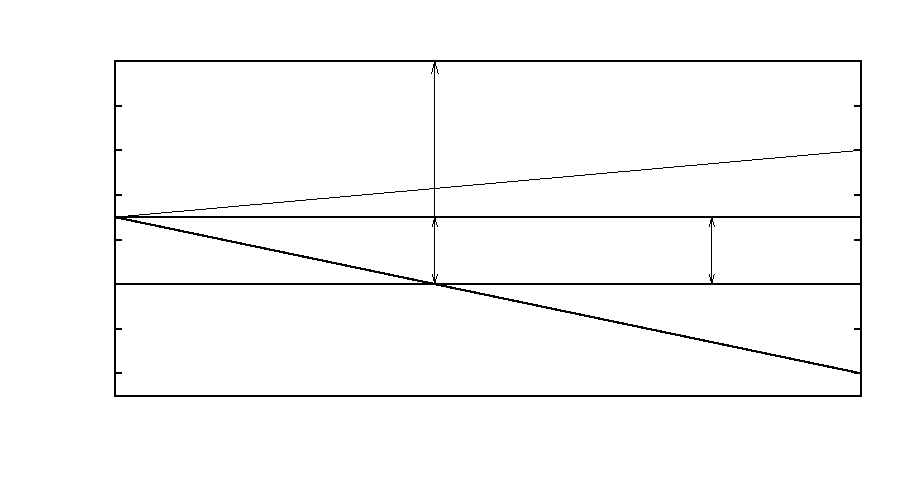
\includegraphics{conclusion}}%
    \gplfronttext
  \end{picture}%
\endgroup

		\caption{Components of the Vertical Velocity}
	\end{figure} 
%
In the deterministic module, ($v_{z,IMP,0}$) is calculated based on the four deterministic parameters.
$v_{z,IMP,0}$ is the estimated touchdown velocity that neglects the turbulences impact. In parallel, the turbulence intensity ($\sigma$) is estimated. It is an indication for the degree of trust that can be put into the deterministically calculated solution ($v_{z,IMP,0}$). In the Merge module of the algorithm, both branches are unified. This is done by estimating the probability that at the observed turbulence level, the variation $\Delta v_{z,IMP}$ caused by the turbulence is more than the tolerable variation $\Delta v_{z,crit}$. Through comparison of the computed probability and tolerable threshold it is decided whether a hard landing is predicted or not. An adaption of the threshold, enables the adjustment of the algorithm's sensitivity.\\
Regarding the proposed structure of the algorithm, the following benefits are obtained:\\
The uncertainty created by the random influence of the turbulence is rated through an observation of the turbulence level. In case of negligible turbulences, the calculation is reduced to a deterministic problem. An adaptive estimation is thus reached. In case of severe turbulences, where a purely deterministic prediction would fail the turbulence estimation provides an insight to the probability of a hard landing which is why the operating fiels of the algorithm is widened.
%
\newpage
\section{Deterministic Part}
To build a model, there are two opposed approaches.
%model building using explicit knowledge
\indent The first one is to build a model based on explicit knowledge. Within the multiple variants to express knowledge in a technical environment, physical statements are the most common in aerospace. This variant is reasonable, as long as the physics of the system are known or can be approximated without a significant lack in performance. The required offline processing power to build such a model is negligible, whereas the online processing power rises significantly with the model complexity. A simulator, for instance, that precisely computes the touchdown velocity $v_{z,IMP,0}$ based on a sophisticated physical model, requires much more processing power than available on board the aircraft. It is consequently challenging to find a model that is simple and at the same time performant.\\
Another option to build a model based on explicit knowledge is the fuzzy inference system. The knowledge is stored in the fuzzy rules and shapes of the membership functions (see Chapter 2). The design of a model based on fuzzy theory is reasonable, when intuitive - not physical - expert knowledge is available. It is human knowledge, stored in intuitively comprehensive if/then rules. Contrary to a model based on physics, a FIS requires only low online processing power - even when dealing with more complex systems. Nevertheless, finding adequate parameters of the Fuzzy system is often time-consuming and therefore less viable.\\
Both explicit methods, the one based on physics and the one based on if/then rules lead to "transparent" models, i.e models enabling to follow how the output of the system has been computed. In safety critical target environments like aerospace, this transparency of the model is a mandatory criterion for certification.\\
%model building using implicite knowledge
\indent The second approach is to build a model implicitly. In this context, neural networks have gained importance in the last decades. The basic idea is to derive a model by means of the knowledge that is hidden in matching input/output data pairs. In contrast to an explicitly built model, a large set of simulated or experimented I/O data is the driving source. Explicit knowledge is consequently no longer necessary, since the tuning of the parameters is done automatically. Compared to the options presented before, intellectual human capacity is saved during the design process. Nevertheless, the multiple simulations that have to be done in order to generate data pairs, demand enormous offline processing power.\\
Furthermore, a neural network can be regarded as a "black box", since it is hard to follow the contribution of a neuron to the final output \citet{Mackall2002}. Only neural networks containing a small number of neurons are rudimentary traceable. That is why neural networks are rarely implemented in aerospace systems. A method to avoid this disadvantage is the use of \gls{HIS}. The \gls{ANFIS} algorithm presented in (Chapter 2) unifies the advantages of both methods: learning from a data set, tracebility and low online processing power.\\
%
Relying on this argumentation, two algorithms that calculate the touchdown velocity ($v_{z,IMP,0}$) are proposed. The first one is an explicit model using the flight mechanical equations that are discussed in the theoretical foundations (analytical method). The second one is a Fuzzy Inference System built using the algorithm \gls{ANFIS} (Fuzzy ANFIS method).
%
\subsection{Analytical method}
According to the driven analysis of the automatic flare, the analytical formula is an attempt to unify all detected influences in one easily implementable mathematical expression, so that performant predictions can be reached.\\
The basic idea is to consider each part's contribution in one term and to unify all terms by summation.\\
The profile of the vertical velocity during the automatic flare, is given in equation 2.11. Integrating the flare duration (see equation 2.1) in the vertical velocity formula, one can compute the first basic term leading to $v_{z,IMP}(\gamma_{FIP,V_{gnd}})$:
%
			\begin{equation} 
				\begin{aligned}[H]
				v_{z}(t_{flare})=v_{z,IMP}=\, &a\,( \frac{1}{5}t_{flare}^5 - \tau t_{flare}^4 + 4\tau ^2 t_{flare}^3-12\tau ^3 																	t_{flare}^2+24\tau ^5-24\tau^5 e^\frac{-t_{flare}}{\tau})\\
								+\, &b\,( \frac{1}{4}t_{flare}^4 - \tau t_{flare}^3 + 3\tau ^2 t_{flare}^2 - 6 \tau ^3t_{flare}  + 6 																	\tau^4  + 6 \tau^4  e^\frac{-t_{flare}}{\tau} )\\
								+\, &c\,( \frac{1}{3}t_{flare}^3 - \tau t^2 + 2\tau ^2t_{flare}-2 \tau^3 +\tau^3 	e^\frac{-t_{flare}}{\tau})\\
								+\, &d\,(            t_{flare}   - \tau     +  \tau e^ \frac{-t_{flare}}{\tau})\\
								+\, &v_{z,FIP}\\
			\end{aligned}
	\end{equation}
%
where the sink rate at FIP is:
%
	\begin{equation}
		v_{z,FIP}=V_{gnd} \cdot tan(\gamma_{FIP})
	\end{equation}
%
The parameters (a,...,d) are interpolated based on the ground velocity at the moment the \gls{A/C} passes the FIP. 
It is pessimistically assumed, that the flare controller does not consider the runway slope, so that an additional term is evoked.
%
	\begin{equation}
		v_{z,IMP}(\gamma_{rwy})=V_{gnd}\cdot arctan(\gamma_{rwy})
	\end{equation}
%
The summation of both terms leads to $v_{z,IMP}(V_{gnd},\gamma_{FIP},\gamma_{rwy})$:
%
\begin{equation} 
				\begin{aligned}[H]
				v_{z,IMP}=\, &a\,( \frac{1}{5}t_{flare}^5 - \tau t_{flare}^4 + 4\tau ^2 	t_{flare}^3-12\tau ^3 t_{flare}^2+24\tau ^5-24\tau^5 e^\frac{-t_{flare}}{\tau})\\
								+\, &b\,( \frac{1}{4}t_{flare}^4 - \tau t_{flare}^3 + 3\tau ^2 t_{flare}^2 - 6 \tau ^3t_{flare}  + 6 																	\tau^4  + 6 \tau^4  e^\frac{-t_{flare}}{\tau} )\\
								+\, &c\,( \frac{1}{3}t_{flare}^3 - \tau t^2 + 2\tau ^2t_{flare}-2\tau^3+\tau^3 	e^\frac{-t_{flare}}{\tau})\\
								+\, &d\,(            t_{flare}   - \tau     +  \tau e^ \frac{-t_{flare}}{\tau})\\
								+\, &v_{z,FIP}\\
								+\, &V_{gnd}\cdot arctan(\gamma_{rwy})
			\end{aligned}
	\end{equation}
%
To consider load factors unequal to 1 ($\Delta n_{z,FIP}=1-n_{z,FIP}$) at FIP, following simplification is regarded:\\
as mentioned before \gls{A/C} and \gls{AP} are assumed to be a system of first order with a typical time constant of $\tau=1.5\,sec$. The transfer function of the \gls{A/C} is given with:
%
	\begin{equation}
  F=ke^{\frac{-t}{\tau}}
	\end{equation}
%
which is why:
%
	\begin{equation}
  	\Delta n_{z}(t)=1-n_{z,FIP}\cdot e{\frac{-t}{\tau}}.
	\end{equation}
%
Assuming that the flare control law does not consider the disturbance, an additional vertical velocity during the flare, caused by a load factor unequal to one, is:
%
	\begin{equation}
  	\Delta v_{z}(t)=g\cdot(1-n_{z,FIP}) \int_{0}^{t}e^{\frac{-\Delta T}{\tau} d}t = g\cdot(1-n_{z,FIP})\tau \left[-e^{\frac{-\Delta T}{\tau}}+1\right]
	\end{equation}
%
Inserting the known flare duration, one obtains:
%
	\begin{equation}
		\Delta v_{z,IMP}(\Delta n_{z,FIP})=\int_{0}^{t_flare} \Delta n_{z}e^{-\frac{t_flare}{\tau}}dt=\Delta n_{z}\tau 			\left[-e^{\frac{-\Delta t}{\tau}}+1\right]
	\end{equation}
%
A summation of all considered terms finally leads to an analytical calculation of the touchdown velocity, based on the four detected deterministic parameters:
\begin{equation} 
				\begin{aligned}[H]
				v_{z,IMP}= \, &a\,( \frac{1}{5}t_{flare}^5 - \tau t_{flare}^4 + 4\tau ^2 	t_{flare}^3-12\tau ^3 t_{flare}^2+24\tau 													^5-24\tau^5 e^\frac{-t_{flare}}{\tau})\\
								+\, &b\,( \frac{1}{4}t_{flare}^4 - \tau t_{flare}^3 + 3\tau ^2 t_{flare}^2 - 6 \tau ^3t_{flare}  + 6 																	\tau^4  + 6 \tau^4  e^\frac{-t_{flare}}{\tau} )\\
								+\, &c\,( \frac{1}{3}t_{flare}^3 - \tau t^2 + 2\tau ^2t_{flare}-2\tau^3+\tau^3 	e^\frac{-t_{flare}}{\tau})\\
								+\, &d\,(            t_{flare}   - \tau     +  \tau e^ \frac{-t_{flare}}{\tau})\\
								+\, &v_{z,FIP}\\
								+\, &V_{gnd}\cdot arctan(\gamma_{rwy})\\
								+\, &\Delta n_{z,FIP}\tau \left[-e^{\frac{-\Delta t}{\tau}}+1\right]\\
			\end{aligned}
	\end{equation}
%
\subsection{Fuzzy ANFIS method}
The core of the automatically constructed FIS is a set of representative related input/output data pairs:
%
	\begin{equation}
		\begin{bmatrix}
		\gamma_{FIP~1}&\gamma_{rwy~1}&V_{gnd~1}&n_{z,FIP~1}\\ \gamma_{FIP~2}&\gamma_{rwy~2}&V_{gnd~2}&n_{z,FIP~2}\\
		\quad\vdots & \quad\vdots & \quad\vdots & \quad\vdots\\ \gamma_{FIP~n}&\gamma_{rwy~n}&V_{gnd~n}&n_{z,FIP~n}\\
		\end{bmatrix}
		\Rightarrow
		\begin{bmatrix}
		v_{z,IMP,0~1}\\v_{z,IMP,0~2}\\\vdots\\v_{z,IMP,0~n}
		\end{bmatrix} 
	\end{equation}
%
\indent It is important to create various parameter constellations in order to store as much information as possible in the set. This is done by applying a sweep consisting of (n) simulations. In the employed sweep, the four parameters randomly vary within predefined margins. All remaining parameters that can be defined within the simulation are set to default values:
%
	\begin{equation}
		T=12.5^{\circ}\,C,\,Z_{rwy}=0\,m,\,c_{g}=38\%,\,m=390.000\,kg,\text{ landing configuration = full}
	\end{equation}
%
To define realistic margins, the following reasoning is used:\\
The operating field for the initial flight path angle ($\gamma_{FIP}$) is derived from a simple flight mechanical consideration since the \gls{A/C} configuration, mass ($m$) and thrust ($T$) affect the smallest possible ($\gamma_{FIP}$):\\
assuming that the thrust acts in the longitudinal axis of the \gls{A/C}, one can deduct the flight path angle out of the equilibrium of the forces in $x$-and $y$ direction as:
%
	\begin{equation}\left.\begin{aligned}
		\sum&=0=\frac{\rho}{2}\cdot V^2\cdot S \cdot c_D+mg~sin(\gamma)-T\\
		\sum&=0=\frac{\rho}{2}\cdot V^2\cdot S \cdot c_L-mg~cos(\gamma)
	\end{aligned}\right\}tan(\gamma)=\frac{T}{mg}-\frac{c_w}{c_a}\end{equation}
%
For Airbus aircraft, a glide ratio ($\frac{c_a}{c_w}$) of 10 can be assumed during landings. The steepest fpa is hence reached under idle:
%
	\begin{equation}
		\gamma_{min}=arctan(0-\frac{1}{10})=-5,71^{\,\circ} \sim-6^{\,\circ}
	\end{equation}
%
Assuming a maximum thrust-to-weight ratio of 0.6, equation 3.12 leads to an upper ($\gamma_{FIP}$) margin of $-2.2$�.\\
A typical operating field for the approach velocity of an Airbus aircraft is between 110 kt and 190 kt.\\
%
The operating area of the runway slope is derived from the certification specification for automatic landing performance:
%
	\begin{equation}
		-0.8\,\%<\gamma_{rwy}<+0.8\,\%
	\end{equation}
%
It is finally assumed that a reasonable load factor field at the entry of flare is:
%
	\begin{equation}
		+0.8\,g<n_{z,FIP}<+1.4\,g
	\end{equation}
%
Summing up, the following fields of operation are given:
%
	\begin{equation}
		\begin{aligned}
			-0.8\,\%&<&\gamma_{rwy}&<&+0.8\,\%\\
			-6^{\,\circ}&<&\gamma_{fip}&<&-2.2^{\,\circ}\\
			110\,kt&<&v_{wlong}&<&+190\,kt\\
			0.8\,g&<&n_{z,FIP}&<&+1.4\,g
		\end{aligned}
	\end{equation}
%
Generally, there are three parameters of freedom which can be adjusted when building an \gls{ANFIS}.\\
\indent The first parameter is the number of membership functions related to the inputs. This value is a compromise between performance and system complexity, since it dramatically increases the number of rules.\\
\indent The second parameter is the shape of the membership functions. The shapes can generally differ and exhibit any thinkable form within a FIS. However in this case one basic shape is globally employed, since the offline computational effort to build the \gls{ANFIS} raises significantly when relating individual shapes to each membership function. On top of this, a differentiable membership function is used because during the training mode, the least-squares algorithm applies a differentiation (see equation 3.27). Existing literature gives no heuristic about the use of certain shapes in dedicated situations. Contrary to a FIS that is explicitly built upon human expert knowledge, there is no rational argumentation in the choice of the membership function (in an \gls{ANFIS}).\\
\indent The last free parameter is the number of training epochs. Referring to \citet{Jang1996} and \citet{Negnevitsky2005} one can assume the performance of the FIS after the first training epoch to be a representative value of the reachable performance using the chosen configuration of parameters. Literature cites that the finding of the system with the highest performance is an iterative process. In consequence, the free parameters have to be varied until a satisfying performance is reached.\\
This method is applied to find a powerful $v_{z,IMP,0}$ estimation. The best result after one training epoch has been obtained using bell-shaped membership functions. The proposed FIS has a total number of 84 membership functions and 21 rules.
%
\subsection{Filtering Pilot Induced Loads}
Both presented deterministic estimators consider the load factor as an input parameter in their calculation. Since the aircraft's load at FIP is influenced by both, pilot induced loads and loads caused by the dynamic atmosphere, but only the first one has a stationary (deterministic) influence on the touchdown velocity, it is necessary to filter the dynamic atmosphere's loads. Therefore, a low  filter is employed to isolate the pilot induced loads. According to \citet{Rustenberg} the response of the aircraft's load caused by pilot stick inputs is not above 2Hz. That is why the cut off frequency of the low pass filter is set to this value.
%
\newpage
%
\section{Stochastical Part}
In order to estimate the level of vertical turbulences during the approach, the absolute value of the vertical wind has to be observed. Signals thus have to be used that fulfill both requirements: providing information about the vertical wind and being a measured value on board the \gls{A/C}. In this context, the angle of attack ($\alpha$) is an informative value, since it is directly dependent on the inflow i.e. on the wind direction. A change in the angle of attack, caused by the wind, impacts the flight path angle $\gamma$:
%
	\begin{equation}
		\gamma=\Theta-\alpha
	\end{equation}
%
and thus also the aerodynamic vertical load factor
%	
	\begin{equation}
		n_{z,fi}=\frac{V}{g}\dot{\gamma}+\cos\gamma=\frac{V}{g}\frac{\delta}{\delta(\Theta-\alpha)}+\cos(\Theta-\alpha)
	\end{equation}
%

$n_{z,fi}$ is a fictitious load factor assuming a massless aircraft. It provides information about load factor changes due both to variations in the vertical wind velocity and to \gls{A/C} responses induced through pilot commands. The true load factor $(n_{z,tr})$ measured on board the aircraft is due to the low pass characteristic of the true aircraft which is an aircraft with a mass unequal to zero much less affected by the change of the wind velocity.\\  
Assuming small flight path angles during the approach, one can facilitate the equation to:
%
	\begin{equation}
		n_{z,fi}=\frac{V}{g}(\dot{\Theta-\alpha})+1
	\end{equation}
%
The difference between the fictitious and the true load factor eliminates the influence of pilot induced loads.
%
	\begin{equation}
		 n_{z,tu}=n_{z,fi}-n_{z,tr}
	\end{equation}
%
where $(n_{z,tu})$ is considered as the wind load-factor. The integration of this value finally leads to the verticfial wind velocity:
%
	\begin{equation}
		g\cdot v_{w}=\int{n_{z,tu}}dt
	\end{equation}
%
%
	\begin{figure}[H]
			\flushleft
			\setlength\fboxsep{5pt}
			\fbox{\input{turbulence_estimator.pdf_tex}}  
			\caption{Block Diagram of the Vertical Wind  Estimator}
	\end{figure}
%
Inserting the vertical wind velocity in equation 2.17, the turbulence intensity is no longer an unknown value on board the aircraft:
%
	\begin{equation}
		\sigma=\sqrt{\frac{1}{t_o}\int_{0}^{t_{o}} v_{w}^2(t)dt}
	\end{equation}
%
\section{Merging both Branches}
The algorithm's merge part unifies both outputs, the deterministically calculated $v_{z,IMP,0}$ and the estimated tubulence intensity \textit{$\sigma_{est}$} so that a boolean can be set to \textit{true} in case of a predicted hard landing. 
%
\subsection{Probability Calculation}
%In order to find a relation between a given turbulence intensity and the variation it evokes on $v_{z,IMP,0}$ a statistical analysis is the only alternative, since one turbulence instensity level can result in multiple touchdown velocities as mentioned before.\\ To find this relation, simulation results of a reference approach:
%
%	\begin{center}
%		$\gamma_{FIP}=-3^{\,\circ},n_{z,FIP}=1,V_{gnd}=130\,kt,\gamma_{rwy}=0^{\,\circ}$
%	\end{center}
%
%are observed under three different turbulence levels:
%
%	\begin{compactitem}[$\bullet$]
%	  \setlength{\topsep}{3cm}
%			\item $\sigma_{1}$=1
%			\item $\sigma_{2}$=2.5
%			\item $\sigma_{3}$=5
%	\end{compactitem}
%
In order to find a relation between a given turbulence intensity and the variation it evokes on ($v_{z,IMP,0}$) a statistical analysis is the only alternative, since one turbulence instensity level can result in multiple touchdown velocities as mentioned before.
The "expectation" is introduced and defined as the sum of ($v_{z,IMP,0}$) and the mean deviation ($\mu_{\Delta v_{z,IMP}}$) a measured turbulence level evokes on it. ($\Delta v_{z,IMP,crit}$) is the buffer between the expectation and -10 [$\frac{ft}{sec}$]. It is consequently to compute the probability:
%
	\begin{equation}
		P(\Delta v_{z,IMP}=\Delta v_{z,IMP,crit})
	\end{equation}
%
\newpage
%
\noindent To find this relation, simulation results of a reference approach:
%
	\begin{center}
		$\gamma_{FIP}=-3^{\,\circ},n_{z,turb,FIP}=1,V_{gnd}=130\,kt,\gamma_{rwy}=0^{\,\circ}$
	\end{center}
%
are observed under three different turbulence levels:
%
	\begin{compactitem}[$\bullet$]
	  \setlength{\topsep}{3cm}
			\item $\sigma_{1}$=1
			\item $\sigma_{2}$=2.5
			\item $\sigma_{3}$=5
	\end{compactitem}
%
The resulting vertical touchdown velocity of the reference approach in case of no turbulences is -3 $[\frac{ft}{sec}]$. 
For each of the three turbulence levels the landing is repeated multiple times. By means of the resulting data pairs, three mean values for the vertical touchdown velocity ($\mu_{v_{z,IMP}}(\sigma_{1}),...,\mu_{v_{z,IMP}}(\sigma_{3})$) and the three variances ($V(\sigma_{1}),..., V(\sigma_{3})$) which are considered as supporting points are obtained (see Fig. 3.4).
The  mean deviation on the expectation which is to simplify assumed to be independent of $v_{z,IMP,0}$ is defined as:
%
	\begin{equation}
		\mu_{\Delta v_{z,IMP}}(\sigma)=\mu_{v_{z,IMP}}(\sigma)-3\,[\frac{ft}{sec}]
	\end{equation}
%
%The resulting vertical touchdown velocity of the reference approach in case of no turbulences is -3 $[\frac{ft}{sec}]$.\\
%To simplify, it is assumed that the statistical relation between a certain turbulence level and the mean deviation %($\mu_{\Delta v_{z,IMP}}$) it evokes around the expectation is not depending on $v_{z,IMP,0}$. The sum of $v_{z,IMP,0}$ and %the mean deviation is considered as expectation or static value. In the reference approach For each of the three turbulence %levels the landing is repeated multiple times. By means of the resulting data pairs, three mean values for the vertical %touchdown velocity ($\mu_{v_{z,IMP}}(\sigma_{1}),...,\mu_{v_{z,IMP}}(\sigma_{3})$) and the three variances %($V(\sigma_{1}),..., V(\sigma_{3})$) which are considered as supporting points are obtained (see Fig. 3.4). 
%
	\begin{figure}[H]
		% GNUPLOT: LaTeX picture with Postscript
\begingroup
  \makeatletter
  \providecommand\color[2][]{%
    \GenericError{(gnuplot) \space\space\space\@spaces}{%
      Package color not loaded in conjunction with
      terminal option `colourtext'%
    }{See the gnuplot documentation for explanation.%
    }{Either use 'blacktext' in gnuplot or load the package
      color.sty in LaTeX.}%
    \renewcommand\color[2][]{}%
  }%
  \providecommand\includegraphics[2][]{%
    \GenericError{(gnuplot) \space\space\space\@spaces}{%
      Package graphicx or graphics not loaded%
    }{See the gnuplot documentation for explanation.%
    }{The gnuplot epslatex terminal needs graphicx.sty or graphics.sty.}%
    \renewcommand\includegraphics[2][]{}%
  }%
  \providecommand\rotatebox[2]{#2}%
  \@ifundefined{ifGPcolor}{%
    \newif\ifGPcolor
    \GPcolorfalse
  }{}%
  \@ifundefined{ifGPblacktext}{%
    \newif\ifGPblacktext
    \GPblacktexttrue
  }{}%
  % define a \g@addto@macro without @ in the name:
  \let\gplgaddtomacro\g@addto@macro
  % define empty templates for all commands taking text:
  \gdef\gplbacktext{}%
  \gdef\gplfronttext{}%
  \makeatother
  \ifGPblacktext
    % no textcolor at all
    \def\colorrgb#1{}%
    \def\colorgray#1{}%
  \else
    % gray or color?
    \ifGPcolor
      \def\colorrgb#1{\color[rgb]{#1}}%
      \def\colorgray#1{\color[gray]{#1}}%
      \expandafter\def\csname LTw\endcsname{\color{white}}%
      \expandafter\def\csname LTb\endcsname{\color{black}}%
      \expandafter\def\csname LTa\endcsname{\color{black}}%
      \expandafter\def\csname LT0\endcsname{\color[rgb]{1,0,0}}%
      \expandafter\def\csname LT1\endcsname{\color[rgb]{0,1,0}}%
      \expandafter\def\csname LT2\endcsname{\color[rgb]{0,0,1}}%
      \expandafter\def\csname LT3\endcsname{\color[rgb]{1,0,1}}%
      \expandafter\def\csname LT4\endcsname{\color[rgb]{0,1,1}}%
      \expandafter\def\csname LT5\endcsname{\color[rgb]{1,1,0}}%
      \expandafter\def\csname LT6\endcsname{\color[rgb]{0,0,0}}%
      \expandafter\def\csname LT7\endcsname{\color[rgb]{1,0.3,0}}%
      \expandafter\def\csname LT8\endcsname{\color[rgb]{0.5,0.5,0.5}}%
    \else
      % gray
      \def\colorrgb#1{\color{black}}%
      \def\colorgray#1{\color[gray]{#1}}%
      \expandafter\def\csname LTw\endcsname{\color{white}}%
      \expandafter\def\csname LTb\endcsname{\color{black}}%
      \expandafter\def\csname LTa\endcsname{\color{black}}%
      \expandafter\def\csname LT0\endcsname{\color{black}}%
      \expandafter\def\csname LT1\endcsname{\color{black}}%
      \expandafter\def\csname LT2\endcsname{\color{black}}%
      \expandafter\def\csname LT3\endcsname{\color{black}}%
      \expandafter\def\csname LT4\endcsname{\color{black}}%
      \expandafter\def\csname LT5\endcsname{\color{black}}%
      \expandafter\def\csname LT6\endcsname{\color{black}}%
      \expandafter\def\csname LT7\endcsname{\color{black}}%
      \expandafter\def\csname LT8\endcsname{\color{black}}%
    \fi
  \fi
  \setlength{\unitlength}{0.0500bp}%
  \begin{picture}(9354.00,3230.00)%
    \gplgaddtomacro\gplbacktext{%
      \csname LTb\endcsname%
      \put(993,704){\makebox(0,0)[r]{\strut{} 0}}%
      \put(993,1332){\makebox(0,0)[r]{\strut{} 0.25}}%
      \put(993,1960){\makebox(0,0)[r]{\strut{} 0.5}}%
      \put(993,2588){\makebox(0,0)[r]{\strut{} 0.75}}%
      \put(1125,484){\makebox(0,0){\strut{}-6}}%
      \put(1778,484){\makebox(0,0){\strut{}-5.5}}%
      \put(2430,484){\makebox(0,0){\strut{}-5}}%
      \put(3083,484){\makebox(0,0){\strut{}-4.5}}%
      \put(3736,484){\makebox(0,0){\strut{}-4}}%
      \put(4388,484){\makebox(0,0){\strut{}-3.5}}%
      \put(5041,484){\makebox(0,0){\strut{}-3}}%
      \put(5694,484){\makebox(0,0){\strut{}-2.5}}%
      \put(6346,484){\makebox(0,0){\strut{}-2}}%
      \put(6999,484){\makebox(0,0){\strut{}-1.5}}%
      \put(7652,484){\makebox(0,0){\strut{}-1}}%
      \put(8304,484){\makebox(0,0){\strut{}-0.5}}%
      \put(8957,484){\makebox(0,0){\strut{} 0}}%
      \put(176,1834){\rotatebox{-270}{\makebox(0,0){\strut{}$\varphi(x)[-]$}}}%
      \put(5041,154){\makebox(0,0){\strut{}$v_{z,IMP}[\frac{ft}{sec}]$}}%
      \put(4858,2437){\makebox(0,0)[l]{\strut{}$V_{(\sigma_{i})}$}}%
      \put(4297,1307){\makebox(0,0)[l]{\strut{}$\rotatebox{90}{$\mu_{v_{z,IMP}}(\sigma_{i})$}$}}%
    }%
    \gplgaddtomacro\gplfronttext{%
    }%
    \gplbacktext
    \put(0,0){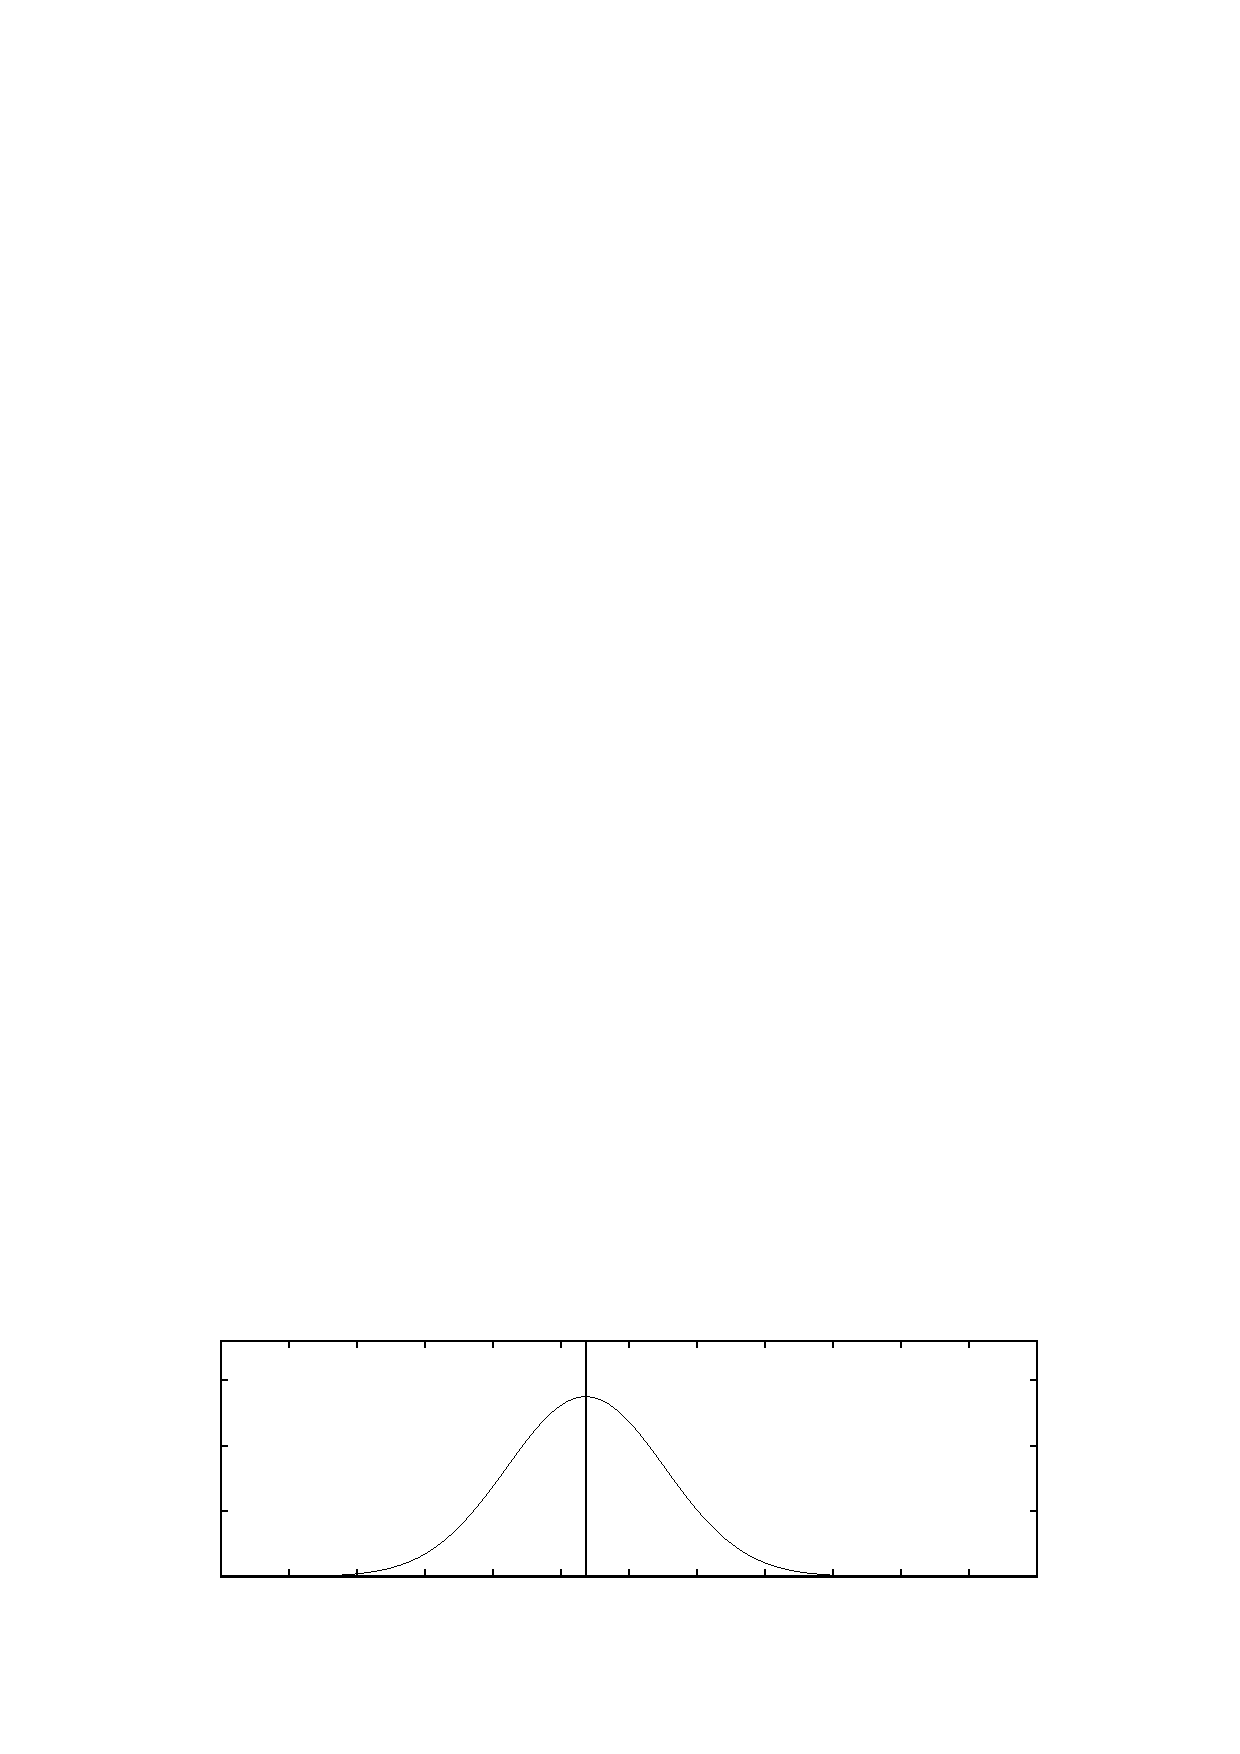
\includegraphics{bell_function_1}}%
    \gplfronttext
  \end{picture}%
\endgroup

		\caption{Normal Distribution of one Supporting Point}
	\end{figure}
	
%
The turbulence intensity observed during the approach ($\sigma_{est}$) is used to interpolate between the supporting points, so that ($\mu_{v_{z,IMP}}(\sigma_{est})$) i.e the mean vertical impact velocity  and the corresponding $V(\sigma_{est})$  variance of the vertical impact velocity ($V(\sigma_{est})$) can be computed under the observed turbulence intensity.
%
	\begin{figure}[H]                                   
		\begin{center}
			\setlength\fboxsep{5pt}
			\fbox{\begin{minipage}[t]{0.96\textwidth}
					\begingroup
						%LaTeX with PSTricks extensions
%%Creator: 0.48.2
%%Please note this file requires PSTricks extensions
\psset{xunit=.5pt,yunit=.5pt,runit=.5pt}
\begin{pspicture}(177.16534424,201.96850586)
{
\newrgbcolor{curcolor}{0 0 0}
\pscustom[linestyle=none,fillstyle=solid,fillcolor=curcolor,opacity=0.0056369]
{
\newpath
\moveto(32.63196945,172.48996521)
\lineto(126.89907455,172.48996521)
\lineto(126.89907455,129.3281038)
\lineto(32.63196945,129.3281038)
\closepath
}
}
{
\newrgbcolor{curcolor}{0 0 0}
\pscustom[linewidth=0.5669291,linecolor=curcolor]
{
\newpath
\moveto(32.63196945,172.48996521)
\lineto(126.89907455,172.48996521)
\lineto(126.89907455,129.3281038)
\lineto(32.63196945,129.3281038)
\closepath
}
}
{
\newrgbcolor{curcolor}{0 0 0}
\pscustom[linewidth=0.5669291,linecolor=curcolor]
{
\newpath
\moveto(-11.94482,150.61345586)
\lineto(30.415002,150.48414586)
}
}
{
\newrgbcolor{curcolor}{0 0 0}
\pscustom[linestyle=none,fillstyle=solid,fillcolor=curcolor]
{
\newpath
\moveto(28.14729616,150.49106839)
\lineto(27.00998197,149.36067673)
\lineto(30.98192846,150.48241523)
\lineto(27.0169045,151.62838257)
\lineto(28.14729616,150.49106839)
\closepath
}
}
{
\newrgbcolor{curcolor}{0 0 0}
\pscustom[linewidth=0.28346455,linecolor=curcolor]
{
\newpath
\moveto(28.14729616,150.49106839)
\lineto(27.00998197,149.36067673)
\lineto(30.98192846,150.48241523)
\lineto(27.0169045,151.62838257)
\lineto(28.14729616,150.49106839)
\closepath
}
}
{
\newrgbcolor{curcolor}{0 0 0}
\pscustom[linewidth=0.5669291,linecolor=curcolor]
{
\newpath
\moveto(126.79974,136.81662586)
\lineto(169.15956,136.68731586)
}
}
{
\newrgbcolor{curcolor}{0 0 0}
\pscustom[linestyle=none,fillstyle=solid,fillcolor=curcolor]
{
\newpath
\moveto(166.89185416,136.69423839)
\lineto(165.75453997,135.56384673)
\lineto(169.72648646,136.68558523)
\lineto(165.7614625,137.83155257)
\lineto(166.89185416,136.69423839)
\closepath
}
}
{
\newrgbcolor{curcolor}{0 0 0}
\pscustom[linewidth=0.28346455,linecolor=curcolor]
{
\newpath
\moveto(166.89185416,136.69423839)
\lineto(165.75453997,135.56384673)
\lineto(169.72648646,136.68558523)
\lineto(165.7614625,137.83155257)
\lineto(166.89185416,136.69423839)
\closepath
}
}
{
\newrgbcolor{curcolor}{0 0 0}
\pscustom[linewidth=0.5669291,linecolor=curcolor]
{
\newpath
\moveto(126.97199,156.51723586)
\lineto(171.6236,156.45133586)
}
}
{
\newrgbcolor{curcolor}{0 0 0}
\pscustom[linestyle=none,fillstyle=solid,fillcolor=curcolor]
{
\newpath
\moveto(169.35588606,156.45468271)
\lineto(168.22035567,155.32249917)
\lineto(172.19052848,156.45049915)
\lineto(168.22370252,157.59021311)
\lineto(169.35588606,156.45468271)
\closepath
}
}
{
\newrgbcolor{curcolor}{0 0 0}
\pscustom[linewidth=0.28346455,linecolor=curcolor]
{
\newpath
\moveto(169.35588606,156.45468271)
\lineto(168.22035567,155.32249917)
\lineto(172.19052848,156.45049915)
\lineto(168.22370252,157.59021311)
\lineto(169.35588606,156.45468271)
\closepath
}
}
{
\newrgbcolor{curcolor}{0 0 0}
\pscustom[linestyle=none,fillstyle=solid,fillcolor=curcolor]
{
\newpath
\moveto(165.96711731,145.69888855)
\lineto(162.91633606,153.57291199)
\lineto(164.04426575,153.57291199)
\lineto(166.09065247,147.85269715)
\curveto(166.25536262,147.39436212)(166.39322056,146.96467505)(166.50422668,146.56363465)
\curveto(166.62596772,146.99332085)(166.76740638,147.42300792)(166.92854309,147.85269715)
\lineto(169.05549622,153.57291199)
\lineto(170.11897278,153.57291199)
\lineto(167.03596497,145.69888855)
\closepath
}
}
{
\newrgbcolor{curcolor}{0 0 0}
\pscustom[linestyle=none,fillstyle=solid,fillcolor=curcolor]
{
\newpath
\moveto(172.78840637,143.38394715)
\curveto(172.25487569,144.05712587)(171.80370426,144.8448855)(171.43489075,145.7472284)
\curveto(171.06607479,146.6495712)(170.88166742,147.58414058)(170.88166809,148.55093934)
\curveto(170.88166742,149.40314917)(171.01952536,150.21955461)(171.29524231,151.00015809)
\curveto(171.61750653,151.90607636)(172.11522739,152.80841921)(172.78840637,153.70718934)
\lineto(173.48127747,153.70718934)
\curveto(173.0480064,152.96239041)(172.76154836,152.43065266)(172.62190247,152.11197449)
\curveto(172.4034758,151.61782795)(172.23160097,151.10220346)(172.10627747,150.56509949)
\curveto(171.95230438,149.89549894)(171.87531877,149.22232253)(171.87532043,148.54556824)
\curveto(171.87531877,146.82323639)(172.41063725,145.10269774)(173.48127747,143.38394715)
\closepath
}
}
{
\newrgbcolor{curcolor}{0 0 0}
\pscustom[linestyle=none,fillstyle=solid,fillcolor=curcolor]
{
\newpath
\moveto(176.6287384,144.56558777)
\lineto(176.6287384,145.53238465)
\curveto(176.14533771,145.59325715)(175.75235308,145.7015741)(175.44978333,145.85733582)
\curveto(175.14721045,146.01309722)(174.88581749,146.2646432)(174.66560364,146.61197449)
\curveto(174.44538824,146.95930396)(174.3173773,147.38361994)(174.28157043,147.88492371)
\lineto(175.2537384,148.0675409)
\curveto(175.32893228,147.54833332)(175.46141912,147.16698604)(175.65119934,146.92349793)
\curveto(175.92333272,146.57974705)(176.24917875,146.38817823)(176.6287384,146.3487909)
\lineto(176.6287384,149.42642762)
\curveto(176.23127512,149.50161913)(175.82486277,149.65559033)(175.40950012,149.88834168)
\curveto(175.1015562,150.06021232)(174.86433313,150.29833057)(174.6978302,150.60269715)
\curveto(174.53132565,150.90705392)(174.44807378,151.25259394)(174.44807434,151.63931824)
\curveto(174.44807378,152.32681161)(174.69156312,152.88361444)(175.17854309,153.3097284)
\curveto(175.50438783,153.59617883)(175.98778578,153.77163439)(176.6287384,153.83609559)
\lineto(176.6287384,154.29800965)
\lineto(177.19807434,154.29800965)
\lineto(177.19807434,153.83609559)
\curveto(177.76024495,153.78237656)(178.20604528,153.61766319)(178.53547668,153.34195496)
\curveto(178.95799766,152.99103621)(179.21222917,152.50942862)(179.298172,151.89713074)
\lineto(178.29914856,151.74674012)
\curveto(178.24185254,152.12629098)(178.12279341,152.41722494)(177.94197083,152.61954285)
\curveto(177.76114013,152.82184693)(177.51317488,152.95522895)(177.19807434,153.01968934)
\lineto(177.19807434,150.23209168)
\curveto(177.68504971,150.11034248)(178.00731501,150.01545325)(178.16487122,149.94742371)
\curveto(178.46564789,149.81493262)(178.71092759,149.65379996)(178.90071106,149.46402527)
\curveto(179.0904845,149.27424305)(179.23639907,149.04865734)(179.3384552,148.78726746)
\curveto(179.44050043,148.5258714)(179.49152577,148.24299408)(179.49153137,147.93863465)
\curveto(179.49152577,147.26903672)(179.2784726,146.71044353)(178.85237122,146.2628534)
\curveto(178.42625991,145.81526214)(177.87482817,145.57535352)(177.19807434,145.54312684)
\lineto(177.19807434,144.56558777)
\closepath
\moveto(176.6287384,153.03043152)
\curveto(176.25275948,152.97313258)(175.95645444,152.82274211)(175.73982239,152.57925965)
\curveto(175.52318664,152.33576343)(175.41486969,152.04751502)(175.41487122,151.71451355)
\curveto(175.41486969,151.38508079)(175.50707337,151.10936492)(175.69148254,150.88736512)
\curveto(175.87588811,150.66535494)(176.18830642,150.48810903)(176.6287384,150.35562684)
\closepath
\moveto(177.19807434,146.3487909)
\curveto(177.57404722,146.39533968)(177.88467516,146.5582627)(178.12995911,146.83756043)
\curveto(178.37523457,147.11685589)(178.49787442,147.46239591)(178.49787903,147.87418152)
\curveto(178.49787442,148.22509046)(178.41104182,148.5070726)(178.23738098,148.72012879)
\curveto(178.06371144,148.93317894)(177.71727624,149.12385258)(177.19807434,149.29215027)
\closepath
}
}
{
\newrgbcolor{curcolor}{0 0 0}
\pscustom[linestyle=none,fillstyle=solid,fillcolor=curcolor]
{
\newpath
\moveto(182.29524231,145.56461121)
\lineto(180.01252747,153.70718934)
\lineto(180.79133606,153.70718934)
\lineto(183.06867981,145.56461121)
\closepath
}
}
{
\newrgbcolor{curcolor}{0 0 0}
\pscustom[linestyle=none,fillstyle=solid,fillcolor=curcolor]
{
\newpath
\moveto(183.40168762,147.40152527)
\lineto(184.35774231,147.5519159)
\curveto(184.4114519,147.16877641)(184.56094719,146.87515691)(184.80622864,146.67105652)
\curveto(185.0515066,146.46695419)(185.39436107,146.36490351)(185.83479309,146.36490418)
\curveto(186.27880029,146.36490351)(186.60822705,146.45531683)(186.82307434,146.63614441)
\curveto(187.03791412,146.81697012)(187.14533588,147.02912811)(187.14533997,147.27261902)
\curveto(187.14533588,147.49104171)(187.05044666,147.66291654)(186.860672,147.78824402)
\curveto(186.72818135,147.87417935)(186.3987546,147.98339148)(185.87239075,148.11588074)
\curveto(185.16340427,148.2949146)(184.67194969,148.44978099)(184.39802551,148.58048035)
\curveto(184.12409867,148.71117395)(183.91641659,148.8920006)(183.77497864,149.12296082)
\curveto(183.63353927,149.3539142)(183.56281994,149.60904089)(183.56282043,149.88834168)
\curveto(183.56281994,150.14256901)(183.62100673,150.37800171)(183.73738098,150.59464051)
\curveto(183.85375389,150.81126951)(184.012201,150.99120097)(184.21272278,151.13443543)
\curveto(184.3631121,151.24543249)(184.56810864,151.33942653)(184.82771301,151.41641785)
\curveto(185.08731385,151.49339773)(185.36571527,151.53189053)(185.66291809,151.53189637)
\curveto(186.11050619,151.53189053)(186.50349082,151.46743747)(186.84187317,151.33853699)
\curveto(187.18024796,151.20962523)(187.43000357,151.03506486)(187.59114075,150.81485535)
\curveto(187.75226887,150.59463561)(187.86327136,150.30012093)(187.92414856,149.93131043)
\lineto(186.97883606,149.80240418)
\curveto(186.93586344,150.09601957)(186.81143322,150.32518601)(186.60554504,150.48990418)
\curveto(186.39964978,150.65461277)(186.10871583,150.73696945)(185.73274231,150.73697449)
\curveto(185.28872967,150.73696945)(184.97183545,150.66356458)(184.78205872,150.51675965)
\curveto(184.59227854,150.36994508)(184.49738931,150.19807025)(184.49739075,150.00113465)
\curveto(184.49738931,149.87580495)(184.53677729,149.76301209)(184.61555481,149.66275574)
\curveto(184.69432922,149.55891074)(184.81786425,149.47297332)(184.98616028,149.40494324)
\curveto(185.08283795,149.36913228)(185.36750563,149.28677559)(185.84016418,149.15787293)
\curveto(186.52407999,148.97525247)(187.00121168,148.82575717)(187.27156067,148.7093866)
\curveto(187.54190124,148.59301001)(187.75405923,148.42382073)(187.90803528,148.20181824)
\curveto(188.06200163,147.97981075)(188.13898723,147.70409488)(188.13899231,147.3746698)
\curveto(188.13898723,147.05240283)(188.04499319,146.74893633)(187.85700989,146.46426941)
\curveto(187.669017,146.17960096)(187.39777704,145.95938634)(187.04328918,145.80362488)
\curveto(186.68879337,145.64786322)(186.28775211,145.56998243)(185.84016418,145.5699823)
\curveto(185.09895121,145.56998243)(184.53409175,145.72395363)(184.14558411,146.03189637)
\curveto(183.7570743,146.33983843)(183.50910905,146.79638095)(183.40168762,147.40152527)
\closepath
}
}
{
\newrgbcolor{curcolor}{0 0 0}
\pscustom[linestyle=none,fillstyle=solid,fillcolor=curcolor]
{
\newpath
\moveto(189.29377747,152.46109559)
\lineto(189.29377747,153.57291199)
\lineto(190.26057434,153.57291199)
\lineto(190.26057434,152.46109559)
\closepath
\moveto(189.29377747,145.69888855)
\lineto(189.29377747,151.40299012)
\lineto(190.26057434,151.40299012)
\lineto(190.26057434,145.69888855)
\closepath
}
}
{
\newrgbcolor{curcolor}{0 0 0}
\pscustom[linestyle=none,fillstyle=solid,fillcolor=curcolor]
{
\newpath
\moveto(191.56037903,145.2262323)
\lineto(192.50032043,145.08658387)
\curveto(192.53970693,144.79654571)(192.64891906,144.5852829)(192.82795715,144.4527948)
\curveto(193.06786395,144.27375977)(193.39550034,144.18424163)(193.81086731,144.18424012)
\curveto(194.25845521,144.18424163)(194.60399523,144.27375977)(194.8474884,144.4527948)
\curveto(195.09097391,144.63183233)(195.25568729,144.88248312)(195.34162903,145.20474793)
\curveto(195.39175486,145.40168833)(195.41502957,145.81526214)(195.41145325,146.44547059)
\curveto(194.98892323,145.94774898)(194.46255657,145.69888855)(193.83235168,145.69888855)
\curveto(193.04816996,145.69888855)(192.44123697,145.98176588)(192.0115509,146.54752137)
\curveto(191.58186283,147.11327516)(191.3670193,147.79182266)(191.36701965,148.5831659)
\curveto(191.3670193,149.1274333)(191.46548925,149.62963007)(191.66242981,150.0897577)
\curveto(191.85936907,150.54987654)(192.14493193,150.90526356)(192.51911926,151.1559198)
\curveto(192.89330358,151.40656514)(193.33283765,151.53189053)(193.83772278,151.53189637)
\curveto(194.51089636,151.53189053)(195.06590883,151.25975539)(195.50276184,150.71549012)
\lineto(195.50276184,151.40299012)
\lineto(196.3943634,151.40299012)
\lineto(196.3943634,146.47232605)
\curveto(196.39435802,145.58430534)(196.3039447,144.95499281)(196.12312317,144.5843866)
\curveto(195.94229142,144.21378262)(195.65583337,143.9210583)(195.26374817,143.70621277)
\curveto(194.87165447,143.49137123)(194.38915169,143.38394946)(193.8162384,143.38394715)
\curveto(193.13589774,143.38394946)(192.58625636,143.53702548)(192.16731262,143.84317566)
\curveto(191.74836657,144.14932956)(191.54605558,144.61034798)(191.56037903,145.2262323)
\closepath
\moveto(192.360672,148.65299012)
\curveto(192.36067065,147.90461552)(192.50927076,147.35855486)(192.80647278,147.01480652)
\curveto(193.10367121,146.67105555)(193.47606667,146.49918072)(193.92366028,146.49918152)
\curveto(194.36766734,146.49918072)(194.7400628,146.67016037)(195.04084778,147.01212098)
\curveto(195.3416247,147.35407896)(195.49201517,147.89029261)(195.49201965,148.62076355)
\curveto(195.49201517,149.31900212)(195.33714879,149.84536878)(195.02742004,150.19986512)
\curveto(194.71768327,150.55435245)(194.34439262,150.73159837)(193.907547,150.7316034)
\curveto(193.47785703,150.73159837)(193.11262302,150.55703799)(192.81184387,150.20792176)
\curveto(192.51106112,149.8587965)(192.36067065,149.34048648)(192.360672,148.65299012)
\closepath
}
}
{
\newrgbcolor{curcolor}{0 0 0}
\pscustom[linestyle=none,fillstyle=solid,fillcolor=curcolor]
{
\newpath
\moveto(197.860672,145.69888855)
\lineto(197.860672,151.40299012)
\lineto(198.72541809,151.40299012)
\lineto(198.72541809,150.60269715)
\curveto(198.90445278,150.88198884)(199.14257103,151.10667937)(199.43977356,151.27676941)
\curveto(199.73697148,151.4468483)(200.07535005,151.53189053)(200.45491028,151.53189637)
\curveto(200.87743258,151.53189053)(201.22386778,151.44416276)(201.49421692,151.26871277)
\curveto(201.76455734,151.09325165)(201.95523098,150.84797195)(202.0662384,150.53287293)
\curveto(202.5174049,151.19888305)(203.10464389,151.53189053)(203.82795715,151.53189637)
\curveto(204.3937051,151.53189053)(204.82876326,151.37523379)(205.13313293,151.06192566)
\curveto(205.43748661,150.74860681)(205.58966745,150.26610404)(205.5896759,149.6144159)
\lineto(205.5896759,145.69888855)
\lineto(204.62825012,145.69888855)
\lineto(204.62825012,149.29215027)
\curveto(204.62824263,149.67886504)(204.59691128,149.95726646)(204.53425598,150.12735535)
\curveto(204.47158589,150.29743539)(204.35789785,150.43439814)(204.19319153,150.53824402)
\curveto(204.02847109,150.64208023)(203.83511191,150.69400075)(203.6131134,150.69400574)
\curveto(203.21206566,150.69400075)(202.87905818,150.56061872)(202.61408997,150.29385926)
\curveto(202.34911079,150.02709061)(202.21662395,149.60008908)(202.21662903,149.0128534)
\lineto(202.21662903,145.69888855)
\lineto(201.24983215,145.69888855)
\lineto(201.24983215,149.40494324)
\curveto(201.24982804,149.83462661)(201.17105208,150.15689191)(201.01350403,150.37174012)
\curveto(200.85594822,150.58657898)(200.59813598,150.69400075)(200.24006653,150.69400574)
\curveto(199.96792828,150.69400075)(199.71638231,150.62238624)(199.48542786,150.47916199)
\curveto(199.25446871,150.33592819)(199.08706979,150.12645574)(198.98323059,149.85074402)
\curveto(198.8793877,149.575024)(198.82746718,149.17756346)(198.82746887,148.65836121)
\lineto(198.82746887,145.69888855)
\closepath
}
}
{
\newrgbcolor{curcolor}{0 0 0}
\pscustom[linestyle=none,fillstyle=solid,fillcolor=curcolor]
{
\newpath
\moveto(210.75666809,146.40250184)
\curveto(210.39859108,146.09813946)(210.05394625,145.88329592)(209.72273254,145.75797059)
\curveto(209.39151201,145.63264513)(209.036125,145.56998243)(208.65657043,145.5699823)
\curveto(208.02994111,145.56998243)(207.54833352,145.72305845)(207.21174622,146.02921082)
\curveto(206.87515711,146.33536253)(206.70686301,146.7265568)(206.7068634,147.2027948)
\curveto(206.70686301,147.4820899)(206.77042089,147.73721659)(206.89753723,147.96817566)
\curveto(207.0246524,148.1991302)(207.19115614,148.38443274)(207.39704895,148.52408387)
\curveto(207.60293958,148.66372934)(207.83479157,148.76936074)(208.09260559,148.8409784)
\curveto(208.28238226,148.89110541)(208.56884031,148.93944521)(208.95198059,148.98599793)
\curveto(209.73257613,149.07909351)(210.30728258,149.190096)(210.67610168,149.31900574)
\curveto(210.67967804,149.45148897)(210.68146841,149.53563602)(210.68147278,149.57144715)
\curveto(210.68146841,149.96532309)(210.5901599,150.24282932)(210.407547,150.40396668)
\curveto(210.16047283,150.62238624)(209.79344846,150.73159837)(209.30647278,150.7316034)
\curveto(208.85171763,150.73159837)(208.51602461,150.65192722)(208.2993927,150.49258973)
\curveto(208.08275681,150.33324264)(207.92251934,150.0512605)(207.81867981,149.64664246)
\lineto(206.87336731,149.77554871)
\curveto(206.95930416,150.18016663)(207.10074282,150.50690784)(207.29768372,150.75577332)
\curveto(207.49462263,151.00462869)(207.77929032,151.19619751)(208.15168762,151.33048035)
\curveto(208.52408124,151.46475193)(208.95555867,151.53189053)(209.44612122,151.53189637)
\curveto(209.93309676,151.53189053)(210.32876694,151.47459892)(210.63313293,151.36002137)
\curveto(210.93749029,151.24543249)(211.16128563,151.10130828)(211.30451965,150.92764832)
\curveto(211.44774368,150.7539779)(211.548004,150.53465846)(211.6053009,150.26968934)
\curveto(211.63752214,150.10497139)(211.6536354,149.80777116)(211.65364075,149.37808777)
\lineto(211.65364075,148.08902527)
\curveto(211.6536354,147.19026076)(211.67422457,146.62182057)(211.71540833,146.38370301)
\curveto(211.75658126,146.14558407)(211.83804277,145.91731282)(211.95979309,145.69888855)
\lineto(210.95002747,145.69888855)
\curveto(210.84976251,145.89940919)(210.78530945,146.13394671)(210.75666809,146.40250184)
\closepath
\moveto(210.67610168,148.56168152)
\curveto(210.32518621,148.41844964)(209.79881955,148.29670497)(209.09700012,148.19644715)
\curveto(208.69953679,148.13915304)(208.41844984,148.07469998)(208.2537384,148.00308777)
\curveto(208.08902308,147.93147096)(207.96190732,147.82673473)(207.87239075,147.68887879)
\curveto(207.78287104,147.55101886)(207.73811197,147.39794285)(207.7381134,147.22965027)
\curveto(207.73811197,146.9718365)(207.83568675,146.75699297)(208.03083801,146.58511902)
\curveto(208.22598584,146.41324331)(208.5115487,146.3273059)(208.88752747,146.32730652)
\curveto(209.25992035,146.3273059)(209.59113747,146.4087674)(209.88117981,146.57169129)
\curveto(210.17121501,146.73461343)(210.38426818,146.9575136)(210.52033997,147.24039246)
\curveto(210.6241768,147.45881518)(210.67609732,147.78108048)(210.67610168,148.20718934)
\closepath
}
}
{
\newrgbcolor{curcolor}{0 0 0}
\pscustom[linestyle=none,fillstyle=solid,fillcolor=curcolor]
{
\newpath
\moveto(212.26594543,143.5128534)
\lineto(212.26594543,144.21109559)
\lineto(218.67366028,144.21109559)
\lineto(218.67366028,143.5128534)
\closepath
}
}
{
\newrgbcolor{curcolor}{0 0 0}
\pscustom[linestyle=none,fillstyle=solid,fillcolor=curcolor]
{
\newpath
\moveto(218.86164856,148.98599793)
\curveto(219.13736412,148.99315609)(219.36205465,149.06745615)(219.53572083,149.20889832)
\curveto(219.70938504,149.35033347)(219.82486344,149.54458783)(219.88215637,149.79166199)
\curveto(219.93944665,150.03872796)(219.96988282,150.46125358)(219.97346497,151.05924012)
\curveto(219.97704427,151.65721593)(219.98778645,152.05109574)(220.00569153,152.24088074)
\curveto(220.03791661,152.54165515)(220.09789376,152.78335413)(220.18562317,152.9659784)
\curveto(220.27334932,153.14858814)(220.38166626,153.2945027)(220.51057434,153.40372254)
\curveto(220.63947851,153.51292696)(220.80419188,153.59617883)(221.00471497,153.6534784)
\curveto(221.14078009,153.6892777)(221.36278508,153.70718133)(221.67073059,153.70718934)
\lineto(221.97151184,153.70718934)
\lineto(221.97151184,152.86392762)
\lineto(221.80500793,152.86392762)
\curveto(221.43260922,152.86392045)(221.18553916,152.79678185)(221.063797,152.6625116)
\curveto(220.94204982,152.52822743)(220.88117748,152.22834166)(220.88117981,151.7628534)
\curveto(220.88117748,150.82469723)(220.86148349,150.23208715)(220.82209778,149.98502137)
\curveto(220.75764245,149.60187944)(220.64753514,149.30646958)(220.49177551,149.0987909)
\curveto(220.33601201,148.89110541)(220.09162749,148.70669805)(219.75862122,148.54556824)
\curveto(220.15249983,148.38085202)(220.43806269,148.12930605)(220.61531067,147.79092957)
\curveto(220.79255453,147.45254891)(220.88117748,146.89843163)(220.88117981,146.12857605)
\curveto(220.88117748,145.43033414)(220.88833894,145.01496997)(220.90266418,144.8824823)
\curveto(220.93130764,144.63899378)(221.00381734,144.46890932)(221.12019348,144.3722284)
\curveto(221.2365645,144.27555013)(221.46483575,144.22721034)(221.80500793,144.22720887)
\lineto(221.97151184,144.22720887)
\lineto(221.97151184,143.38394715)
\lineto(221.67073059,143.38394715)
\curveto(221.31981637,143.38394946)(221.06558485,143.41259527)(220.90803528,143.46988465)
\curveto(220.67886649,143.55224357)(220.48908803,143.68562559)(220.33869934,143.87003113)
\curveto(220.18830708,144.05444033)(220.09073231,144.28808267)(220.04597473,144.57095887)
\curveto(220.00121417,144.85383732)(219.97704427,145.31754128)(219.97346497,145.96207215)
\curveto(219.96988282,146.60660249)(219.93944665,147.05240283)(219.88215637,147.29947449)
\curveto(219.82486344,147.54654296)(219.70938504,147.7416925)(219.53572083,147.88492371)
\curveto(219.36205465,148.02815055)(219.13736412,148.10334579)(218.86164856,148.11050965)
\closepath
}
}
{
\newrgbcolor{curcolor}{0 0 0}
\pscustom[linestyle=none,fillstyle=solid,fillcolor=curcolor]
{
\newpath
\moveto(226.85920715,147.53580262)
\lineto(227.85823059,147.41226746)
\curveto(227.70067304,146.82860748)(227.4088439,146.37564569)(226.98274231,146.05338074)
\curveto(226.55663121,145.73111508)(226.01236092,145.56998243)(225.34992981,145.5699823)
\curveto(224.51561763,145.56998243)(223.85407858,145.82689949)(223.36531067,146.34073426)
\curveto(222.87654049,146.85456774)(222.63215597,147.57518876)(222.63215637,148.50259949)
\curveto(222.63215597,149.46223115)(222.87922603,150.20702207)(223.37336731,150.73697449)
\curveto(223.8675063,151.26691684)(224.50845618,151.53189053)(225.29621887,151.53189637)
\curveto(226.05891035,151.53189053)(226.68195661,151.27228793)(227.1653595,150.75308777)
\curveto(227.64875252,150.23387751)(227.89045149,149.50340949)(227.89045715,148.56168152)
\curveto(227.89045149,148.50438705)(227.88866113,148.41844964)(227.88508606,148.30386902)
\lineto(223.63117981,148.30386902)
\curveto(223.66698566,147.67723944)(223.84423158,147.19742221)(224.16291809,146.8644159)
\curveto(224.48160073,146.53140725)(224.87906127,146.36490351)(225.3553009,146.36490418)
\curveto(225.70978961,146.36490351)(226.01236092,146.45800238)(226.26301575,146.64420105)
\curveto(226.5136625,146.83039784)(226.71239277,147.12759806)(226.85920715,147.53580262)
\closepath
\moveto(223.68489075,149.0987909)
\lineto(226.86994934,149.0987909)
\curveto(226.82697599,149.57860473)(226.70523132,149.93846765)(226.50471497,150.17838074)
\curveto(226.19676829,150.55077172)(225.79751739,150.73696945)(225.30696106,150.73697449)
\curveto(224.86294801,150.73696945)(224.48965737,150.58836934)(224.18708801,150.29117371)
\curveto(223.88451474,149.9939689)(223.71711582,149.59650835)(223.68489075,149.0987909)
\closepath
}
}
{
\newrgbcolor{curcolor}{0 0 0}
\pscustom[linestyle=none,fillstyle=solid,fillcolor=curcolor]
{
\newpath
\moveto(228.69075012,147.40152527)
\lineto(229.64680481,147.5519159)
\curveto(229.7005144,147.16877641)(229.85000969,146.87515691)(230.09529114,146.67105652)
\curveto(230.3405691,146.46695419)(230.68342357,146.36490351)(231.12385559,146.36490418)
\curveto(231.56786279,146.36490351)(231.89728955,146.45531683)(232.11213684,146.63614441)
\curveto(232.32697662,146.81697012)(232.43439838,147.02912811)(232.43440247,147.27261902)
\curveto(232.43439838,147.49104171)(232.33950916,147.66291654)(232.1497345,147.78824402)
\curveto(232.01724385,147.87417935)(231.6878171,147.98339148)(231.16145325,148.11588074)
\curveto(230.45246677,148.2949146)(229.96101219,148.44978099)(229.68708801,148.58048035)
\curveto(229.41316117,148.71117395)(229.20547909,148.8920006)(229.06404114,149.12296082)
\curveto(228.92260177,149.3539142)(228.85188244,149.60904089)(228.85188293,149.88834168)
\curveto(228.85188244,150.14256901)(228.91006923,150.37800171)(229.02644348,150.59464051)
\curveto(229.14281639,150.81126951)(229.3012635,150.99120097)(229.50178528,151.13443543)
\curveto(229.6521746,151.24543249)(229.85717114,151.33942653)(230.11677551,151.41641785)
\curveto(230.37637635,151.49339773)(230.65477777,151.53189053)(230.95198059,151.53189637)
\curveto(231.39956869,151.53189053)(231.79255332,151.46743747)(232.13093567,151.33853699)
\curveto(232.46931046,151.20962523)(232.71906607,151.03506486)(232.88020325,150.81485535)
\curveto(233.04133137,150.59463561)(233.15233386,150.30012093)(233.21321106,149.93131043)
\lineto(232.26789856,149.80240418)
\curveto(232.22492594,150.09601957)(232.10049572,150.32518601)(231.89460754,150.48990418)
\curveto(231.68871228,150.65461277)(231.39777833,150.73696945)(231.02180481,150.73697449)
\curveto(230.57779217,150.73696945)(230.26089795,150.66356458)(230.07112122,150.51675965)
\curveto(229.88134104,150.36994508)(229.78645181,150.19807025)(229.78645325,150.00113465)
\curveto(229.78645181,149.87580495)(229.82583979,149.76301209)(229.90461731,149.66275574)
\curveto(229.98339172,149.55891074)(230.10692675,149.47297332)(230.27522278,149.40494324)
\curveto(230.37190045,149.36913228)(230.65656813,149.28677559)(231.12922668,149.15787293)
\curveto(231.81314249,148.97525247)(232.29027418,148.82575717)(232.56062317,148.7093866)
\curveto(232.83096374,148.59301001)(233.04312173,148.42382073)(233.19709778,148.20181824)
\curveto(233.35106413,147.97981075)(233.42804973,147.70409488)(233.42805481,147.3746698)
\curveto(233.42804973,147.05240283)(233.33405569,146.74893633)(233.14607239,146.46426941)
\curveto(232.9580795,146.17960096)(232.68683954,145.95938634)(232.33235168,145.80362488)
\curveto(231.97785587,145.64786322)(231.57681461,145.56998243)(231.12922668,145.5699823)
\curveto(230.38801371,145.56998243)(229.82315425,145.72395363)(229.43464661,146.03189637)
\curveto(229.0461368,146.33983843)(228.79817155,146.79638095)(228.69075012,147.40152527)
\closepath
}
}
{
\newrgbcolor{curcolor}{0 0 0}
\pscustom[linestyle=none,fillstyle=solid,fillcolor=curcolor]
{
\newpath
\moveto(236.68830872,146.56363465)
\lineto(236.82795715,145.70963074)
\curveto(236.55581903,145.65233912)(236.31232969,145.62369332)(236.0974884,145.62369324)
\curveto(235.74657505,145.62369332)(235.47443991,145.67919456)(235.28108215,145.79019715)
\curveto(235.08772154,145.90119955)(234.95165397,146.04711412)(234.87287903,146.22794129)
\curveto(234.79410204,146.4087674)(234.75471406,146.7892195)(234.75471497,147.36929871)
\lineto(234.75471497,150.65103699)
\lineto(234.04573059,150.65103699)
\lineto(234.04573059,151.40299012)
\lineto(234.75471497,151.40299012)
\lineto(234.75471497,152.81558777)
\lineto(235.71614075,153.3956659)
\lineto(235.71614075,151.40299012)
\lineto(236.68830872,151.40299012)
\lineto(236.68830872,150.65103699)
\lineto(235.71614075,150.65103699)
\lineto(235.71614075,147.31558777)
\curveto(235.71613888,147.03987029)(235.73314733,146.86262437)(235.76716614,146.78384949)
\curveto(235.80118112,146.70507244)(235.85668236,146.64240975)(235.93367004,146.59586121)
\curveto(236.01065356,146.54931088)(236.12076087,146.52603617)(236.26399231,146.52603699)
\curveto(236.37141167,146.52603617)(236.51285033,146.5385687)(236.68830872,146.56363465)
\closepath
}
}
{
\newrgbcolor{curcolor}{0 0 0}
\pscustom[linestyle=none,fillstyle=solid,fillcolor=curcolor]
{
\newpath
\moveto(240.26545715,148.98599793)
\lineto(240.26545715,148.11050965)
\curveto(239.98973792,148.10334579)(239.76504739,148.02815055)(239.59138489,147.88492371)
\curveto(239.41771701,147.7416925)(239.30223861,147.54743814)(239.24494934,147.30216004)
\curveto(239.18765539,147.05687873)(239.15721922,146.6352483)(239.15364075,146.03726746)
\curveto(239.15005777,145.43928595)(239.13931559,145.04540614)(239.12141418,144.85562684)
\curveto(239.08918544,144.551266)(239.02920828,144.30867185)(238.94148254,144.12784363)
\curveto(238.85375273,143.94701856)(238.74543578,143.80199918)(238.61653137,143.69278504)
\curveto(238.48762354,143.58357491)(238.32291016,143.50032304)(238.12239075,143.44302918)
\curveto(237.98632196,143.40364345)(237.76431697,143.38394946)(237.45637512,143.38394715)
\lineto(237.15559387,143.38394715)
\lineto(237.15559387,144.22720887)
\lineto(237.32209778,144.22720887)
\curveto(237.69449282,144.22721034)(237.94156289,144.29434894)(238.06330872,144.42862488)
\curveto(238.18505223,144.56290336)(238.24592456,144.86457949)(238.2459259,145.33365418)
\curveto(238.24592456,146.22883594)(238.26203783,146.79638095)(238.29426575,147.0362909)
\curveto(238.35155597,147.4337501)(238.46613918,147.7515395)(238.63801575,147.98966004)
\curveto(238.80988884,148.227776)(239.05337818,148.41307855)(239.3684845,148.54556824)
\curveto(238.95669859,148.7425053)(238.66665982,149.00300309)(238.49836731,149.32706238)
\curveto(238.33007161,149.65111442)(238.24592456,150.19807025)(238.2459259,150.96793152)
\curveto(238.24592456,151.66616774)(238.23697275,152.08332227)(238.21907043,152.21939637)
\curveto(238.19400404,152.45929846)(238.12328471,152.62669738)(238.00691223,152.72159363)
\curveto(237.89053755,152.81647584)(237.66226629,152.86392045)(237.32209778,152.86392762)
\lineto(237.15559387,152.86392762)
\lineto(237.15559387,153.70718934)
\lineto(237.45637512,153.70718934)
\curveto(237.80728568,153.70718133)(238.06151719,153.67853552)(238.21907043,153.62125184)
\curveto(238.44823556,153.54246795)(238.63801401,153.4099811)(238.78840637,153.2237909)
\curveto(238.93879496,153.03758564)(239.03636973,152.80304812)(239.08113098,152.52017762)
\curveto(239.12588787,152.23729347)(239.15005777,151.77358951)(239.15364075,151.12906434)
\curveto(239.15721922,150.4845283)(239.18765539,150.03962315)(239.24494934,149.79434754)
\curveto(239.30223861,149.54906374)(239.41771701,149.35480938)(239.59138489,149.21158387)
\curveto(239.76504739,149.06835133)(239.98973792,148.99315609)(240.26545715,148.98599793)
\closepath
}
}
{
\newrgbcolor{curcolor}{0 0 0}
\pscustom[linestyle=none,fillstyle=solid,fillcolor=curcolor]
{
\newpath
\moveto(243.3162384,144.56558777)
\lineto(243.3162384,145.53238465)
\curveto(242.83283771,145.59325715)(242.43985308,145.7015741)(242.13728333,145.85733582)
\curveto(241.83471045,146.01309722)(241.57331749,146.2646432)(241.35310364,146.61197449)
\curveto(241.13288824,146.95930396)(241.0048773,147.38361994)(240.96907043,147.88492371)
\lineto(241.9412384,148.0675409)
\curveto(242.01643228,147.54833332)(242.14891912,147.16698604)(242.33869934,146.92349793)
\curveto(242.61083272,146.57974705)(242.93667875,146.38817823)(243.3162384,146.3487909)
\lineto(243.3162384,149.42642762)
\curveto(242.91877512,149.50161913)(242.51236277,149.65559033)(242.09700012,149.88834168)
\curveto(241.7890562,150.06021232)(241.55183313,150.29833057)(241.3853302,150.60269715)
\curveto(241.21882565,150.90705392)(241.13557378,151.25259394)(241.13557434,151.63931824)
\curveto(241.13557378,152.32681161)(241.37906312,152.88361444)(241.86604309,153.3097284)
\curveto(242.19188783,153.59617883)(242.67528578,153.77163439)(243.3162384,153.83609559)
\lineto(243.3162384,154.29800965)
\lineto(243.88557434,154.29800965)
\lineto(243.88557434,153.83609559)
\curveto(244.44774495,153.78237656)(244.89354528,153.61766319)(245.22297668,153.34195496)
\curveto(245.64549766,152.99103621)(245.89972917,152.50942862)(245.985672,151.89713074)
\lineto(244.98664856,151.74674012)
\curveto(244.92935254,152.12629098)(244.81029341,152.41722494)(244.62947083,152.61954285)
\curveto(244.44864013,152.82184693)(244.20067488,152.95522895)(243.88557434,153.01968934)
\lineto(243.88557434,150.23209168)
\curveto(244.37254971,150.11034248)(244.69481501,150.01545325)(244.85237122,149.94742371)
\curveto(245.15314789,149.81493262)(245.39842759,149.65379996)(245.58821106,149.46402527)
\curveto(245.7779845,149.27424305)(245.92389907,149.04865734)(246.0259552,148.78726746)
\curveto(246.12800043,148.5258714)(246.17902577,148.24299408)(246.17903137,147.93863465)
\curveto(246.17902577,147.26903672)(245.9659726,146.71044353)(245.53987122,146.2628534)
\curveto(245.11375991,145.81526214)(244.56232817,145.57535352)(243.88557434,145.54312684)
\lineto(243.88557434,144.56558777)
\closepath
\moveto(243.3162384,153.03043152)
\curveto(242.94025948,152.97313258)(242.64395444,152.82274211)(242.42732239,152.57925965)
\curveto(242.21068664,152.33576343)(242.10236969,152.04751502)(242.10237122,151.71451355)
\curveto(242.10236969,151.38508079)(242.19457337,151.10936492)(242.37898254,150.88736512)
\curveto(242.56338811,150.66535494)(242.87580642,150.48810903)(243.3162384,150.35562684)
\closepath
\moveto(243.88557434,146.3487909)
\curveto(244.26154722,146.39533968)(244.57217516,146.5582627)(244.81745911,146.83756043)
\curveto(245.06273457,147.11685589)(245.18537442,147.46239591)(245.18537903,147.87418152)
\curveto(245.18537442,148.22509046)(245.09854182,148.5070726)(244.92488098,148.72012879)
\curveto(244.75121144,148.93317894)(244.40477624,149.12385258)(243.88557434,149.29215027)
\closepath
}
}
{
\newrgbcolor{curcolor}{0 0 0}
\pscustom[linestyle=none,fillstyle=solid,fillcolor=curcolor]
{
\newpath
\moveto(248.05891418,143.38394715)
\lineto(247.36604309,143.38394715)
\curveto(248.43667938,145.10269774)(248.97199785,146.82323639)(248.97200012,148.54556824)
\curveto(248.97199785,149.21874181)(248.89501225,149.88654713)(248.74104309,150.54898621)
\curveto(248.61929638,151.0860902)(248.44921191,151.60171468)(248.23078918,152.09586121)
\curveto(248.09113936,152.41812012)(247.80289095,152.95522895)(247.36604309,153.70718934)
\lineto(248.05891418,153.70718934)
\curveto(248.73208924,152.80841921)(249.22981009,151.90607636)(249.55207825,151.00015809)
\curveto(249.82779127,150.21955461)(249.9656492,149.40314917)(249.96565247,148.55093934)
\curveto(249.9656492,147.58414058)(249.78034665,146.6495712)(249.40974426,145.7472284)
\curveto(249.03913645,144.8448855)(248.58886021,144.05712587)(248.05891418,143.38394715)
\closepath
}
}
{
\newrgbcolor{curcolor}{0 0 0}
\pscustom[linestyle=none,fillstyle=solid,fillcolor=curcolor]
{
\newpath
\moveto(169.10725403,162.77988221)
\lineto(169.10725403,163.74667908)
\curveto(168.62385333,163.80755158)(168.2308687,163.91586853)(167.92829895,164.07163025)
\curveto(167.62572608,164.22739166)(167.36433311,164.47893763)(167.14411926,164.82626893)
\curveto(166.92390386,165.17359839)(166.79589292,165.59791438)(166.76008606,166.09921814)
\lineto(167.73225403,166.28183533)
\curveto(167.8074479,165.76262775)(167.93993475,165.38128048)(168.12971497,165.13779236)
\curveto(168.40184835,164.79404148)(168.72769438,164.60247266)(169.10725403,164.56308533)
\lineto(169.10725403,167.64072205)
\curveto(168.70979075,167.71591356)(168.3033784,167.86988476)(167.88801575,168.10263611)
\curveto(167.58007183,168.27450675)(167.34284876,168.512625)(167.17634583,168.81699158)
\curveto(167.00984128,169.12134835)(166.92658941,169.46688837)(166.92658997,169.85361268)
\curveto(166.92658941,170.54110605)(167.17007875,171.09790888)(167.65705872,171.52402283)
\curveto(167.98290346,171.81047327)(168.46630141,171.98592882)(169.10725403,172.05039002)
\lineto(169.10725403,172.51230408)
\lineto(169.67658997,172.51230408)
\lineto(169.67658997,172.05039002)
\curveto(170.23876057,171.996671)(170.68456091,171.83195762)(171.01399231,171.55624939)
\curveto(171.43651328,171.20533064)(171.6907448,170.72372305)(171.77668762,170.11142518)
\lineto(170.77766418,169.96103455)
\curveto(170.72036817,170.34058542)(170.60130904,170.63151937)(170.42048645,170.83383729)
\curveto(170.23965576,171.03614136)(169.99169051,171.16952339)(169.67658997,171.23398377)
\lineto(169.67658997,168.44638611)
\curveto(170.16356534,168.32463691)(170.48583064,168.22974768)(170.64338684,168.16171814)
\curveto(170.94416351,168.02922705)(171.18944322,167.8680944)(171.37922668,167.67831971)
\curveto(171.56900013,167.48853749)(171.7149147,167.26295177)(171.81697083,167.00156189)
\curveto(171.91901606,166.74016584)(171.9700414,166.45728852)(171.970047,166.15292908)
\curveto(171.9700414,165.48333116)(171.75698822,164.92473797)(171.33088684,164.47714783)
\curveto(170.90477553,164.02955657)(170.35334379,163.78964796)(169.67658997,163.75742127)
\lineto(169.67658997,162.77988221)
\closepath
\moveto(169.10725403,171.24472596)
\curveto(168.7312751,171.18742702)(168.43497006,171.03703654)(168.21833801,170.79355408)
\curveto(168.00170226,170.55005786)(167.89338532,170.26180945)(167.89338684,169.92880799)
\curveto(167.89338532,169.59937522)(167.985589,169.32365935)(168.16999817,169.10165955)
\curveto(168.35440373,168.87964938)(168.66682204,168.70240346)(169.10725403,168.56992127)
\closepath
\moveto(169.67658997,164.56308533)
\curveto(170.05256284,164.60963411)(170.36319079,164.77255713)(170.60847473,165.05185486)
\curveto(170.85375019,165.33115032)(170.97639004,165.67669034)(170.97639465,166.08847596)
\curveto(170.97639004,166.43938489)(170.88955745,166.72136703)(170.71589661,166.93442322)
\curveto(170.54222707,167.14747337)(170.19579187,167.33814701)(169.67658997,167.50644471)
\closepath
}
}
{
\newrgbcolor{curcolor}{0 0 0}
\pscustom[linestyle=none,fillstyle=solid,fillcolor=curcolor]
{
\newpath
\moveto(174.77375793,163.77890564)
\lineto(172.49104309,171.92148377)
\lineto(173.26985168,171.92148377)
\lineto(175.54719543,163.77890564)
\closepath
}
}
{
\newrgbcolor{curcolor}{0 0 0}
\pscustom[linestyle=none,fillstyle=solid,fillcolor=curcolor]
{
\newpath
\moveto(176.266922,163.91318299)
\lineto(176.266922,169.61728455)
\lineto(177.13166809,169.61728455)
\lineto(177.13166809,168.81699158)
\curveto(177.31070278,169.09628327)(177.54882103,169.3209738)(177.84602356,169.49106385)
\curveto(178.14322148,169.66114274)(178.48160005,169.74618497)(178.86116028,169.7461908)
\curveto(179.28368258,169.74618497)(179.63011778,169.65845719)(179.90046692,169.48300721)
\curveto(180.17080734,169.30754608)(180.36148098,169.06226638)(180.4724884,168.74716736)
\curveto(180.9236549,169.41317749)(181.51089389,169.74618497)(182.23420715,169.7461908)
\curveto(182.7999551,169.74618497)(183.23501326,169.58952822)(183.53938293,169.2762201)
\curveto(183.84373661,168.96290125)(183.99591745,168.48039847)(183.9959259,167.82871033)
\lineto(183.9959259,163.91318299)
\lineto(183.03450012,163.91318299)
\lineto(183.03450012,167.50644471)
\curveto(183.03449263,167.89315948)(183.00316128,168.17156089)(182.94050598,168.34164979)
\curveto(182.87783589,168.51172982)(182.76414785,168.64869258)(182.59944153,168.75253846)
\curveto(182.43472109,168.85637466)(182.24136191,168.90829518)(182.0193634,168.90830018)
\curveto(181.61831566,168.90829518)(181.28530818,168.77491315)(181.02033997,168.50815369)
\curveto(180.75536079,168.24138504)(180.62287395,167.81438351)(180.62287903,167.22714783)
\lineto(180.62287903,163.91318299)
\lineto(179.65608215,163.91318299)
\lineto(179.65608215,167.61923768)
\curveto(179.65607804,168.04892104)(179.57730208,168.37118634)(179.41975403,168.58603455)
\curveto(179.26219822,168.80087341)(179.00438598,168.90829518)(178.64631653,168.90830018)
\curveto(178.37417828,168.90829518)(178.12263231,168.83668067)(177.89167786,168.69345643)
\curveto(177.66071871,168.55022262)(177.49331979,168.34075018)(177.38948059,168.06503846)
\curveto(177.2856377,167.78931844)(177.23371718,167.3918579)(177.23371887,166.87265564)
\lineto(177.23371887,163.91318299)
\closepath
}
}
{
\newrgbcolor{curcolor}{0 0 0}
\pscustom[linestyle=none,fillstyle=solid,fillcolor=curcolor]
{
\newpath
\moveto(189.17903137,163.91318299)
\lineto(189.17903137,164.75107361)
\curveto(188.73501694,164.10654217)(188.13166467,163.78427687)(187.36897278,163.78427674)
\curveto(187.03238192,163.78427687)(186.71817325,163.84872993)(186.42634583,163.97763611)
\curveto(186.13451498,164.10654217)(185.91788108,164.26857)(185.77644348,164.4637201)
\curveto(185.63500376,164.65886909)(185.53563862,164.89788252)(185.47834778,165.18076111)
\curveto(185.43895903,165.3705383)(185.41926504,165.67131925)(185.41926575,166.08310486)
\lineto(185.41926575,169.61728455)
\lineto(186.38606262,169.61728455)
\lineto(186.38606262,166.45371033)
\curveto(186.38606095,165.94882548)(186.40575494,165.60865655)(186.44514465,165.43320252)
\curveto(186.50601526,165.17896948)(186.63492138,164.97934403)(186.8318634,164.83432557)
\curveto(187.02880119,164.68930526)(187.27229053,164.61679557)(187.56233215,164.61679627)
\curveto(187.85236808,164.61679557)(188.12450322,164.69109562)(188.3787384,164.83969666)
\curveto(188.63296626,164.98829585)(188.81289772,165.19060684)(188.91853333,165.44663025)
\curveto(189.02416053,165.7026506)(189.07697623,166.07415088)(189.07698059,166.56113221)
\lineto(189.07698059,169.61728455)
\lineto(190.04377747,169.61728455)
\lineto(190.04377747,163.91318299)
\closepath
}
}
{
\newrgbcolor{curcolor}{0 0 0}
\pscustom[linestyle=none,fillstyle=solid,fillcolor=curcolor]
{
\newpath
\moveto(190.67219543,161.72714783)
\lineto(190.67219543,162.42539002)
\lineto(197.07991028,162.42539002)
\lineto(197.07991028,161.72714783)
\closepath
}
}
{
\newrgbcolor{curcolor}{0 0 0}
\pscustom[linestyle=none,fillstyle=solid,fillcolor=curcolor]
{
\newpath
\moveto(197.26789856,167.20029236)
\curveto(197.54361412,167.20745053)(197.76830465,167.28175058)(197.94197083,167.42319275)
\curveto(198.11563504,167.5646279)(198.23111344,167.75888227)(198.28840637,168.00595643)
\curveto(198.34569665,168.2530224)(198.37613282,168.67554802)(198.37971497,169.27353455)
\curveto(198.38329427,169.87151036)(198.39403645,170.26539018)(198.41194153,170.45517518)
\curveto(198.44416661,170.75594958)(198.50414376,170.99764856)(198.59187317,171.18027283)
\curveto(198.67959932,171.36288257)(198.78791626,171.50879714)(198.91682434,171.61801697)
\curveto(199.04572851,171.7272214)(199.21044188,171.81047327)(199.41096497,171.86777283)
\curveto(199.54703009,171.90357213)(199.76903508,171.92147576)(200.07698059,171.92148377)
\lineto(200.37776184,171.92148377)
\lineto(200.37776184,171.07822205)
\lineto(200.21125793,171.07822205)
\curveto(199.83885922,171.07821489)(199.59178916,171.01107628)(199.470047,170.87680604)
\curveto(199.34829982,170.74252186)(199.28742748,170.44263609)(199.28742981,169.97714783)
\curveto(199.28742748,169.03899166)(199.26773349,168.44638158)(199.22834778,168.1993158)
\curveto(199.16389245,167.81617388)(199.05378514,167.52076402)(198.89802551,167.31308533)
\curveto(198.74226201,167.10539985)(198.49787749,166.92099248)(198.16487122,166.75986268)
\curveto(198.55874983,166.59514645)(198.84431269,166.34360048)(199.02156067,166.005224)
\curveto(199.19880453,165.66684334)(199.28742748,165.11272606)(199.28742981,164.34287049)
\curveto(199.28742748,163.64462857)(199.29458894,163.2292644)(199.30891418,163.09677674)
\curveto(199.33755764,162.85328821)(199.41006734,162.68320375)(199.52644348,162.58652283)
\curveto(199.6428145,162.48984457)(199.87108575,162.44150477)(200.21125793,162.4415033)
\lineto(200.37776184,162.4415033)
\lineto(200.37776184,161.59824158)
\lineto(200.07698059,161.59824158)
\curveto(199.72606637,161.5982439)(199.47183485,161.6268897)(199.31428528,161.68417908)
\curveto(199.08511649,161.766538)(198.89533803,161.89992003)(198.74494934,162.08432557)
\curveto(198.59455708,162.26873476)(198.49698231,162.50237711)(198.45222473,162.7852533)
\curveto(198.40746417,163.06813175)(198.38329427,163.53183571)(198.37971497,164.17636658)
\curveto(198.37613282,164.82089692)(198.34569665,165.26669726)(198.28840637,165.51376893)
\curveto(198.23111344,165.76083739)(198.11563504,165.95598694)(197.94197083,166.09921814)
\curveto(197.76830465,166.24244498)(197.54361412,166.31764022)(197.26789856,166.32480408)
\closepath
}
}
{
\newrgbcolor{curcolor}{0 0 0}
\pscustom[linestyle=none,fillstyle=solid,fillcolor=curcolor]
{
\newpath
\moveto(202.91828918,163.77890564)
\lineto(200.63557434,171.92148377)
\lineto(201.41438293,171.92148377)
\lineto(203.69172668,163.77890564)
\closepath
}
}
{
\newrgbcolor{curcolor}{0 0 0}
\pscustom[linestyle=none,fillstyle=solid,fillcolor=curcolor]
{
\newpath
\moveto(204.5349884,163.91318299)
\lineto(204.5349884,171.78720643)
\lineto(207.24739075,171.78720643)
\curveto(207.85969126,171.78719855)(208.32697595,171.74960093)(208.64924622,171.67441346)
\curveto(209.10041268,171.57056465)(209.48534068,171.38257656)(209.80403137,171.11044861)
\curveto(210.21938942,170.75953031)(210.53001737,170.31104443)(210.73591614,169.76498963)
\curveto(210.94180081,169.21892313)(211.04474667,168.59498169)(211.04475403,167.89316346)
\curveto(211.04474667,167.2951783)(210.97492252,166.76523092)(210.83528137,166.30331971)
\curveto(210.69562593,165.84140372)(210.51658965,165.45916126)(210.298172,165.15659119)
\curveto(210.07974112,164.85401864)(209.84072769,164.61590038)(209.58113098,164.44223572)
\curveto(209.32152248,164.26857)(209.00820899,164.13697834)(208.64118958,164.04746033)
\curveto(208.27416025,163.95794206)(207.85252981,163.91318299)(207.376297,163.91318299)
\closepath
\moveto(205.57698059,164.84238221)
\lineto(207.25813293,164.84238221)
\curveto(207.77733457,164.84238128)(208.18464211,164.89072107)(208.48005676,164.98740174)
\curveto(208.77546183,165.08408025)(209.01089454,165.22014783)(209.18635559,165.39560486)
\curveto(209.43342016,165.64267345)(209.62588416,165.97478574)(209.76374817,166.39194275)
\curveto(209.90160003,166.80909481)(209.97052899,167.31487229)(209.97053528,167.90927674)
\curveto(209.97052899,168.73283963)(209.8353566,169.36573287)(209.5650177,169.80795838)
\curveto(209.29466704,170.25017209)(208.96613547,170.54647714)(208.579422,170.69687439)
\curveto(208.30012051,170.80428938)(207.85073945,170.85800026)(207.23127747,170.85800721)
\lineto(205.57698059,170.85800721)
\closepath
}
}
{
\newrgbcolor{curcolor}{0 0 0}
\pscustom[linestyle=none,fillstyle=solid,fillcolor=curcolor]
{
\newpath
\moveto(216.26545715,165.75009705)
\lineto(217.26448059,165.62656189)
\curveto(217.10692304,165.04290191)(216.8150939,164.58994012)(216.38899231,164.26767518)
\curveto(215.96288121,163.94540952)(215.41861092,163.78427687)(214.75617981,163.78427674)
\curveto(213.92186763,163.78427687)(213.26032858,164.04119393)(212.77156067,164.55502869)
\curveto(212.28279049,165.06886217)(212.03840597,165.7894832)(212.03840637,166.71689393)
\curveto(212.03840597,167.67652558)(212.28547603,168.4213165)(212.77961731,168.95126893)
\curveto(213.2737563,169.48121127)(213.91470618,169.74618497)(214.70246887,169.7461908)
\curveto(215.46516035,169.74618497)(216.08820661,169.48658236)(216.5716095,168.96738221)
\curveto(217.05500252,168.44817194)(217.29670149,167.71770392)(217.29670715,166.77597596)
\curveto(217.29670149,166.71868148)(217.29491113,166.63274407)(217.29133606,166.51816346)
\lineto(213.03742981,166.51816346)
\curveto(213.07323566,165.89153387)(213.25048158,165.41171665)(213.56916809,165.07871033)
\curveto(213.88785073,164.74570169)(214.28531127,164.57919795)(214.7615509,164.57919861)
\curveto(215.11603961,164.57919795)(215.41861092,164.67229681)(215.66926575,164.85849549)
\curveto(215.9199125,165.04469227)(216.11864277,165.3418925)(216.26545715,165.75009705)
\closepath
\moveto(213.09114075,167.31308533)
\lineto(216.27619934,167.31308533)
\curveto(216.23322599,167.79289916)(216.11148132,168.15276208)(215.91096497,168.39267518)
\curveto(215.60301829,168.76506616)(215.20376739,168.95126389)(214.71321106,168.95126893)
\curveto(214.26919801,168.95126389)(213.89590737,168.80266378)(213.59333801,168.50546814)
\curveto(213.29076474,168.20826333)(213.12336582,167.81080279)(213.09114075,167.31308533)
\closepath
}
}
{
\newrgbcolor{curcolor}{0 0 0}
\pscustom[linestyle=none,fillstyle=solid,fillcolor=curcolor]
{
\newpath
\moveto(218.4622345,163.91318299)
\lineto(218.4622345,171.78720643)
\lineto(219.42903137,171.78720643)
\lineto(219.42903137,163.91318299)
\closepath
}
}
{
\newrgbcolor{curcolor}{0 0 0}
\pscustom[linestyle=none,fillstyle=solid,fillcolor=curcolor]
{
\newpath
\moveto(223.04377747,164.77792908)
\lineto(223.1834259,163.92392518)
\curveto(222.91128778,163.86663356)(222.66779844,163.83798775)(222.45295715,163.83798768)
\curveto(222.1020438,163.83798775)(221.82990866,163.893489)(221.6365509,164.00449158)
\curveto(221.44319029,164.11549398)(221.30712272,164.26140855)(221.22834778,164.44223572)
\curveto(221.14957079,164.62306184)(221.11018281,165.00351393)(221.11018372,165.58359314)
\lineto(221.11018372,168.86533143)
\lineto(220.40119934,168.86533143)
\lineto(220.40119934,169.61728455)
\lineto(221.11018372,169.61728455)
\lineto(221.11018372,171.02988221)
\lineto(222.0716095,171.60996033)
\lineto(222.0716095,169.61728455)
\lineto(223.04377747,169.61728455)
\lineto(223.04377747,168.86533143)
\lineto(222.0716095,168.86533143)
\lineto(222.0716095,165.52988221)
\curveto(222.07160763,165.25416472)(222.08861608,165.0769188)(222.12263489,164.99814393)
\curveto(222.15664987,164.91936688)(222.21215111,164.85670418)(222.28913879,164.81015564)
\curveto(222.36612231,164.76360531)(222.47622962,164.7403306)(222.61946106,164.74033143)
\curveto(222.72688042,164.7403306)(222.86831908,164.75286314)(223.04377747,164.77792908)
\closepath
}
}
{
\newrgbcolor{curcolor}{0 0 0}
\pscustom[linestyle=none,fillstyle=solid,fillcolor=curcolor]
{
\newpath
\moveto(227.70588684,164.61679627)
\curveto(227.34780983,164.31243389)(227.003165,164.09759036)(226.67195129,163.97226502)
\curveto(226.34073076,163.84693956)(225.98534375,163.78427687)(225.60578918,163.78427674)
\curveto(224.97915986,163.78427687)(224.49755227,163.93735289)(224.16096497,164.24350525)
\curveto(223.82437586,164.54965696)(223.65608176,164.94085123)(223.65608215,165.41708924)
\curveto(223.65608176,165.69638433)(223.71963964,165.95151103)(223.84675598,166.1824701)
\curveto(223.97387115,166.41342463)(224.14037489,166.59872718)(224.3462677,166.7383783)
\curveto(224.55215833,166.87802377)(224.78401032,166.98365518)(225.04182434,167.05527283)
\curveto(225.23160101,167.10539985)(225.51805906,167.15373964)(225.90119934,167.20029236)
\curveto(226.68179488,167.29338794)(227.25650133,167.40439043)(227.62532043,167.53330018)
\curveto(227.62889679,167.6657834)(227.63068716,167.74993045)(227.63069153,167.78574158)
\curveto(227.63068716,168.17961752)(227.53937865,168.45712376)(227.35676575,168.61826111)
\curveto(227.10969158,168.83668067)(226.74266721,168.9458928)(226.25569153,168.94589783)
\curveto(225.80093638,168.9458928)(225.46524336,168.86622166)(225.24861145,168.70688416)
\curveto(225.03197556,168.54753708)(224.87173809,168.26555494)(224.76789856,167.86093689)
\lineto(223.82258606,167.98984314)
\curveto(223.90852291,168.39446106)(224.04996157,168.72120227)(224.24690247,168.97006775)
\curveto(224.44384138,169.21892313)(224.72850907,169.41049194)(225.10090637,169.54477479)
\curveto(225.47329999,169.67904636)(225.90477742,169.74618497)(226.39533997,169.7461908)
\curveto(226.88231551,169.74618497)(227.27798569,169.68889336)(227.58235168,169.5743158)
\curveto(227.88670904,169.45972692)(228.11050438,169.31560272)(228.2537384,169.14194275)
\curveto(228.39696243,168.96827233)(228.49722275,168.74895289)(228.55451965,168.48398377)
\curveto(228.58674089,168.31926582)(228.60285415,168.0220656)(228.6028595,167.59238221)
\lineto(228.6028595,166.30331971)
\curveto(228.60285415,165.40455519)(228.62344332,164.83611501)(228.66462708,164.59799744)
\curveto(228.70580001,164.35987851)(228.78726152,164.13160725)(228.90901184,163.91318299)
\lineto(227.89924622,163.91318299)
\curveto(227.79898126,164.11370362)(227.7345282,164.34824115)(227.70588684,164.61679627)
\closepath
\moveto(227.62532043,166.77597596)
\curveto(227.27440496,166.63274407)(226.7480383,166.5109994)(226.04621887,166.41074158)
\curveto(225.64875554,166.35344748)(225.36766859,166.28899441)(225.20295715,166.21738221)
\curveto(225.03824183,166.14576539)(224.91112607,166.04102917)(224.8216095,165.90317322)
\curveto(224.73208979,165.7653133)(224.68733072,165.61223728)(224.68733215,165.44394471)
\curveto(224.68733072,165.18613093)(224.7849055,164.9712874)(224.98005676,164.79941346)
\curveto(225.17520459,164.62753774)(225.46076745,164.54160033)(225.83674622,164.54160096)
\curveto(226.2091391,164.54160033)(226.54035622,164.62306184)(226.83039856,164.78598572)
\curveto(227.12043376,164.94890786)(227.33348693,165.17180803)(227.46955872,165.45468689)
\curveto(227.57339555,165.67310961)(227.62531607,165.99537492)(227.62532043,166.42148377)
\closepath
}
}
{
\newrgbcolor{curcolor}{0 0 0}
\pscustom[linestyle=none,fillstyle=solid,fillcolor=curcolor]
{
\newpath
\moveto(234.74201965,163.91318299)
\lineto(232.57209778,169.61728455)
\lineto(233.59260559,169.61728455)
\lineto(234.81721497,166.20126893)
\curveto(234.94969943,165.8324519)(235.0714441,165.44931426)(235.18244934,165.05185486)
\curveto(235.268384,165.35263467)(235.38833831,165.71428796)(235.54231262,166.1368158)
\lineto(236.80989075,169.61728455)
\lineto(237.80354309,169.61728455)
\lineto(235.6443634,163.91318299)
\closepath
}
}
{
\newrgbcolor{curcolor}{0 0 0}
\pscustom[linestyle=none,fillstyle=solid,fillcolor=curcolor]
{
\newpath
\moveto(237.76594543,161.72714783)
\lineto(237.76594543,162.42539002)
\lineto(244.17366028,162.42539002)
\lineto(244.17366028,161.72714783)
\closepath
}
}
{
\newrgbcolor{curcolor}{0 0 0}
\pscustom[linestyle=none,fillstyle=solid,fillcolor=curcolor]
{
\newpath
\moveto(244.36164856,167.20029236)
\curveto(244.63736412,167.20745053)(244.86205465,167.28175058)(245.03572083,167.42319275)
\curveto(245.20938504,167.5646279)(245.32486344,167.75888227)(245.38215637,168.00595643)
\curveto(245.43944665,168.2530224)(245.46988282,168.67554802)(245.47346497,169.27353455)
\curveto(245.47704427,169.87151036)(245.48778645,170.26539018)(245.50569153,170.45517518)
\curveto(245.53791661,170.75594958)(245.59789376,170.99764856)(245.68562317,171.18027283)
\curveto(245.77334932,171.36288257)(245.88166626,171.50879714)(246.01057434,171.61801697)
\curveto(246.13947851,171.7272214)(246.30419188,171.81047327)(246.50471497,171.86777283)
\curveto(246.64078009,171.90357213)(246.86278508,171.92147576)(247.17073059,171.92148377)
\lineto(247.47151184,171.92148377)
\lineto(247.47151184,171.07822205)
\lineto(247.30500793,171.07822205)
\curveto(246.93260922,171.07821489)(246.68553916,171.01107628)(246.563797,170.87680604)
\curveto(246.44204982,170.74252186)(246.38117748,170.44263609)(246.38117981,169.97714783)
\curveto(246.38117748,169.03899166)(246.36148349,168.44638158)(246.32209778,168.1993158)
\curveto(246.25764245,167.81617388)(246.14753514,167.52076402)(245.99177551,167.31308533)
\curveto(245.83601201,167.10539985)(245.59162749,166.92099248)(245.25862122,166.75986268)
\curveto(245.65249983,166.59514645)(245.93806269,166.34360048)(246.11531067,166.005224)
\curveto(246.29255453,165.66684334)(246.38117748,165.11272606)(246.38117981,164.34287049)
\curveto(246.38117748,163.64462857)(246.38833894,163.2292644)(246.40266418,163.09677674)
\curveto(246.43130764,162.85328821)(246.50381734,162.68320375)(246.62019348,162.58652283)
\curveto(246.7365645,162.48984457)(246.96483575,162.44150477)(247.30500793,162.4415033)
\lineto(247.47151184,162.4415033)
\lineto(247.47151184,161.59824158)
\lineto(247.17073059,161.59824158)
\curveto(246.81981637,161.5982439)(246.56558485,161.6268897)(246.40803528,161.68417908)
\curveto(246.17886649,161.766538)(245.98908803,161.89992003)(245.83869934,162.08432557)
\curveto(245.68830708,162.26873476)(245.59073231,162.50237711)(245.54597473,162.7852533)
\curveto(245.50121417,163.06813175)(245.47704427,163.53183571)(245.47346497,164.17636658)
\curveto(245.46988282,164.82089692)(245.43944665,165.26669726)(245.38215637,165.51376893)
\curveto(245.32486344,165.76083739)(245.20938504,165.95598694)(245.03572083,166.09921814)
\curveto(244.86205465,166.24244498)(244.63736412,166.31764022)(244.36164856,166.32480408)
\closepath
}
}
{
\newrgbcolor{curcolor}{0 0 0}
\pscustom[linestyle=none,fillstyle=solid,fillcolor=curcolor]
{
\newpath
\moveto(247.94416809,163.91318299)
\lineto(247.94416809,164.69736268)
\lineto(251.57502747,168.86533143)
\curveto(251.16324018,168.84384212)(250.79979653,168.83309994)(250.48469543,168.83310486)
\lineto(248.15901184,168.83310486)
\lineto(248.15901184,169.61728455)
\lineto(252.82112122,169.61728455)
\lineto(252.82112122,168.97812439)
\lineto(249.73274231,165.35800721)
\lineto(249.1365509,164.69736268)
\curveto(249.56981729,164.72958842)(249.97622965,164.74570169)(250.35578918,164.74570252)
\lineto(252.99299622,164.74570252)
\lineto(252.99299622,163.91318299)
\closepath
}
}
{
\newrgbcolor{curcolor}{0 0 0}
\pscustom[linestyle=none,fillstyle=solid,fillcolor=curcolor]
{
\newpath
\moveto(254.2068634,163.91318299)
\lineto(254.2068634,165.01425721)
\lineto(255.30793762,165.01425721)
\lineto(255.30793762,163.91318299)
\curveto(255.30793554,163.508561)(255.23632103,163.18181979)(255.09309387,162.93295838)
\curveto(254.94986298,162.68409893)(254.72248691,162.49163493)(254.41096497,162.3555658)
\lineto(254.14241028,162.76914002)
\curveto(254.34651072,162.8586593)(254.4969012,162.99025097)(254.59358215,163.16391541)
\curveto(254.69026038,163.33758135)(254.74397126,163.58733696)(254.75471497,163.91318299)
\closepath
}
}
{
\newrgbcolor{curcolor}{0 0 0}
\pscustom[linestyle=none,fillstyle=solid,fillcolor=curcolor]
{
\newpath
\moveto(257.3059845,163.91318299)
\lineto(257.3059845,171.78720643)
\lineto(258.34797668,171.78720643)
\lineto(258.34797668,163.91318299)
\closepath
}
}
{
\newrgbcolor{curcolor}{0 0 0}
\pscustom[linestyle=none,fillstyle=solid,fillcolor=curcolor]
{
\newpath
\moveto(260.14729309,163.91318299)
\lineto(260.14729309,171.78720643)
\lineto(261.71565247,171.78720643)
\lineto(263.579422,166.21201111)
\curveto(263.75129258,165.6928036)(263.87661797,165.30429488)(263.95539856,165.04648377)
\curveto(264.04491207,165.33294068)(264.18456037,165.75367594)(264.37434387,166.3086908)
\lineto(266.25959778,171.78720643)
\lineto(267.66145325,171.78720643)
\lineto(267.66145325,163.91318299)
\lineto(266.65705872,163.91318299)
\lineto(266.65705872,170.50351502)
\lineto(264.36897278,163.91318299)
\lineto(263.42903137,163.91318299)
\lineto(261.15168762,170.61630799)
\lineto(261.15168762,163.91318299)
\closepath
}
}
{
\newrgbcolor{curcolor}{0 0 0}
\pscustom[linestyle=none,fillstyle=solid,fillcolor=curcolor]
{
\newpath
\moveto(269.35334778,163.91318299)
\lineto(269.35334778,171.78720643)
\lineto(272.32356262,171.78720643)
\curveto(272.84634474,171.78719855)(273.24559564,171.76213347)(273.52131653,171.71201111)
\curveto(273.90802988,171.64755025)(274.23208554,171.5249104)(274.4934845,171.34409119)
\curveto(274.75487148,171.16325712)(274.9652391,170.90992078)(275.12458801,170.58408143)
\curveto(275.28392368,170.25822873)(275.36359483,169.90015617)(275.36360168,169.50986268)
\curveto(275.36359483,168.84026139)(275.15054165,168.27361157)(274.72444153,167.8099115)
\curveto(274.29832896,167.34620364)(273.52847296,167.11435166)(272.41487122,167.11435486)
\lineto(270.39533997,167.11435486)
\lineto(270.39533997,163.91318299)
\closepath
\moveto(270.39533997,168.04355408)
\lineto(272.4309845,168.04355408)
\curveto(273.10415698,168.04354995)(273.58218385,168.16887535)(273.86506653,168.41953064)
\curveto(274.14793849,168.67017693)(274.28937715,169.0228784)(274.28938293,169.47763611)
\curveto(274.28937715,169.8070573)(274.20612528,170.08903944)(274.03962708,170.32358338)
\curveto(273.8731178,170.55811449)(273.65379836,170.71298088)(273.38166809,170.78818299)
\curveto(273.20620766,170.83472555)(272.88215199,170.85800026)(272.40950012,170.85800721)
\lineto(270.39533997,170.85800721)
\closepath
}
}
{
\newrgbcolor{curcolor}{0 0 0}
\pscustom[linestyle=none,fillstyle=solid,fillcolor=curcolor]
{
\newpath
\moveto(279.2146759,167.20029236)
\lineto(279.2146759,166.32480408)
\curveto(278.93895667,166.31764022)(278.71426614,166.24244498)(278.54060364,166.09921814)
\curveto(278.36693576,165.95598694)(278.25145736,165.76173257)(278.19416809,165.51645447)
\curveto(278.13687414,165.27117317)(278.10643797,164.84954273)(278.1028595,164.25156189)
\curveto(278.09927652,163.65358038)(278.08853434,163.25970057)(278.07063293,163.06992127)
\curveto(278.03840419,162.76556044)(277.97842703,162.52296628)(277.89070129,162.34213807)
\curveto(277.80297148,162.161313)(277.69465453,162.01629361)(277.56575012,161.90707947)
\curveto(277.43684229,161.79786935)(277.27212891,161.71461748)(277.0716095,161.65732361)
\curveto(276.93554071,161.61793789)(276.71353572,161.5982439)(276.40559387,161.59824158)
\lineto(276.10481262,161.59824158)
\lineto(276.10481262,162.4415033)
\lineto(276.27131653,162.4415033)
\curveto(276.64371157,162.44150477)(276.89078164,162.50864338)(277.01252747,162.64291932)
\curveto(277.13427098,162.7771978)(277.19514331,163.07887393)(277.19514465,163.54794861)
\curveto(277.19514331,164.44313038)(277.21125658,165.01067538)(277.2434845,165.25058533)
\curveto(277.30077472,165.64804453)(277.41535793,165.96583393)(277.5872345,166.20395447)
\curveto(277.75910759,166.44207043)(278.00259693,166.62737298)(278.31770325,166.75986268)
\curveto(277.90591734,166.95679974)(277.61587857,167.21729752)(277.44758606,167.54135682)
\curveto(277.27929036,167.86540885)(277.19514331,168.41236469)(277.19514465,169.18222596)
\curveto(277.19514331,169.88046218)(277.1861915,170.29761671)(277.16828918,170.4336908)
\curveto(277.14322279,170.67359289)(277.07250346,170.84099182)(276.95613098,170.93588807)
\curveto(276.8397563,171.03077027)(276.61148504,171.07821489)(276.27131653,171.07822205)
\lineto(276.10481262,171.07822205)
\lineto(276.10481262,171.92148377)
\lineto(276.40559387,171.92148377)
\curveto(276.75650443,171.92147576)(277.01073594,171.89282996)(277.16828918,171.83554627)
\curveto(277.39745431,171.75676238)(277.58723276,171.62427554)(277.73762512,171.43808533)
\curveto(277.88801371,171.25188008)(277.98558848,171.01734255)(278.03034973,170.73447205)
\curveto(278.07510662,170.45158791)(278.09927652,169.98788394)(278.1028595,169.34335877)
\curveto(278.10643797,168.69882273)(278.13687414,168.25391758)(278.19416809,168.00864197)
\curveto(278.25145736,167.76335817)(278.36693576,167.56910381)(278.54060364,167.4258783)
\curveto(278.71426614,167.28264576)(278.93895667,167.20745053)(279.2146759,167.20029236)
\closepath
}
}
{
\newrgbcolor{curcolor}{0 0 0}
\pscustom[linestyle=none,fillstyle=solid,fillcolor=curcolor]
{
\newpath
\moveto(282.88850403,167.20029236)
\lineto(282.88850403,166.32480408)
\curveto(282.6127848,166.31764022)(282.38809427,166.24244498)(282.21443176,166.09921814)
\curveto(282.04076388,165.95598694)(281.92528548,165.76173257)(281.86799622,165.51645447)
\curveto(281.81070226,165.27117317)(281.7802661,164.84954273)(281.77668762,164.25156189)
\curveto(281.77310465,163.65358038)(281.76236247,163.25970057)(281.74446106,163.06992127)
\curveto(281.71223231,162.76556044)(281.65225516,162.52296628)(281.56452942,162.34213807)
\curveto(281.4767996,162.161313)(281.36848265,162.01629361)(281.23957825,161.90707947)
\curveto(281.11067041,161.79786935)(280.94595704,161.71461748)(280.74543762,161.65732361)
\curveto(280.60936883,161.61793789)(280.38736384,161.5982439)(280.079422,161.59824158)
\lineto(279.77864075,161.59824158)
\lineto(279.77864075,162.4415033)
\lineto(279.94514465,162.4415033)
\curveto(280.3175397,162.44150477)(280.56460976,162.50864338)(280.68635559,162.64291932)
\curveto(280.8080991,162.7771978)(280.86897144,163.07887393)(280.86897278,163.54794861)
\curveto(280.86897144,164.44313038)(280.8850847,165.01067538)(280.91731262,165.25058533)
\curveto(280.97460284,165.64804453)(281.08918606,165.96583393)(281.26106262,166.20395447)
\curveto(281.43293572,166.44207043)(281.67642506,166.62737298)(281.99153137,166.75986268)
\curveto(281.57974546,166.95679974)(281.28970669,167.21729752)(281.12141418,167.54135682)
\curveto(280.95311849,167.86540885)(280.86897144,168.41236469)(280.86897278,169.18222596)
\curveto(280.86897144,169.88046218)(280.86001962,170.29761671)(280.84211731,170.4336908)
\curveto(280.81705091,170.67359289)(280.74633158,170.84099182)(280.62995911,170.93588807)
\curveto(280.51358442,171.03077027)(280.28531317,171.07821489)(279.94514465,171.07822205)
\lineto(279.77864075,171.07822205)
\lineto(279.77864075,171.92148377)
\lineto(280.079422,171.92148377)
\curveto(280.43033255,171.92147576)(280.68456407,171.89282996)(280.84211731,171.83554627)
\curveto(281.07128243,171.75676238)(281.26106089,171.62427554)(281.41145325,171.43808533)
\curveto(281.56184184,171.25188008)(281.65941661,171.01734255)(281.70417786,170.73447205)
\curveto(281.74893475,170.45158791)(281.77310465,169.98788394)(281.77668762,169.34335877)
\curveto(281.7802661,168.69882273)(281.81070226,168.25391758)(281.86799622,168.00864197)
\curveto(281.92528548,167.76335817)(282.04076388,167.56910381)(282.21443176,167.4258783)
\curveto(282.38809427,167.28264576)(282.6127848,167.20745053)(282.88850403,167.20029236)
\closepath
}
}
{
\newrgbcolor{curcolor}{0 0 0}
\pscustom[linestyle=none,fillstyle=solid,fillcolor=curcolor]
{
\newpath
\moveto(285.77278137,161.59824158)
\curveto(285.23925069,162.27142031)(284.78807926,163.05917994)(284.41926575,163.96152283)
\curveto(284.05044979,164.86386563)(283.86604242,165.79843501)(283.86604309,166.76523377)
\curveto(283.86604242,167.61744361)(284.00390036,168.43384904)(284.27961731,169.21445252)
\curveto(284.60188153,170.12037079)(285.09960239,171.02271364)(285.77278137,171.92148377)
\lineto(286.46565247,171.92148377)
\curveto(286.0323814,171.17668484)(285.74592336,170.64494709)(285.60627747,170.32626893)
\curveto(285.3878508,169.83212238)(285.21597597,169.3164979)(285.09065247,168.77939393)
\curveto(284.93667937,168.10979337)(284.85969377,167.43661696)(284.85969543,166.75986268)
\curveto(284.85969377,165.03753082)(285.39501225,163.31699218)(286.46565247,161.59824158)
\closepath
}
}
{
\newrgbcolor{curcolor}{0 0 0}
\pscustom[linestyle=none,fillstyle=solid,fillcolor=curcolor]
{
\newpath
\moveto(289.15657043,163.77890564)
\lineto(286.87385559,171.92148377)
\lineto(287.65266418,171.92148377)
\lineto(289.93000793,163.77890564)
\closepath
}
}
{
\newrgbcolor{curcolor}{0 0 0}
\pscustom[linestyle=none,fillstyle=solid,fillcolor=curcolor]
{
\newpath
\moveto(290.26301575,165.61581971)
\lineto(291.21907043,165.76621033)
\curveto(291.27278002,165.38307084)(291.42227532,165.08945134)(291.66755676,164.88535096)
\curveto(291.91283472,164.68124863)(292.2556892,164.57919795)(292.69612122,164.57919861)
\curveto(293.14012842,164.57919795)(293.46955517,164.66961127)(293.68440247,164.85043885)
\curveto(293.89924224,165.03126455)(294.00666401,165.24342254)(294.00666809,165.48691346)
\curveto(294.00666401,165.70533614)(293.91177478,165.87721097)(293.72200012,166.00253846)
\curveto(293.58950948,166.08847378)(293.26008272,166.19768591)(292.73371887,166.33017518)
\curveto(292.0247324,166.50920904)(291.53327781,166.66407542)(291.25935364,166.79477479)
\curveto(290.9854268,166.92546839)(290.77774471,167.10629503)(290.63630676,167.33725525)
\curveto(290.49486739,167.56820863)(290.42414806,167.82333533)(290.42414856,168.10263611)
\curveto(290.42414806,168.35686344)(290.48233485,168.59229615)(290.59870911,168.80893494)
\curveto(290.71508201,169.02556394)(290.87352912,169.2054954)(291.0740509,169.34872986)
\curveto(291.22444023,169.45972692)(291.42943677,169.55372097)(291.68904114,169.63071229)
\curveto(291.94864198,169.70769217)(292.22704339,169.74618497)(292.52424622,169.7461908)
\curveto(292.97183431,169.74618497)(293.36481895,169.68173191)(293.70320129,169.55283143)
\curveto(294.04157608,169.42391967)(294.29133169,169.24935929)(294.45246887,169.02914979)
\curveto(294.613597,168.80893005)(294.72459949,168.51441537)(294.78547668,168.14560486)
\lineto(293.84016418,168.01669861)
\curveto(293.79719156,168.31031401)(293.67276135,168.53948045)(293.46687317,168.70419861)
\curveto(293.26097791,168.8689072)(292.97004395,168.95126389)(292.59407043,168.95126893)
\curveto(292.15005779,168.95126389)(291.83316358,168.87785901)(291.64338684,168.73105408)
\curveto(291.45360667,168.58423952)(291.35871744,168.41236469)(291.35871887,168.21542908)
\curveto(291.35871744,168.09009938)(291.39810542,167.97730653)(291.47688293,167.87705018)
\curveto(291.55565735,167.77320517)(291.67919238,167.68726776)(291.8474884,167.61923768)
\curveto(291.94416607,167.58342671)(292.22883376,167.50107003)(292.70149231,167.37216736)
\curveto(293.38540812,167.1895469)(293.8625398,167.04005161)(294.13288879,166.92368104)
\curveto(294.40322937,166.80730444)(294.61538736,166.63811516)(294.7693634,166.41611268)
\curveto(294.92332976,166.19410519)(295.00031536,165.91838932)(295.00032043,165.58896424)
\curveto(295.00031536,165.26669726)(294.90632131,164.96323077)(294.71833801,164.67856385)
\curveto(294.53034513,164.3938954)(294.25910516,164.17368077)(293.90461731,164.01791932)
\curveto(293.5501215,163.86215765)(293.14908023,163.78427687)(292.70149231,163.78427674)
\curveto(291.96027934,163.78427687)(291.39541988,163.93824807)(291.00691223,164.2461908)
\curveto(290.61840242,164.55413287)(290.37043718,165.01067538)(290.26301575,165.61581971)
\closepath
}
}
{
\newrgbcolor{curcolor}{0 0 0}
\pscustom[linestyle=none,fillstyle=solid,fillcolor=curcolor]
{
\newpath
\moveto(296.15510559,170.67539002)
\lineto(296.15510559,171.78720643)
\lineto(297.12190247,171.78720643)
\lineto(297.12190247,170.67539002)
\closepath
\moveto(296.15510559,163.91318299)
\lineto(296.15510559,169.61728455)
\lineto(297.12190247,169.61728455)
\lineto(297.12190247,163.91318299)
\closepath
}
}
{
\newrgbcolor{curcolor}{0 0 0}
\pscustom[linestyle=none,fillstyle=solid,fillcolor=curcolor]
{
\newpath
\moveto(298.42170715,163.44052674)
\lineto(299.36164856,163.3008783)
\curveto(299.40103505,163.01084014)(299.51024718,162.79957733)(299.68928528,162.66708924)
\curveto(299.92919208,162.48805421)(300.25682847,162.39853607)(300.67219543,162.39853455)
\curveto(301.11978333,162.39853607)(301.46532335,162.48805421)(301.70881653,162.66708924)
\curveto(301.95230203,162.84612676)(302.11701541,163.09677755)(302.20295715,163.41904236)
\curveto(302.25308298,163.61598276)(302.2763577,164.02955657)(302.27278137,164.65976502)
\curveto(301.85025135,164.16204342)(301.32388469,163.91318299)(300.69367981,163.91318299)
\curveto(299.90949809,163.91318299)(299.3025651,164.19606031)(298.87287903,164.7618158)
\curveto(298.44319096,165.32756959)(298.22834742,166.00611709)(298.22834778,166.79746033)
\curveto(298.22834742,167.34172774)(298.32681738,167.8439245)(298.52375793,168.30405213)
\curveto(298.72069719,168.76417098)(299.00626006,169.11955799)(299.38044739,169.37021424)
\curveto(299.7546317,169.62085957)(300.19416577,169.74618497)(300.6990509,169.7461908)
\curveto(301.37222449,169.74618497)(301.92723695,169.47404982)(302.36408997,168.92978455)
\lineto(302.36408997,169.61728455)
\lineto(303.25569153,169.61728455)
\lineto(303.25569153,164.68662049)
\curveto(303.25568615,163.79859977)(303.16527283,163.16928725)(302.98445129,162.79868104)
\curveto(302.80361954,162.42807705)(302.51716149,162.13535273)(302.12507629,161.92050721)
\curveto(301.73298259,161.70566566)(301.25047982,161.5982439)(300.67756653,161.59824158)
\curveto(299.99722586,161.5982439)(299.44758449,161.75131992)(299.02864075,162.0574701)
\curveto(298.6096947,162.36362399)(298.4073837,162.82464241)(298.42170715,163.44052674)
\closepath
\moveto(299.22200012,166.86728455)
\curveto(299.22199877,166.11890995)(299.37059889,165.5728493)(299.6678009,165.22910096)
\curveto(299.96499933,164.88534998)(300.33739479,164.71347516)(300.7849884,164.71347596)
\curveto(301.22899546,164.71347516)(301.60139093,164.8844548)(301.9021759,165.22641541)
\curveto(302.20295282,165.56837339)(302.3533433,166.10458705)(302.35334778,166.83505799)
\curveto(302.3533433,167.53329656)(302.19847692,168.05966322)(301.88874817,168.41415955)
\curveto(301.57901139,168.76864688)(301.20572075,168.9458928)(300.76887512,168.94589783)
\curveto(300.33918516,168.9458928)(299.97395115,168.77133243)(299.673172,168.42221619)
\curveto(299.37238925,168.07309094)(299.22199877,167.55478091)(299.22200012,166.86728455)
\closepath
}
}
{
\newrgbcolor{curcolor}{0 0 0}
\pscustom[linestyle=none,fillstyle=solid,fillcolor=curcolor]
{
\newpath
\moveto(304.72200012,163.91318299)
\lineto(304.72200012,169.61728455)
\lineto(305.58674622,169.61728455)
\lineto(305.58674622,168.81699158)
\curveto(305.76578091,169.09628327)(306.00389916,169.3209738)(306.30110168,169.49106385)
\curveto(306.5982996,169.66114274)(306.93667817,169.74618497)(307.3162384,169.7461908)
\curveto(307.7387607,169.74618497)(308.0851959,169.65845719)(308.35554504,169.48300721)
\curveto(308.62588547,169.30754608)(308.8165591,169.06226638)(308.92756653,168.74716736)
\curveto(309.37873302,169.41317749)(309.96597202,169.74618497)(310.68928528,169.7461908)
\curveto(311.25503323,169.74618497)(311.69009139,169.58952822)(311.99446106,169.2762201)
\curveto(312.29881474,168.96290125)(312.45099557,168.48039847)(312.45100403,167.82871033)
\lineto(312.45100403,163.91318299)
\lineto(311.48957825,163.91318299)
\lineto(311.48957825,167.50644471)
\curveto(311.48957075,167.89315948)(311.45823941,168.17156089)(311.39558411,168.34164979)
\curveto(311.33291401,168.51172982)(311.21922597,168.64869258)(311.05451965,168.75253846)
\curveto(310.88979922,168.85637466)(310.69644004,168.90829518)(310.47444153,168.90830018)
\curveto(310.07339379,168.90829518)(309.74038631,168.77491315)(309.47541809,168.50815369)
\curveto(309.21043892,168.24138504)(309.07795207,167.81438351)(309.07795715,167.22714783)
\lineto(309.07795715,163.91318299)
\lineto(308.11116028,163.91318299)
\lineto(308.11116028,167.61923768)
\curveto(308.11115616,168.04892104)(308.0323802,168.37118634)(307.87483215,168.58603455)
\curveto(307.71727635,168.80087341)(307.45946411,168.90829518)(307.10139465,168.90830018)
\curveto(306.8292564,168.90829518)(306.57771043,168.83668067)(306.34675598,168.69345643)
\curveto(306.11579683,168.55022262)(305.94839791,168.34075018)(305.84455872,168.06503846)
\curveto(305.74071583,167.78931844)(305.68879531,167.3918579)(305.688797,166.87265564)
\lineto(305.688797,163.91318299)
\closepath
}
}
{
\newrgbcolor{curcolor}{0 0 0}
\pscustom[linestyle=none,fillstyle=solid,fillcolor=curcolor]
{
\newpath
\moveto(317.61799622,164.61679627)
\curveto(317.25991921,164.31243389)(316.91527437,164.09759036)(316.58406067,163.97226502)
\curveto(316.25284014,163.84693956)(315.89745312,163.78427687)(315.51789856,163.78427674)
\curveto(314.89126923,163.78427687)(314.40966164,163.93735289)(314.07307434,164.24350525)
\curveto(313.73648523,164.54965696)(313.56819113,164.94085123)(313.56819153,165.41708924)
\curveto(313.56819113,165.69638433)(313.63174901,165.95151103)(313.75886536,166.1824701)
\curveto(313.88598053,166.41342463)(314.05248427,166.59872718)(314.25837708,166.7383783)
\curveto(314.46426771,166.87802377)(314.69611969,166.98365518)(314.95393372,167.05527283)
\curveto(315.14371039,167.10539985)(315.43016844,167.15373964)(315.81330872,167.20029236)
\curveto(316.59390425,167.29338794)(317.16861071,167.40439043)(317.53742981,167.53330018)
\curveto(317.54100617,167.6657834)(317.54279653,167.74993045)(317.5428009,167.78574158)
\curveto(317.54279653,168.17961752)(317.45148803,168.45712376)(317.26887512,168.61826111)
\curveto(317.02180096,168.83668067)(316.65477659,168.9458928)(316.1678009,168.94589783)
\curveto(315.71304576,168.9458928)(315.37735273,168.86622166)(315.16072083,168.70688416)
\curveto(314.94408494,168.54753708)(314.78384747,168.26555494)(314.68000793,167.86093689)
\lineto(313.73469543,167.98984314)
\curveto(313.82063228,168.39446106)(313.96207095,168.72120227)(314.15901184,168.97006775)
\curveto(314.35595076,169.21892313)(314.64061844,169.41049194)(315.01301575,169.54477479)
\curveto(315.38540937,169.67904636)(315.8168868,169.74618497)(316.30744934,169.7461908)
\curveto(316.79442488,169.74618497)(317.19009506,169.68889336)(317.49446106,169.5743158)
\curveto(317.79881841,169.45972692)(318.02261376,169.31560272)(318.16584778,169.14194275)
\curveto(318.30907181,168.96827233)(318.40933212,168.74895289)(318.46662903,168.48398377)
\curveto(318.49885026,168.31926582)(318.51496353,168.0220656)(318.51496887,167.59238221)
\lineto(318.51496887,166.30331971)
\curveto(318.51496353,165.40455519)(318.5355527,164.83611501)(318.57673645,164.59799744)
\curveto(318.61790939,164.35987851)(318.6993709,164.13160725)(318.82112122,163.91318299)
\lineto(317.81135559,163.91318299)
\curveto(317.71109063,164.11370362)(317.64663757,164.34824115)(317.61799622,164.61679627)
\closepath
\moveto(317.53742981,166.77597596)
\curveto(317.18651434,166.63274407)(316.66014767,166.5109994)(315.95832825,166.41074158)
\curveto(315.56086492,166.35344748)(315.27977796,166.28899441)(315.11506653,166.21738221)
\curveto(314.95035121,166.14576539)(314.82323545,166.04102917)(314.73371887,165.90317322)
\curveto(314.64419917,165.7653133)(314.5994401,165.61223728)(314.59944153,165.44394471)
\curveto(314.5994401,165.18613093)(314.69701487,164.9712874)(314.89216614,164.79941346)
\curveto(315.08731396,164.62753774)(315.37287683,164.54160033)(315.74885559,164.54160096)
\curveto(316.12124847,164.54160033)(316.45246559,164.62306184)(316.74250793,164.78598572)
\curveto(317.03254314,164.94890786)(317.24559631,165.17180803)(317.38166809,165.45468689)
\curveto(317.48550492,165.67310961)(317.53742544,165.99537492)(317.53742981,166.42148377)
\closepath
}
}
{
\newrgbcolor{curcolor}{0 0 0}
\pscustom[linestyle=none,fillstyle=solid,fillcolor=curcolor]
{
\newpath
\moveto(319.12727356,161.72714783)
\lineto(319.12727356,162.42539002)
\lineto(325.5349884,162.42539002)
\lineto(325.5349884,161.72714783)
\closepath
}
}
{
\newrgbcolor{curcolor}{0 0 0}
\pscustom[linestyle=none,fillstyle=solid,fillcolor=curcolor]
{
\newpath
\moveto(325.72297668,167.20029236)
\curveto(325.99869225,167.20745053)(326.22338278,167.28175058)(326.39704895,167.42319275)
\curveto(326.57071316,167.5646279)(326.68619156,167.75888227)(326.7434845,168.00595643)
\curveto(326.80077478,168.2530224)(326.83121095,168.67554802)(326.83479309,169.27353455)
\curveto(326.8383724,169.87151036)(326.84911458,170.26539018)(326.86701965,170.45517518)
\curveto(326.89924473,170.75594958)(326.95922189,170.99764856)(327.04695129,171.18027283)
\curveto(327.13467744,171.36288257)(327.24299439,171.50879714)(327.37190247,171.61801697)
\curveto(327.50080663,171.7272214)(327.66552001,171.81047327)(327.86604309,171.86777283)
\curveto(328.00210821,171.90357213)(328.2241132,171.92147576)(328.53205872,171.92148377)
\lineto(328.83283997,171.92148377)
\lineto(328.83283997,171.07822205)
\lineto(328.66633606,171.07822205)
\curveto(328.29393735,171.07821489)(328.04686728,171.01107628)(327.92512512,170.87680604)
\curveto(327.80337794,170.74252186)(327.74250561,170.44263609)(327.74250793,169.97714783)
\curveto(327.74250561,169.03899166)(327.72281162,168.44638158)(327.6834259,168.1993158)
\curveto(327.61897058,167.81617388)(327.50886326,167.52076402)(327.35310364,167.31308533)
\curveto(327.19734014,167.10539985)(326.95295562,166.92099248)(326.61994934,166.75986268)
\curveto(327.01382795,166.59514645)(327.29939082,166.34360048)(327.47663879,166.005224)
\curveto(327.65388265,165.66684334)(327.74250561,165.11272606)(327.74250793,164.34287049)
\curveto(327.74250561,163.64462857)(327.74966706,163.2292644)(327.76399231,163.09677674)
\curveto(327.79263577,162.85328821)(327.86514546,162.68320375)(327.98152161,162.58652283)
\curveto(328.09789262,162.48984457)(328.32616388,162.44150477)(328.66633606,162.4415033)
\lineto(328.83283997,162.4415033)
\lineto(328.83283997,161.59824158)
\lineto(328.53205872,161.59824158)
\curveto(328.18114449,161.5982439)(327.92691298,161.6268897)(327.7693634,161.68417908)
\curveto(327.54019461,161.766538)(327.35041616,161.89992003)(327.20002747,162.08432557)
\curveto(327.04963521,162.26873476)(326.95206044,162.50237711)(326.90730286,162.7852533)
\curveto(326.8625423,163.06813175)(326.8383724,163.53183571)(326.83479309,164.17636658)
\curveto(326.83121095,164.82089692)(326.80077478,165.26669726)(326.7434845,165.51376893)
\curveto(326.68619156,165.76083739)(326.57071316,165.95598694)(326.39704895,166.09921814)
\curveto(326.22338278,166.24244498)(325.99869225,166.31764022)(325.72297668,166.32480408)
\closepath
}
}
{
\newrgbcolor{curcolor}{0 0 0}
\pscustom[linestyle=none,fillstyle=solid,fillcolor=curcolor]
{
\newpath
\moveto(333.72053528,165.75009705)
\lineto(334.71955872,165.62656189)
\curveto(334.56200116,165.04290191)(334.27017203,164.58994012)(333.84407043,164.26767518)
\curveto(333.41795934,163.94540952)(332.87368905,163.78427687)(332.21125793,163.78427674)
\curveto(331.37694575,163.78427687)(330.7154067,164.04119393)(330.22663879,164.55502869)
\curveto(329.73786862,165.06886217)(329.49348409,165.7894832)(329.4934845,166.71689393)
\curveto(329.49348409,167.67652558)(329.74055416,168.4213165)(330.23469543,168.95126893)
\curveto(330.72883442,169.48121127)(331.3697843,169.74618497)(332.157547,169.7461908)
\curveto(332.92023848,169.74618497)(333.54328473,169.48658236)(334.02668762,168.96738221)
\curveto(334.51008064,168.44817194)(334.75177962,167.71770392)(334.75178528,166.77597596)
\curveto(334.75177962,166.71868148)(334.74998925,166.63274407)(334.74641418,166.51816346)
\lineto(330.49250793,166.51816346)
\curveto(330.52831379,165.89153387)(330.70555971,165.41171665)(331.02424622,165.07871033)
\curveto(331.34292886,164.74570169)(331.7403894,164.57919795)(332.21662903,164.57919861)
\curveto(332.57111774,164.57919795)(332.87368905,164.67229681)(333.12434387,164.85849549)
\curveto(333.37499063,165.04469227)(333.5737209,165.3418925)(333.72053528,165.75009705)
\closepath
\moveto(330.54621887,167.31308533)
\lineto(333.73127747,167.31308533)
\curveto(333.68830412,167.79289916)(333.56655945,168.15276208)(333.36604309,168.39267518)
\curveto(333.05809642,168.76506616)(332.65884551,168.95126389)(332.16828918,168.95126893)
\curveto(331.72427613,168.95126389)(331.35098549,168.80266378)(331.04841614,168.50546814)
\curveto(330.74584287,168.20826333)(330.57844395,167.81080279)(330.54621887,167.31308533)
\closepath
}
}
{
\newrgbcolor{curcolor}{0 0 0}
\pscustom[linestyle=none,fillstyle=solid,fillcolor=curcolor]
{
\newpath
\moveto(335.55207825,165.61581971)
\lineto(336.50813293,165.76621033)
\curveto(336.56184252,165.38307084)(336.71133782,165.08945134)(336.95661926,164.88535096)
\curveto(337.20189722,164.68124863)(337.5447517,164.57919795)(337.98518372,164.57919861)
\curveto(338.42919092,164.57919795)(338.75861767,164.66961127)(338.97346497,164.85043885)
\curveto(339.18830474,165.03126455)(339.29572651,165.24342254)(339.29573059,165.48691346)
\curveto(339.29572651,165.70533614)(339.20083728,165.87721097)(339.01106262,166.00253846)
\curveto(338.87857198,166.08847378)(338.54914522,166.19768591)(338.02278137,166.33017518)
\curveto(337.3137949,166.50920904)(336.82234031,166.66407542)(336.54841614,166.79477479)
\curveto(336.2744893,166.92546839)(336.06680721,167.10629503)(335.92536926,167.33725525)
\curveto(335.78392989,167.56820863)(335.71321056,167.82333533)(335.71321106,168.10263611)
\curveto(335.71321056,168.35686344)(335.77139735,168.59229615)(335.88777161,168.80893494)
\curveto(336.00414451,169.02556394)(336.16259162,169.2054954)(336.3631134,169.34872986)
\curveto(336.51350273,169.45972692)(336.71849927,169.55372097)(336.97810364,169.63071229)
\curveto(337.23770448,169.70769217)(337.51610589,169.74618497)(337.81330872,169.7461908)
\curveto(338.26089681,169.74618497)(338.65388145,169.68173191)(338.99226379,169.55283143)
\curveto(339.33063858,169.42391967)(339.58039419,169.24935929)(339.74153137,169.02914979)
\curveto(339.9026595,168.80893005)(340.01366199,168.51441537)(340.07453918,168.14560486)
\lineto(339.12922668,168.01669861)
\curveto(339.08625406,168.31031401)(338.96182385,168.53948045)(338.75593567,168.70419861)
\curveto(338.55004041,168.8689072)(338.25910645,168.95126389)(337.88313293,168.95126893)
\curveto(337.43912029,168.95126389)(337.12222608,168.87785901)(336.93244934,168.73105408)
\curveto(336.74266917,168.58423952)(336.64777994,168.41236469)(336.64778137,168.21542908)
\curveto(336.64777994,168.09009938)(336.68716792,167.97730653)(336.76594543,167.87705018)
\curveto(336.84471985,167.77320517)(336.96825488,167.68726776)(337.1365509,167.61923768)
\curveto(337.23322857,167.58342671)(337.51789626,167.50107003)(337.99055481,167.37216736)
\curveto(338.67447062,167.1895469)(339.1516023,167.04005161)(339.42195129,166.92368104)
\curveto(339.69229187,166.80730444)(339.90444986,166.63811516)(340.0584259,166.41611268)
\curveto(340.21239226,166.19410519)(340.28937786,165.91838932)(340.28938293,165.58896424)
\curveto(340.28937786,165.26669726)(340.19538381,164.96323077)(340.00740051,164.67856385)
\curveto(339.81940763,164.3938954)(339.54816766,164.17368077)(339.19367981,164.01791932)
\curveto(338.839184,163.86215765)(338.43814273,163.78427687)(337.99055481,163.78427674)
\curveto(337.24934184,163.78427687)(336.68448238,163.93824807)(336.29597473,164.2461908)
\curveto(335.90746492,164.55413287)(335.65949968,165.01067538)(335.55207825,165.61581971)
\closepath
}
}
{
\newrgbcolor{curcolor}{0 0 0}
\pscustom[linestyle=none,fillstyle=solid,fillcolor=curcolor]
{
\newpath
\moveto(343.54963684,164.77792908)
\lineto(343.68928528,163.92392518)
\curveto(343.41714716,163.86663356)(343.17365782,163.83798775)(342.95881653,163.83798768)
\curveto(342.60790318,163.83798775)(342.33576803,163.893489)(342.14241028,164.00449158)
\curveto(341.94904967,164.11549398)(341.8129821,164.26140855)(341.73420715,164.44223572)
\curveto(341.65543017,164.62306184)(341.61604219,165.00351393)(341.61604309,165.58359314)
\lineto(341.61604309,168.86533143)
\lineto(340.90705872,168.86533143)
\lineto(340.90705872,169.61728455)
\lineto(341.61604309,169.61728455)
\lineto(341.61604309,171.02988221)
\lineto(342.57746887,171.60996033)
\lineto(342.57746887,169.61728455)
\lineto(343.54963684,169.61728455)
\lineto(343.54963684,168.86533143)
\lineto(342.57746887,168.86533143)
\lineto(342.57746887,165.52988221)
\curveto(342.57746701,165.25416472)(342.59447545,165.0769188)(342.62849426,164.99814393)
\curveto(342.66250924,164.91936688)(342.71801049,164.85670418)(342.79499817,164.81015564)
\curveto(342.87198169,164.76360531)(342.982089,164.7403306)(343.12532043,164.74033143)
\curveto(343.23273979,164.7403306)(343.37417845,164.75286314)(343.54963684,164.77792908)
\closepath
}
}
{
\newrgbcolor{curcolor}{0 0 0}
\pscustom[linestyle=none,fillstyle=solid,fillcolor=curcolor]
{
\newpath
\moveto(347.12678528,167.20029236)
\lineto(347.12678528,166.32480408)
\curveto(346.85106605,166.31764022)(346.62637552,166.24244498)(346.45271301,166.09921814)
\curveto(346.27904513,165.95598694)(346.16356673,165.76173257)(346.10627747,165.51645447)
\curveto(346.04898351,165.27117317)(346.01854735,164.84954273)(346.01496887,164.25156189)
\curveto(346.0113859,163.65358038)(346.00064372,163.25970057)(345.98274231,163.06992127)
\curveto(345.95051356,162.76556044)(345.89053641,162.52296628)(345.80281067,162.34213807)
\curveto(345.71508085,162.161313)(345.6067639,162.01629361)(345.4778595,161.90707947)
\curveto(345.34895166,161.79786935)(345.18423829,161.71461748)(344.98371887,161.65732361)
\curveto(344.84765008,161.61793789)(344.62564509,161.5982439)(344.31770325,161.59824158)
\lineto(344.016922,161.59824158)
\lineto(344.016922,162.4415033)
\lineto(344.1834259,162.4415033)
\curveto(344.55582095,162.44150477)(344.80289101,162.50864338)(344.92463684,162.64291932)
\curveto(345.04638035,162.7771978)(345.10725269,163.07887393)(345.10725403,163.54794861)
\curveto(345.10725269,164.44313038)(345.12336595,165.01067538)(345.15559387,165.25058533)
\curveto(345.21288409,165.64804453)(345.32746731,165.96583393)(345.49934387,166.20395447)
\curveto(345.67121697,166.44207043)(345.91470631,166.62737298)(346.22981262,166.75986268)
\curveto(345.81802671,166.95679974)(345.52798794,167.21729752)(345.35969543,167.54135682)
\curveto(345.19139974,167.86540885)(345.10725269,168.41236469)(345.10725403,169.18222596)
\curveto(345.10725269,169.88046218)(345.09830087,170.29761671)(345.08039856,170.4336908)
\curveto(345.05533216,170.67359289)(344.98461283,170.84099182)(344.86824036,170.93588807)
\curveto(344.75186567,171.03077027)(344.52359442,171.07821489)(344.1834259,171.07822205)
\lineto(344.016922,171.07822205)
\lineto(344.016922,171.92148377)
\lineto(344.31770325,171.92148377)
\curveto(344.6686138,171.92147576)(344.92284532,171.89282996)(345.08039856,171.83554627)
\curveto(345.30956368,171.75676238)(345.49934214,171.62427554)(345.6497345,171.43808533)
\curveto(345.80012309,171.25188008)(345.89769786,171.01734255)(345.94245911,170.73447205)
\curveto(345.987216,170.45158791)(346.0113859,169.98788394)(346.01496887,169.34335877)
\curveto(346.01854735,168.69882273)(346.04898351,168.25391758)(346.10627747,168.00864197)
\curveto(346.16356673,167.76335817)(346.27904513,167.56910381)(346.45271301,167.4258783)
\curveto(346.62637552,167.28264576)(346.85106605,167.20745053)(347.12678528,167.20029236)
\closepath
}
}
{
\newrgbcolor{curcolor}{0 0 0}
\pscustom[linestyle=none,fillstyle=solid,fillcolor=curcolor]
{
\newpath
\moveto(348.79719543,161.59824158)
\lineto(348.10432434,161.59824158)
\curveto(349.17496062,163.31699218)(349.7102791,165.03753082)(349.71028137,166.75986268)
\curveto(349.7102791,167.43303624)(349.6332935,168.10084156)(349.47932434,168.76328064)
\curveto(349.35757763,169.30038463)(349.18749316,169.81600912)(348.96907043,170.31015564)
\curveto(348.82942061,170.63241455)(348.5411722,171.16952339)(348.10432434,171.92148377)
\lineto(348.79719543,171.92148377)
\curveto(349.47037049,171.02271364)(349.96809134,170.12037079)(350.2903595,169.21445252)
\curveto(350.56607252,168.43384904)(350.70393045,167.61744361)(350.70393372,166.76523377)
\curveto(350.70393045,165.79843501)(350.5186279,164.86386563)(350.14802551,163.96152283)
\curveto(349.7774177,163.05917994)(349.32714146,162.27142031)(348.79719543,161.59824158)
\closepath
}
}
{
\newrgbcolor{curcolor}{0 0 0}
\pscustom[linestyle=none,fillstyle=solid,fillcolor=curcolor]
{
\newpath
\moveto(353.85139465,162.77988221)
\lineto(353.85139465,163.74667908)
\curveto(353.36799396,163.80755158)(352.97500933,163.91586853)(352.67243958,164.07163025)
\curveto(352.3698667,164.22739166)(352.10847374,164.47893763)(351.88825989,164.82626893)
\curveto(351.66804449,165.17359839)(351.54003355,165.59791438)(351.50422668,166.09921814)
\lineto(352.47639465,166.28183533)
\curveto(352.55158853,165.76262775)(352.68407537,165.38128048)(352.87385559,165.13779236)
\curveto(353.14598897,164.79404148)(353.471835,164.60247266)(353.85139465,164.56308533)
\lineto(353.85139465,167.64072205)
\curveto(353.45393137,167.71591356)(353.04751902,167.86988476)(352.63215637,168.10263611)
\curveto(352.32421245,168.27450675)(352.08698938,168.512625)(351.92048645,168.81699158)
\curveto(351.7539819,169.12134835)(351.67073003,169.46688837)(351.67073059,169.85361268)
\curveto(351.67073003,170.54110605)(351.91421937,171.09790888)(352.40119934,171.52402283)
\curveto(352.72704408,171.81047327)(353.21044203,171.98592882)(353.85139465,172.05039002)
\lineto(353.85139465,172.51230408)
\lineto(354.42073059,172.51230408)
\lineto(354.42073059,172.05039002)
\curveto(354.9829012,171.996671)(355.42870153,171.83195762)(355.75813293,171.55624939)
\curveto(356.18065391,171.20533064)(356.43488542,170.72372305)(356.52082825,170.11142518)
\lineto(355.52180481,169.96103455)
\curveto(355.46450879,170.34058542)(355.34544966,170.63151937)(355.16462708,170.83383729)
\curveto(354.98379638,171.03614136)(354.73583113,171.16952339)(354.42073059,171.23398377)
\lineto(354.42073059,168.44638611)
\curveto(354.90770596,168.32463691)(355.22997126,168.22974768)(355.38752747,168.16171814)
\curveto(355.68830414,168.02922705)(355.93358384,167.8680944)(356.12336731,167.67831971)
\curveto(356.31314075,167.48853749)(356.45905532,167.26295177)(356.56111145,167.00156189)
\curveto(356.66315668,166.74016584)(356.71418202,166.45728852)(356.71418762,166.15292908)
\curveto(356.71418202,165.48333116)(356.50112885,164.92473797)(356.07502747,164.47714783)
\curveto(355.64891616,164.02955657)(355.09748442,163.78964796)(354.42073059,163.75742127)
\lineto(354.42073059,162.77988221)
\closepath
\moveto(353.85139465,171.24472596)
\curveto(353.47541573,171.18742702)(353.17911069,171.03703654)(352.96247864,170.79355408)
\curveto(352.74584289,170.55005786)(352.63752594,170.26180945)(352.63752747,169.92880799)
\curveto(352.63752594,169.59937522)(352.72972962,169.32365935)(352.91413879,169.10165955)
\curveto(353.09854436,168.87964938)(353.41096267,168.70240346)(353.85139465,168.56992127)
\closepath
\moveto(354.42073059,164.56308533)
\curveto(354.79670347,164.60963411)(355.10733141,164.77255713)(355.35261536,165.05185486)
\curveto(355.59789082,165.33115032)(355.72053067,165.67669034)(355.72053528,166.08847596)
\curveto(355.72053067,166.43938489)(355.63369807,166.72136703)(355.46003723,166.93442322)
\curveto(355.28636769,167.14747337)(354.93993249,167.33814701)(354.42073059,167.50644471)
\closepath
}
}
{
\newrgbcolor{curcolor}{0 0 0}
\pscustom[linestyle=none,fillstyle=solid,fillcolor=curcolor]
{
\newpath
\moveto(-27.6070385,150.40060975)
\lineto(-27.6070385,151.36740662)
\curveto(-28.09043919,151.42827912)(-28.48342382,151.53659607)(-28.78599358,151.69235779)
\curveto(-29.08856645,151.8481192)(-29.34995942,152.09966517)(-29.57017326,152.44699646)
\curveto(-29.79038866,152.79432593)(-29.9183996,153.21864192)(-29.95420647,153.71994568)
\lineto(-28.9820385,153.90256287)
\curveto(-28.90684462,153.38335529)(-28.77435778,153.00200802)(-28.58457756,152.7585199)
\curveto(-28.31244418,152.41476902)(-27.98659815,152.2232002)(-27.6070385,152.18381287)
\lineto(-27.6070385,155.26144959)
\curveto(-28.00450178,155.3366411)(-28.41091413,155.4906123)(-28.82627678,155.72336365)
\curveto(-29.1342207,155.89523429)(-29.37144377,156.13335254)(-29.5379467,156.43771912)
\curveto(-29.70445125,156.74207589)(-29.78770312,157.08761591)(-29.78770256,157.47434021)
\curveto(-29.78770312,158.16183359)(-29.54421378,158.71863642)(-29.05723381,159.14475037)
\curveto(-28.73138907,159.43120081)(-28.24799112,159.60665636)(-27.6070385,159.67111756)
\lineto(-27.6070385,160.13303162)
\lineto(-27.03770256,160.13303162)
\lineto(-27.03770256,159.67111756)
\curveto(-26.47553195,159.61739854)(-26.02973162,159.45268516)(-25.70030022,159.17697693)
\curveto(-25.27777924,158.82605818)(-25.02354773,158.34445059)(-24.9376049,157.73215271)
\lineto(-25.93662834,157.58176209)
\curveto(-25.99392436,157.96131295)(-26.11298349,158.25224691)(-26.29380608,158.45456482)
\curveto(-26.47463677,158.6568689)(-26.72260202,158.79025093)(-27.03770256,158.85471131)
\lineto(-27.03770256,156.06711365)
\curveto(-26.55072719,155.94536445)(-26.22846189,155.85047522)(-26.07090569,155.78244568)
\curveto(-25.77012901,155.64995459)(-25.52484931,155.48882194)(-25.33506584,155.29904725)
\curveto(-25.1452924,155.10926502)(-24.99937783,154.88367931)(-24.8973217,154.62228943)
\curveto(-24.79527647,154.36089338)(-24.74425113,154.07801606)(-24.74424553,153.77365662)
\curveto(-24.74425113,153.1040587)(-24.9573043,152.54546551)(-25.38340569,152.09787537)
\curveto(-25.80951699,151.65028411)(-26.36094873,151.41037549)(-27.03770256,151.37814881)
\lineto(-27.03770256,150.40060975)
\closepath
\moveto(-27.6070385,158.8654535)
\curveto(-27.98301742,158.80815456)(-28.27932247,158.65776408)(-28.49595451,158.41428162)
\curveto(-28.71259026,158.1707854)(-28.82090721,157.88253699)(-28.82090569,157.54953553)
\curveto(-28.82090721,157.22010276)(-28.72870353,156.94438689)(-28.54429436,156.72238709)
\curveto(-28.35988879,156.50037692)(-28.04747048,156.323131)(-27.6070385,156.19064881)
\closepath
\moveto(-27.03770256,152.18381287)
\curveto(-26.66172968,152.23036165)(-26.35110174,152.39328467)(-26.10581779,152.6725824)
\curveto(-25.86054233,152.95187786)(-25.73790248,153.29741788)(-25.73789787,153.7092035)
\curveto(-25.73790248,154.06011243)(-25.82473508,154.34209457)(-25.99839592,154.55515076)
\curveto(-26.17206546,154.76820091)(-26.51850066,154.95887455)(-27.03770256,155.12717225)
\closepath
}
}
{
\newrgbcolor{curcolor}{0 0 0}
\pscustom[linestyle=none,fillstyle=solid,fillcolor=curcolor]
{
\newpath
\moveto(-21.94053459,151.39963318)
\lineto(-24.22324944,159.54221131)
\lineto(-23.44444084,159.54221131)
\lineto(-21.16709709,151.39963318)
\closepath
}
}
{
\newrgbcolor{curcolor}{0 0 0}
\pscustom[linestyle=none,fillstyle=solid,fillcolor=curcolor]
{
\newpath
\moveto(-20.83408928,153.23654725)
\lineto(-19.87803459,153.38693787)
\curveto(-19.824325,153.00379838)(-19.67482971,152.71017888)(-19.42954826,152.5060785)
\curveto(-19.1842703,152.30197617)(-18.84141583,152.19992549)(-18.40098381,152.19992615)
\curveto(-17.95697661,152.19992549)(-17.62754986,152.29033881)(-17.41270256,152.47116639)
\curveto(-17.19786279,152.65199209)(-17.09044102,152.86415008)(-17.09043694,153.107641)
\curveto(-17.09044102,153.32606368)(-17.18533025,153.49793851)(-17.3751049,153.623266)
\curveto(-17.50759555,153.70920132)(-17.8370223,153.81841345)(-18.36338615,153.95090271)
\curveto(-19.07237263,154.12993658)(-19.56382722,154.28480296)(-19.83775139,154.41550232)
\curveto(-20.11167823,154.54619593)(-20.31936031,154.72702257)(-20.46079826,154.95798279)
\curveto(-20.60223764,155.18893617)(-20.67295697,155.44406287)(-20.67295647,155.72336365)
\curveto(-20.67295697,155.97759098)(-20.61477018,156.21302369)(-20.49839592,156.42966248)
\curveto(-20.38202301,156.64629148)(-20.22357591,156.82622294)(-20.02305412,156.9694574)
\curveto(-19.8726648,157.08045446)(-19.66766826,157.17444851)(-19.40806389,157.25143982)
\curveto(-19.14846305,157.32841971)(-18.87006163,157.36691251)(-18.57285881,157.36691834)
\curveto(-18.12527071,157.36691251)(-17.73228608,157.30245945)(-17.39390373,157.17355896)
\curveto(-17.05552894,157.0446472)(-16.80577333,156.87008683)(-16.64463615,156.64987732)
\curveto(-16.48350803,156.42965758)(-16.37250554,156.13514291)(-16.31162834,155.7663324)
\lineto(-17.25694084,155.63742615)
\curveto(-17.29991346,155.93104155)(-17.42434368,156.16020798)(-17.63023186,156.32492615)
\curveto(-17.83612712,156.48963474)(-18.12706107,156.57199143)(-18.50303459,156.57199646)
\curveto(-18.94704723,156.57199143)(-19.26394145,156.49858655)(-19.45371819,156.35178162)
\curveto(-19.64349836,156.20496705)(-19.73838759,156.03309223)(-19.73838615,155.83615662)
\curveto(-19.73838759,155.71082692)(-19.69899961,155.59803407)(-19.62022209,155.49777771)
\curveto(-19.54144768,155.39393271)(-19.41791265,155.30799529)(-19.24961662,155.23996521)
\curveto(-19.15293895,155.20415425)(-18.86827127,155.12179756)(-18.39561272,154.9928949)
\curveto(-17.71169691,154.81027444)(-17.23456522,154.66077915)(-16.96421623,154.54440857)
\curveto(-16.69387566,154.42803198)(-16.48171767,154.2588427)(-16.32774162,154.03684021)
\curveto(-16.17377527,153.81483273)(-16.09678967,153.53911686)(-16.09678459,153.20969178)
\curveto(-16.09678967,152.8874248)(-16.19078371,152.58395831)(-16.37876701,152.29929139)
\curveto(-16.5667599,152.01462294)(-16.83799986,151.79440831)(-17.19248772,151.63864686)
\curveto(-17.54698353,151.48288519)(-17.9480248,151.40500441)(-18.39561272,151.40500428)
\curveto(-19.13682569,151.40500441)(-19.70168515,151.55897561)(-20.09019279,151.86691834)
\curveto(-20.4787026,152.17486041)(-20.72666785,152.63140292)(-20.83408928,153.23654725)
\closepath
}
}
{
\newrgbcolor{curcolor}{0 0 0}
\pscustom[linestyle=none,fillstyle=solid,fillcolor=curcolor]
{
\newpath
\moveto(-14.94199944,158.29611756)
\lineto(-14.94199944,159.40793396)
\lineto(-13.97520256,159.40793396)
\lineto(-13.97520256,158.29611756)
\closepath
\moveto(-14.94199944,151.53391053)
\lineto(-14.94199944,157.23801209)
\lineto(-13.97520256,157.23801209)
\lineto(-13.97520256,151.53391053)
\closepath
}
}
{
\newrgbcolor{curcolor}{0 0 0}
\pscustom[linestyle=none,fillstyle=solid,fillcolor=curcolor]
{
\newpath
\moveto(-12.67539787,151.06125428)
\lineto(-11.73545647,150.92160584)
\curveto(-11.69606997,150.63156768)(-11.58685784,150.42030487)(-11.40781975,150.28781678)
\curveto(-11.16791295,150.10878174)(-10.84027656,150.0192636)(-10.42490959,150.01926209)
\curveto(-9.97732169,150.0192636)(-9.63178167,150.10878174)(-9.3882885,150.28781678)
\curveto(-9.14480299,150.4668543)(-8.98008962,150.71750509)(-8.89414787,151.0397699)
\curveto(-8.84402204,151.2367103)(-8.82074733,151.65028411)(-8.82432365,152.28049256)
\curveto(-9.24685367,151.78277096)(-9.77322033,151.53391053)(-10.40342522,151.53391053)
\curveto(-11.18760694,151.53391053)(-11.79453993,151.81678785)(-12.224226,152.38254334)
\curveto(-12.65391407,152.94829713)(-12.8687576,153.62684463)(-12.86875725,154.41818787)
\curveto(-12.8687576,154.96245528)(-12.77028765,155.46465204)(-12.57334709,155.92477967)
\curveto(-12.37640783,156.38489851)(-12.09084497,156.74028553)(-11.71665764,156.99094178)
\curveto(-11.34247332,157.24158711)(-10.90293926,157.36691251)(-10.39805412,157.36691834)
\curveto(-9.72488054,157.36691251)(-9.16986807,157.09477736)(-8.73301506,156.55051209)
\lineto(-8.73301506,157.23801209)
\lineto(-7.8414135,157.23801209)
\lineto(-7.8414135,152.30734803)
\curveto(-7.84141888,151.41932731)(-7.9318322,150.79001479)(-8.11265373,150.41940857)
\curveto(-8.29348548,150.04880459)(-8.57994353,149.75608027)(-8.97202873,149.54123475)
\curveto(-9.36412244,149.3263932)(-9.84662521,149.21897144)(-10.4195385,149.21896912)
\curveto(-11.09987916,149.21897144)(-11.64952054,149.37204745)(-12.06846428,149.67819764)
\curveto(-12.48741033,149.98435153)(-12.68972132,150.44536995)(-12.67539787,151.06125428)
\closepath
\moveto(-11.8751049,154.48801209)
\curveto(-11.87510625,153.73963749)(-11.72650614,153.19357684)(-11.42930412,152.8498285)
\curveto(-11.13210569,152.50607752)(-10.75971023,152.3342027)(-10.31211662,152.3342035)
\curveto(-9.86810956,152.3342027)(-9.4957141,152.50518234)(-9.19492912,152.84714295)
\curveto(-8.8941522,153.18910093)(-8.74376173,153.72531459)(-8.74375725,154.45578553)
\curveto(-8.74376173,155.15402409)(-8.89862811,155.68039076)(-9.20835686,156.03488709)
\curveto(-9.51809364,156.38937442)(-9.89138428,156.56662034)(-10.3282299,156.56662537)
\curveto(-10.75791987,156.56662034)(-11.12315388,156.39205997)(-11.42393303,156.04294373)
\curveto(-11.72471578,155.69381848)(-11.87510625,155.17550845)(-11.8751049,154.48801209)
\closepath
}
}
{
\newrgbcolor{curcolor}{0 0 0}
\pscustom[linestyle=none,fillstyle=solid,fillcolor=curcolor]
{
\newpath
\moveto(-6.3751049,151.53391053)
\lineto(-6.3751049,157.23801209)
\lineto(-5.51035881,157.23801209)
\lineto(-5.51035881,156.43771912)
\curveto(-5.33132412,156.71701081)(-5.09320587,156.94170134)(-4.79600334,157.11179139)
\curveto(-4.49880542,157.28187027)(-4.16042685,157.36691251)(-3.78086662,157.36691834)
\curveto(-3.35834432,157.36691251)(-3.01190912,157.27918473)(-2.74155998,157.10373475)
\curveto(-2.47121956,156.92827362)(-2.28054592,156.68299392)(-2.1695385,156.3678949)
\curveto(-1.718372,157.03390503)(-1.13113301,157.36691251)(-0.40781975,157.36691834)
\curveto(0.1579282,157.36691251)(0.59298636,157.21025576)(0.89735603,156.89694764)
\curveto(1.20170971,156.58362878)(1.35389055,156.10112601)(1.353899,155.44943787)
\lineto(1.353899,151.53391053)
\lineto(0.39247322,151.53391053)
\lineto(0.39247322,155.12717225)
\curveto(0.39246573,155.51388702)(0.36113438,155.79228843)(0.29847908,155.96237732)
\curveto(0.23580898,156.13245736)(0.12212095,156.26942011)(-0.04258537,156.373266)
\curveto(-0.20730581,156.4771022)(-0.40066499,156.52902272)(-0.6226635,156.52902771)
\curveto(-1.02371124,156.52902272)(-1.35671872,156.39564069)(-1.62168694,156.12888123)
\curveto(-1.88666611,155.86211258)(-2.01915295,155.43511105)(-2.01914787,154.84787537)
\lineto(-2.01914787,151.53391053)
\lineto(-2.98594475,151.53391053)
\lineto(-2.98594475,155.23996521)
\curveto(-2.98594886,155.66964858)(-3.06472483,155.99191388)(-3.22227287,156.20676209)
\curveto(-3.37982868,156.42160095)(-3.63764092,156.52902272)(-3.99571037,156.52902771)
\curveto(-4.26784862,156.52902272)(-4.51939459,156.45740821)(-4.75034904,156.31418396)
\curveto(-4.98130819,156.17095016)(-5.14870712,155.96147771)(-5.25254631,155.685766)
\curveto(-5.3563892,155.41004597)(-5.40830972,155.01258543)(-5.40830803,154.49338318)
\lineto(-5.40830803,151.53391053)
\closepath
}
}
{
\newrgbcolor{curcolor}{0 0 0}
\pscustom[linestyle=none,fillstyle=solid,fillcolor=curcolor]
{
\newpath
\moveto(6.52089119,152.23752381)
\curveto(6.16281418,151.93316143)(5.81816935,151.7183179)(5.48695564,151.59299256)
\curveto(5.15573511,151.4676671)(4.8003481,151.40500441)(4.42079353,151.40500428)
\curveto(3.79416421,151.40500441)(3.31255662,151.55808043)(2.97596931,151.86423279)
\curveto(2.63938021,152.1703845)(2.4710861,152.56157877)(2.4710865,153.03781678)
\curveto(2.4710861,153.31711187)(2.53464398,153.57223857)(2.66176033,153.80319764)
\curveto(2.7888755,154.03415217)(2.95537924,154.21945472)(3.16127205,154.35910584)
\curveto(3.36716268,154.49875131)(3.59901466,154.60438272)(3.85682869,154.67600037)
\curveto(4.04660536,154.72612739)(4.33306341,154.77446718)(4.71620369,154.8210199)
\curveto(5.49679922,154.91411548)(6.07150568,155.02511797)(6.44032478,155.15402771)
\curveto(6.44390114,155.28651094)(6.44569151,155.37065799)(6.44569588,155.40646912)
\curveto(6.44569151,155.80034506)(6.354383,156.0778513)(6.1717701,156.23898865)
\curveto(5.92469593,156.45740821)(5.55767156,156.56662034)(5.07069588,156.56662537)
\curveto(4.61594073,156.56662034)(4.28024771,156.48694919)(4.0636158,156.3276117)
\curveto(3.84697991,156.16826462)(3.68674244,155.88628248)(3.58290291,155.48166443)
\lineto(2.63759041,155.61057068)
\curveto(2.72352726,156.0151886)(2.86496592,156.34192981)(3.06190681,156.59079529)
\curveto(3.25884573,156.83965066)(3.54351342,157.03121948)(3.91591072,157.16550232)
\curveto(4.28830434,157.2997739)(4.71978177,157.36691251)(5.21034431,157.36691834)
\curveto(5.69731986,157.36691251)(6.09299003,157.3096209)(6.39735603,157.19504334)
\curveto(6.70171338,157.08045446)(6.92550873,156.93633026)(7.06874275,156.76267029)
\curveto(7.21196678,156.58899987)(7.3122271,156.36968043)(7.369524,156.10471131)
\curveto(7.40174524,155.93999336)(7.4178585,155.64279314)(7.41786385,155.21310975)
\lineto(7.41786385,153.92404725)
\curveto(7.4178585,153.02528273)(7.43844767,152.45684255)(7.47963142,152.21872498)
\curveto(7.52080436,151.98060604)(7.60226587,151.75233479)(7.72401619,151.53391053)
\lineto(6.71425056,151.53391053)
\curveto(6.61398561,151.73443116)(6.54953255,151.96896869)(6.52089119,152.23752381)
\closepath
\moveto(6.44032478,154.3967035)
\curveto(6.08940931,154.25347161)(5.56304265,154.13172694)(4.86122322,154.03146912)
\curveto(4.46375989,153.97417501)(4.18267293,153.90972195)(4.0179615,153.83810975)
\curveto(3.85324618,153.76649293)(3.72613042,153.66175671)(3.63661385,153.52390076)
\curveto(3.54709414,153.38604084)(3.50233507,153.23296482)(3.5023365,153.06467225)
\curveto(3.50233507,152.80685847)(3.59990985,152.59201494)(3.79506111,152.420141)
\curveto(3.99020893,152.24826528)(4.2757718,152.16232787)(4.65175056,152.1623285)
\curveto(5.02414345,152.16232787)(5.35536056,152.24378937)(5.64540291,152.40671326)
\curveto(5.93543811,152.5696354)(6.14849128,152.79253557)(6.28456306,153.07541443)
\curveto(6.3883999,153.29383715)(6.44032042,153.61610246)(6.44032478,154.04221131)
\closepath
}
}
{
\newrgbcolor{curcolor}{0 0 0}
\pscustom[linestyle=none,fillstyle=solid,fillcolor=curcolor]
{
\newpath
\moveto(8.03016853,149.34787537)
\lineto(8.03016853,150.04611756)
\lineto(14.43788338,150.04611756)
\lineto(14.43788338,149.34787537)
\closepath
}
}
{
\newrgbcolor{curcolor}{0 0 0}
\pscustom[linestyle=none,fillstyle=solid,fillcolor=curcolor]
{
\newpath
\moveto(14.62587166,154.8210199)
\curveto(14.90158722,154.82817807)(15.12627775,154.90247812)(15.29994392,155.04392029)
\curveto(15.47360813,155.18535544)(15.58908653,155.37960981)(15.64637947,155.62668396)
\curveto(15.70366975,155.87374994)(15.73410592,156.29627556)(15.73768806,156.89426209)
\curveto(15.74126737,157.4922379)(15.75200955,157.88611772)(15.76991463,158.07590271)
\curveto(15.80213971,158.37667712)(15.86211686,158.6183761)(15.94984627,158.80100037)
\curveto(16.03757241,158.98361011)(16.14588936,159.12952468)(16.27479744,159.23874451)
\curveto(16.40370161,159.34794894)(16.56841498,159.43120081)(16.76893806,159.48850037)
\curveto(16.90500319,159.52429967)(17.12700817,159.5422033)(17.43495369,159.54221131)
\lineto(17.73573494,159.54221131)
\lineto(17.73573494,158.69894959)
\lineto(17.56923103,158.69894959)
\curveto(17.19683232,158.69894242)(16.94976226,158.63180382)(16.8280201,158.49753357)
\curveto(16.70627292,158.3632494)(16.64540058,158.06336363)(16.64540291,157.59787537)
\curveto(16.64540058,156.6597192)(16.62570659,156.06710912)(16.58632088,155.82004334)
\curveto(16.52186555,155.43690142)(16.41175824,155.14149156)(16.25599861,154.93381287)
\curveto(16.10023511,154.72612739)(15.85585059,154.54172002)(15.52284431,154.38059021)
\curveto(15.91672293,154.21587399)(16.20228579,153.96432802)(16.37953377,153.62595154)
\curveto(16.55677762,153.28757088)(16.64540058,152.7334536)(16.64540291,151.96359803)
\curveto(16.64540058,151.26535611)(16.65256203,150.84999194)(16.66688728,150.71750428)
\curveto(16.69553074,150.47401575)(16.76804043,150.30393129)(16.88441658,150.20725037)
\curveto(17.0007876,150.11057211)(17.22905885,150.06223231)(17.56923103,150.06223084)
\lineto(17.73573494,150.06223084)
\lineto(17.73573494,149.21896912)
\lineto(17.43495369,149.21896912)
\curveto(17.08403947,149.21897144)(16.82980795,149.24761724)(16.67225838,149.30490662)
\curveto(16.44308959,149.38726554)(16.25331113,149.52064757)(16.10292244,149.70505311)
\curveto(15.95253018,149.8894623)(15.85495541,150.12310465)(15.81019783,150.40598084)
\curveto(15.76543727,150.68885929)(15.74126737,151.15256325)(15.73768806,151.79709412)
\curveto(15.73410592,152.44162446)(15.70366975,152.8874248)(15.64637947,153.13449646)
\curveto(15.58908653,153.38156493)(15.47360813,153.57671447)(15.29994392,153.71994568)
\curveto(15.12627775,153.86317252)(14.90158722,153.93836776)(14.62587166,153.94553162)
\closepath
}
}
{
\newrgbcolor{curcolor}{0 0 0}
\pscustom[linestyle=none,fillstyle=solid,fillcolor=curcolor]
{
\newpath
\moveto(22.62343025,153.37082459)
\lineto(23.62245369,153.24728943)
\curveto(23.46489613,152.66362945)(23.173067,152.21066766)(22.74696541,151.88840271)
\curveto(22.32085431,151.56613706)(21.77658402,151.40500441)(21.11415291,151.40500428)
\curveto(20.27984073,151.40500441)(19.61830167,151.66192147)(19.12953377,152.17575623)
\curveto(18.64076359,152.68958971)(18.39637907,153.41021073)(18.39637947,154.33762146)
\curveto(18.39637907,155.29725312)(18.64344913,156.04204404)(19.13759041,156.57199646)
\curveto(19.6317294,157.10193881)(20.27267928,157.36691251)(21.06044197,157.36691834)
\curveto(21.82313345,157.36691251)(22.44617971,157.1073099)(22.9295826,156.58810975)
\curveto(23.41297561,156.06889948)(23.65467459,155.33843146)(23.65468025,154.3967035)
\curveto(23.65467459,154.33940902)(23.65288423,154.25347161)(23.64930916,154.138891)
\lineto(19.39540291,154.138891)
\curveto(19.43120876,153.51226141)(19.60845468,153.03244419)(19.92714119,152.69943787)
\curveto(20.24582383,152.36642923)(20.64328437,152.19992549)(21.119524,152.19992615)
\curveto(21.47401271,152.19992549)(21.77658402,152.29302435)(22.02723885,152.47922303)
\curveto(22.2778856,152.66541981)(22.47661587,152.96262004)(22.62343025,153.37082459)
\closepath
\moveto(19.44911385,154.93381287)
\lineto(22.63417244,154.93381287)
\curveto(22.59119909,155.4136267)(22.46945442,155.77348962)(22.26893806,156.01340271)
\curveto(21.96099139,156.3857937)(21.56174049,156.57199143)(21.07118416,156.57199646)
\curveto(20.62717111,156.57199143)(20.25388047,156.42339131)(19.95131111,156.12619568)
\curveto(19.64873784,155.82899087)(19.48133892,155.43153033)(19.44911385,154.93381287)
\closepath
}
}
{
\newrgbcolor{curcolor}{0 0 0}
\pscustom[linestyle=none,fillstyle=solid,fillcolor=curcolor]
{
\newpath
\moveto(24.45497322,153.23654725)
\lineto(25.41102791,153.38693787)
\curveto(25.4647375,153.00379838)(25.61423279,152.71017888)(25.85951424,152.5060785)
\curveto(26.1047922,152.30197617)(26.44764667,152.19992549)(26.88807869,152.19992615)
\curveto(27.33208589,152.19992549)(27.66151264,152.29033881)(27.87635994,152.47116639)
\curveto(28.09119971,152.65199209)(28.19862148,152.86415008)(28.19862556,153.107641)
\curveto(28.19862148,153.32606368)(28.10373225,153.49793851)(27.9139576,153.623266)
\curveto(27.78146695,153.70920132)(27.4520402,153.81841345)(26.92567635,153.95090271)
\curveto(26.21668987,154.12993658)(25.72523528,154.28480296)(25.45131111,154.41550232)
\curveto(25.17738427,154.54619593)(24.96970219,154.72702257)(24.82826424,154.95798279)
\curveto(24.68682486,155.18893617)(24.61610553,155.44406287)(24.61610603,155.72336365)
\curveto(24.61610553,155.97759098)(24.67429232,156.21302369)(24.79066658,156.42966248)
\curveto(24.90703949,156.64629148)(25.06548659,156.82622294)(25.26600838,156.9694574)
\curveto(25.4163977,157.08045446)(25.62139424,157.17444851)(25.88099861,157.25143982)
\curveto(26.14059945,157.32841971)(26.41900087,157.36691251)(26.71620369,157.36691834)
\curveto(27.16379179,157.36691251)(27.55677642,157.30245945)(27.89515877,157.17355896)
\curveto(28.23353356,157.0446472)(28.48328917,156.87008683)(28.64442635,156.64987732)
\curveto(28.80555447,156.42965758)(28.91655696,156.13514291)(28.97743416,155.7663324)
\lineto(28.03212166,155.63742615)
\curveto(27.98914904,155.93104155)(27.86471882,156.16020798)(27.65883064,156.32492615)
\curveto(27.45293538,156.48963474)(27.16200143,156.57199143)(26.78602791,156.57199646)
\curveto(26.34201527,156.57199143)(26.02512105,156.49858655)(25.83534431,156.35178162)
\curveto(25.64556414,156.20496705)(25.55067491,156.03309223)(25.55067635,155.83615662)
\curveto(25.55067491,155.71082692)(25.59006289,155.59803407)(25.66884041,155.49777771)
\curveto(25.74761482,155.39393271)(25.87114985,155.30799529)(26.03944588,155.23996521)
\curveto(26.13612355,155.20415425)(26.42079123,155.12179756)(26.89344978,154.9928949)
\curveto(27.57736559,154.81027444)(28.05449728,154.66077915)(28.32484627,154.54440857)
\curveto(28.59518684,154.42803198)(28.80734483,154.2588427)(28.96132088,154.03684021)
\curveto(29.11528723,153.81483273)(29.19227283,153.53911686)(29.19227791,153.20969178)
\curveto(29.19227283,152.8874248)(29.09827879,152.58395831)(28.91029549,152.29929139)
\curveto(28.7223026,152.01462294)(28.45106264,151.79440831)(28.09657478,151.63864686)
\curveto(27.74207897,151.48288519)(27.3410377,151.40500441)(26.89344978,151.40500428)
\curveto(26.15223681,151.40500441)(25.58737735,151.55897561)(25.19886971,151.86691834)
\curveto(24.8103599,152.17486041)(24.56239465,152.63140292)(24.45497322,153.23654725)
\closepath
}
}
{
\newrgbcolor{curcolor}{0 0 0}
\pscustom[linestyle=none,fillstyle=solid,fillcolor=curcolor]
{
\newpath
\moveto(32.45253181,152.39865662)
\lineto(32.59218025,151.54465271)
\curveto(32.32004213,151.48736109)(32.07655279,151.45871529)(31.8617115,151.45871521)
\curveto(31.51079815,151.45871529)(31.23866301,151.51421654)(31.04530525,151.62521912)
\curveto(30.85194464,151.73622152)(30.71587707,151.88213609)(30.63710213,152.06296326)
\curveto(30.55832514,152.24378937)(30.51893716,152.62424147)(30.51893806,153.20432068)
\lineto(30.51893806,156.48605896)
\lineto(29.80995369,156.48605896)
\lineto(29.80995369,157.23801209)
\lineto(30.51893806,157.23801209)
\lineto(30.51893806,158.65060975)
\lineto(31.48036385,159.23068787)
\lineto(31.48036385,157.23801209)
\lineto(32.45253181,157.23801209)
\lineto(32.45253181,156.48605896)
\lineto(31.48036385,156.48605896)
\lineto(31.48036385,153.15060975)
\curveto(31.48036198,152.87489226)(31.49737043,152.69764634)(31.53138924,152.61887146)
\curveto(31.56540421,152.54009442)(31.62090546,152.47743172)(31.69789314,152.43088318)
\curveto(31.77487666,152.38433285)(31.88498397,152.36105814)(32.02821541,152.36105896)
\curveto(32.13563476,152.36105814)(32.27707342,152.37359068)(32.45253181,152.39865662)
\closepath
}
}
{
\newrgbcolor{curcolor}{0 0 0}
\pscustom[linestyle=none,fillstyle=solid,fillcolor=curcolor]
{
\newpath
\moveto(36.02968025,154.8210199)
\lineto(36.02968025,153.94553162)
\curveto(35.75396102,153.93836776)(35.52927049,153.86317252)(35.35560799,153.71994568)
\curveto(35.18194011,153.57671447)(35.06646171,153.38246011)(35.00917244,153.13718201)
\curveto(34.95187849,152.89190071)(34.92144232,152.47027027)(34.91786385,151.87228943)
\curveto(34.91428087,151.27430792)(34.90353869,150.88042811)(34.88563728,150.69064881)
\curveto(34.85340853,150.38628798)(34.79343138,150.14369382)(34.70570564,149.96286561)
\curveto(34.61797583,149.78204053)(34.50965888,149.63702115)(34.38075447,149.52780701)
\curveto(34.25184664,149.41859689)(34.08713326,149.33534502)(33.88661385,149.27805115)
\curveto(33.75054505,149.23866543)(33.52854007,149.21897144)(33.22059822,149.21896912)
\lineto(32.91981697,149.21896912)
\lineto(32.91981697,150.06223084)
\lineto(33.08632088,150.06223084)
\curveto(33.45871592,150.06223231)(33.70578598,150.12937092)(33.82753181,150.26364686)
\curveto(33.94927532,150.39792534)(34.01014766,150.69960147)(34.010149,151.16867615)
\curveto(34.01014766,152.06385791)(34.02626092,152.63140292)(34.05848885,152.87131287)
\curveto(34.11577906,153.26877207)(34.23036228,153.58656147)(34.40223885,153.82468201)
\curveto(34.57411194,154.06279797)(34.81760128,154.24810052)(35.1327076,154.38059021)
\curveto(34.72092169,154.57752728)(34.43088292,154.83802506)(34.26259041,155.16208436)
\curveto(34.09429471,155.48613639)(34.01014766,156.03309223)(34.010149,156.8029535)
\curveto(34.01014766,157.50118972)(34.00119585,157.91834425)(33.98329353,158.05441834)
\curveto(33.95822714,158.29432043)(33.88750781,158.46171935)(33.77113533,158.55661561)
\curveto(33.65476064,158.65149781)(33.42648939,158.69894242)(33.08632088,158.69894959)
\lineto(32.91981697,158.69894959)
\lineto(32.91981697,159.54221131)
\lineto(33.22059822,159.54221131)
\curveto(33.57150878,159.5422033)(33.82574029,159.5135575)(33.98329353,159.45627381)
\curveto(34.21245865,159.37748992)(34.40223711,159.24500308)(34.55262947,159.05881287)
\curveto(34.70301806,158.87260762)(34.80059283,158.63807009)(34.84535408,158.35519959)
\curveto(34.89011097,158.07231545)(34.91428087,157.60861148)(34.91786385,156.96408631)
\curveto(34.92144232,156.31955027)(34.95187849,155.87464512)(35.00917244,155.62936951)
\curveto(35.06646171,155.38408571)(35.18194011,155.18983135)(35.35560799,155.04660584)
\curveto(35.52927049,154.9033733)(35.75396102,154.82817807)(36.02968025,154.8210199)
\closepath
}
}
{
\newrgbcolor{curcolor}{0 0 0}
\pscustom[linestyle=none,fillstyle=solid,fillcolor=curcolor]
{
\newpath
\moveto(39.0804615,150.40060975)
\lineto(39.0804615,151.36740662)
\curveto(38.59706081,151.42827912)(38.20407618,151.53659607)(37.90150642,151.69235779)
\curveto(37.59893355,151.8481192)(37.33754058,152.09966517)(37.11732674,152.44699646)
\curveto(36.89711134,152.79432593)(36.7691004,153.21864192)(36.73329353,153.71994568)
\lineto(37.7054615,153.90256287)
\curveto(37.78065538,153.38335529)(37.91314222,153.00200802)(38.10292244,152.7585199)
\curveto(38.37505582,152.41476902)(38.70090185,152.2232002)(39.0804615,152.18381287)
\lineto(39.0804615,155.26144959)
\curveto(38.68299822,155.3366411)(38.27658587,155.4906123)(37.86122322,155.72336365)
\curveto(37.5532793,155.89523429)(37.31605623,156.13335254)(37.1495533,156.43771912)
\curveto(36.98304875,156.74207589)(36.89979688,157.08761591)(36.89979744,157.47434021)
\curveto(36.89979688,158.16183359)(37.14328622,158.71863642)(37.63026619,159.14475037)
\curveto(37.95611093,159.43120081)(38.43950888,159.60665636)(39.0804615,159.67111756)
\lineto(39.0804615,160.13303162)
\lineto(39.64979744,160.13303162)
\lineto(39.64979744,159.67111756)
\curveto(40.21196805,159.61739854)(40.65776838,159.45268516)(40.98719978,159.17697693)
\curveto(41.40972076,158.82605818)(41.66395227,158.34445059)(41.7498951,157.73215271)
\lineto(40.75087166,157.58176209)
\curveto(40.69357564,157.96131295)(40.57451651,158.25224691)(40.39369392,158.45456482)
\curveto(40.21286323,158.6568689)(39.96489798,158.79025093)(39.64979744,158.85471131)
\lineto(39.64979744,156.06711365)
\curveto(40.13677281,155.94536445)(40.45903811,155.85047522)(40.61659431,155.78244568)
\curveto(40.91737099,155.64995459)(41.16265069,155.48882194)(41.35243416,155.29904725)
\curveto(41.5422076,155.10926502)(41.68812217,154.88367931)(41.7901783,154.62228943)
\curveto(41.89222353,154.36089338)(41.94324887,154.07801606)(41.94325447,153.77365662)
\curveto(41.94324887,153.1040587)(41.7301957,152.54546551)(41.30409431,152.09787537)
\curveto(40.87798301,151.65028411)(40.32655127,151.41037549)(39.64979744,151.37814881)
\lineto(39.64979744,150.40060975)
\closepath
\moveto(39.0804615,158.8654535)
\curveto(38.70448258,158.80815456)(38.40817753,158.65776408)(38.19154549,158.41428162)
\curveto(37.97490974,158.1707854)(37.86659279,157.88253699)(37.86659431,157.54953553)
\curveto(37.86659279,157.22010276)(37.95879647,156.94438689)(38.14320564,156.72238709)
\curveto(38.32761121,156.50037692)(38.64002952,156.323131)(39.0804615,156.19064881)
\closepath
\moveto(39.64979744,152.18381287)
\curveto(40.02577032,152.23036165)(40.33639826,152.39328467)(40.58168221,152.6725824)
\curveto(40.82695767,152.95187786)(40.94959752,153.29741788)(40.94960213,153.7092035)
\curveto(40.94959752,154.06011243)(40.86276492,154.34209457)(40.68910408,154.55515076)
\curveto(40.51543454,154.76820091)(40.16899934,154.95887455)(39.64979744,155.12717225)
\closepath
}
}
{
\newrgbcolor{curcolor}{0 0 0}
\pscustom[linestyle=none,fillstyle=solid,fillcolor=curcolor]
{
\newpath
\moveto(45.85243607,153.55600525)
\lineto(45.85243607,160.50082947)
\lineto(43.25819778,160.50082947)
\lineto(43.25819778,161.43002869)
\lineto(49.49940872,161.43002869)
\lineto(49.49940872,160.50082947)
\lineto(46.89442825,160.50082947)
\lineto(46.89442825,153.55600525)
\closepath
}
}
{
\newrgbcolor{curcolor}{0 0 0}
\pscustom[linestyle=none,fillstyle=solid,fillcolor=curcolor]
{
\newpath
\moveto(50.43935013,153.55600525)
\lineto(50.43935013,159.26010682)
\lineto(51.30946732,159.26010682)
\lineto(51.30946732,158.39536072)
\curveto(51.53147072,158.79997787)(51.73646726,159.06674193)(51.92445755,159.19565369)
\curveto(52.11244344,159.32455417)(52.31923035,159.38900723)(52.54481888,159.38901307)
\curveto(52.87066209,159.38900723)(53.2018792,159.28516619)(53.53847122,159.07748963)
\lineto(53.20546341,158.18051697)
\curveto(52.96913204,158.32016065)(52.73280415,158.38998479)(52.49647903,158.38998963)
\curveto(52.28521345,158.38998479)(52.095435,158.32642692)(51.9271431,158.1993158)
\curveto(51.75884679,158.0721954)(51.63889249,157.89584466)(51.56727982,157.67026307)
\curveto(51.45985621,157.3265093)(51.40614532,156.95053311)(51.406147,156.54233338)
\lineto(51.406147,153.55600525)
\closepath
}
}
{
\newrgbcolor{curcolor}{0 0 0}
\pscustom[linestyle=none,fillstyle=solid,fillcolor=curcolor]
{
\newpath
\moveto(57.84608841,154.25961854)
\curveto(57.4880114,153.95525616)(57.14336657,153.74041262)(56.81215286,153.61508729)
\curveto(56.48093233,153.48976183)(56.12554532,153.42709913)(55.74599075,153.427099)
\curveto(55.11936143,153.42709913)(54.63775384,153.58017515)(54.30116653,153.88632752)
\curveto(53.96457743,154.19247923)(53.79628332,154.5836735)(53.79628372,155.0599115)
\curveto(53.79628332,155.3392066)(53.8598412,155.59433329)(53.98695755,155.82529236)
\curveto(54.11407272,156.05624689)(54.28057646,156.24154944)(54.48646927,156.38120057)
\curveto(54.6923599,156.52084604)(54.92421188,156.62647744)(55.18202591,156.6980951)
\curveto(55.37180258,156.74822211)(55.65826063,156.79656191)(56.04140091,156.84311463)
\curveto(56.82199644,156.93621021)(57.3967029,157.0472127)(57.765522,157.17612244)
\curveto(57.76909836,157.30860567)(57.77088872,157.39275272)(57.7708931,157.42856385)
\curveto(57.77088872,157.82243979)(57.67958022,158.09994602)(57.49696732,158.26108338)
\curveto(57.24989315,158.47950293)(56.88286878,158.58871506)(56.3958931,158.5887201)
\curveto(55.94113795,158.58871506)(55.60544493,158.50904392)(55.38881302,158.34970643)
\curveto(55.17217713,158.19035934)(55.01193966,157.9083772)(54.90810013,157.50375916)
\lineto(53.96278763,157.63266541)
\curveto(54.04872448,158.03728332)(54.19016314,158.36402453)(54.38710403,158.61289002)
\curveto(54.58404295,158.86174539)(54.86871064,159.05331421)(55.24110794,159.18759705)
\curveto(55.61350156,159.32186863)(56.04497899,159.38900723)(56.53554153,159.38901307)
\curveto(57.02251708,159.38900723)(57.41818725,159.33171562)(57.72255325,159.21713807)
\curveto(58.0269106,159.10254919)(58.25070595,158.95842498)(58.39393997,158.78476502)
\curveto(58.537164,158.6110946)(58.63742432,158.39177516)(58.69472122,158.12680604)
\curveto(58.72694246,157.96208809)(58.74305572,157.66488786)(58.74306107,157.23520447)
\lineto(58.74306107,155.94614197)
\curveto(58.74305572,155.04737746)(58.76364489,154.47893727)(58.80482864,154.24081971)
\curveto(58.84600158,154.00270077)(58.92746309,153.77442951)(59.04921341,153.55600525)
\lineto(58.03944778,153.55600525)
\curveto(57.93918283,153.75652589)(57.87472977,153.99106341)(57.84608841,154.25961854)
\closepath
\moveto(57.765522,156.41879822)
\curveto(57.41460653,156.27556634)(56.88823987,156.15382167)(56.18642044,156.05356385)
\curveto(55.78895711,155.99626974)(55.50787015,155.93181668)(55.34315872,155.86020447)
\curveto(55.1784434,155.78858766)(55.05132764,155.68385143)(54.96181107,155.54599549)
\curveto(54.87229136,155.40813556)(54.82753229,155.25505954)(54.82753372,155.08676697)
\curveto(54.82753229,154.8289532)(54.92510707,154.61410966)(55.12025833,154.44223572)
\curveto(55.31540615,154.27036001)(55.60096902,154.18442259)(55.97694778,154.18442322)
\curveto(56.34934067,154.18442259)(56.68055778,154.2658841)(56.97060013,154.42880799)
\curveto(57.26063533,154.59173013)(57.4736885,154.8146303)(57.60976028,155.09750916)
\curveto(57.71359712,155.31593188)(57.76551764,155.63819718)(57.765522,156.06430604)
\closepath
}
}
{
\newrgbcolor{curcolor}{0 0 0}
\pscustom[linestyle=none,fillstyle=solid,fillcolor=curcolor]
{
\newpath
\moveto(60.24696732,153.55600525)
\lineto(60.24696732,159.26010682)
\lineto(61.1170845,159.26010682)
\lineto(61.1170845,158.44907166)
\curveto(61.5360278,159.07569374)(62.14117043,159.38900723)(62.93251419,159.38901307)
\curveto(63.27626044,159.38900723)(63.59225947,159.32723972)(63.88051224,159.20371033)
\curveto(64.16875629,159.08016965)(64.38449501,158.91814182)(64.52772903,158.71762635)
\curveto(64.67095305,158.51710055)(64.77121337,158.2789823)(64.82851028,158.00327088)
\curveto(64.86431223,157.82423015)(64.88221586,157.51091666)(64.88222122,157.06332947)
\lineto(64.88222122,153.55600525)
\lineto(63.91542435,153.55600525)
\lineto(63.91542435,157.02573182)
\curveto(63.91541995,157.41960816)(63.87782233,157.71412284)(63.80263138,157.90927674)
\curveto(63.72743186,158.10442193)(63.59404983,158.26018349)(63.40248489,158.37656189)
\curveto(63.21091219,158.49293066)(62.98622166,158.55111745)(62.72841263,158.55112244)
\curveto(62.31662598,158.55111745)(61.96123896,158.42042096)(61.66225052,158.1590326)
\curveto(61.36325779,157.89763503)(61.2137625,157.40170453)(61.21376419,156.67123963)
\lineto(61.21376419,153.55600525)
\closepath
}
}
{
\newrgbcolor{curcolor}{0 0 0}
\pscustom[linestyle=none,fillstyle=solid,fillcolor=curcolor]
{
\newpath
\moveto(65.98329544,155.25864197)
\lineto(66.93935013,155.4090326)
\curveto(66.99305972,155.02589311)(67.14255501,154.73227361)(67.38783646,154.52817322)
\curveto(67.63311442,154.32407089)(67.97596889,154.22202021)(68.41640091,154.22202088)
\curveto(68.86040811,154.22202021)(69.18983486,154.31243353)(69.40468216,154.49326111)
\curveto(69.61952193,154.67408682)(69.7269437,154.88624481)(69.72694778,155.12973572)
\curveto(69.7269437,155.34815841)(69.63205447,155.52003324)(69.44227982,155.64536072)
\curveto(69.30978917,155.73129605)(68.98036242,155.84050818)(68.45399857,155.97299744)
\curveto(67.74501209,156.1520313)(67.2535575,156.30689769)(66.97963333,156.43759705)
\curveto(66.70570649,156.56829065)(66.49802441,156.7491173)(66.35658646,156.98007752)
\curveto(66.21514708,157.2110309)(66.14442775,157.46615759)(66.14442825,157.74545838)
\curveto(66.14442775,157.99968571)(66.20261454,158.23511841)(66.3189888,158.45175721)
\curveto(66.43536171,158.66838621)(66.59380881,158.84831767)(66.7943306,158.99155213)
\curveto(66.94471992,159.10254919)(67.14971646,159.19654323)(67.40932083,159.27353455)
\curveto(67.66892167,159.35051443)(67.94732309,159.38900723)(68.24452591,159.38901307)
\curveto(68.69211401,159.38900723)(69.08509864,159.32455417)(69.42348099,159.19565369)
\curveto(69.76185578,159.06674193)(70.01161139,158.89218156)(70.17274857,158.67197205)
\curveto(70.33387669,158.45175231)(70.44487918,158.15723763)(70.50575638,157.78842713)
\lineto(69.56044388,157.65952088)
\curveto(69.51747126,157.95313627)(69.39304104,158.18230271)(69.18715286,158.34702088)
\curveto(68.9812576,158.51172946)(68.69032365,158.59408615)(68.31435013,158.59409119)
\curveto(67.87033749,158.59408615)(67.55344327,158.52068128)(67.36366653,158.37387635)
\curveto(67.17388636,158.22706178)(67.07899713,158.05518695)(67.07899857,157.85825135)
\curveto(67.07899713,157.73292165)(67.11838511,157.62012879)(67.19716263,157.51987244)
\curveto(67.27593704,157.41602744)(67.39947207,157.33009002)(67.5677681,157.26205994)
\curveto(67.66444576,157.22624898)(67.94911345,157.14389229)(68.421772,157.01498963)
\curveto(69.10568781,156.83236917)(69.5828195,156.68287387)(69.85316849,156.5665033)
\curveto(70.12350906,156.45012671)(70.33566705,156.28093742)(70.4896431,156.05893494)
\curveto(70.64360945,155.83692745)(70.72059505,155.56121158)(70.72060013,155.2317865)
\curveto(70.72059505,154.90951953)(70.62660101,154.60605303)(70.43861771,154.32138611)
\curveto(70.25062482,154.03671766)(69.97938486,153.81650304)(69.624897,153.66074158)
\curveto(69.27040119,153.50497991)(68.86935992,153.42709913)(68.421772,153.427099)
\curveto(67.68055903,153.42709913)(67.11569957,153.58107033)(66.72719193,153.88901307)
\curveto(66.33868212,154.19695513)(66.09071687,154.65349765)(65.98329544,155.25864197)
\closepath
}
}
{
\newrgbcolor{curcolor}{0 0 0}
\pscustom[linestyle=none,fillstyle=solid,fillcolor=curcolor]
{
\newpath
\moveto(72.10097122,153.55600525)
\lineto(72.10097122,158.50815369)
\lineto(71.24696732,158.50815369)
\lineto(71.24696732,159.26010682)
\lineto(72.10097122,159.26010682)
\lineto(72.10097122,159.86704041)
\curveto(72.10097027,160.25017174)(72.13498716,160.53483942)(72.203022,160.72104432)
\curveto(72.29611981,160.97168794)(72.45993801,161.17489412)(72.69447708,161.33066346)
\curveto(72.92901306,161.48641725)(73.25754463,161.56429803)(73.68007278,161.56430604)
\curveto(73.95220539,161.56429803)(74.25298634,161.5320715)(74.58241653,161.46762635)
\lineto(74.437397,160.62436463)
\curveto(74.23687308,160.66016482)(74.04709462,160.67806844)(73.86806107,160.67807557)
\curveto(73.57443884,160.67806844)(73.36675676,160.61540575)(73.24501419,160.49008729)
\curveto(73.12326742,160.36475496)(73.06239509,160.13021743)(73.062397,159.786474)
\lineto(73.062397,159.26010682)
\lineto(74.17421341,159.26010682)
\lineto(74.17421341,158.50815369)
\lineto(73.062397,158.50815369)
\lineto(73.062397,153.55600525)
\closepath
}
}
{
\newrgbcolor{curcolor}{0 0 0}
\pscustom[linestyle=none,fillstyle=solid,fillcolor=curcolor]
{
\newpath
\moveto(74.56093216,156.40805604)
\curveto(74.56093179,157.46436723)(74.85455129,158.24675577)(75.44179153,158.755224)
\curveto(75.93234969,159.17774442)(76.53033087,159.38900723)(77.23573685,159.38901307)
\curveto(78.01991271,159.38900723)(78.66086259,159.13209017)(79.15858841,158.61826111)
\curveto(79.6563043,158.10442193)(79.90516473,157.39454308)(79.90517044,156.48862244)
\curveto(79.90516473,155.75457076)(79.79505742,155.17717876)(79.57484818,154.75644471)
\curveto(79.35462817,154.33570825)(79.03415323,154.00896704)(78.61342239,153.7762201)
\curveto(78.19268272,153.54347271)(77.73345466,153.42709913)(77.23573685,153.427099)
\curveto(76.437232,153.42709913)(75.79180621,153.68312101)(75.29945755,154.19516541)
\curveto(74.80710668,154.70720853)(74.56093179,155.444838)(74.56093216,156.40805604)
\closepath
\moveto(75.5545845,156.40805604)
\curveto(75.55458314,155.67758516)(75.71392543,155.13062933)(76.03261185,154.76718689)
\curveto(76.35129459,154.40374204)(76.75233585,154.22202021)(77.23573685,154.22202088)
\curveto(77.71555104,154.22202021)(78.11480194,154.40463722)(78.43349075,154.76987244)
\curveto(78.75217109,155.13510524)(78.91151338,155.69190807)(78.9115181,156.4402826)
\curveto(78.91151338,157.14568265)(78.75127591,157.68010595)(78.43080521,158.04355408)
\curveto(78.11032603,158.40699324)(77.71197031,158.58871506)(77.23573685,158.5887201)
\curveto(76.75233585,158.58871506)(76.35129459,158.40788842)(76.03261185,158.04623963)
\curveto(75.71392543,157.68458185)(75.55458314,157.1385212)(75.5545845,156.40805604)
\closepath
}
}
{
\newrgbcolor{curcolor}{0 0 0}
\pscustom[linestyle=none,fillstyle=solid,fillcolor=curcolor]
{
\newpath
\moveto(81.03310013,153.55600525)
\lineto(81.03310013,159.26010682)
\lineto(81.90321732,159.26010682)
\lineto(81.90321732,158.39536072)
\curveto(82.12522072,158.79997787)(82.33021726,159.06674193)(82.51820755,159.19565369)
\curveto(82.70619344,159.32455417)(82.91298035,159.38900723)(83.13856888,159.38901307)
\curveto(83.46441209,159.38900723)(83.7956292,159.28516619)(84.13222122,159.07748963)
\lineto(83.79921341,158.18051697)
\curveto(83.56288204,158.32016065)(83.32655415,158.38998479)(83.09022903,158.38998963)
\curveto(82.87896345,158.38998479)(82.689185,158.32642692)(82.5208931,158.1993158)
\curveto(82.35259679,158.0721954)(82.23264249,157.89584466)(82.16102982,157.67026307)
\curveto(82.05360621,157.3265093)(81.99989532,156.95053311)(81.999897,156.54233338)
\lineto(81.999897,153.55600525)
\closepath
}
}
{
\newrgbcolor{curcolor}{0 0 0}
\pscustom[linestyle=none,fillstyle=solid,fillcolor=curcolor]
{
\newpath
\moveto(84.71767044,153.55600525)
\lineto(84.71767044,159.26010682)
\lineto(85.58241653,159.26010682)
\lineto(85.58241653,158.45981385)
\curveto(85.76145122,158.73910554)(85.99956948,158.96379607)(86.296772,159.13388611)
\curveto(86.59396992,159.303965)(86.93234849,159.38900723)(87.31190872,159.38901307)
\curveto(87.73443102,159.38900723)(88.08086622,159.30127946)(88.35121536,159.12582947)
\curveto(88.62155579,158.95036835)(88.81222942,158.70508865)(88.92323685,158.38998963)
\curveto(89.37440334,159.05599975)(89.96164234,159.38900723)(90.6849556,159.38901307)
\curveto(91.25070355,159.38900723)(91.68576171,159.23235049)(91.99013138,158.91904236)
\curveto(92.29448506,158.60572351)(92.44666589,158.12322074)(92.44667435,157.4715326)
\lineto(92.44667435,153.55600525)
\lineto(91.48524857,153.55600525)
\lineto(91.48524857,157.14926697)
\curveto(91.48524107,157.53598174)(91.45390972,157.81438316)(91.39125443,157.98447205)
\curveto(91.32858433,158.15455209)(91.21489629,158.29151484)(91.05018997,158.39536072)
\curveto(90.88546954,158.49919693)(90.69211036,158.55111745)(90.47011185,158.55112244)
\curveto(90.0690641,158.55111745)(89.73605662,158.41773542)(89.47108841,158.15097596)
\curveto(89.20610924,157.88420731)(89.07362239,157.45720578)(89.07362747,156.8699701)
\lineto(89.07362747,153.55600525)
\lineto(88.1068306,153.55600525)
\lineto(88.1068306,157.26205994)
\curveto(88.10682648,157.69174331)(88.02805052,158.01400861)(87.87050247,158.22885682)
\curveto(87.71294667,158.44369568)(87.45513443,158.55111745)(87.09706497,158.55112244)
\curveto(86.82492672,158.55111745)(86.57338075,158.47950293)(86.3424263,158.33627869)
\curveto(86.11146715,158.19304489)(85.94406823,157.98357244)(85.84022903,157.70786072)
\curveto(85.73638614,157.4321407)(85.68446562,157.03468016)(85.68446732,156.51547791)
\lineto(85.68446732,153.55600525)
\closepath
}
}
{
\newrgbcolor{curcolor}{0 0 0}
\pscustom[linestyle=none,fillstyle=solid,fillcolor=curcolor]
{
\newpath
\moveto(97.61366653,154.25961854)
\curveto(97.25558953,153.95525616)(96.91094469,153.74041262)(96.57973099,153.61508729)
\curveto(96.24851046,153.48976183)(95.89312344,153.42709913)(95.51356888,153.427099)
\curveto(94.88693955,153.42709913)(94.40533196,153.58017515)(94.06874466,153.88632752)
\curveto(93.73215555,154.19247923)(93.56386145,154.5836735)(93.56386185,155.0599115)
\curveto(93.56386145,155.3392066)(93.62741933,155.59433329)(93.75453568,155.82529236)
\curveto(93.88165085,156.05624689)(94.04815458,156.24154944)(94.25404739,156.38120057)
\curveto(94.45993803,156.52084604)(94.69179001,156.62647744)(94.94960403,156.6980951)
\curveto(95.13938071,156.74822211)(95.42583875,156.79656191)(95.80897903,156.84311463)
\curveto(96.58957457,156.93621021)(97.16428103,157.0472127)(97.53310013,157.17612244)
\curveto(97.53667649,157.30860567)(97.53846685,157.39275272)(97.53847122,157.42856385)
\curveto(97.53846685,157.82243979)(97.44715835,158.09994602)(97.26454544,158.26108338)
\curveto(97.01747128,158.47950293)(96.6504469,158.58871506)(96.16347122,158.5887201)
\curveto(95.70871608,158.58871506)(95.37302305,158.50904392)(95.15639114,158.34970643)
\curveto(94.93975526,158.19035934)(94.77951779,157.9083772)(94.67567825,157.50375916)
\lineto(93.73036575,157.63266541)
\curveto(93.8163026,158.03728332)(93.95774126,158.36402453)(94.15468216,158.61289002)
\curveto(94.35162108,158.86174539)(94.63628876,159.05331421)(95.00868607,159.18759705)
\curveto(95.38107968,159.32186863)(95.81255712,159.38900723)(96.30311966,159.38901307)
\curveto(96.7900952,159.38900723)(97.18576538,159.33171562)(97.49013138,159.21713807)
\curveto(97.79448873,159.10254919)(98.01828408,158.95842498)(98.1615181,158.78476502)
\curveto(98.30474213,158.6110946)(98.40500244,158.39177516)(98.46229935,158.12680604)
\curveto(98.49452058,157.96208809)(98.51063385,157.66488786)(98.51063919,157.23520447)
\lineto(98.51063919,155.94614197)
\curveto(98.51063385,155.04737746)(98.53122302,154.47893727)(98.57240677,154.24081971)
\curveto(98.61357971,154.00270077)(98.69504121,153.77442951)(98.81679153,153.55600525)
\lineto(97.80702591,153.55600525)
\curveto(97.70676095,153.75652589)(97.64230789,153.99106341)(97.61366653,154.25961854)
\closepath
\moveto(97.53310013,156.41879822)
\curveto(97.18218465,156.27556634)(96.65581799,156.15382167)(95.95399857,156.05356385)
\curveto(95.55653524,155.99626974)(95.27544828,155.93181668)(95.11073685,155.86020447)
\curveto(94.94602153,155.78858766)(94.81890577,155.68385143)(94.72938919,155.54599549)
\curveto(94.63986949,155.40813556)(94.59511042,155.25505954)(94.59511185,155.08676697)
\curveto(94.59511042,154.8289532)(94.69268519,154.61410966)(94.88783646,154.44223572)
\curveto(95.08298428,154.27036001)(95.36854714,154.18442259)(95.74452591,154.18442322)
\curveto(96.11691879,154.18442259)(96.44813591,154.2658841)(96.73817825,154.42880799)
\curveto(97.02821345,154.59173013)(97.24126663,154.8146303)(97.37733841,155.09750916)
\curveto(97.48117524,155.31593188)(97.53309576,155.63819718)(97.53310013,156.06430604)
\closepath
}
}
{
\newrgbcolor{curcolor}{0 0 0}
\pscustom[linestyle=none,fillstyle=solid,fillcolor=curcolor]
{
\newpath
\moveto(102.12538528,154.42075135)
\lineto(102.26503372,153.56674744)
\curveto(101.9928956,153.50945582)(101.74940626,153.48081002)(101.53456497,153.48080994)
\curveto(101.18365162,153.48081002)(100.91151647,153.53631126)(100.71815872,153.64731385)
\curveto(100.52479811,153.75831625)(100.38873054,153.90423082)(100.3099556,154.08505799)
\curveto(100.23117861,154.2658841)(100.19179063,154.64633619)(100.19179153,155.22641541)
\lineto(100.19179153,158.50815369)
\lineto(99.48280716,158.50815369)
\lineto(99.48280716,159.26010682)
\lineto(100.19179153,159.26010682)
\lineto(100.19179153,160.67270447)
\lineto(101.15321732,161.2527826)
\lineto(101.15321732,159.26010682)
\lineto(102.12538528,159.26010682)
\lineto(102.12538528,158.50815369)
\lineto(101.15321732,158.50815369)
\lineto(101.15321732,155.17270447)
\curveto(101.15321545,154.89698699)(101.1702239,154.71974107)(101.20424271,154.64096619)
\curveto(101.23825768,154.56218914)(101.29375893,154.49952645)(101.37074661,154.45297791)
\curveto(101.44773013,154.40642758)(101.55783744,154.38315286)(101.70106888,154.38315369)
\curveto(101.80848823,154.38315286)(101.94992689,154.3956854)(102.12538528,154.42075135)
\closepath
}
}
{
\newrgbcolor{curcolor}{0 0 0}
\pscustom[linestyle=none,fillstyle=solid,fillcolor=curcolor]
{
\newpath
\moveto(103.07069778,160.31821229)
\lineto(103.07069778,161.43002869)
\lineto(104.03749466,161.43002869)
\lineto(104.03749466,160.31821229)
\closepath
\moveto(103.07069778,153.55600525)
\lineto(103.07069778,159.26010682)
\lineto(104.03749466,159.26010682)
\lineto(104.03749466,153.55600525)
\closepath
}
}
{
\newrgbcolor{curcolor}{0 0 0}
\pscustom[linestyle=none,fillstyle=solid,fillcolor=curcolor]
{
\newpath
\moveto(105.15468216,156.40805604)
\curveto(105.15468179,157.46436723)(105.44830129,158.24675577)(106.03554153,158.755224)
\curveto(106.52609969,159.17774442)(107.12408087,159.38900723)(107.82948685,159.38901307)
\curveto(108.61366271,159.38900723)(109.25461259,159.13209017)(109.75233841,158.61826111)
\curveto(110.2500543,158.10442193)(110.49891473,157.39454308)(110.49892044,156.48862244)
\curveto(110.49891473,155.75457076)(110.38880742,155.17717876)(110.16859818,154.75644471)
\curveto(109.94837817,154.33570825)(109.62790323,154.00896704)(109.20717239,153.7762201)
\curveto(108.78643272,153.54347271)(108.32720466,153.42709913)(107.82948685,153.427099)
\curveto(107.030982,153.42709913)(106.38555621,153.68312101)(105.89320755,154.19516541)
\curveto(105.40085668,154.70720853)(105.15468179,155.444838)(105.15468216,156.40805604)
\closepath
\moveto(106.1483345,156.40805604)
\curveto(106.14833314,155.67758516)(106.30767543,155.13062933)(106.62636185,154.76718689)
\curveto(106.94504459,154.40374204)(107.34608585,154.22202021)(107.82948685,154.22202088)
\curveto(108.30930104,154.22202021)(108.70855194,154.40463722)(109.02724075,154.76987244)
\curveto(109.34592109,155.13510524)(109.50526338,155.69190807)(109.5052681,156.4402826)
\curveto(109.50526338,157.14568265)(109.34502591,157.68010595)(109.02455521,158.04355408)
\curveto(108.70407603,158.40699324)(108.30572031,158.58871506)(107.82948685,158.5887201)
\curveto(107.34608585,158.58871506)(106.94504459,158.40788842)(106.62636185,158.04623963)
\curveto(106.30767543,157.68458185)(106.14833314,157.1385212)(106.1483345,156.40805604)
\closepath
}
}
{
\newrgbcolor{curcolor}{0 0 0}
\pscustom[linestyle=none,fillstyle=solid,fillcolor=curcolor]
{
\newpath
\moveto(111.63759232,153.55600525)
\lineto(111.63759232,159.26010682)
\lineto(112.5077095,159.26010682)
\lineto(112.5077095,158.44907166)
\curveto(112.9266528,159.07569374)(113.53179543,159.38900723)(114.32313919,159.38901307)
\curveto(114.66688544,159.38900723)(114.98288447,159.32723972)(115.27113724,159.20371033)
\curveto(115.55938129,159.08016965)(115.77512001,158.91814182)(115.91835403,158.71762635)
\curveto(116.06157805,158.51710055)(116.16183837,158.2789823)(116.21913528,158.00327088)
\curveto(116.25493723,157.82423015)(116.27284086,157.51091666)(116.27284622,157.06332947)
\lineto(116.27284622,153.55600525)
\lineto(115.30604935,153.55600525)
\lineto(115.30604935,157.02573182)
\curveto(115.30604495,157.41960816)(115.26844733,157.71412284)(115.19325638,157.90927674)
\curveto(115.11805686,158.10442193)(114.98467483,158.26018349)(114.79310989,158.37656189)
\curveto(114.60153719,158.49293066)(114.37684666,158.55111745)(114.11903763,158.55112244)
\curveto(113.70725098,158.55111745)(113.35186396,158.42042096)(113.05287552,158.1590326)
\curveto(112.75388279,157.89763503)(112.6043875,157.40170453)(112.60438919,156.67123963)
\lineto(112.60438919,153.55600525)
\closepath
}
}
\end{pspicture}

					\par\endgroup
			\end{minipage}}
		\end{center}
		\caption{Transformation}
	\end{figure}
%
By means of the interpolated variance and mean value, the probability calculation is given with the integration of the density function ($\phi(\Delta v_{z,IMP})$):
%
	\begin{equation}
		P(\Delta v_{z,IMP}=\Delta v_{z,IMP,crit})=\Phi(\Delta v_{z,IMP,crit}\vert\ \mu_{v_{z,IMP}}(\sigma_{est}),V(\sigma_{est}))
	\end{equation}
%
\begin{center}
where:
\end{center}
%	
		\begin{equation}
			\Phi(\Delta v_{z,IMP,crit}\vert\ \mu_{v_{z,IMP}}(\sigma_{est}),V(\sigma_{est}))	= \frac{1}{\sqrt{2\cdot \pi \cdot 		V(\sigma_{est})^2}}exp-\frac{(\Delta v_{z,IMP,crit}-\mu)^2}{(2V(\sigma_{est}))^2}
		\end{equation}
%
with 
%
	\begin{equation}
		\Delta v_{z,IMP,crit}=-10-[v_{z,IMP,0}+(\mu_{v_{z,IMP}}(\sigma_{est})-v_{z,IMP}(\sigma=0)]
	\end{equation}
%
and
%
	\begin{equation}
		\mu_{\Delta v_{z,IMP}}(\sigma_{est})=[\mu_{v_{z,IMP}}(\sigma_{est})-(v_{z,IMP}(\sigma=0))]
	\end{equation}
%
Fig.3.6 illustrates the interaction of the components that are regarded within the probability calculation for a $v_{z,IMP,0}$ of -8 $[\frac{ft}{sec}]$. Caused by the simplification, that the turbulence's influence is independent of $v_{z,IMP,0}$, it is possible to shift $\mu_{\Delta v_{z,IMP}}(\sigma_{est})$ from the reference approach to the regarded approach. The buffer between the static value and -10 $[\frac{ft}{sec}]$ is the input of the probability calculation ($\Delta v_{z,IMP,crit}$).
%
	\begin{figure}[H]
		% GNUPLOT: LaTeX picture with Postscript
\begingroup
  \makeatletter
  \providecommand\color[2][]{%
    \GenericError{(gnuplot) \space\space\space\@spaces}{%
      Package color not loaded in conjunction with
      terminal option `colourtext'%
    }{See the gnuplot documentation for explanation.%
    }{Either use 'blacktext' in gnuplot or load the package
      color.sty in LaTeX.}%
    \renewcommand\color[2][]{}%
  }%
  \providecommand\includegraphics[2][]{%
    \GenericError{(gnuplot) \space\space\space\@spaces}{%
      Package graphicx or graphics not loaded%
    }{See the gnuplot documentation for explanation.%
    }{The gnuplot epslatex terminal needs graphicx.sty or graphics.sty.}%
    \renewcommand\includegraphics[2][]{}%
  }%
  \providecommand\rotatebox[2]{#2}%
  \@ifundefined{ifGPcolor}{%
    \newif\ifGPcolor
    \GPcolorfalse
  }{}%
  \@ifundefined{ifGPblacktext}{%
    \newif\ifGPblacktext
    \GPblacktexttrue
  }{}%
  % define a \g@addto@macro without @ in the name:
  \let\gplgaddtomacro\g@addto@macro
  % define empty templates for all commands taking text:
  \gdef\gplbacktext{}%
  \gdef\gplfronttext{}%
  \makeatother
  \ifGPblacktext
    % no textcolor at all
    \def\colorrgb#1{}%
    \def\colorgray#1{}%
  \else
    % gray or color?
    \ifGPcolor
      \def\colorrgb#1{\color[rgb]{#1}}%
      \def\colorgray#1{\color[gray]{#1}}%
      \expandafter\def\csname LTw\endcsname{\color{white}}%
      \expandafter\def\csname LTb\endcsname{\color{black}}%
      \expandafter\def\csname LTa\endcsname{\color{black}}%
      \expandafter\def\csname LT0\endcsname{\color[rgb]{1,0,0}}%
      \expandafter\def\csname LT1\endcsname{\color[rgb]{0,1,0}}%
      \expandafter\def\csname LT2\endcsname{\color[rgb]{0,0,1}}%
      \expandafter\def\csname LT3\endcsname{\color[rgb]{1,0,1}}%
      \expandafter\def\csname LT4\endcsname{\color[rgb]{0,1,1}}%
      \expandafter\def\csname LT5\endcsname{\color[rgb]{1,1,0}}%
      \expandafter\def\csname LT6\endcsname{\color[rgb]{0,0,0}}%
      \expandafter\def\csname LT7\endcsname{\color[rgb]{1,0.3,0}}%
      \expandafter\def\csname LT8\endcsname{\color[rgb]{0.5,0.5,0.5}}%
    \else
      % gray
      \def\colorrgb#1{\color{black}}%
      \def\colorgray#1{\color[gray]{#1}}%
      \expandafter\def\csname LTw\endcsname{\color{white}}%
      \expandafter\def\csname LTb\endcsname{\color{black}}%
      \expandafter\def\csname LTa\endcsname{\color{black}}%
      \expandafter\def\csname LT0\endcsname{\color{black}}%
      \expandafter\def\csname LT1\endcsname{\color{black}}%
      \expandafter\def\csname LT2\endcsname{\color{black}}%
      \expandafter\def\csname LT3\endcsname{\color{black}}%
      \expandafter\def\csname LT4\endcsname{\color{black}}%
      \expandafter\def\csname LT5\endcsname{\color{black}}%
      \expandafter\def\csname LT6\endcsname{\color{black}}%
      \expandafter\def\csname LT7\endcsname{\color{black}}%
      \expandafter\def\csname LT8\endcsname{\color{black}}%
    \fi
  \fi
  \setlength{\unitlength}{0.0500bp}%
  \begin{picture}(9354.00,4364.00)%
    \gplgaddtomacro\gplbacktext{%
      \csname LTb\endcsname%
      \put(993,704){\makebox(0,0)[r]{\strut{} 0}}%
      \put(993,1647){\makebox(0,0)[r]{\strut{} 0.25}}%
      \put(993,2590){\makebox(0,0)[r]{\strut{} 0.5}}%
      \put(993,3533){\makebox(0,0)[r]{\strut{} 0.75}}%
      \put(1125,484){\makebox(0,0){\strut{}-10}}%
      \put(1908,484){\makebox(0,0){\strut{}-9}}%
      \put(2691,484){\makebox(0,0){\strut{}-8}}%
      \put(3475,484){\makebox(0,0){\strut{}-7}}%
      \put(4258,484){\makebox(0,0){\strut{}-6}}%
      \put(5041,484){\makebox(0,0){\strut{}-5}}%
      \put(5824,484){\makebox(0,0){\strut{}-4}}%
      \put(6607,484){\makebox(0,0){\strut{}-3}}%
      \put(7391,484){\makebox(0,0){\strut{}-2}}%
      \put(8174,484){\makebox(0,0){\strut{}-1}}%
      \put(8957,484){\makebox(0,0){\strut{} 0}}%
      \put(176,2401){\rotatebox{-270}{\makebox(0,0){\strut{}$\varphi(x)[-]$}}}%
      \put(5041,154){\makebox(0,0){\strut{}$v_{z,IMP}[\frac{ft}{sec}]$}}%
      \put(6686,3722){\makebox(0,0)[l]{\strut{}$\mu_{\Delta v_{z,IMP}}(\sigma_{est})$}}%
      \put(5824,2402){\makebox(0,0)[l]{\strut{}$\rotatebox{90}{$\mu_{v_{z,IMP}}(\sigma_{est})$}$}}%
      \put(6318,2552){\makebox(0,0)[l]{\strut{}$\rotatebox{90}{$v_{z,IMP,ref}(\sigma=0)$}$}}%
      \put(1203,3722){\makebox(0,0)[l]{\strut{}\tiny{$\Delta v_{z,IMP,crit}$}}}%
      \put(2496,2024){\makebox(0,0)[l]{\strut{}$\rotatebox{90}{$v_{z,IMP,0}$}$}}%
      \put(1908,2024){\makebox(0,0)[l]{\strut{}$\rotatebox{90}{$v_{z,IMP,0}+(\mu_{\Delta v_{z,IMP}}(\sigma_{est}))$}$}}%
      \put(7391,1345){\makebox(0,0)[l]{\strut{}$V(\sigma_{est})$}}%
    }%
    \gplgaddtomacro\gplfronttext{%
    }%
    \gplbacktext
    \put(0,0){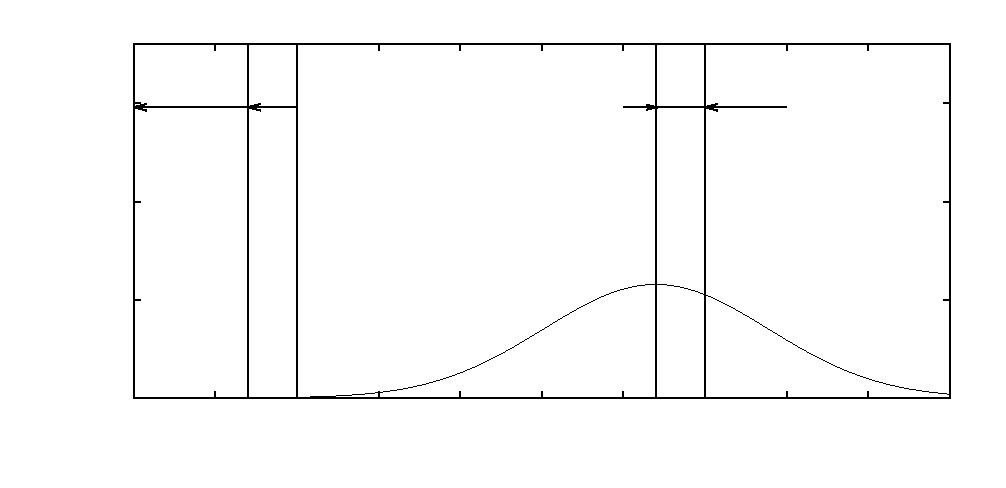
\includegraphics{bell_function_2}}%
    \gplfronttext
  \end{picture}%
\endgroup

		\caption{Probability Calculation}
	\end{figure}
%
To reduce the computing effort of the integration, a transformation is done:
%
	\begin{equation}
		Z=\frac{\Delta v_{z,IMP,crit}-\mu_{v_{z,IMP}}(\sigma_{est})}{\sqrt{V(\sigma_{est})}}
	\end{equation}
%
so that integration tables can be used as an approximation of the probability calculation.
%
\subsection{The Predictor's Trigger}
According to the complementary structure of the algorithm, two conditions are evaluated to trigger an alarm. The conditions are running in parallel which is why an alarm is triggered as soon as one condition is completed. The first condition demands the static impact velocity to be inferior to $-10\,[\frac{ft}{sec}]$. In case of fulfillment, an alarm is triggered. In this case boolean one and thus the mean boolean called \textsl{BWARNOUT} are set to.
The second trigger computes the probability of a hard landing using the procedure discussed in the previous section. It covers the cases in which the predicted static impact velocity is superior to $-10\,[\frac{ft}{sec}]$ but a hard landing due to turbulences might occur. If the computed probability exceeds the threshold of five percent, the \textit{second boolean} \textit{(Warn Out Statistical Subtrigger, BWARNOUTSS)} and thus also the \textit{mean boolean} return \texit{true}.\\
All three booleans are defined as system outputs. It enables to trace which trigger and thus which part of the algorithm  released the warning. This way it is possible to accurately analyse the individual performance of the algorithm's components.
\textit{Warn Out Deterministical Subtrigger, BWARNOUTDS}
\chapter{Assessment}
Within this chapter, the performance of the proposed algorithm is measured and discussed. Due to the modular structure of the predictor, the performance of each individual component is first measured before analysing the overall  prediction performance.
%
\section{Performance of the deterministic estimation}
The algorithm's deterministic part targets the precise calculation of the touchdown velocity $v_{z,IMP,0}$ based on the four deterministically influencing parameters that have been elucidated in Chapter 2.\\
The performances of the two proposed deterministic estimators are measured by comparing their outputs to simulation results. An evaluation set, consisting of 5000 data pairs (matching I/O data), is therefore generated under use of \gls{OSMA}. In the set, the four input parameters ($x_1,...,x_4$) are varied within their predetermined operational areas. The estimated outputs of the 5000 input parameter constellations are then computed by both estimators, the analytical formula and the FIS, in order to compare the results. It is important to mention, that turbulences are deactivated, so that the pure deterministic performance can be measured. To facilitate both evaluation and comparision of the algorithms, three Figure of Merits (FoM) are introduced. The first one is the Detection Rate (DR) indicating the percentage of correctly detected hard landings. For categorisation of the wrong predictions, it is seperated between the Fault Alarm Rate (FAR) which is the 	ratio between the fault Alarms and the total number of observed cases, and the Missed Alarm Rate (MAR).\\
In Fig. 4.1 $\&$ 4.2 the estimated touchdown velocities $v_{z,IMP,0}$ are plotted with respect to the corresponding true impact velocity i.e. the simulated touchdown velocity. The main diagonal and two lines at $\widehat{v}_{z,IMP,0}=-10\, [\frac{ft}{sec}]$ and $v_{z,IMP,0}=-10\,[\frac{ft}{sec}]$are added in both figures, to visualise the dispersions of the estimations and thus the FA and MA.\\
\indent The estimations of the analytical formula are strongly scattered which results in a high number of failed predictions i.e FA (second quadrant) and MA (fourth quadrant). Its DR of 49,05 \% is acompanied by a MAR of 7.62 \% and a FAR of 26 \%. The ratio between FA and MA is $[\frac{1}{3}]$. To analyse the cause of the dispersed result, the estimated influence of each individual parameter ($\gamma_{FIP},\gamma_{rwy},V_{gnd}$) on $v_{z,IMP,0}$ is plotted versus the true parameters influence while freezing the remaining parameters to default values.(see Fig. 4.3 to 4.8).
%	
	\begin{figure}[H]
		% GNUPLOT: LaTeX picture with Postscript
\begingroup
  \makeatletter
  \providecommand\color[2][]{%
    \GenericError{(gnuplot) \space\space\space\@spaces}{%
      Package color not loaded in conjunction with
      terminal option `colourtext'%
    }{See the gnuplot documentation for explanation.%
    }{Either use 'blacktext' in gnuplot or load the package
      color.sty in LaTeX.}%
    \renewcommand\color[2][]{}%
  }%
  \providecommand\includegraphics[2][]{%
    \GenericError{(gnuplot) \space\space\space\@spaces}{%
      Package graphicx or graphics not loaded%
    }{See the gnuplot documentation for explanation.%
    }{The gnuplot epslatex terminal needs graphicx.sty or graphics.sty.}%
    \renewcommand\includegraphics[2][]{}%
  }%
  \providecommand\rotatebox[2]{#2}%
  \@ifundefined{ifGPcolor}{%
    \newif\ifGPcolor
    \GPcolorfalse
  }{}%
  \@ifundefined{ifGPblacktext}{%
    \newif\ifGPblacktext
    \GPblacktexttrue
  }{}%
  % define a \g@addto@macro without @ in the name:
  \let\gplgaddtomacro\g@addto@macro
  % define empty templates for all commands taking text:
  \gdef\gplbacktext{}%
  \gdef\gplfronttext{}%
  \makeatother
  \ifGPblacktext
    % no textcolor at all
    \def\colorrgb#1{}%
    \def\colorgray#1{}%
  \else
    % gray or color?
    \ifGPcolor
      \def\colorrgb#1{\color[rgb]{#1}}%
      \def\colorgray#1{\color[gray]{#1}}%
      \expandafter\def\csname LTw\endcsname{\color{white}}%
      \expandafter\def\csname LTb\endcsname{\color{black}}%
      \expandafter\def\csname LTa\endcsname{\color{black}}%
      \expandafter\def\csname LT0\endcsname{\color[rgb]{1,0,0}}%
      \expandafter\def\csname LT1\endcsname{\color[rgb]{0,1,0}}%
      \expandafter\def\csname LT2\endcsname{\color[rgb]{0,0,1}}%
      \expandafter\def\csname LT3\endcsname{\color[rgb]{1,0,1}}%
      \expandafter\def\csname LT4\endcsname{\color[rgb]{0,1,1}}%
      \expandafter\def\csname LT5\endcsname{\color[rgb]{1,1,0}}%
      \expandafter\def\csname LT6\endcsname{\color[rgb]{0,0,0}}%
      \expandafter\def\csname LT7\endcsname{\color[rgb]{1,0.3,0}}%
      \expandafter\def\csname LT8\endcsname{\color[rgb]{0.5,0.5,0.5}}%
    \else
      % gray
      \def\colorrgb#1{\color{black}}%
      \def\colorgray#1{\color[gray]{#1}}%
      \expandafter\def\csname LTw\endcsname{\color{white}}%
      \expandafter\def\csname LTb\endcsname{\color{black}}%
      \expandafter\def\csname LTa\endcsname{\color{black}}%
      \expandafter\def\csname LT0\endcsname{\color{black}}%
      \expandafter\def\csname LT1\endcsname{\color{black}}%
      \expandafter\def\csname LT2\endcsname{\color{black}}%
      \expandafter\def\csname LT3\endcsname{\color{black}}%
      \expandafter\def\csname LT4\endcsname{\color{black}}%
      \expandafter\def\csname LT5\endcsname{\color{black}}%
      \expandafter\def\csname LT6\endcsname{\color{black}}%
      \expandafter\def\csname LT7\endcsname{\color{black}}%
      \expandafter\def\csname LT8\endcsname{\color{black}}%
    \fi
  \fi
  \setlength{\unitlength}{0.0500bp}%
  \begin{picture}(9070.00,3968.00)%
    \gplgaddtomacro\gplbacktext{%
      \csname LTb\endcsname%
      \put(1078,704){\makebox(0,0)[r]{\strut{}-22.5}}%
      \put(1078,1037){\makebox(0,0)[r]{\strut{}-20}}%
      \put(1078,1370){\makebox(0,0)[r]{\strut{}-17.5}}%
      \put(1078,1704){\makebox(0,0)[r]{\strut{}-15}}%
      \put(1078,2037){\makebox(0,0)[r]{\strut{}-12.5}}%
      \put(1078,2370){\makebox(0,0)[r]{\strut{}-10}}%
      \put(1078,2703){\makebox(0,0)[r]{\strut{}-7.5}}%
      \put(1078,3037){\makebox(0,0)[r]{\strut{}-5}}%
      \put(1078,3370){\makebox(0,0)[r]{\strut{}-2.5}}%
      \put(1078,3703){\makebox(0,0)[r]{\strut{} 0}}%
      \put(1210,484){\makebox(0,0){\strut{}-22.5}}%
      \put(2039,484){\makebox(0,0){\strut{}-20}}%
      \put(2868,484){\makebox(0,0){\strut{}-17.5}}%
      \put(3698,484){\makebox(0,0){\strut{}-15}}%
      \put(4527,484){\makebox(0,0){\strut{}-12.5}}%
      \put(5356,484){\makebox(0,0){\strut{}-10}}%
      \put(6185,484){\makebox(0,0){\strut{}-7.5}}%
      \put(7015,484){\makebox(0,0){\strut{}-5}}%
      \put(7844,484){\makebox(0,0){\strut{}-2.5}}%
      \put(8673,484){\makebox(0,0){\strut{} 0}}%
      \csname LTb\endcsname%
      \put(176,2203){\rotatebox{-270}{\makebox(0,0){\strut{}$\,$$\widehat{v}_{z,IMP,0,analytical}$$[\frac{ft}{sec}]$}}}%
      \put(4941,154){\makebox(0,0){\strut{}$\,$$v_{z,IMP,0}$ $[\frac{ft}{sec}]$}}%
      \put(2868,3503){\makebox(0,0)[l]{\strut{}$MAR=26.00\%$}}%
      \put(6285,931){\makebox(0,0)[l]{\strut{}$FAR=7.62\%$}}%
    }%
    \gplgaddtomacro\gplfronttext{%
    }%
    \gplbacktext
    \put(0,0){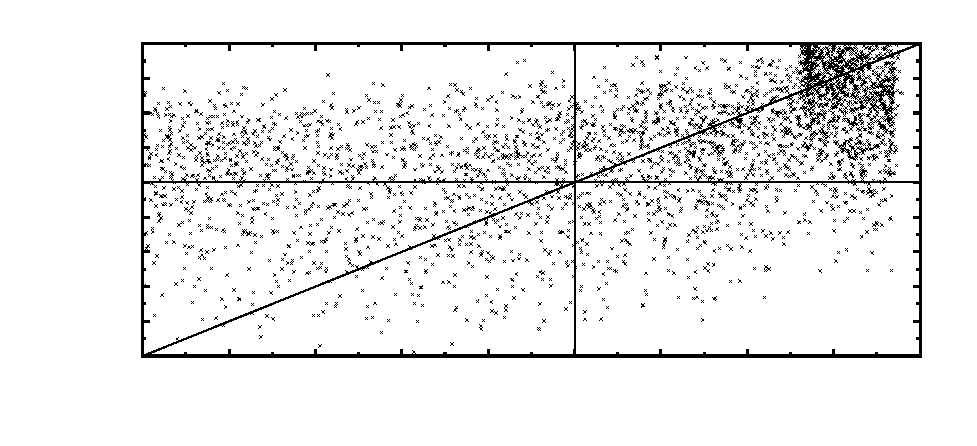
\includegraphics{performance_analytical}}%
    \gplfronttext
  \end{picture}%
\endgroup

		\caption{Analytical Estimation performance}
	\end{figure}
%
%	
	\begin{figure}[H]
		% GNUPLOT: LaTeX picture with Postscript
\begingroup
  \makeatletter
  \providecommand\color[2][]{%
    \GenericError{(gnuplot) \space\space\space\@spaces}{%
      Package color not loaded in conjunction with
      terminal option `colourtext'%
    }{See the gnuplot documentation for explanation.%
    }{Either use 'blacktext' in gnuplot or load the package
      color.sty in LaTeX.}%
    \renewcommand\color[2][]{}%
  }%
  \providecommand\includegraphics[2][]{%
    \GenericError{(gnuplot) \space\space\space\@spaces}{%
      Package graphicx or graphics not loaded%
    }{See the gnuplot documentation for explanation.%
    }{The gnuplot epslatex terminal needs graphicx.sty or graphics.sty.}%
    \renewcommand\includegraphics[2][]{}%
  }%
  \providecommand\rotatebox[2]{#2}%
  \@ifundefined{ifGPcolor}{%
    \newif\ifGPcolor
    \GPcolortrue
  }{}%
  \@ifundefined{ifGPblacktext}{%
    \newif\ifGPblacktext
    \GPblacktexttrue
  }{}%
  % define a \g@addto@macro without @ in the name:
  \let\gplgaddtomacro\g@addto@macro
  % define empty templates for all commands taking text:
  \gdef\gplbacktext{}%
  \gdef\gplfronttext{}%
  \makeatother
  \ifGPblacktext
    % no textcolor at all
    \def\colorrgb#1{}%
    \def\colorgray#1{}%
  \else
    % gray or color?
    \ifGPcolor
      \def\colorrgb#1{\color[rgb]{#1}}%
      \def\colorgray#1{\color[gray]{#1}}%
      \expandafter\def\csname LTw\endcsname{\color{white}}%
      \expandafter\def\csname LTb\endcsname{\color{black}}%
      \expandafter\def\csname LTa\endcsname{\color{black}}%
      \expandafter\def\csname LT0\endcsname{\color[rgb]{1,0,0}}%
      \expandafter\def\csname LT1\endcsname{\color[rgb]{0,1,0}}%
      \expandafter\def\csname LT2\endcsname{\color[rgb]{0,0,1}}%
      \expandafter\def\csname LT3\endcsname{\color[rgb]{1,0,1}}%
      \expandafter\def\csname LT4\endcsname{\color[rgb]{0,1,1}}%
      \expandafter\def\csname LT5\endcsname{\color[rgb]{1,1,0}}%
      \expandafter\def\csname LT6\endcsname{\color[rgb]{0,0,0}}%
      \expandafter\def\csname LT7\endcsname{\color[rgb]{1,0.3,0}}%
      \expandafter\def\csname LT8\endcsname{\color[rgb]{0.5,0.5,0.5}}%
    \else
      % gray
      \def\colorrgb#1{\color{black}}%
      \def\colorgray#1{\color[gray]{#1}}%
      \expandafter\def\csname LTw\endcsname{\color{white}}%
      \expandafter\def\csname LTb\endcsname{\color{black}}%
      \expandafter\def\csname LTa\endcsname{\color{black}}%
      \expandafter\def\csname LT0\endcsname{\color{black}}%
      \expandafter\def\csname LT1\endcsname{\color{black}}%
      \expandafter\def\csname LT2\endcsname{\color{black}}%
      \expandafter\def\csname LT3\endcsname{\color{black}}%
      \expandafter\def\csname LT4\endcsname{\color{black}}%
      \expandafter\def\csname LT5\endcsname{\color{black}}%
      \expandafter\def\csname LT6\endcsname{\color{black}}%
      \expandafter\def\csname LT7\endcsname{\color{black}}%
      \expandafter\def\csname LT8\endcsname{\color{black}}%
    \fi
  \fi
  \setlength{\unitlength}{0.0500bp}%
  \begin{picture}(9070.00,3968.00)%
    \gplgaddtomacro\gplbacktext{%
      \csname LTb\endcsname%
      \put(1078,704){\makebox(0,0)[r]{\strut{}-22.5}}%
      \put(1078,1067){\makebox(0,0)[r]{\strut{}-20}}%
      \put(1078,1429){\makebox(0,0)[r]{\strut{}-17.5}}%
      \put(1078,1792){\makebox(0,0)[r]{\strut{}-15}}%
      \put(1078,2154){\makebox(0,0)[r]{\strut{}-12.5}}%
      \put(1078,2517){\makebox(0,0)[r]{\strut{}-10}}%
      \put(1078,2879){\makebox(0,0)[r]{\strut{}-7.5}}%
      \put(1078,3242){\makebox(0,0)[r]{\strut{}-5}}%
      \put(1078,3604){\makebox(0,0)[r]{\strut{}-2.5}}%
      \put(1078,3967){\makebox(0,0)[r]{\strut{} 0}}%
      \put(1210,484){\makebox(0,0){\strut{}-22.5}}%
      \put(2039,484){\makebox(0,0){\strut{}-20}}%
      \put(2868,484){\makebox(0,0){\strut{}-17.5}}%
      \put(3698,484){\makebox(0,0){\strut{}-15}}%
      \put(4527,484){\makebox(0,0){\strut{}-12.5}}%
      \put(5356,484){\makebox(0,0){\strut{}-10}}%
      \put(6185,484){\makebox(0,0){\strut{}-7.5}}%
      \put(7015,484){\makebox(0,0){\strut{}-5}}%
      \put(7844,484){\makebox(0,0){\strut{}-2.5}}%
      \put(8673,484){\makebox(0,0){\strut{} 0}}%
      \csname LTb\endcsname%
      \put(176,2335){\rotatebox{-270}{\makebox(0,0){\strut{}$\,$$\widehat{v}_{z,IMP,0,fis}$$[\frac{ft}{sec}]$}}}%
      \put(4941,154){\makebox(0,0){\strut{}$\,$$v_{z,IMP,0}$ $[\frac{ft}{sec}]$}}%
      \put(2868,3242){\makebox(0,0)[l]{\strut{}$MAR=0.99\%$}}%
      \put(6285,1647){\makebox(0,0)[l]{\strut{}$FAR=0.92\%$}}%
    }%
    \gplgaddtomacro\gplfronttext{%
    }%
    \gplbacktext
    \put(0,0){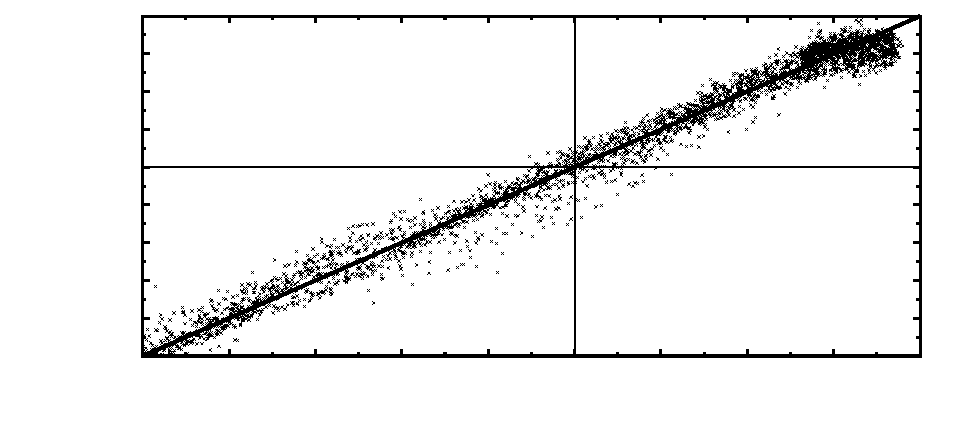
\includegraphics{performance_fis}}%
    \gplfronttext
  \end{picture}%
\endgroup

		\caption{FIS Estimation Performance}
	\end{figure}
%
\newpage
%
\indent \textit{Note: Only parameters enabling a stationary flight ($\gamma_{FIP},\gamma_{rwy},V_{gnd}$) are considered in Fig.4.3 to 4.8, as it is intricate to generate a simulation scenario with an exact instationary initial flight condition whithout influencing the remaining parameters.}
%	
	\begin{figure}[H]
		% GNUPLOT: LaTeX picture with Postscript
\begingroup
  \makeatletter
  \providecommand\color[2][]{%
    \GenericError{(gnuplot) \space\space\space\@spaces}{%
      Package color not loaded in conjunction with
      terminal option `colourtext'%
    }{See the gnuplot documentation for explanation.%
    }{Either use 'blacktext' in gnuplot or load the package
      color.sty in LaTeX.}%
    \renewcommand\color[2][]{}%
  }%
  \providecommand\includegraphics[2][]{%
    \GenericError{(gnuplot) \space\space\space\@spaces}{%
      Package graphicx or graphics not loaded%
    }{See the gnuplot documentation for explanation.%
    }{The gnuplot epslatex terminal needs graphicx.sty or graphics.sty.}%
    \renewcommand\includegraphics[2][]{}%
  }%
  \providecommand\rotatebox[2]{#2}%
  \@ifundefined{ifGPcolor}{%
    \newif\ifGPcolor
    \GPcolortrue
  }{}%
  \@ifundefined{ifGPblacktext}{%
    \newif\ifGPblacktext
    \GPblacktexttrue
  }{}%
  % define a \g@addto@macro without @ in the name:
  \let\gplgaddtomacro\g@addto@macro
  % define empty templates for all commands taking text:
  \gdef\gplbacktext{}%
  \gdef\gplfronttext{}%
  \makeatother
  \ifGPblacktext
    % no textcolor at all
    \def\colorrgb#1{}%
    \def\colorgray#1{}%
  \else
    % gray or color?
    \ifGPcolor
      \def\colorrgb#1{\color[rgb]{#1}}%
      \def\colorgray#1{\color[gray]{#1}}%
      \expandafter\def\csname LTw\endcsname{\color{white}}%
      \expandafter\def\csname LTb\endcsname{\color{black}}%
      \expandafter\def\csname LTa\endcsname{\color{black}}%
      \expandafter\def\csname LT0\endcsname{\color[rgb]{1,0,0}}%
      \expandafter\def\csname LT1\endcsname{\color[rgb]{0,1,0}}%
      \expandafter\def\csname LT2\endcsname{\color[rgb]{0,0,1}}%
      \expandafter\def\csname LT3\endcsname{\color[rgb]{1,0,1}}%
      \expandafter\def\csname LT4\endcsname{\color[rgb]{0,1,1}}%
      \expandafter\def\csname LT5\endcsname{\color[rgb]{1,1,0}}%
      \expandafter\def\csname LT6\endcsname{\color[rgb]{0,0,0}}%
      \expandafter\def\csname LT7\endcsname{\color[rgb]{1,0.3,0}}%
      \expandafter\def\csname LT8\endcsname{\color[rgb]{0.5,0.5,0.5}}%
    \else
      % gray
      \def\colorrgb#1{\color{black}}%
      \def\colorgray#1{\color[gray]{#1}}%
      \expandafter\def\csname LTw\endcsname{\color{white}}%
      \expandafter\def\csname LTb\endcsname{\color{black}}%
      \expandafter\def\csname LTa\endcsname{\color{black}}%
      \expandafter\def\csname LT0\endcsname{\color{black}}%
      \expandafter\def\csname LT1\endcsname{\color{black}}%
      \expandafter\def\csname LT2\endcsname{\color{black}}%
      \expandafter\def\csname LT3\endcsname{\color{black}}%
      \expandafter\def\csname LT4\endcsname{\color{black}}%
      \expandafter\def\csname LT5\endcsname{\color{black}}%
      \expandafter\def\csname LT6\endcsname{\color{black}}%
      \expandafter\def\csname LT7\endcsname{\color{black}}%
      \expandafter\def\csname LT8\endcsname{\color{black}}%
    \fi
  \fi
  \setlength{\unitlength}{0.0500bp}%
  \begin{picture}(9070.00,3400.00)%
    \gplgaddtomacro\gplbacktext{%
      \csname LTb\endcsname%
      \put(814,704){\makebox(0,0)[r]{\strut{}-25}}%
      \csname LTb\endcsname%
      \put(814,1190){\makebox(0,0)[r]{\strut{}-20}}%
      \csname LTb\endcsname%
      \put(814,1676){\makebox(0,0)[r]{\strut{}-15}}%
      \csname LTb\endcsname%
      \put(814,2163){\makebox(0,0)[r]{\strut{}-10}}%
      \csname LTb\endcsname%
      \put(814,2649){\makebox(0,0)[r]{\strut{}-5}}%
      \csname LTb\endcsname%
      \put(814,3135){\makebox(0,0)[r]{\strut{} 0}}%
      \csname LTb\endcsname%
      \put(946,484){\makebox(0,0){\strut{}-5.75}}%
      \csname LTb\endcsname%
      \put(1590,484){\makebox(0,0){\strut{}-5.5}}%
      \csname LTb\endcsname%
      \put(2234,484){\makebox(0,0){\strut{}-5.25}}%
      \csname LTb\endcsname%
      \put(2878,484){\makebox(0,0){\strut{}-5}}%
      \csname LTb\endcsname%
      \put(3522,484){\makebox(0,0){\strut{}-4.75}}%
      \csname LTb\endcsname%
      \put(4166,484){\makebox(0,0){\strut{}-4.5}}%
      \csname LTb\endcsname%
      \put(4809,484){\makebox(0,0){\strut{}-4.25}}%
      \csname LTb\endcsname%
      \put(5453,484){\makebox(0,0){\strut{}-4}}%
      \csname LTb\endcsname%
      \put(6097,484){\makebox(0,0){\strut{}-3.75}}%
      \csname LTb\endcsname%
      \put(6741,484){\makebox(0,0){\strut{}-3.5}}%
      \csname LTb\endcsname%
      \put(7385,484){\makebox(0,0){\strut{}-3.25}}%
      \csname LTb\endcsname%
      \put(8029,484){\makebox(0,0){\strut{}-3}}%
      \csname LTb\endcsname%
      \put(8673,484){\makebox(0,0){\strut{}-2.75}}%
      \put(176,1919){\rotatebox{-270}{\makebox(0,0){\strut{}$v_{z~IMP,0,analytical}\,$$[\frac{ft}{sec}]$}}}%
      \put(4809,154){\makebox(0,0){\strut{}$\gamma_{FIP}[^{\circ}]$}}%
    }%
    \gplgaddtomacro\gplfronttext{%
      \csname LTb\endcsname%
      \put(5517,2934){\makebox(0,0)[r]{\strut{}true impact velocity}}%
      \csname LTb\endcsname%
      \put(5517,2714){\makebox(0,0)[r]{\strut{}estimated impact velocity}}%
    }%
    \gplbacktext
    \put(0,0){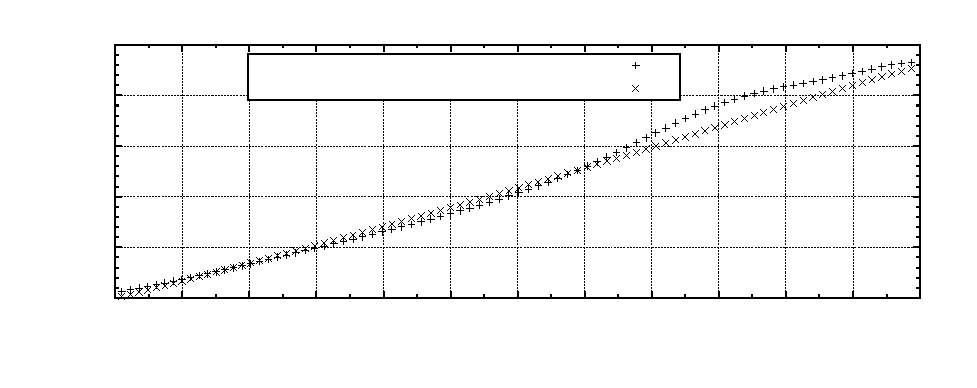
\includegraphics{performance_analytical_GAMGL}}%
    \gplfronttext
  \end{picture}%
\endgroup

		\caption{$\gamma_{FIP}$-Influence - estimated by the Analytical Formula}
	\end{figure}
%
%	
	\begin{figure}[H]
		% GNUPLOT: LaTeX picture with Postscript
\begingroup
  \makeatletter
  \providecommand\color[2][]{%
    \GenericError{(gnuplot) \space\space\space\@spaces}{%
      Package color not loaded in conjunction with
      terminal option `colourtext'%
    }{See the gnuplot documentation for explanation.%
    }{Either use 'blacktext' in gnuplot or load the package
      color.sty in LaTeX.}%
    \renewcommand\color[2][]{}%
  }%
  \providecommand\includegraphics[2][]{%
    \GenericError{(gnuplot) \space\space\space\@spaces}{%
      Package graphicx or graphics not loaded%
    }{See the gnuplot documentation for explanation.%
    }{The gnuplot epslatex terminal needs graphicx.sty or graphics.sty.}%
    \renewcommand\includegraphics[2][]{}%
  }%
  \providecommand\rotatebox[2]{#2}%
  \@ifundefined{ifGPcolor}{%
    \newif\ifGPcolor
    \GPcolortrue
  }{}%
  \@ifundefined{ifGPblacktext}{%
    \newif\ifGPblacktext
    \GPblacktexttrue
  }{}%
  % define a \g@addto@macro without @ in the name:
  \let\gplgaddtomacro\g@addto@macro
  % define empty templates for all commands taking text:
  \gdef\gplbacktext{}%
  \gdef\gplfronttext{}%
  \makeatother
  \ifGPblacktext
    % no textcolor at all
    \def\colorrgb#1{}%
    \def\colorgray#1{}%
  \else
    % gray or color?
    \ifGPcolor
      \def\colorrgb#1{\color[rgb]{#1}}%
      \def\colorgray#1{\color[gray]{#1}}%
      \expandafter\def\csname LTw\endcsname{\color{white}}%
      \expandafter\def\csname LTb\endcsname{\color{black}}%
      \expandafter\def\csname LTa\endcsname{\color{black}}%
      \expandafter\def\csname LT0\endcsname{\color[rgb]{1,0,0}}%
      \expandafter\def\csname LT1\endcsname{\color[rgb]{0,1,0}}%
      \expandafter\def\csname LT2\endcsname{\color[rgb]{0,0,1}}%
      \expandafter\def\csname LT3\endcsname{\color[rgb]{1,0,1}}%
      \expandafter\def\csname LT4\endcsname{\color[rgb]{0,1,1}}%
      \expandafter\def\csname LT5\endcsname{\color[rgb]{1,1,0}}%
      \expandafter\def\csname LT6\endcsname{\color[rgb]{0,0,0}}%
      \expandafter\def\csname LT7\endcsname{\color[rgb]{1,0.3,0}}%
      \expandafter\def\csname LT8\endcsname{\color[rgb]{0.5,0.5,0.5}}%
    \else
      % gray
      \def\colorrgb#1{\color{black}}%
      \def\colorgray#1{\color[gray]{#1}}%
      \expandafter\def\csname LTw\endcsname{\color{white}}%
      \expandafter\def\csname LTb\endcsname{\color{black}}%
      \expandafter\def\csname LTa\endcsname{\color{black}}%
      \expandafter\def\csname LT0\endcsname{\color{black}}%
      \expandafter\def\csname LT1\endcsname{\color{black}}%
      \expandafter\def\csname LT2\endcsname{\color{black}}%
      \expandafter\def\csname LT3\endcsname{\color{black}}%
      \expandafter\def\csname LT4\endcsname{\color{black}}%
      \expandafter\def\csname LT5\endcsname{\color{black}}%
      \expandafter\def\csname LT6\endcsname{\color{black}}%
      \expandafter\def\csname LT7\endcsname{\color{black}}%
      \expandafter\def\csname LT8\endcsname{\color{black}}%
    \fi
  \fi
  \setlength{\unitlength}{0.0500bp}%
  \begin{picture}(9070.00,3400.00)%
    \gplgaddtomacro\gplbacktext{%
      \csname LTb\endcsname%
      \put(946,1109){\makebox(0,0)[r]{\strut{}-5}}%
      \csname LTb\endcsname%
      \put(946,2122){\makebox(0,0)[r]{\strut{}-2.5}}%
      \csname LTb\endcsname%
      \put(946,3135){\makebox(0,0)[r]{\strut{} 0}}%
      \csname LTb\endcsname%
      \put(1315,484){\makebox(0,0){\strut{}-0.75}}%
      \csname LTb\endcsname%
      \put(2502,484){\makebox(0,0){\strut{}-0.5}}%
      \csname LTb\endcsname%
      \put(3689,484){\makebox(0,0){\strut{}-0.25}}%
      \csname LTb\endcsname%
      \put(4876,484){\makebox(0,0){\strut{} 0}}%
      \csname LTb\endcsname%
      \put(6062,484){\makebox(0,0){\strut{} 0.25}}%
      \csname LTb\endcsname%
      \put(7249,484){\makebox(0,0){\strut{} 0.5}}%
      \csname LTb\endcsname%
      \put(8436,484){\makebox(0,0){\strut{} 0.75}}%
      \put(176,1919){\rotatebox{-270}{\makebox(0,0){\strut{}$v_{z~IMP,0,analytical}\,$$[\frac{ft}{sec}]$}}}%
      \put(4875,154){\makebox(0,0){\strut{}Runway Slope [$\%$]}}%
    }%
    \gplgaddtomacro\gplfronttext{%
      \csname LTb\endcsname%
      \put(7686,2962){\makebox(0,0)[r]{\strut{}true impact velocity}}%
      \csname LTb\endcsname%
      \put(7686,2742){\makebox(0,0)[r]{\strut{}estimated impact velocity}}%
    }%
    \gplbacktext
    \put(0,0){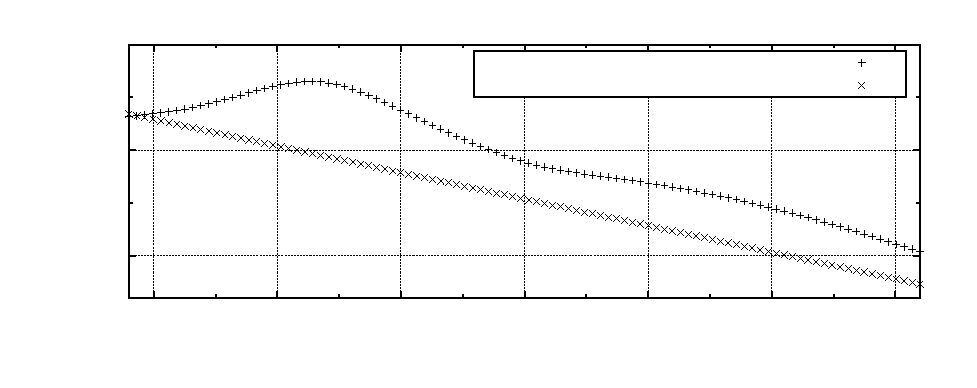
\includegraphics{performance_analytical_GAMPIST}}%
    \gplfronttext
  \end{picture}%
\endgroup

		\caption{Runway Slope Influence - estimated by the Analytical Formula}
	\end{figure}
%
%	
	\begin{figure}[H]
		% GNUPLOT: LaTeX picture with Postscript
\begingroup
  \makeatletter
  \providecommand\color[2][]{%
    \GenericError{(gnuplot) \space\space\space\@spaces}{%
      Package color not loaded in conjunction with
      terminal option `colourtext'%
    }{See the gnuplot documentation for explanation.%
    }{Either use 'blacktext' in gnuplot or load the package
      color.sty in LaTeX.}%
    \renewcommand\color[2][]{}%
  }%
  \providecommand\includegraphics[2][]{%
    \GenericError{(gnuplot) \space\space\space\@spaces}{%
      Package graphicx or graphics not loaded%
    }{See the gnuplot documentation for explanation.%
    }{The gnuplot epslatex terminal needs graphicx.sty or graphics.sty.}%
    \renewcommand\includegraphics[2][]{}%
  }%
  \providecommand\rotatebox[2]{#2}%
  \@ifundefined{ifGPcolor}{%
    \newif\ifGPcolor
    \GPcolortrue
  }{}%
  \@ifundefined{ifGPblacktext}{%
    \newif\ifGPblacktext
    \GPblacktexttrue
  }{}%
  % define a \g@addto@macro without @ in the name:
  \let\gplgaddtomacro\g@addto@macro
  % define empty templates for all commands taking text:
  \gdef\gplbacktext{}%
  \gdef\gplfronttext{}%
  \makeatother
  \ifGPblacktext
    % no textcolor at all
    \def\colorrgb#1{}%
    \def\colorgray#1{}%
  \else
    % gray or color?
    \ifGPcolor
      \def\colorrgb#1{\color[rgb]{#1}}%
      \def\colorgray#1{\color[gray]{#1}}%
      \expandafter\def\csname LTw\endcsname{\color{white}}%
      \expandafter\def\csname LTb\endcsname{\color{black}}%
      \expandafter\def\csname LTa\endcsname{\color{black}}%
      \expandafter\def\csname LT0\endcsname{\color[rgb]{1,0,0}}%
      \expandafter\def\csname LT1\endcsname{\color[rgb]{0,1,0}}%
      \expandafter\def\csname LT2\endcsname{\color[rgb]{0,0,1}}%
      \expandafter\def\csname LT3\endcsname{\color[rgb]{1,0,1}}%
      \expandafter\def\csname LT4\endcsname{\color[rgb]{0,1,1}}%
      \expandafter\def\csname LT5\endcsname{\color[rgb]{1,1,0}}%
      \expandafter\def\csname LT6\endcsname{\color[rgb]{0,0,0}}%
      \expandafter\def\csname LT7\endcsname{\color[rgb]{1,0.3,0}}%
      \expandafter\def\csname LT8\endcsname{\color[rgb]{0.5,0.5,0.5}}%
    \else
      % gray
      \def\colorrgb#1{\color{black}}%
      \def\colorgray#1{\color[gray]{#1}}%
      \expandafter\def\csname LTw\endcsname{\color{white}}%
      \expandafter\def\csname LTb\endcsname{\color{black}}%
      \expandafter\def\csname LTa\endcsname{\color{black}}%
      \expandafter\def\csname LT0\endcsname{\color{black}}%
      \expandafter\def\csname LT1\endcsname{\color{black}}%
      \expandafter\def\csname LT2\endcsname{\color{black}}%
      \expandafter\def\csname LT3\endcsname{\color{black}}%
      \expandafter\def\csname LT4\endcsname{\color{black}}%
      \expandafter\def\csname LT5\endcsname{\color{black}}%
      \expandafter\def\csname LT6\endcsname{\color{black}}%
      \expandafter\def\csname LT7\endcsname{\color{black}}%
      \expandafter\def\csname LT8\endcsname{\color{black}}%
    \fi
  \fi
  \setlength{\unitlength}{0.0500bp}%
  \begin{picture}(9070.00,3400.00)%
    \gplgaddtomacro\gplbacktext{%
      \csname LTb\endcsname%
      \put(682,704){\makebox(0,0)[r]{\strut{}-6}}%
      \csname LTb\endcsname%
      \put(682,1109){\makebox(0,0)[r]{\strut{}-5}}%
      \csname LTb\endcsname%
      \put(682,1514){\makebox(0,0)[r]{\strut{}-4}}%
      \csname LTb\endcsname%
      \put(682,1920){\makebox(0,0)[r]{\strut{}-3}}%
      \csname LTb\endcsname%
      \put(682,2325){\makebox(0,0)[r]{\strut{}-2}}%
      \csname LTb\endcsname%
      \put(682,2730){\makebox(0,0)[r]{\strut{}-1}}%
      \csname LTb\endcsname%
      \put(682,3135){\makebox(0,0)[r]{\strut{} 0}}%
      \csname LTb\endcsname%
      \put(1528,484){\makebox(0,0){\strut{} 120}}%
      \csname LTb\endcsname%
      \put(2957,484){\makebox(0,0){\strut{} 130}}%
      \csname LTb\endcsname%
      \put(4386,484){\makebox(0,0){\strut{} 140}}%
      \csname LTb\endcsname%
      \put(5815,484){\makebox(0,0){\strut{} 150}}%
      \csname LTb\endcsname%
      \put(7244,484){\makebox(0,0){\strut{} 160}}%
      \csname LTb\endcsname%
      \put(8673,484){\makebox(0,0){\strut{} 170}}%
      \put(176,1919){\rotatebox{-270}{\makebox(0,0){\strut{}$v_{z~IMP,0,analytical}\,$\,$[\frac{ft}{sec}]$}}}%
      \put(4743,154){\makebox(0,0){\strut{}$V_{gnd}$\,[kt]}}%
    }%
    \gplgaddtomacro\gplfronttext{%
      \csname LTb\endcsname%
      \put(7686,2962){\makebox(0,0)[r]{\strut{}true impact velocity}}%
      \csname LTb\endcsname%
      \put(7686,2742){\makebox(0,0)[r]{\strut{}estimated impact velocity}}%
    }%
    \gplbacktext
    \put(0,0){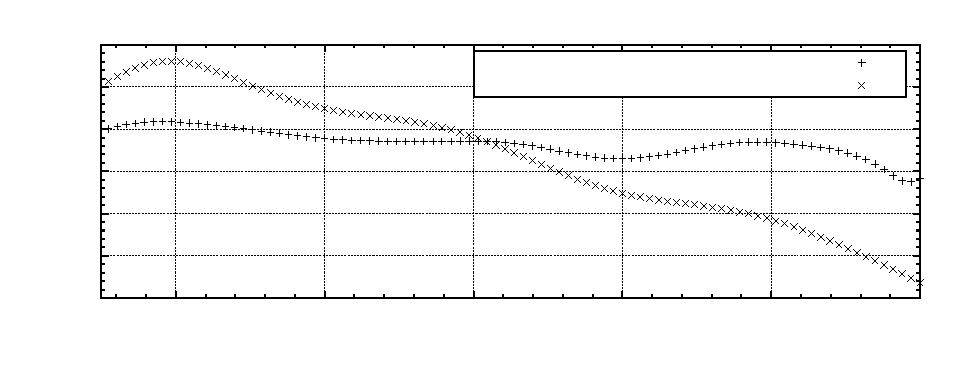
\includegraphics{performance_analytical_V_GND}}%
    \gplfronttext
  \end{picture}%
\endgroup

		\caption{Ground Velocity Influence - estimated by the Analytical Formula}
	\end{figure}
%
%	
	\begin{figure}[H]
		% GNUPLOT: LaTeX picture with Postscript
\begingroup
  \makeatletter
  \providecommand\color[2][]{%
    \GenericError{(gnuplot) \space\space\space\@spaces}{%
      Package color not loaded in conjunction with
      terminal option `colourtext'%
    }{See the gnuplot documentation for explanation.%
    }{Either use 'blacktext' in gnuplot or load the package
      color.sty in LaTeX.}%
    \renewcommand\color[2][]{}%
  }%
  \providecommand\includegraphics[2][]{%
    \GenericError{(gnuplot) \space\space\space\@spaces}{%
      Package graphicx or graphics not loaded%
    }{See the gnuplot documentation for explanation.%
    }{The gnuplot epslatex terminal needs graphicx.sty or graphics.sty.}%
    \renewcommand\includegraphics[2][]{}%
  }%
  \providecommand\rotatebox[2]{#2}%
  \@ifundefined{ifGPcolor}{%
    \newif\ifGPcolor
    \GPcolortrue
  }{}%
  \@ifundefined{ifGPblacktext}{%
    \newif\ifGPblacktext
    \GPblacktexttrue
  }{}%
  % define a \g@addto@macro without @ in the name:
  \let\gplgaddtomacro\g@addto@macro
  % define empty templates for all commands taking text:
  \gdef\gplbacktext{}%
  \gdef\gplfronttext{}%
  \makeatother
  \ifGPblacktext
    % no textcolor at all
    \def\colorrgb#1{}%
    \def\colorgray#1{}%
  \else
    % gray or color?
    \ifGPcolor
      \def\colorrgb#1{\color[rgb]{#1}}%
      \def\colorgray#1{\color[gray]{#1}}%
      \expandafter\def\csname LTw\endcsname{\color{white}}%
      \expandafter\def\csname LTb\endcsname{\color{black}}%
      \expandafter\def\csname LTa\endcsname{\color{black}}%
      \expandafter\def\csname LT0\endcsname{\color[rgb]{1,0,0}}%
      \expandafter\def\csname LT1\endcsname{\color[rgb]{0,1,0}}%
      \expandafter\def\csname LT2\endcsname{\color[rgb]{0,0,1}}%
      \expandafter\def\csname LT3\endcsname{\color[rgb]{1,0,1}}%
      \expandafter\def\csname LT4\endcsname{\color[rgb]{0,1,1}}%
      \expandafter\def\csname LT5\endcsname{\color[rgb]{1,1,0}}%
      \expandafter\def\csname LT6\endcsname{\color[rgb]{0,0,0}}%
      \expandafter\def\csname LT7\endcsname{\color[rgb]{1,0.3,0}}%
      \expandafter\def\csname LT8\endcsname{\color[rgb]{0.5,0.5,0.5}}%
    \else
      % gray
      \def\colorrgb#1{\color{black}}%
      \def\colorgray#1{\color[gray]{#1}}%
      \expandafter\def\csname LTw\endcsname{\color{white}}%
      \expandafter\def\csname LTb\endcsname{\color{black}}%
      \expandafter\def\csname LTa\endcsname{\color{black}}%
      \expandafter\def\csname LT0\endcsname{\color{black}}%
      \expandafter\def\csname LT1\endcsname{\color{black}}%
      \expandafter\def\csname LT2\endcsname{\color{black}}%
      \expandafter\def\csname LT3\endcsname{\color{black}}%
      \expandafter\def\csname LT4\endcsname{\color{black}}%
      \expandafter\def\csname LT5\endcsname{\color{black}}%
      \expandafter\def\csname LT6\endcsname{\color{black}}%
      \expandafter\def\csname LT7\endcsname{\color{black}}%
      \expandafter\def\csname LT8\endcsname{\color{black}}%
    \fi
  \fi
  \setlength{\unitlength}{0.0500bp}%
  \begin{picture}(9070.00,3400.00)%
    \gplgaddtomacro\gplbacktext{%
      \csname LTb\endcsname%
      \put(814,704){\makebox(0,0)[r]{\strut{}-25}}%
      \csname LTb\endcsname%
      \put(814,1190){\makebox(0,0)[r]{\strut{}-20}}%
      \csname LTb\endcsname%
      \put(814,1676){\makebox(0,0)[r]{\strut{}-15}}%
      \csname LTb\endcsname%
      \put(814,2163){\makebox(0,0)[r]{\strut{}-10}}%
      \csname LTb\endcsname%
      \put(814,2649){\makebox(0,0)[r]{\strut{}-5}}%
      \csname LTb\endcsname%
      \put(814,3135){\makebox(0,0)[r]{\strut{} 0}}%
      \csname LTb\endcsname%
      \put(946,484){\makebox(0,0){\strut{}-5.75}}%
      \csname LTb\endcsname%
      \put(1590,484){\makebox(0,0){\strut{}-5.5}}%
      \csname LTb\endcsname%
      \put(2234,484){\makebox(0,0){\strut{}-5.25}}%
      \csname LTb\endcsname%
      \put(2878,484){\makebox(0,0){\strut{}-5}}%
      \csname LTb\endcsname%
      \put(3522,484){\makebox(0,0){\strut{}-4.75}}%
      \csname LTb\endcsname%
      \put(4166,484){\makebox(0,0){\strut{}-4.5}}%
      \csname LTb\endcsname%
      \put(4809,484){\makebox(0,0){\strut{}-4.25}}%
      \csname LTb\endcsname%
      \put(5453,484){\makebox(0,0){\strut{}-4}}%
      \csname LTb\endcsname%
      \put(6097,484){\makebox(0,0){\strut{}-3.75}}%
      \csname LTb\endcsname%
      \put(6741,484){\makebox(0,0){\strut{}-3.5}}%
      \csname LTb\endcsname%
      \put(7385,484){\makebox(0,0){\strut{}-3.25}}%
      \csname LTb\endcsname%
      \put(8029,484){\makebox(0,0){\strut{}-3}}%
      \csname LTb\endcsname%
      \put(8673,484){\makebox(0,0){\strut{}-2.75}}%
      \put(176,1919){\rotatebox{-270}{\makebox(0,0){\strut{}$v_{z~IMP,0,fis}\,$$[\frac{ft}{sec}]$}}}%
      \put(4809,154){\makebox(0,0){\strut{}$\gamma_{FIP}\,[^{\circ}]$}}%
    }%
    \gplgaddtomacro\gplfronttext{%
      \csname LTb\endcsname%
      \put(5517,2934){\makebox(0,0)[r]{\strut{}true impact velocity}}%
      \csname LTb\endcsname%
      \put(5517,2714){\makebox(0,0)[r]{\strut{}estimated impact velocity}}%
    }%
    \gplbacktext
    \put(0,0){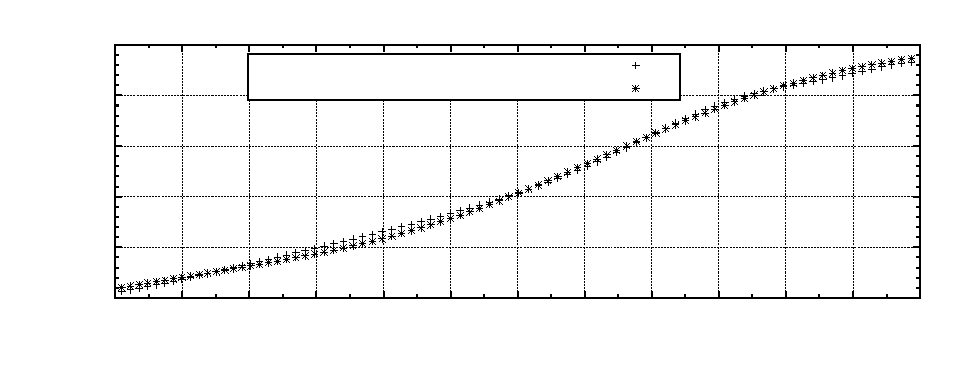
\includegraphics{performance_fis_GAMGL}}%
    \gplfronttext
  \end{picture}%
\endgroup

		\caption{$\gamma_{FIP}$-Influence - estimated by the FIS}
	\end{figure}
%
%	
	\begin{figure}[H]
		% GNUPLOT: LaTeX picture with Postscript
\begingroup
  \makeatletter
  \providecommand\color[2][]{%
    \GenericError{(gnuplot) \space\space\space\@spaces}{%
      Package color not loaded in conjunction with
      terminal option `colourtext'%
    }{See the gnuplot documentation for explanation.%
    }{Either use 'blacktext' in gnuplot or load the package
      color.sty in LaTeX.}%
    \renewcommand\color[2][]{}%
  }%
  \providecommand\includegraphics[2][]{%
    \GenericError{(gnuplot) \space\space\space\@spaces}{%
      Package graphicx or graphics not loaded%
    }{See the gnuplot documentation for explanation.%
    }{The gnuplot epslatex terminal needs graphicx.sty or graphics.sty.}%
    \renewcommand\includegraphics[2][]{}%
  }%
  \providecommand\rotatebox[2]{#2}%
  \@ifundefined{ifGPcolor}{%
    \newif\ifGPcolor
    \GPcolortrue
  }{}%
  \@ifundefined{ifGPblacktext}{%
    \newif\ifGPblacktext
    \GPblacktexttrue
  }{}%
  % define a \g@addto@macro without @ in the name:
  \let\gplgaddtomacro\g@addto@macro
  % define empty templates for all commands taking text:
  \gdef\gplbacktext{}%
  \gdef\gplfronttext{}%
  \makeatother
  \ifGPblacktext
    % no textcolor at all
    \def\colorrgb#1{}%
    \def\colorgray#1{}%
  \else
    % gray or color?
    \ifGPcolor
      \def\colorrgb#1{\color[rgb]{#1}}%
      \def\colorgray#1{\color[gray]{#1}}%
      \expandafter\def\csname LTw\endcsname{\color{white}}%
      \expandafter\def\csname LTb\endcsname{\color{black}}%
      \expandafter\def\csname LTa\endcsname{\color{black}}%
      \expandafter\def\csname LT0\endcsname{\color[rgb]{1,0,0}}%
      \expandafter\def\csname LT1\endcsname{\color[rgb]{0,1,0}}%
      \expandafter\def\csname LT2\endcsname{\color[rgb]{0,0,1}}%
      \expandafter\def\csname LT3\endcsname{\color[rgb]{1,0,1}}%
      \expandafter\def\csname LT4\endcsname{\color[rgb]{0,1,1}}%
      \expandafter\def\csname LT5\endcsname{\color[rgb]{1,1,0}}%
      \expandafter\def\csname LT6\endcsname{\color[rgb]{0,0,0}}%
      \expandafter\def\csname LT7\endcsname{\color[rgb]{1,0.3,0}}%
      \expandafter\def\csname LT8\endcsname{\color[rgb]{0.5,0.5,0.5}}%
    \else
      % gray
      \def\colorrgb#1{\color{black}}%
      \def\colorgray#1{\color[gray]{#1}}%
      \expandafter\def\csname LTw\endcsname{\color{white}}%
      \expandafter\def\csname LTb\endcsname{\color{black}}%
      \expandafter\def\csname LTa\endcsname{\color{black}}%
      \expandafter\def\csname LT0\endcsname{\color{black}}%
      \expandafter\def\csname LT1\endcsname{\color{black}}%
      \expandafter\def\csname LT2\endcsname{\color{black}}%
      \expandafter\def\csname LT3\endcsname{\color{black}}%
      \expandafter\def\csname LT4\endcsname{\color{black}}%
      \expandafter\def\csname LT5\endcsname{\color{black}}%
      \expandafter\def\csname LT6\endcsname{\color{black}}%
      \expandafter\def\csname LT7\endcsname{\color{black}}%
      \expandafter\def\csname LT8\endcsname{\color{black}}%
    \fi
  \fi
  \setlength{\unitlength}{0.0500bp}%
  \begin{picture}(9070.00,3400.00)%
    \gplgaddtomacro\gplbacktext{%
      \csname LTb\endcsname%
      \put(946,1109){\makebox(0,0)[r]{\strut{}-5}}%
      \csname LTb\endcsname%
      \put(946,2122){\makebox(0,0)[r]{\strut{}-2.5}}%
      \csname LTb\endcsname%
      \put(946,3135){\makebox(0,0)[r]{\strut{} 0}}%
      \csname LTb\endcsname%
      \put(1315,484){\makebox(0,0){\strut{}-0.75}}%
      \csname LTb\endcsname%
      \put(2502,484){\makebox(0,0){\strut{}-0.5}}%
      \csname LTb\endcsname%
      \put(3689,484){\makebox(0,0){\strut{}-0.25}}%
      \csname LTb\endcsname%
      \put(4876,484){\makebox(0,0){\strut{} 0}}%
      \csname LTb\endcsname%
      \put(6062,484){\makebox(0,0){\strut{} 0.25}}%
      \csname LTb\endcsname%
      \put(7249,484){\makebox(0,0){\strut{} 0.5}}%
      \csname LTb\endcsname%
      \put(8436,484){\makebox(0,0){\strut{} 0.75}}%
      \put(176,1919){\rotatebox{-270}{\makebox(0,0){\strut{}$v_{z~IMP,0,FIS}\,$$[\frac{ft}{sec}]$}}}%
      \put(4875,154){\makebox(0,0){\strut{}Runway Slope [$\%$]}}%
    }%
    \gplgaddtomacro\gplfronttext{%
      \csname LTb\endcsname%
      \put(7686,2962){\makebox(0,0)[r]{\strut{}true impact velocity}}%
      \csname LTb\endcsname%
      \put(7686,2742){\makebox(0,0)[r]{\strut{}estimated impact velocity}}%
    }%
    \gplbacktext
    \put(0,0){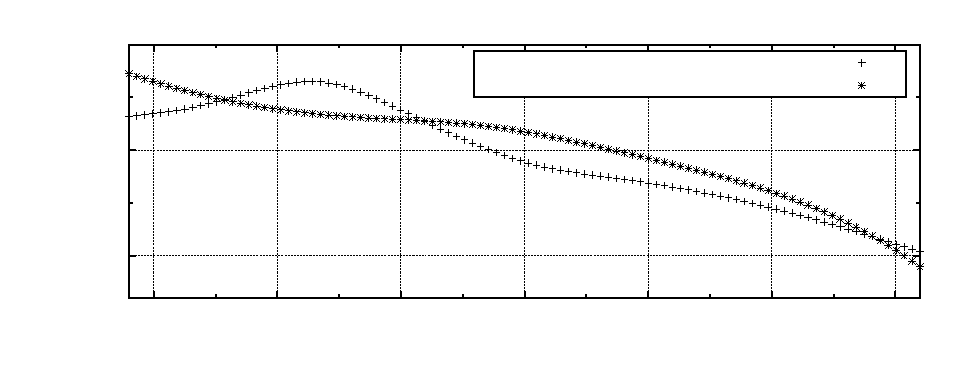
\includegraphics{performance_fis_GAMPIST}}%
    \gplfronttext
  \end{picture}%
\endgroup

		\caption{Runway Slope Influence - estimated by the FIS}
	\end{figure}
%
%	
	\begin{figure}[H]
		% GNUPLOT: LaTeX picture with Postscript
\begingroup
  \makeatletter
  \providecommand\color[2][]{%
    \GenericError{(gnuplot) \space\space\space\@spaces}{%
      Package color not loaded in conjunction with
      terminal option `colourtext'%
    }{See the gnuplot documentation for explanation.%
    }{Either use 'blacktext' in gnuplot or load the package
      color.sty in LaTeX.}%
    \renewcommand\color[2][]{}%
  }%
  \providecommand\includegraphics[2][]{%
    \GenericError{(gnuplot) \space\space\space\@spaces}{%
      Package graphicx or graphics not loaded%
    }{See the gnuplot documentation for explanation.%
    }{The gnuplot epslatex terminal needs graphicx.sty or graphics.sty.}%
    \renewcommand\includegraphics[2][]{}%
  }%
  \providecommand\rotatebox[2]{#2}%
  \@ifundefined{ifGPcolor}{%
    \newif\ifGPcolor
    \GPcolortrue
  }{}%
  \@ifundefined{ifGPblacktext}{%
    \newif\ifGPblacktext
    \GPblacktexttrue
  }{}%
  % define a \g@addto@macro without @ in the name:
  \let\gplgaddtomacro\g@addto@macro
  % define empty templates for all commands taking text:
  \gdef\gplbacktext{}%
  \gdef\gplfronttext{}%
  \makeatother
  \ifGPblacktext
    % no textcolor at all
    \def\colorrgb#1{}%
    \def\colorgray#1{}%
  \else
    % gray or color?
    \ifGPcolor
      \def\colorrgb#1{\color[rgb]{#1}}%
      \def\colorgray#1{\color[gray]{#1}}%
      \expandafter\def\csname LTw\endcsname{\color{white}}%
      \expandafter\def\csname LTb\endcsname{\color{black}}%
      \expandafter\def\csname LTa\endcsname{\color{black}}%
      \expandafter\def\csname LT0\endcsname{\color[rgb]{1,0,0}}%
      \expandafter\def\csname LT1\endcsname{\color[rgb]{0,1,0}}%
      \expandafter\def\csname LT2\endcsname{\color[rgb]{0,0,1}}%
      \expandafter\def\csname LT3\endcsname{\color[rgb]{1,0,1}}%
      \expandafter\def\csname LT4\endcsname{\color[rgb]{0,1,1}}%
      \expandafter\def\csname LT5\endcsname{\color[rgb]{1,1,0}}%
      \expandafter\def\csname LT6\endcsname{\color[rgb]{0,0,0}}%
      \expandafter\def\csname LT7\endcsname{\color[rgb]{1,0.3,0}}%
      \expandafter\def\csname LT8\endcsname{\color[rgb]{0.5,0.5,0.5}}%
    \else
      % gray
      \def\colorrgb#1{\color{black}}%
      \def\colorgray#1{\color[gray]{#1}}%
      \expandafter\def\csname LTw\endcsname{\color{white}}%
      \expandafter\def\csname LTb\endcsname{\color{black}}%
      \expandafter\def\csname LTa\endcsname{\color{black}}%
      \expandafter\def\csname LT0\endcsname{\color{black}}%
      \expandafter\def\csname LT1\endcsname{\color{black}}%
      \expandafter\def\csname LT2\endcsname{\color{black}}%
      \expandafter\def\csname LT3\endcsname{\color{black}}%
      \expandafter\def\csname LT4\endcsname{\color{black}}%
      \expandafter\def\csname LT5\endcsname{\color{black}}%
      \expandafter\def\csname LT6\endcsname{\color{black}}%
      \expandafter\def\csname LT7\endcsname{\color{black}}%
      \expandafter\def\csname LT8\endcsname{\color{black}}%
    \fi
  \fi
  \setlength{\unitlength}{0.0500bp}%
  \begin{picture}(9070.00,3400.00)%
    \gplgaddtomacro\gplbacktext{%
      \csname LTb\endcsname%
      \put(946,704){\makebox(0,0)[r]{\strut{}-3.5}}%
      \csname LTb\endcsname%
      \put(946,1051){\makebox(0,0)[r]{\strut{}-3}}%
      \csname LTb\endcsname%
      \put(946,1399){\makebox(0,0)[r]{\strut{}-2.5}}%
      \csname LTb\endcsname%
      \put(946,1746){\makebox(0,0)[r]{\strut{}-2}}%
      \csname LTb\endcsname%
      \put(946,2093){\makebox(0,0)[r]{\strut{}-1.5}}%
      \csname LTb\endcsname%
      \put(946,2440){\makebox(0,0)[r]{\strut{}-1}}%
      \csname LTb\endcsname%
      \put(946,2788){\makebox(0,0)[r]{\strut{}-0.5}}%
      \csname LTb\endcsname%
      \put(946,3135){\makebox(0,0)[r]{\strut{} 0}}%
      \csname LTb\endcsname%
      \put(2459,484){\makebox(0,0){\strut{} 125}}%
      \csname LTb\endcsname%
      \put(5911,484){\makebox(0,0){\strut{} 150}}%
      \put(176,1919){\rotatebox{-270}{\makebox(0,0){\strut{}$v_{z~IMP,0,FIS}\,$\,$[\frac{ft}{sec}]$}}}%
      \put(4875,154){\makebox(0,0){\strut{}$V_{gnd}\,$[kt]}}%
    }%
    \gplgaddtomacro\gplfronttext{%
      \csname LTb\endcsname%
      \put(7686,2962){\makebox(0,0)[r]{\strut{}true impact velocity}}%
      \csname LTb\endcsname%
      \put(7686,2742){\makebox(0,0)[r]{\strut{}estimated impact velocity}}%
    }%
    \gplbacktext
    \put(0,0){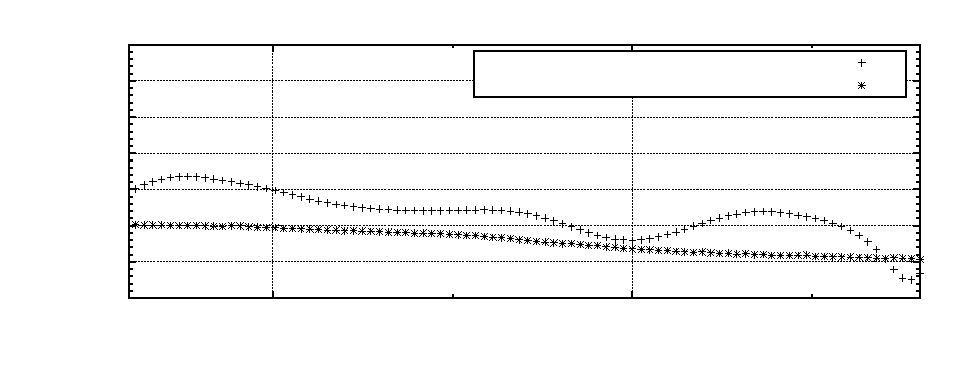
\includegraphics{performance_fis_V_GND}}%
    \gplfronttext
  \end{picture}%
\endgroup

		\caption{Ground Velocity Influence - estimated by the FIS}
	\end{figure}
%
\newpage
%
The dispersions between the true and the estimated values are due to the multiple simplifications the analytical formula contains (see Chapter 3).\\
\indent Contrary to the analytical formula, the FIS' estimations are less scattered (see Fig. 4.2). The FIS' MAR of 0.99 \% and FAR of 0.92 \% is accompanied by a DR of 98.02 \%. The repartition ratio between FA and MA is $[\frac{1}{1}]$. Regarding these performances it is to say, that the model describes the system adequately which is why the dispersion between true and estimated individual parameter influence is almost insignificant. The accurate performance of the fis is not only attributed to the large number of training data pairs that have been introduced in the learning process. The performance is also attributed to the ability of FIS to emulate non-linear system behaviours through decomposition in multiple local linear models.\\
\indent Regarding the large performance discrepancy which has been exposed between the two proposed deterministic estimators, only the FIS is further considered, since the effort to improve the analytical formula's performance in order to reach comparable estimation results is intricate and time consuming rendering it the inferior alternative.\\
\indent To demonstrate the influence that turbulences evoke on the FIS estimation performance, Fig. 4.9 illustrates how the FIS performs under activation of turbulence. Therefore the same scenario as in Fig. 4.1 and 4.2 is used. The plot expresses the the need to build a complementary algorithm, since the estimations are widely scattered and thus unuseful for a prediction. Compared to Fig. 4.2, the DR is reduced to 84 $\%$. The MAR and FAR rise to 7$\%$ and $14\%$.
%	
	\begin{figure}[H]
		% GNUPLOT: LaTeX picture with Postscript
\begingroup
  \makeatletter
  \providecommand\color[2][]{%
    \GenericError{(gnuplot) \space\space\space\@spaces}{%
      Package color not loaded in conjunction with
      terminal option `colourtext'%
    }{See the gnuplot documentation for explanation.%
    }{Either use 'blacktext' in gnuplot or load the package
      color.sty in LaTeX.}%
    \renewcommand\color[2][]{}%
  }%
  \providecommand\includegraphics[2][]{%
    \GenericError{(gnuplot) \space\space\space\@spaces}{%
      Package graphicx or graphics not loaded%
    }{See the gnuplot documentation for explanation.%
    }{The gnuplot epslatex terminal needs graphicx.sty or graphics.sty.}%
    \renewcommand\includegraphics[2][]{}%
  }%
  \providecommand\rotatebox[2]{#2}%
  \@ifundefined{ifGPcolor}{%
    \newif\ifGPcolor
    \GPcolortrue
  }{}%
  \@ifundefined{ifGPblacktext}{%
    \newif\ifGPblacktext
    \GPblacktexttrue
  }{}%
  % define a \g@addto@macro without @ in the name:
  \let\gplgaddtomacro\g@addto@macro
  % define empty templates for all commands taking text:
  \gdef\gplbacktext{}%
  \gdef\gplfronttext{}%
  \makeatother
  \ifGPblacktext
    % no textcolor at all
    \def\colorrgb#1{}%
    \def\colorgray#1{}%
  \else
    % gray or color?
    \ifGPcolor
      \def\colorrgb#1{\color[rgb]{#1}}%
      \def\colorgray#1{\color[gray]{#1}}%
      \expandafter\def\csname LTw\endcsname{\color{white}}%
      \expandafter\def\csname LTb\endcsname{\color{black}}%
      \expandafter\def\csname LTa\endcsname{\color{black}}%
      \expandafter\def\csname LT0\endcsname{\color[rgb]{1,0,0}}%
      \expandafter\def\csname LT1\endcsname{\color[rgb]{0,1,0}}%
      \expandafter\def\csname LT2\endcsname{\color[rgb]{0,0,1}}%
      \expandafter\def\csname LT3\endcsname{\color[rgb]{1,0,1}}%
      \expandafter\def\csname LT4\endcsname{\color[rgb]{0,1,1}}%
      \expandafter\def\csname LT5\endcsname{\color[rgb]{1,1,0}}%
      \expandafter\def\csname LT6\endcsname{\color[rgb]{0,0,0}}%
      \expandafter\def\csname LT7\endcsname{\color[rgb]{1,0.3,0}}%
      \expandafter\def\csname LT8\endcsname{\color[rgb]{0.5,0.5,0.5}}%
    \else
      % gray
      \def\colorrgb#1{\color{black}}%
      \def\colorgray#1{\color[gray]{#1}}%
      \expandafter\def\csname LTw\endcsname{\color{white}}%
      \expandafter\def\csname LTb\endcsname{\color{black}}%
      \expandafter\def\csname LTa\endcsname{\color{black}}%
      \expandafter\def\csname LT0\endcsname{\color{black}}%
      \expandafter\def\csname LT1\endcsname{\color{black}}%
      \expandafter\def\csname LT2\endcsname{\color{black}}%
      \expandafter\def\csname LT3\endcsname{\color{black}}%
      \expandafter\def\csname LT4\endcsname{\color{black}}%
      \expandafter\def\csname LT5\endcsname{\color{black}}%
      \expandafter\def\csname LT6\endcsname{\color{black}}%
      \expandafter\def\csname LT7\endcsname{\color{black}}%
      \expandafter\def\csname LT8\endcsname{\color{black}}%
    \fi
  \fi
  \setlength{\unitlength}{0.0500bp}%
  \begin{picture}(9070.00,4534.00)%
    \gplgaddtomacro\gplbacktext{%
      \csname LTb\endcsname%
      \put(1078,704){\makebox(0,0)[r]{\strut{}-22.5}}%
      \put(1078,1100){\makebox(0,0)[r]{\strut{}-20}}%
      \put(1078,1496){\makebox(0,0)[r]{\strut{}-17.5}}%
      \put(1078,1892){\makebox(0,0)[r]{\strut{}-15}}%
      \put(1078,2288){\makebox(0,0)[r]{\strut{}-12.5}}%
      \put(1078,2685){\makebox(0,0)[r]{\strut{}-10}}%
      \put(1078,3081){\makebox(0,0)[r]{\strut{}-7.5}}%
      \put(1078,3477){\makebox(0,0)[r]{\strut{}-5}}%
      \put(1078,3873){\makebox(0,0)[r]{\strut{}-2.5}}%
      \put(1078,4269){\makebox(0,0)[r]{\strut{} 0}}%
      \put(1210,484){\makebox(0,0){\strut{}-22.5}}%
      \put(2039,484){\makebox(0,0){\strut{}-20}}%
      \put(2868,484){\makebox(0,0){\strut{}-17.5}}%
      \put(3698,484){\makebox(0,0){\strut{}-15}}%
      \put(4527,484){\makebox(0,0){\strut{}-12.5}}%
      \put(5356,484){\makebox(0,0){\strut{}-10}}%
      \put(6185,484){\makebox(0,0){\strut{}-7.5}}%
      \put(7015,484){\makebox(0,0){\strut{}-5}}%
      \put(7844,484){\makebox(0,0){\strut{}-2.5}}%
      \put(8673,484){\makebox(0,0){\strut{} 0}}%
      \csname LTb\endcsname%
      \put(176,2486){\rotatebox{-270}{\makebox(0,0){\strut{}$\,$$\widehat{v}_{z,IMP,0,FIS}$ $[\frac{ft}{sec}]$}}}%
      \put(4941,154){\makebox(0,0){\strut{}$\,$$v_{z,IMP,0}$ $[\frac{ft}{sec}]$}}%
    }%
    \gplgaddtomacro\gplfronttext{%
    }%
    \gplbacktext
    \put(0,0){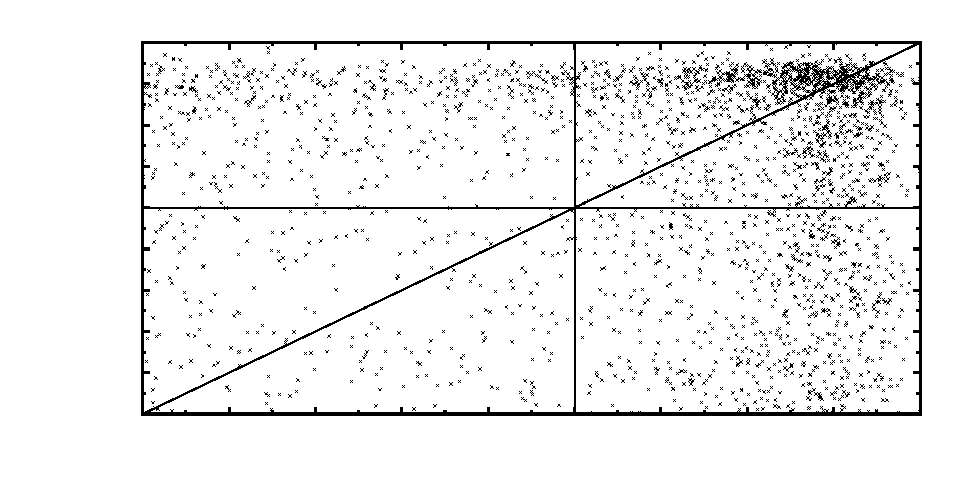
\includegraphics{benefit}}%
    \gplfronttext
  \end{picture}%
\endgroup

		\caption{FIS Performance under Turbulence}
	\end{figure}
%
\section{Turbulence estimation performance}
As described in Chapter 3, the vertical wind velocity has to be observed during the approach i.e before the automatic flare is initiated in order to estimate the turbulence intensity and moreover the probability of a hard landing.\\
In Fig. 4.10, a multiplot illustrates the performance of the turbulence intensity estimator.
%	
	\begin{figure}[H]
		% GNUPLOT: LaTeX picture with Postscript
\begingroup
  \makeatletter
  \providecommand\color[2][]{%
    \GenericError{(gnuplot) \space\space\space\@spaces}{%
      Package color not loaded in conjunction with
      terminal option `colourtext'%
    }{See the gnuplot documentation for explanation.%
    }{Either use 'blacktext' in gnuplot or load the package
      color.sty in LaTeX.}%
    \renewcommand\color[2][]{}%
  }%
  \providecommand\includegraphics[2][]{%
    \GenericError{(gnuplot) \space\space\space\@spaces}{%
      Package graphicx or graphics not loaded%
    }{See the gnuplot documentation for explanation.%
    }{The gnuplot epslatex terminal needs graphicx.sty or graphics.sty.}%
    \renewcommand\includegraphics[2][]{}%
  }%
  \providecommand\rotatebox[2]{#2}%
  \@ifundefined{ifGPcolor}{%
    \newif\ifGPcolor
    \GPcolortrue
  }{}%
  \@ifundefined{ifGPblacktext}{%
    \newif\ifGPblacktext
    \GPblacktexttrue
  }{}%
  % define a \g@addto@macro without @ in the name:
  \let\gplgaddtomacro\g@addto@macro
  % define empty templates for all commands taking text:
  \gdef\gplbacktext{}%
  \gdef\gplfronttext{}%
  \makeatother
  \ifGPblacktext
    % no textcolor at all
    \def\colorrgb#1{}%
    \def\colorgray#1{}%
  \else
    % gray or color?
    \ifGPcolor
      \def\colorrgb#1{\color[rgb]{#1}}%
      \def\colorgray#1{\color[gray]{#1}}%
      \expandafter\def\csname LTw\endcsname{\color{white}}%
      \expandafter\def\csname LTb\endcsname{\color{black}}%
      \expandafter\def\csname LTa\endcsname{\color{black}}%
      \expandafter\def\csname LT0\endcsname{\color[rgb]{1,0,0}}%
      \expandafter\def\csname LT1\endcsname{\color[rgb]{0,1,0}}%
      \expandafter\def\csname LT2\endcsname{\color[rgb]{0,0,1}}%
      \expandafter\def\csname LT3\endcsname{\color[rgb]{1,0,1}}%
      \expandafter\def\csname LT4\endcsname{\color[rgb]{0,1,1}}%
      \expandafter\def\csname LT5\endcsname{\color[rgb]{1,1,0}}%
      \expandafter\def\csname LT6\endcsname{\color[rgb]{0,0,0}}%
      \expandafter\def\csname LT7\endcsname{\color[rgb]{1,0.3,0}}%
      \expandafter\def\csname LT8\endcsname{\color[rgb]{0.5,0.5,0.5}}%
    \else
      % gray
      \def\colorrgb#1{\color{black}}%
      \def\colorgray#1{\color[gray]{#1}}%
      \expandafter\def\csname LTw\endcsname{\color{white}}%
      \expandafter\def\csname LTb\endcsname{\color{black}}%
      \expandafter\def\csname LTa\endcsname{\color{black}}%
      \expandafter\def\csname LT0\endcsname{\color{black}}%
      \expandafter\def\csname LT1\endcsname{\color{black}}%
      \expandafter\def\csname LT2\endcsname{\color{black}}%
      \expandafter\def\csname LT3\endcsname{\color{black}}%
      \expandafter\def\csname LT4\endcsname{\color{black}}%
      \expandafter\def\csname LT5\endcsname{\color{black}}%
      \expandafter\def\csname LT6\endcsname{\color{black}}%
      \expandafter\def\csname LT7\endcsname{\color{black}}%
      \expandafter\def\csname LT8\endcsname{\color{black}}%
    \fi
  \fi
  \setlength{\unitlength}{0.0500bp}%
  \begin{picture}(8502.00,9070.00)%
    \gplgaddtomacro\gplbacktext{%
      \csname LTb\endcsname%
      \put(982,7256){\makebox(0,0)[r]{\strut{} 0}}%
      \put(982,7562){\makebox(0,0)[r]{\strut{} 100}}%
      \put(982,7869){\makebox(0,0)[r]{\strut{} 200}}%
      \put(982,8175){\makebox(0,0)[r]{\strut{} 300}}%
      \put(982,8481){\makebox(0,0)[r]{\strut{} 400}}%
      \put(982,8788){\makebox(0,0)[r]{\strut{} 500}}%
      \put(1114,7036){\makebox(0,0){\strut{}}}%
      \put(2047,7036){\makebox(0,0){\strut{}}}%
      \put(2981,7036){\makebox(0,0){\strut{}}}%
      \put(3914,7036){\makebox(0,0){\strut{}}}%
      \put(4848,7036){\makebox(0,0){\strut{}}}%
      \put(5781,7036){\makebox(0,0){\strut{}}}%
      \put(6715,7036){\makebox(0,0){\strut{}}}%
      \put(7648,7036){\makebox(0,0){\strut{}}}%
      \put(8582,7036){\makebox(0,0){\strut{}}}%
      \put(410,8052){\rotatebox{-270}{\makebox(0,0){\strut{}height[ft]}}}%
      \put(5034,6970){\makebox(0,0){\strut{}}}%
    }%
    \gplgaddtomacro\gplfronttext{%
    }%
    \gplgaddtomacro\gplbacktext{%
      \csname LTb\endcsname%
      \put(982,5442){\makebox(0,0)[r]{\strut{} 0}}%
      \put(982,5975){\makebox(0,0)[r]{\strut{} 0.5}}%
      \put(982,6508){\makebox(0,0)[r]{\strut{} 1}}%
      \put(982,7042){\makebox(0,0)[r]{\strut{} 1.5}}%
      \put(1114,5222){\makebox(0,0){\strut{}}}%
      \put(2047,5222){\makebox(0,0){\strut{}}}%
      \put(2981,5222){\makebox(0,0){\strut{}}}%
      \put(3914,5222){\makebox(0,0){\strut{}}}%
      \put(4848,5222){\makebox(0,0){\strut{}}}%
      \put(5781,5222){\makebox(0,0){\strut{}}}%
      \put(6715,5222){\makebox(0,0){\strut{}}}%
      \put(7648,5222){\makebox(0,0){\strut{}}}%
      \put(8582,5222){\makebox(0,0){\strut{}}}%
      \put(410,6348){\rotatebox{-270}{\makebox(0,0){\strut{}observation[-]}}}%
      \put(5034,5156){\makebox(0,0){\strut{}}}%
    }%
    \gplgaddtomacro\gplfronttext{%
    }%
    \gplgaddtomacro\gplbacktext{%
      \csname LTb\endcsname%
      \put(982,3143){\makebox(0,0)[r]{\strut{}-2}}%
      \put(982,3612){\makebox(0,0)[r]{\strut{}-1}}%
      \put(982,4081){\makebox(0,0)[r]{\strut{} 0}}%
      \put(982,4550){\makebox(0,0)[r]{\strut{} 1}}%
      \put(982,5019){\makebox(0,0)[r]{\strut{} 2}}%
      \put(1114,2501){\makebox(0,0){\strut{}}}%
      \put(2047,2501){\makebox(0,0){\strut{}}}%
      \put(2981,2501){\makebox(0,0){\strut{}}}%
      \put(3914,2501){\makebox(0,0){\strut{}}}%
      \put(4848,2501){\makebox(0,0){\strut{}}}%
      \put(5781,2501){\makebox(0,0){\strut{}}}%
      \put(6715,2501){\makebox(0,0){\strut{}}}%
      \put(7648,2501){\makebox(0,0){\strut{}}}%
      \put(8582,2501){\makebox(0,0){\strut{}}}%
      \put(364,4081){\rotatebox{-270}{\makebox(0,0){\strut{}wind velocity$\,[\frac{m}{s}]$}}}%
      \put(5034,2435){\makebox(0,0){\strut{}}}%
    }%
    \gplgaddtomacro\gplfronttext{%
      \put(7968,5268){\makebox(0,0)[r]{\strut{}estimated wind velocity}}%
      \csname LTb\endcsname%
      \put(7968,5048){\makebox(0,0)[r]{\strut{}true wind velocity}}%
    }%
    \gplgaddtomacro\gplbacktext{%
      \csname LTb\endcsname%
      \put(982,660){\makebox(0,0)[r]{\strut{} 0}}%
      \put(982,2534){\makebox(0,0)[r]{\strut{} 1}}%
      \put(1114,440){\makebox(0,0){\strut{}0}}%
      \put(2047,440){\makebox(0,0){\strut{}5}}%
      \put(2981,440){\makebox(0,0){\strut{}10}}%
      \put(3914,440){\makebox(0,0){\strut{}15}}%
      \put(4848,440){\makebox(0,0){\strut{}20}}%
      \put(5781,440){\makebox(0,0){\strut{}25}}%
      \put(6715,440){\makebox(0,0){\strut{}30}}%
      \put(7648,440){\makebox(0,0){\strut{}35}}%
      \put(8582,440){\makebox(0,0){\strut{}40}}%
      \put(364,1690){\rotatebox{-270}{\makebox(0,0){\strut{}intensity$\,$ $\widehat{\sigma}$[-]}}}%
      \put(5034,110){\makebox(0,0){\strut{}time [sec]}}%
      \put(3914,2477){\makebox(0,0)[l]{\strut{}true turbulence intensity level }}%
    }%
    \gplgaddtomacro\gplfronttext{%
    }%
    \gplbacktext
    \put(0,0){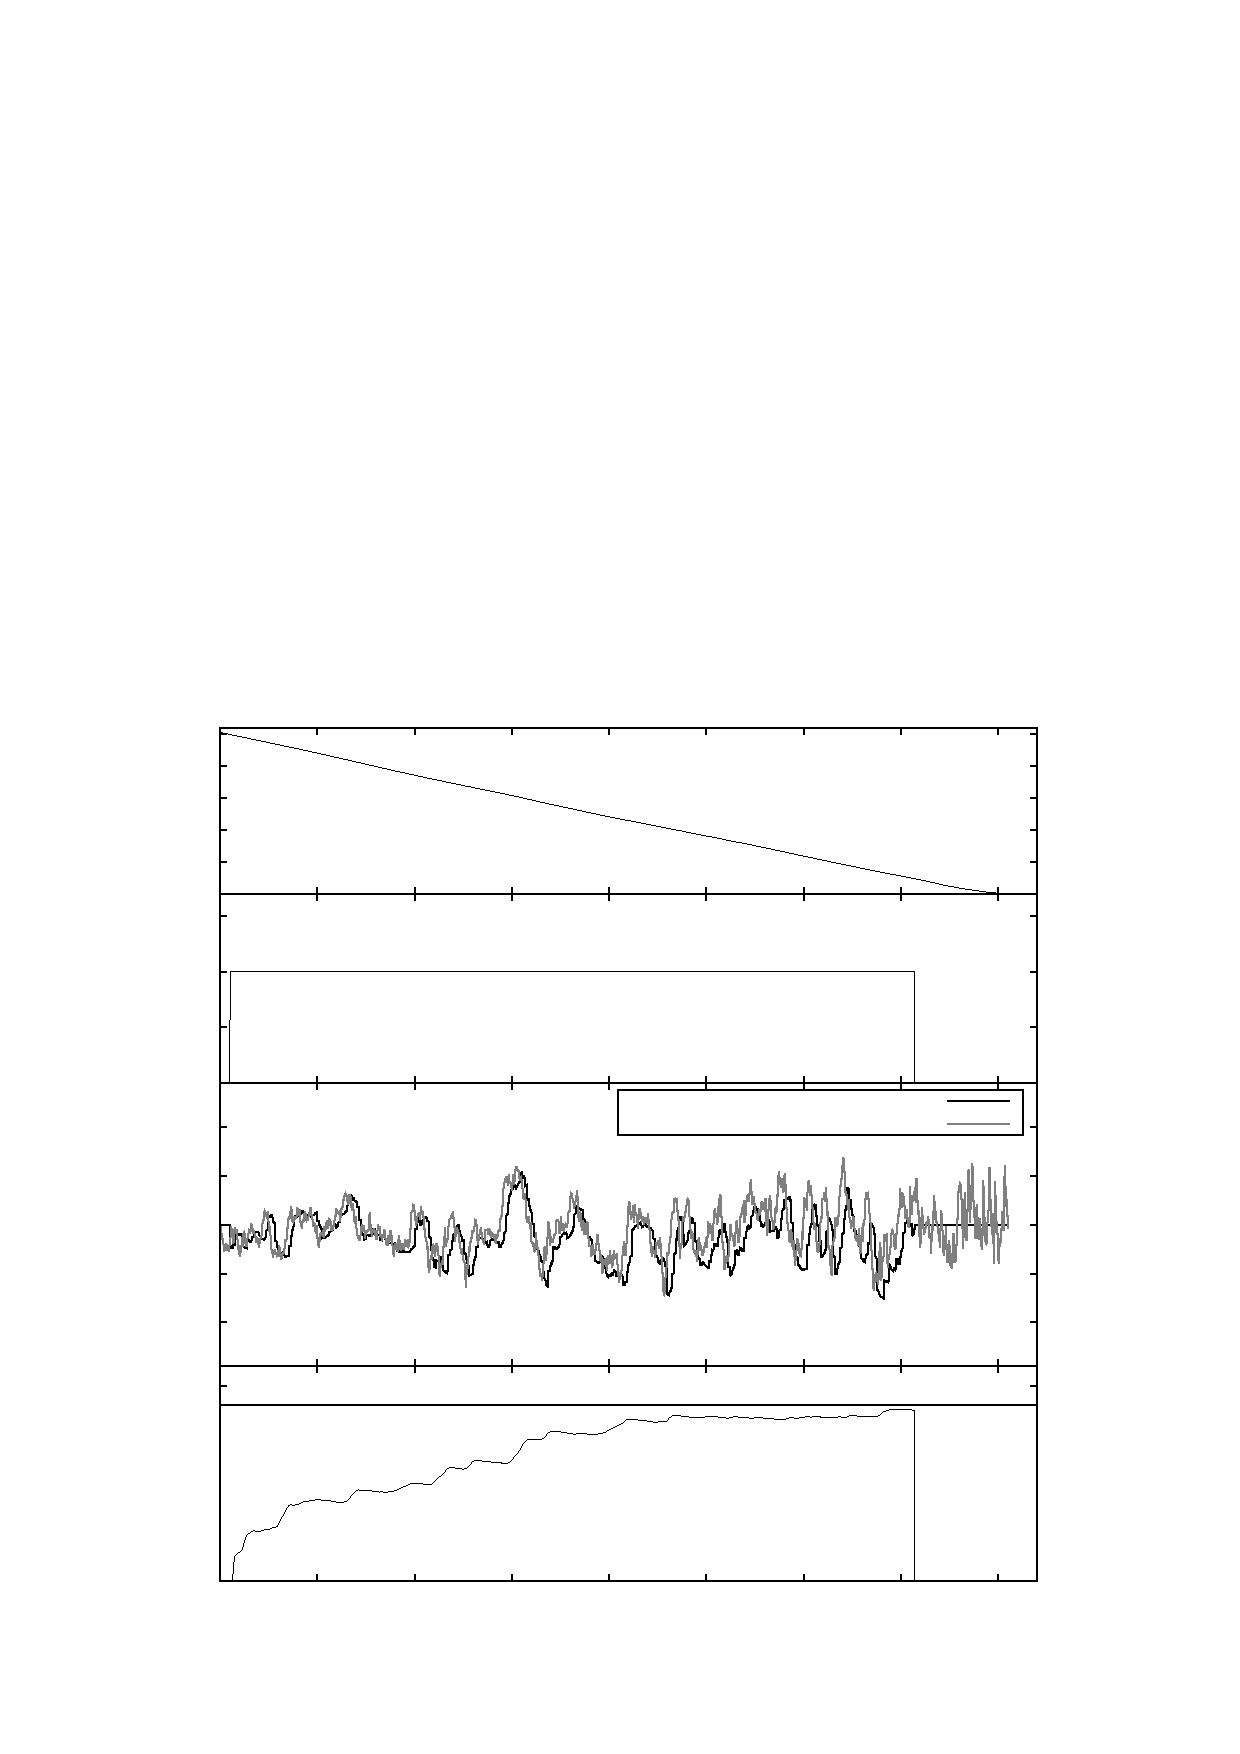
\includegraphics{vertical_wind_estimation_1}}%
    \gplfronttext
  \end{picture}%
\endgroup

		\caption{Vertical Wind Estimation Performance}
	\end{figure}
%
At 500 ft height, the observation is triggered and the vertical wind velocity observation starts. It serves as input for the intensity calculation, illustrated right below. The estimated vertical wind velocity follows the true wind velocity accurately with an almost constant offset due to the integration that is conducted in the estimation algorithm (see equation 3.22). It has to be underlined, that the constant offset is negligible, since the time of observation is huge contrary to the offset and the estimated turbulence intensity does not change significantly after 20 seconds of observation.\\
At the flare begin i.e. at the FIP, the observation is stopped and the last value of the integration is extracted. In the observed case, it can be seen that the true and the estimated turbulence intesity match exactly which is arising from the almost negligible lack between estimated and true vertical wind velocity.
\section{Global performance}
Contrary to the scenario of Fig. 4.1, where the individual performances of the two estimators have been measured and the turbulences were deactivated, this section discusses the overall performance of the algorithm i.e the adequate interaction of the two components under presence of turbulence. In the scenario used in Fig. 4.1 the results of both regarded algorithms were computed uncoupled from the simulation. In this section the complete hard landing predictor is integrated into the simulation, so that the outputs are computed on the flow. This is necessary, since the turbulence estimatior requires measurements ($\alpha(t),n_{z}(t)$) which are easily available on the flow. Comparable to the mentioned scenario, 5000 landings are regarded in which the four parameters and the turbulence are varied within their operational fields. Through recording of the defined three booleans and the true impact velocity it is possible to trace both the contribution of each component to the performance and its contribution to the malfunction. To distinguish, the FoM for both the Statistical Subtrigger's and the Deterministical Subtrigger's FAR are presented seperately.\\
\indent Due to the presence of turbulences, uncertainty is introduced to the calculations. A significant degradation is therefore expected in the global performance. The probability threshold, i.e the tuning parameter is set to a reasonable initial value of five percent. That is why the ratio between FA and MA is expected to change. It is moreover to expect, that a huge part of FA and MA will occur under severe turbulences.\\
Regarding Fig. 4.11, one realisesd that most of the expectations are fulfilled. The balance between FA and MA changed to $[\frac{10}{1}]$, since the tuning parameter has been selected more or less arbitrarily. The mean turbulence level that occured during failed predictions is ($\sigma$=2.8) demonstrating the challenge to predict a hard landing under strong turbulences.    
%	
	\begin{figure}[H]
		% GNUPLOT: LaTeX picture with Postscript
\begingroup
  \makeatletter
  \providecommand\color[2][]{%
    \GenericError{(gnuplot) \space\space\space\@spaces}{%
      Package color not loaded in conjunction with
      terminal option `colourtext'%
    }{See the gnuplot documentation for explanation.%
    }{Either use 'blacktext' in gnuplot or load the package
      color.sty in LaTeX.}%
    \renewcommand\color[2][]{}%
  }%
  \providecommand\includegraphics[2][]{%
    \GenericError{(gnuplot) \space\space\space\@spaces}{%
      Package graphicx or graphics not loaded%
    }{See the gnuplot documentation for explanation.%
    }{The gnuplot epslatex terminal needs graphicx.sty or graphics.sty.}%
    \renewcommand\includegraphics[2][]{}%
  }%
  \providecommand\rotatebox[2]{#2}%
  \@ifundefined{ifGPcolor}{%
    \newif\ifGPcolor
    \GPcolortrue
  }{}%
  \@ifundefined{ifGPblacktext}{%
    \newif\ifGPblacktext
    \GPblacktexttrue
  }{}%
  % define a \g@addto@macro without @ in the name:
  \let\gplgaddtomacro\g@addto@macro
  % define empty templates for all commands taking text:
  \gdef\gplbacktext{}%
  \gdef\gplfronttext{}%
  \makeatother
  \ifGPblacktext
    % no textcolor at all
    \def\colorrgb#1{}%
    \def\colorgray#1{}%
  \else
    % gray or color?
    \ifGPcolor
      \def\colorrgb#1{\color[rgb]{#1}}%
      \def\colorgray#1{\color[gray]{#1}}%
      \expandafter\def\csname LTw\endcsname{\color{white}}%
      \expandafter\def\csname LTb\endcsname{\color{black}}%
      \expandafter\def\csname LTa\endcsname{\color{black}}%
      \expandafter\def\csname LT0\endcsname{\color[rgb]{1,0,0}}%
      \expandafter\def\csname LT1\endcsname{\color[rgb]{0,1,0}}%
      \expandafter\def\csname LT2\endcsname{\color[rgb]{0,0,1}}%
      \expandafter\def\csname LT3\endcsname{\color[rgb]{1,0,1}}%
      \expandafter\def\csname LT4\endcsname{\color[rgb]{0,1,1}}%
      \expandafter\def\csname LT5\endcsname{\color[rgb]{1,1,0}}%
      \expandafter\def\csname LT6\endcsname{\color[rgb]{0,0,0}}%
      \expandafter\def\csname LT7\endcsname{\color[rgb]{1,0.3,0}}%
      \expandafter\def\csname LT8\endcsname{\color[rgb]{0.5,0.5,0.5}}%
    \else
      % gray
      \def\colorrgb#1{\color{black}}%
      \def\colorgray#1{\color[gray]{#1}}%
      \expandafter\def\csname LTw\endcsname{\color{white}}%
      \expandafter\def\csname LTb\endcsname{\color{black}}%
      \expandafter\def\csname LTa\endcsname{\color{black}}%
      \expandafter\def\csname LT0\endcsname{\color{black}}%
      \expandafter\def\csname LT1\endcsname{\color{black}}%
      \expandafter\def\csname LT2\endcsname{\color{black}}%
      \expandafter\def\csname LT3\endcsname{\color{black}}%
      \expandafter\def\csname LT4\endcsname{\color{black}}%
      \expandafter\def\csname LT5\endcsname{\color{black}}%
      \expandafter\def\csname LT6\endcsname{\color{black}}%
      \expandafter\def\csname LT7\endcsname{\color{black}}%
      \expandafter\def\csname LT8\endcsname{\color{black}}%
    \fi
  \fi
  \setlength{\unitlength}{0.0500bp}%
  \begin{picture}(9070.00,4534.00)%
    \gplgaddtomacro\gplbacktext{%
      \csname LTb\endcsname%
      \put(1078,704){\makebox(0,0)[r]{\strut{}-20}}%
      \put(1078,1150){\makebox(0,0)[r]{\strut{}-17.5}}%
      \put(1078,1595){\makebox(0,0)[r]{\strut{}-15}}%
      \put(1078,2041){\makebox(0,0)[r]{\strut{}-12.5}}%
      \put(1078,2487){\makebox(0,0)[r]{\strut{}-10}}%
      \put(1078,2932){\makebox(0,0)[r]{\strut{}-7.5}}%
      \put(1078,3378){\makebox(0,0)[r]{\strut{}-5}}%
      \put(1078,3823){\makebox(0,0)[r]{\strut{}-2.5}}%
      \put(1078,4269){\makebox(0,0)[r]{\strut{} 0}}%
      \put(1210,484){\makebox(0,0){\strut{}-20}}%
      \put(2143,484){\makebox(0,0){\strut{}-17.5}}%
      \put(3076,484){\makebox(0,0){\strut{}-15}}%
      \put(4009,484){\makebox(0,0){\strut{}-12.5}}%
      \put(4941,484){\makebox(0,0){\strut{}-10}}%
      \put(5874,484){\makebox(0,0){\strut{}-7.5}}%
      \put(6807,484){\makebox(0,0){\strut{}-5}}%
      \put(7740,484){\makebox(0,0){\strut{}-2.5}}%
      \put(8673,484){\makebox(0,0){\strut{} 0}}%
      \csname LTb\endcsname%
      \put(176,2486){\rotatebox{-270}{\makebox(0,0){\strut{}$\,$$\widehat{v}_{z,IMP,0,analytical}$$[\frac{ft}{sec}]$}}}%
      \put(4941,154){\makebox(0,0){\strut{}$\,$$v_{z,IMP,0}$ $[\frac{ft}{sec}]$}}%
      \put(5389,2201){\makebox(0,0)[l]{\strut{}$FAR_{total}$}}%
      \put(7292,2201){\makebox(0,0)[l]{\strut{}$=9.20\%$}}%
      \put(5389,1916){\makebox(0,0)[l]{\strut{}$FAR_{DST\, \& \,SST}$}}%
      \put(7292,1916){\makebox(0,0)[l]{\strut{}$=2.96\%$}}%
      \put(5389,1631){\makebox(0,0)[l]{\strut{}$FAR_{DST}$}}%
      \put(7292,1631){\makebox(0,0)[l]{\strut{}$=0.00\%$}}%
      \put(5389,1346){\makebox(0,0)[l]{\strut{}$FAR_{SST}$}}%
      \put(7292,1346){\makebox(0,0)[l]{\strut{}$=6.24\%$}}%
      \put(2068,3289){\makebox(0,0)[l]{\strut{}$MAR_{total}$=1.3\%}}%
      \put(2068,2183){\makebox(0,0)[l]{\strut{}$DR_{total}=96\%$}}%
    }%
    \gplgaddtomacro\gplfronttext{%
    }%
    \gplbacktext
    \put(0,0){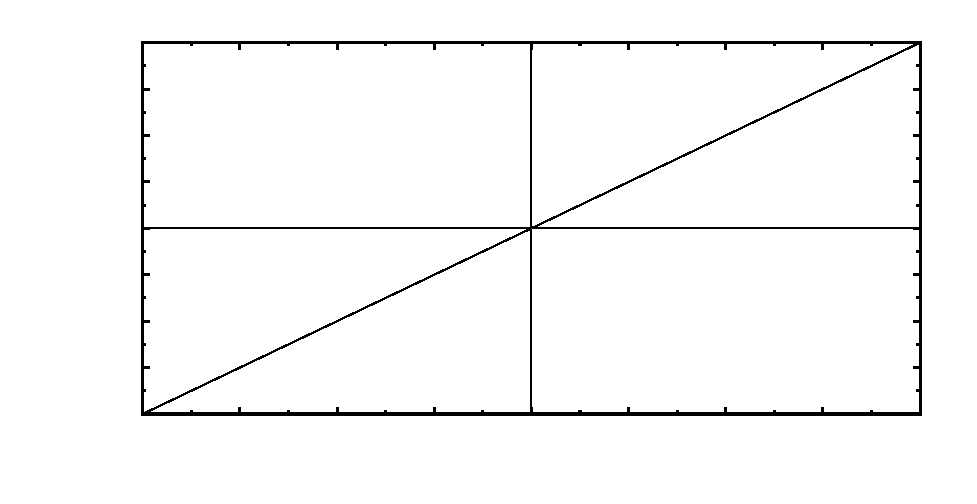
\includegraphics{global_performance}}%
    \gplfronttext
  \end{picture}%
\endgroup

		\caption{Global Algorithm Performance}
	\end{figure}
%
\chapter{Summary}
Driven by globalisation, the air traffic density rises, especially at important airports. Analysing statistics of accidents during the landing phase, one recognises that the mean percentage is caused by flight crew errors and flight operational errors. Automatic landings require an \gls{ILS} device but reduce the pilot's workload during this important flight phase and hence reduce the risk of an incident due to flight crew errors. To reduce the risk of flight operational incidents, it is to discharge frequented airports. That is why the semi automatic landing consisting of a manual approach to the flare initial point and an automatic flare has been proposed. It attempts a reduction of the pilot's workload at an airport without \gls{ILS} device. It further renders the landing easier and is nonetheless a financial benefit to airline companies, since it reduces the afforded pilot training. During this landing the autopilot takes over the \gls{A/C}'s guidance at FIP. It has thus to cope with more demanding initial flare conditions than under fully automatic landings, since a human pilot guided the aircraft during approach. Taking into account that the \gls{A/C} attitude at FIP influences the vertical touchdown velocity, so that a hard landing can occur, the target of this thesis was to propose an algorithm that predicts at FIP if the landing will be hard - or not. At the moment this thesis has been written a literature review lead to the result, that there is no comparable invention up to now.\\
\indent An analysis of the automatic flare has been conducted during a first step of this thesis, to detect parameters with an impact on the touchdown velocity. It has been seperated between parameters with a deterministic influence and parameters with a random influence.\\
Based on the classification of the parameters a complementary algorithm design has been proposed to cope with the uncertainty that turbulences evoke on the predictability of the touchdown velocity. It is thus possible to reduce the uncertainty and therefore to augment the prediction performance.\\ 
The primary complement of the proposed algorithm targets the calculation of the touchdown velocity caused by the deterministic parameters. Two methods of the deterministic calculation have been theoretically discussed, implemented and assessed. The first one is a conventional, analytical formula, considering the flight mechanics of an automatic flare. The second one is an automatically build FIS. A comparision between both methods elucidated a huge discrepancy in the performances. The inferior result of the analytical formula is caused by several simplifications that have been considered to describe the highly non-linear process of an automatic flare. Given the fact, that an improvement of the analytical formula's performance is time consuming while the \gls{ANFIS} algorithms fullfills all requirements in terms of computational effort as well as prediction performance and tracebility, it has no longer been considered as an alternative. This algorithm which is to the present almost undetected in aviation environment is worth to be considerrd in future algorithm design.\\
The second complement of the proposed predictor estimates the vertical wind to determine the stochastically influencing parameter i.e. the turbulence intensity during the landing. A new method of onboard vertical wind estimation, leading to accurate results has therefore been designed.\\
Both complementary outputs are merged in the last module of the suggested predictor, where the probability of a hard landing is computed based on the outputs of the two complements and a statistical formula.\\
A detailed analysis of the developed algorithm demonstrates the performance of each algortithm's part. Moreover it depicts the performance augmentation that is reached under use of the complementary design. It nevertheless remains a challenge to predict a randomly influenced value.\\
\indent A viable augmentation of the prediction performance can be reached by adjusting the algorithm's tuning parameter. Nonetheless the prediction performance could be augmented through inserting a hardware device in the \gls{A/C} in order to more precisely estimate the turbulences in front of the \gls{A/C}.
%
\newpage
%
\bibliographystyle{chicago}
\bibliography{Thesis}
% nocite puts a bib-reference that has NOT been within the text into the outline of the bibliography
\nocitet{Slawinski1999}
\nocite{Anthony1989}
\nocite{Seckel1975}
\nocite{Stewart2003}

\end{document}
%%%%%%%%%%%%%%%%%%%%%%%%%%%%%%%%%%%%%%%%%%%%%%%%%%%%%%%%%%%%%%%%%%%%%%%%%%%%%%%%%%%%%%%%%%%%%%%%%%%%%%%%%%%%%%%%%%%%%%%%%%%%%%
%%%%%%%%%%%%%%%%%%%%%%%%%%%%%%%%%%%%%%%%%%%%%%%%%%%%%%%%%%%%%%%%%%%%%%%%%%%%%%%%%%%%%%%%%%%%%%%%%%%%%%%%%%%%%%%%%%%%%%%%%%%%%%
%%%%%%%%%%%%%%%%%%%%%%%%%%%%%%%%%%%%%%%%%%%%%%%%%%%%%%%%%%%%%%%%%%%%%%%%%%%%%%%%%%%%%%%%%%%%%%%%%%%%%%%%%%%%%%%%%%%%%%%%%%%%%